% Options for packages loaded elsewhere
\PassOptionsToPackage{unicode}{hyperref}
\PassOptionsToPackage{hyphens}{url}
%
\documentclass[
  12pt,
]{article}
\usepackage{lmodern}
\usepackage{amsmath}
\usepackage{ifxetex,ifluatex}
\ifnum 0\ifxetex 1\fi\ifluatex 1\fi=0 % if pdftex
  \usepackage[T1]{fontenc}
  \usepackage[utf8]{inputenc}
  \usepackage{textcomp} % provide euro and other symbols
  \usepackage{amssymb}
\else % if luatex or xetex
  \usepackage{unicode-math}
  \defaultfontfeatures{Scale=MatchLowercase}
  \defaultfontfeatures[\rmfamily]{Ligatures=TeX,Scale=1}
\fi
% Use upquote if available, for straight quotes in verbatim environments
\IfFileExists{upquote.sty}{\usepackage{upquote}}{}
\IfFileExists{microtype.sty}{% use microtype if available
  \usepackage[]{microtype}
  \UseMicrotypeSet[protrusion]{basicmath} % disable protrusion for tt fonts
}{}
% \makeatletter
% \@ifundefined{KOMAClassName}{% if non-KOMA class
%   \IfFileExists{parskip.sty}{%
%     \usepackage{parskip}
%   }{% else
%     \setlength{\parindent}{0pt}
%     \setlength{\parskip}{6pt plus 2pt minus 1pt}}
% }{% if KOMA class
%   \KOMAoptions{parskip=half}}
% \makeatother
\usepackage{xcolor}
\IfFileExists{xurl.sty}{\usepackage{xurl}}{} % add URL line breaks if available
\IfFileExists{bookmark.sty}{\usepackage{bookmark}}{\usepackage{hyperref}}
\hypersetup{
  hidelinks,
  pdfcreator={LaTeX via pandoc}}
\urlstyle{same} % disable monospaced font for URLs
\usepackage[margin=1in]{geometry}
\usepackage{longtable,booktabs}
\usepackage{calc} % for calculating minipage widths
% Correct order of tables after \paragraph or \subparagraph
\usepackage{etoolbox}
\makeatletter
\patchcmd\longtable{\par}{\if@noskipsec\mbox{}\fi\par}{}{}
\makeatother
% Allow footnotes in longtable head/foot
\IfFileExists{footnotehyper.sty}{\usepackage{footnotehyper}}{\usepackage{footnote}}
\makesavenoteenv{longtable}
\usepackage{graphicx}
\makeatletter
\def\maxwidth{\ifdim\Gin@nat@width>\linewidth\linewidth\else\Gin@nat@width\fi}
\def\maxheight{\ifdim\Gin@nat@height>\textheight\textheight\else\Gin@nat@height\fi}
\makeatother
% Scale images if necessary, so that they will not overflow the page
% margins by default, and it is still possible to overwrite the defaults
% using explicit options in \includegraphics[width, height, ...]{}
\setkeys{Gin}{width=\maxwidth,height=\maxheight,keepaspectratio}
% Set default figure placement to htbp
\makeatletter
\def\fps@figure{htbp}
\makeatother
\setlength{\emergencystretch}{3em} % prevent overfull lines
\providecommand{\tightlist}{%
  \setlength{\itemsep}{0pt}\setlength{\parskip}{0pt}}
\setcounter{secnumdepth}{-\maxdimen} % remove section numbering
\usepackage{booktabs}
\usepackage{longtable}
\usepackage{array}
\usepackage{multirow}
\usepackage{wrapfig}
\usepackage{float}
\usepackage{colortbl}
\usepackage{xcolor}
\usepackage{pdflscape}
\usepackage{tabu}
\usepackage{threeparttable}
\usepackage{threeparttablex}
\usepackage[normalem]{ulem}
\usepackage{makecell}
\definecolor{Blue}{rgb}{0.01,0.28,1.0}
\definecolor{Maroon}{rgb}{0.5,0.0,0.0}
\definecolor{darkgreen}{RGB}{0,150,0}
\hypersetup{colorlinks=true, citecolor=Blue, urlcolor=Maroon}
%%\renewcommand{\thetable}{S\arabic{table}} 
%%\renewcommand{\thefigure}{S\arabic{figure}} 
%%\renewcommand{\theequation}{S\arabic{equation}}
\usepackage[modulo]{lineno}
%% for longtable
\setlength{\LTcapwidth}{\textwidth} %% long table caption width=\textwidth
\usepackage[font=small]{caption} %% caption text size=\normalsize
%% header
\usepackage{fancyhdr}
\pagestyle{fancy}
\setlength\headheight{36pt}
\renewcommand\headrulewidth{0pt}
\fancyhead[L]{
\includegraphics[width=6.5cm]{figs_article/NatureComm_logo.png}}
\fancyhead[C]{}
\fancyhead[R]{Submitted Manuscript: Confidential}
\usepackage[numbers, round, comma]{natbib}
\usepackage{etoolbox} %% Several bib, see: https://tex.stackexchange.com/questions/69675/how-to-set-the-number-of-the-first-citation
%%\def\bibfont{\footnotesize}
\usepackage{booktabs}
\usepackage{longtable}
\usepackage{array}
\usepackage{multirow}
\usepackage{wrapfig}
\usepackage{float}
\usepackage{colortbl}
\usepackage{pdflscape}
\usepackage{tabu}
\usepackage{threeparttable}
\usepackage{threeparttablex}
\usepackage[normalem]{ulem}
\usepackage{makecell}
\usepackage{xcolor}
\ifluatex
  \usepackage{selnolig}  % disable illegal ligatures
\fi
%\usepackage[]{natbib}
%\bibliographystyle{bib/naturemag.bst}

\author{}
\date{}

\begin{document}

\renewcommand{\bibsection}{}  %% No section name for bibliography
~
\vspace{-0.25cm}
\begin{center}
  \LARGE{Forest refuge areas and carbon emissions from tropical deforestation in the 21\textsuperscript{st} century}
\end{center}

\vspace{0.5cm}

\begin{center}
  \large{
  Ghislain VIEILLEDENT$^{[\star, 1, 2, 3, 4]}$ \hspace{0.5cm} Christelle VANCUTSEM$^{[1]}$\\
  \vspace{0.5cm}
  and \hspace{0.5cm} Frédéric ACHARD$^{[1]}$
  }
\end{center}

\vspace{0.5cm}

\begin{center}
  $[\star]$ \textbf{Correspondence to:}~ghislain.vieilledent@cirad.fr\\
\end{center}

\vspace{0.5cm}

{\small
  \begin{flushleft}
    $[1]$ \textbf{European Commission}, JRC, Bio-economy Unit, I-21027 Ispra (VA), ITALY\\
    $[2]$ \textbf{CIRAD}, UPR Forêts et Sociétés, F-34398 Montpellier, FRANCE\\
    $[3]$ \textbf{CIRAD}, UMR AMAP, F-34398 Montpellier, FRANCE\\
    $[4]$ AMAP, \textbf{Univ Montpellier}, CIRAD, CNRS, INRAE, IRD, Montpellier, FRANCE\\
  \end{flushleft}}

%\newpage

\linenumbers

\hypertarget{abstract}{%
\section*{Abstract}\label{abstract}}
\addcontentsline{toc}{section}{Abstract}

\textbf{Tropical forests are disappearing at an alarming rate due to human activities. Here, we provide spatial models of deforestation in 92 countries covering all the tropical moist forests in the world. Our models confirm the effectiveness of protected areas in displacing deforestation and the negative impact of roads and landscape fragmentation on forest conservation in the tropics. Using our models, we derive high-resolution pantropical maps of the deforestation risk and future forest cover for the 21\textsuperscript{st} century under a ``business-as-usual'' scenario based on the deforestation rates observed in the 2010s. Although under this scenario, large areas of tropical moist forest should remain in the heart of the Amazon, in the Congo Basin, and in New Guinea in 2100, 54\% (46--61\%) of all forest cover is expected to disappear during the course of the 21\textsuperscript{st} century, and many countries will have lost all their forests by 2100. The remaining forests will be highly fragmented and located in remote places. As future deforestation will concern forests with higher aboveground carbon stocks, annual carbon emissions associated with tropical deforestation are expected to increase by +0.221~Pg/yr (+42\%) between the 2010s and the 2070s.}\\

% \textbf{Keywords:} deforestation, forecasts, forest cover change, forest refuge areas, moist tropical forests, spatial modelling, scenarios.
% 
% \textbf{One sentence summary:} Anthropogenic deforestation will affect tropical forests with higher carbon stocks in the future.

\newpage

%% =========================================================================================
%% MAIN TEXT
%% =========================================================================================

\indent Tropical forests are at the heart of concerns when it comes to climate change and biodiversity loss, which both pose unprecedented threats to human civilization \citep{IPCC2014, Cardinale2012}. Commonly called the ``Jewels of the Earth'', tropical forests shelter 30 million species of plants and animals, representing half of the Earth's wildlife and at least two-thirds of its plant species \citep{Gibson2011, Wilson2012}. Through carbon sequestration, they play an important role in the global carbon cycle and regulate the global climate \citep{Baccini2017}. Intact tropical forest ecosystems also prevent outbreaks of zoonoses and reduce the risk of pandemics \citep{Tollefson2020}. At local scale, tropical forests regulate the regional climate \citep{Dickinson1992}, cooling the atmosphere \citep{Ellison2017}, and facilitate access to water \citep{Ellison2017, Zhang2021}. They also protect against erosion and flooding \citep{Bradshaw2007}. Close to 1.6 billion people (a quarter of the world's population) rely on forest resources for their livelihoods \citep{FAO2015}. Despite the many ecosystem services they provide, tropical forests are disappearing at an alarming rate \citep{FAO2015, Hansen2013, Vancutsem2021, Achard2014}, mostly because of human activities \citep{Curtis2018, Geist2002}. Past studies have estimated that about 8~Mha of tropical forest (including moist and dry forests) are currently disappearing each year \citep{FAO2015}. At this rate, will there still be any tropical forests left at the end of the 21\textsuperscript{st} century, if so, where will they be concentrated, and what will be the consequences of tropical deforestation on climate and biodiversity in the future?\\

Forecasting forest cover change is paramount as it allows us to foresee the consequences of deforestation (in terms of carbon emissions, biodiversity loss, or water supply) under various technological, political, and socio-economic scenarios, and to inform decision makers accordingly \citep{Clark2001}. The ``business-as-usual'' scenario is of particular interest as it makes it possible to predict the likely future in the absence of change in deforestation rates, and if necessary, to alert decision-makers to an essential change of course to avoid any potential environmental disaster. While models and scenarios of carbon dioxide emission and climate change have been developed for several years by the Intergovernmental Panel on Climate Change \citep{IPCC2014} and are now widely used by the scientific community and known to the general public, equivalent models and scenarios for land-use change and biodiversity at the global scale are still relatively scarce \citep{Pereira2020}. Moreover, baseline scenarios of deforestation and associated carbon dioxide emission are necessary for implementing REDD+ (Reducing Emissions from Deforestation and forest Degradation) activities in the framework of the Paris Agreement on climate change \citep{Goetz2015}. Spatialized forest cover change scenarios are crucial because both forest carbon stocks \citep{Baccini2017, Avitabile2016} and biodiversity \citep{Kremen2008, Mittermeier2011} vary considerably in space at fine scale. Non-spatial scenarios of forest cover change \citep{FAO2015} cannot be used to forecast associated carbon emissions and change in biodiversity accurately, or for systematic conservation planning at the local scale. Spatial forecasts of forest cover change are based on spatial statistical models, which enable estimation of a probability of change in space as a function of a set of spatial predictors \citep{Rosa2014}. In addition to forecasts, statistical models can be used to identify the main drivers of deforestation and to quantify their relative effects. For example, models can be used to assess the impact of roads on the risk of deforestation \citep{Laurance2014} and the effectiveness of protected areas at reducing deforestation \citep{Andam2008, Wolf2021}.\\

Few authors have attempted to provide spatialized forest cover change scenarios in the tropics at large spatial scales. The largest studies to date have focused on modelling and forecasting forest cover change at the scale of the Amazonian basin \citep{Aguiar2016, Swann2015, Soares-Filho2006}. In this paper, we model and forecast tropical deforestation at the pantropical scale using high-resolution spatial data. This was made possible by the recent availability of pantropical spatial datasets of forest cover change \citep{Vancutsem2021} and of global spatial datasets of explanatory factors related to deforestation at the required resolution (World Database on Protected Areas, SRTM Digital Elevation Database, and OpenStreetMap). We combine these extensive datasets in a spatial statistical model to test the effectiveness of protected areas at reducing deforestation and to assess the impact of roads on the risk of deforestation. Assuming a business-as-usual scenario, we derive high-resolution maps of deforestation risk and future forest cover over the 21\textsuperscript{st} century in the humid tropics. We also estimate the carbon emissions associated with projected deforestation and conduct an uncertainty analysis.

\hypertarget{remaining-tropical-moist-forests-in-2100}{%
\section{Remaining tropical moist forests in 2100}\label{remaining-tropical-moist-forests-in-2100}}

Using Vancutsem \emph{et al.}'s study \citep{Vancutsem2021} as a reference, we estimate that around 7.6~Mha (5.8--9.5~Mha) of tropical moist forest have been disappearing each year over the last decade (2010--2020). This corresponds to an area of 76,000~km\textsuperscript{2}, about the size of Scotland or South Carolina, which is deforested each year. We show here that under a business-as-usual scenario of deforestation, 54\% (46--61\%) of the world's tropical moist forest will disappear over the course of the 21\textsuperscript{st} century (Fig.~\ref{fig:fcc2100} and Table~\ref{tab:fcc}) but with marked differences in the percentage of forest cover loss at the continental (Fig.~\ref{fig:perc-loss} and Table~\ref{tab:fcc}) and country (tables~S14--S17) scales. In Southeast Asia, where the forest area remaining in 2020 was relatively low (247~Mha) and the area deforested each year is relatively large (2.5~Mha/yr) compared to the two other continents, the percentage of forest cover loss over the 21\textsuperscript{st} century will reach 78\%. In Africa, where the annual deforested area is lower (2.2~Mha/yr), this percentage will be 58\%. In Latin America, where the annual deforested area is higher (2.9~Mha/yr), but where the remaining tropical moist forest in 2020 is also much larger than in Southeast Asia and Africa (621~Mha), this percentage will be 41\%. Under a business-as-usual scenario of deforestation, three quarters of the tropical moist forests that existed in 2000 will have disappeared around years 2100, 2150, and 2200 in Southeast Asia, Africa, and Latin America, respectively (Fig.~\ref{fig:perc-loss} and Table~\ref{tab:fcc}).\\

At the country scale, we predict that 47 countries (18 in Latin America, 21 in Africa, and 8 in Southeast Asia) out of the 92 we studied, plus 18 states in Brazil and one region in India, will lose all their tropical forests by 2100 (Fig.~\ref{fig:fcc2100} and table~S16). Among these countries or regions, 20 countries (six in America, eight in Africa, and six in Asia), five states in Brazil, and one region in India had more than one million hectares of forest in 2020. These 20 countries include most of the countries of Central America (Mexico, Guatemala, Honduras, Nicaragua), Western (Sierra Leone, Ivory Coast, Ghana, Nigeria) and Eastern (Ethiopia, Madagascar) Africa, and continental Southeast Asia (Myanmar, Laos, Vietnam, Cambodia, Malaysia, Indian Western Ghats). These regions include almost all tropical forests located within six biodiversity hotspots identified by Mittermeier \emph{et al.} \citep{Mittermeier2011}: Mesoamerica, Guinean Forests of West Africa, the Horn of Africa, Madagascar and Indian Ocean Islands, Indo-Burma, Western Ghats and Sri Lanka (Fig.~\ref{fig:fcc2100}).\\

\newpage

Using a spatial statistical modelling approach (see Methods, figs.~S1--S9, and tables~S1--S3), we obtain high resolution (30~m) pantropical maps of the deforestation risk (Fig.~\ref{fig:prob} and fig.~S10) and project forest cover for the 21\textsuperscript{st} century in the humid tropics (Fig.~\ref{fig:fcc2100} and fig.~S11) under a business-as-usual scenario. Three large ``blocks'' of relatively intact tropical moist forest will remain in 2100 (see both Fig.~\ref{fig:fcc2100} and the interactive map of projected deforestation for the period 2020--2100 available at \url{https://forestatrisk.cirad.fr/maps.html}). One forest block will be located in Latin America and will include the upper part of the Amazonian basin (including the Peruvian, Ecuadorian, Colombian and Venezuelan Amazonia) and the Guiana Shield (Guyana, Suriname, and French Guiana). The second block will be located in the western part of the Congo basin and will include forests in Gabon, Equatorial Guinea, Cameroon, the Central African Republic, and the Republic of Congo. The third block will be located in Melanesia and will include forests in Papua New Guinea, Solomon Islands, and Vanuatu.\\

Apart from these three large and relatively intact forest blocks, the tropical moist forest remaining in 2100 will be highly fragmented (Fig.~\ref{fig:fcc2100}). In Latin America, highly fragmented forests will be found in the Brazilian states of the Amazonian deforestation arc (Acre, Rondonia, Mato Grosso, Para, Amapa) and in the Roraima state in the northern Amazonia. In Africa, forests in the Democratic Republic of the Congo (DRC) will also be highly fragmented (fig.~S11) and will be completely separated from the large forest block located in the western part of the Congo basin (Fig.~\ref{fig:fcc2100}). In Southeast Asia, small patches of heavily fragmented forests will remain in Thailand, Indonesia, and the Philippines (Fig.~\ref{fig:fcc2100}). The remaining forests will be concentrated in remote areas (far from roads and towns), preferentially in protected areas, and at high elevations (Figs.~\ref{fig:fcc2100},~\ref{fig:prob} and tables~S6--S9). For example, the remaining forests of Borneo will be concentrated in the Betung Kerihun and Kayan Mentarang National Parks.\\

As tropical forests shelter a large proportion of terrestrial biodiversity and carbon stocks on land, future tropical deforestation is expected to have strong negative impacts on both biodiversity and climate. The impact of projected deforestation on carbon emissions is discussed below, but rigorous assessment of the impact of projected deforestation on biodiversity is beyond the scope of this study. Such an impact analysis would require accurate species distribution and biodiversity maps including a large number of species representative of the biodiversity in the tropics. Such maps are not available to date \citep{Pimm2014}. Nonetheless, as a rough estimate, if we consider only endemic species \citep{Mittermeier2011} in the six biodiversity hotspots where almost all the tropical forest is predicted to disappear by 2100, and assume that most of these species depend on tropical moist forests, deforestation would lead to the extinction of 29,140 species of plants and 4,576 species of vertebrates (including birds, reptiles, amphibians, freshwater fishes, and mammals) which cannot be found anywhere else on Earth (table~S18).

\newpage

\hypertarget{carbon-emissions-under-a-business-as-usual-scenario-of-deforestation}{%
\section{Carbon emissions under a business-as-usual scenario of deforestation}\label{carbon-emissions-under-a-business-as-usual-scenario-of-deforestation}}

Here we estimate the aboveground carbon emissions associated with deforestation projected for the period 2020--2100 under a business-as-usual scenario of deforestation. When computing carbon emissions associated with projected deforestation, we assume that the carbon stocks of existing forests will remain stable in the future. Under a business-as-usual scenario of deforestation (i.e., constant annual deforested area), the change in predicted annual carbon emissions is only attributable to the location of the future deforestation (Fig.~\ref{fig:fcc2100} and fig.~S11) and to the spatial distribution of forest carbon stocks (fig.~S12). We find that annual carbon emissions associated with deforestation of tropical moist forests will increase from 0.525~Pg/yr in 2010--2020 to 0.746~Pg/yr in 2070--2080, which corresponds to a 42\% increase (Fig.~\ref{fig:c-em}). This increase in annual carbon emissions is predicted for all three continents (Fig.~\ref{fig:c-em}). A decrease in carbon emissions is then predicted starting from the period 2070--2080 for Southeast Asia and the period 2080--2090 at pantropical scale (Fig.~\ref{fig:c-em}).\\

The predicted increase in annual carbon emissions is explained by the fact that the forests which will be deforested in the future have higher carbon stocks. Several studies have shown that elevation is an important variable in determining forest carbon stocks \citep{Vieilledent2016, Saatchi2011}. Forest carbon stocks are expected to be optimal at mid-elevation \citep{Vieilledent2016} due to higher orographic precipitation at this elevation and because the climatic stress associated with winds and temperature is lower at mid-elevation than at high elevation. Here, we show that low-elevation areas are more deforested than high-elevation areas (tables~S4, S5). This is explained by the fact that low-elevation areas are more accessible to human populations and by the fact that arable lands are concentrated at low elevation, where the terrain slope is usually lower and the soil is more productive \citep{Geist2002}. Consequently, the predicted increase in carbon emissions can be explained by the fact that deforestation will move towards higher elevation areas where forest carbon stocks are higher. Moreover, remote forest areas that have been less disturbed by human activities in the past have accumulated large quantities of carbon \citep{Dargie2017, Brinck2017}. The progressive deforestation of more intact forests also explains the predicted increase in carbon emissions.\\

The decrease in carbon emissions predicted from the period 2070--2080 for Southeast Asia, and from the period 2080--2090 at pantropical scale, can be associated with a decrease in carbon stocks of deforested areas (in association with environmental factors, such as lower carbon stocks at very high elevation) or a decrease in the total deforested area at the continental and global scale, as countries progressively lose all their forest. In Southeast Asia, six countries will lose all their forest between 2070 and 2100 (table~S16). These countries (which include Laos, Malaysia, Myanmar, and Vietnam) account for a significant proportion (32\%) of the annual deforested area in Southeast Asia (808,363~ha/yr out of 2,532,985~ha/yr, see tables~S14, S15). This largely explains the predicted decrease in carbon emissions in Southeast Asia from 2070 on.\\

\newpage

Our estimates of 0.525~Pg/yr (0.208, 0.199, and 0.118~Pg/yr for Latin America, Southeast Asia, and Africa, respectively) of aboveground carbon emissions due to tropical deforestation for the period 2010--2020 are consistent with those of previous studies \citep{Baccini2017, Achard2014, Harris2012}. For the period 2000--2014, previous studies estimated 0.81--0.88~Pg/yr of carbon emissions associated with deforestation considering both moist and dry tropical forests, while our study only focuses on tropical \emph{moist} forests. Because of the projected 42\% increase in carbon emissions associated with tropical deforestation under a business-as-usual scenario, tropical forests will act as an increasing net carbon source \citep{Baccini2017}, thus reinforcing climate change in the future.\\

These results demonstrate the importance of spatial predictions of deforestation to forecast carbon emissions associated with future deforestation. Using mean annual forest cover change estimates per country and forest type (such as those provided by the Forest Resource Assessment report \citep{FAO2015}) and mean forest carbon stocks per continent and forest type (such as the emission factors provided by IPCC \citep{IPCC2019}), it is not possible to predict future trends in carbon emissions associated with deforestation. Under a business-as-usual scenario of deforestation, projected carbon emissions will result from the combination of the spatial variation in forest carbon stocks and the location of the future deforestation.

\hypertarget{effectiveness-of-protected-areas-at-displacing-deforestation}{%
\section{Effectiveness of protected areas at displacing deforestation}\label{effectiveness-of-protected-areas-at-displacing-deforestation}}

Forested protected areas are usually located in areas of high or unique biodiversity, in a non-random way. They are also usually found in remote places with less human disturbances and reduced accessibility, i.e.~far from roads or cities, and usually at higher elevation (fig.~S6), because low-lying arable lands have already been preempted for agriculture \citep{Geist2002}. As a consequence, it is usually difficult to unravel the effect of protected areas from other correlated variables, for example distance to the nearest road, city, or elevation \citep{Andam2008}. The multivariate logistic regression model we use makes it possible to disentangle the effect of each explanatory variable in the spatial deforestation process. Moreover, the spatial random effects included in our model (see Methods and figs.~S8,~S9) correct the potential bias in the protected area effect that could be associated with other unmeasured confounding variables, such as population density \citep{Andam2008}.\\

Here we show that protected areas significantly reduce the risk of deforestation in 74 study areas out of 119 (62\% of the study areas). These 74 study areas accounted for 88\% of the tropical moist forest in 2010 (table~S6). On average, protected areas reduce the risk of deforestation by 40\% (Figs.~\ref{fig:prob},~\ref{fig:proba-var} and table~S5). This result clearly demonstrates the efficiency of protected areas at reducing the spatial risk of deforestation in the tropics. In a recent global study, Wolf \emph{et al.} \citep{Wolf2021} found that protected areas reduced deforestation rates by 41\%, close to the 40\% we find here by focusing on tropical moist forests. Most of the previous studies have assessed the effect of protected areas at reducing deforestation in particular countries or regions \citep{Andam2008, Bruner2001} or at efficiently protecting a particular group of species \citep{Cazalis2020}. Studies at the global scale \citep{Wolf2021, Yang2021} were at 1~km resolution and used spatial matching methods and tree cover loss data \citep{Hansen2013}. Our pantropical approach is based on more accurate forest cover change maps in the humid tropics, in particular in Africa \citep{Vancutsem2021}, and accounts for fine scale deforestation factors acting at a much smaller distance than the distance imposed by a 1~km resolution (see the effect of the distance to forest edge discussed below). Moreover, contrary to most spatial matching methods \citep{Andam2008, Schleicher2019}, the statistical model we use allows us to account for any potential confounding variables which might skew the estimated effect of protected areas.\\

Like other studies reporting the effect of protected areas on deforestation, our study demonstrates that protected areas are effective at \emph{displacing} deforestation outside protected areas in tropical countries, but not necessarily that protected areas play a role in \emph{reducing} the deforestation intensity per se. Indeed, the factors that drive the intensity of deforestation at the country scale are more socio-economic or political, such as the level of economic development, which determines people's livelihood and the link between people and deforestation \citep{Geist2002}, the size of the population \citep{Barnes1990}, or the environmental policy \citep{Soares-Filho2014}. In tropical countries with weak governance (where environmental law enforcement is low) and with a low level of development (where the pressure on forest is high), it is very unlikely that protected areas will remain forested. Under a business-as-usual scenario of deforestation, we assume that the deforestation intensity will remain constant over time. When all the forest outside the protected areas is deforested, deforestation is expected to occur inside protected areas (Fig.~\ref{fig:fcc2100}). In this scenario, protected areas are efficient at protecting forest areas of high and unique biodiversity in the medium term, i.e., forests will be concentrated in protected areas, where the probability of deforestation is lower. In the long term, under a business-as-usual scenario, forests should completely disappear from protected areas while deforestation continues (Fig.~\ref{fig:fcc2100}). This phenomenon is already clearly visible in countries or states where deforestation is advanced, such as in Rondonia state (Brazil) in South America \citep{Ribeiro2005}, Ivory Coast \citep{Sangne2015} or Madagascar \citep{Vieilledent2020} in Africa, or Cambodia \citep{Davis2015} in Southeast Asia. In these countries, several forested protected areas have been entirely deforested (e.g., the Haut-Sassandra protected forest in Ivory Coast, or the PK-32 Ranobe protected area in Madagascar) or severely deforested (e.g., the Beng Per wildlife sanctuary in Cambodia).

\hypertarget{impact-of-roads-and-distance-to-forest-edge-on-the-deforestation-risk}{%
\section{Impact of roads and distance to forest edge on the deforestation risk}\label{impact-of-roads-and-distance-to-forest-edge-on-the-deforestation-risk}}

Here we find that a longer distance to the road significantly reduces the risk of deforestation in 59 study areas out of 119 (50\% of the study areas). These 59 study areas accounted for 90\% of the tropical moist forest in 2010 (table~S7). On average, a distance of 10~km from a road reduces the risk of deforestation by 13\% (Figs.~\ref{fig:prob},~\ref{fig:proba-var} and tables~S5,~S9). This said, opening a road in the forest leads to the creation of two forest edges and computing a distance from a forest pixel to the nearest road implies the existence of a distance to the forest edge. When studying the effect of roads on deforestation, it is thus impossible to neglect the effect of the distance to forest edge on the risk of deforestation.\\

Here, we find that the distance to the forest edge is the most important variable in determining the risk of deforestation (table~S5), in agreement with the results of other studies showing the impact of forest fragmentation on the risk of deforestation in the tropics \citep{Hansen2020}. We estimate that, on average, a distance of 1~km from the forest edge reduces the risk of deforestation by 93\%, and a distance of 10~km reduces the risk of deforestation by almost 100\% (Figs.~\ref{fig:prob},~\ref{fig:proba-var} and tables~S5,~S9).\\

Consequently, building new roads in non-forest areas but close to existing forest edges would significantly increase the risk of deforestation in the nearby forest. This negative impact would be even greater if new roads are opened in the heart of forest areas. In addition to the direct deforestation associated with road building in the forest \citep{Kleinschroth2017}, this would involve creating new forest edges and would dramatically increase deforestation probability in the area concerned. While road networks are expanding rapidly worldwide, notably in remote areas in tropical countries \citep{Laurance2014}, our results underline the importance of conserving large roadless connected (unfragmented) forest areas.

\hypertarget{uncertainty-and-alternative-deforestation-scenarios}{%
\section{Uncertainty and alternative deforestation scenarios}\label{uncertainty-and-alternative-deforestation-scenarios}}

Despite the uncertainty surrounding the mean annual deforested area for each country (figs.~S13,~S14 and table~S20), the consequences of a business-as-usual deforestation scenario on the loss of biodiversity and carbon emissions by 2100 remain clear and alarming (Figs.~\ref{fig:perc-loss},~\ref{fig:c-em} and data~S1,~S2). Moreover, given the current global context, the business-as-usual deforestation scenario we examine here appears to be very conservative. For example, we do not account for the effect of future population growth \citep{Raftery2012}, which will likely have a major effect on deforestation, particularly in Africa, where a large part of the population depends on slash-and-burn agriculture for their livelihood \citep{Barnes1990, Vieilledent2020}. Nor do we account for the increasing demand for agricultural commodities from the tropics, such as palm oil, beef and soybean, which will likely lead to a significant increase in deforestation \citep{Strona2018, Karstensen2013}. Although some conservation strategies, such as protected areas, can help save some time in the fight against deforestation (being efficient at displacing deforestation toward areas of lower biodiversity or carbon stocks), it is extremely urgent to find political and socio-economic solutions that are efficient at curbing deforestation in the long term. Several initiatives involving actors from the political and economical world have been taken for this purpose, without, however, leading to a significant decrease in deforestation rates in the tropics for the moment \citep{Vancutsem2021}. Such initiatives include recent national or multinational strategies against imported deforestation \citep{Bager2021}, certification schemes for private companies providing agricultural commodities such as the Roundtable on Sustainable Palm Oil \citep{CazzollaGatti2020}, or the REDD+ mechanism \citep{Goetz2015}. The results and products of our study could facilitate the concrete implementation of these actions on the ground and help increase their effectiveness. In particular, our deforestation probability map could be used to monitor areas identified as having a high risk of being deforested. Our projections by country could also be used as baseline scenarios of deforestation and associated carbon emissions which are necessary for implementing REDD+ at a wider scale on the basis of a common methodology. Doing so, we hope to contribute to the fight against deforestation and that our projected deforestation map never becomes more than a scenario.\enlargethispage{\baselineskip}

\nolinenumbers
\newpage

%% =========================================================================================
%% FIGURES AND TABLES
%% =========================================================================================

\hypertarget{figures}{%
\section*{Figures}\label{figures}}
\addcontentsline{toc}{section}{Figures}



\begin{figure}[H]

{\centering 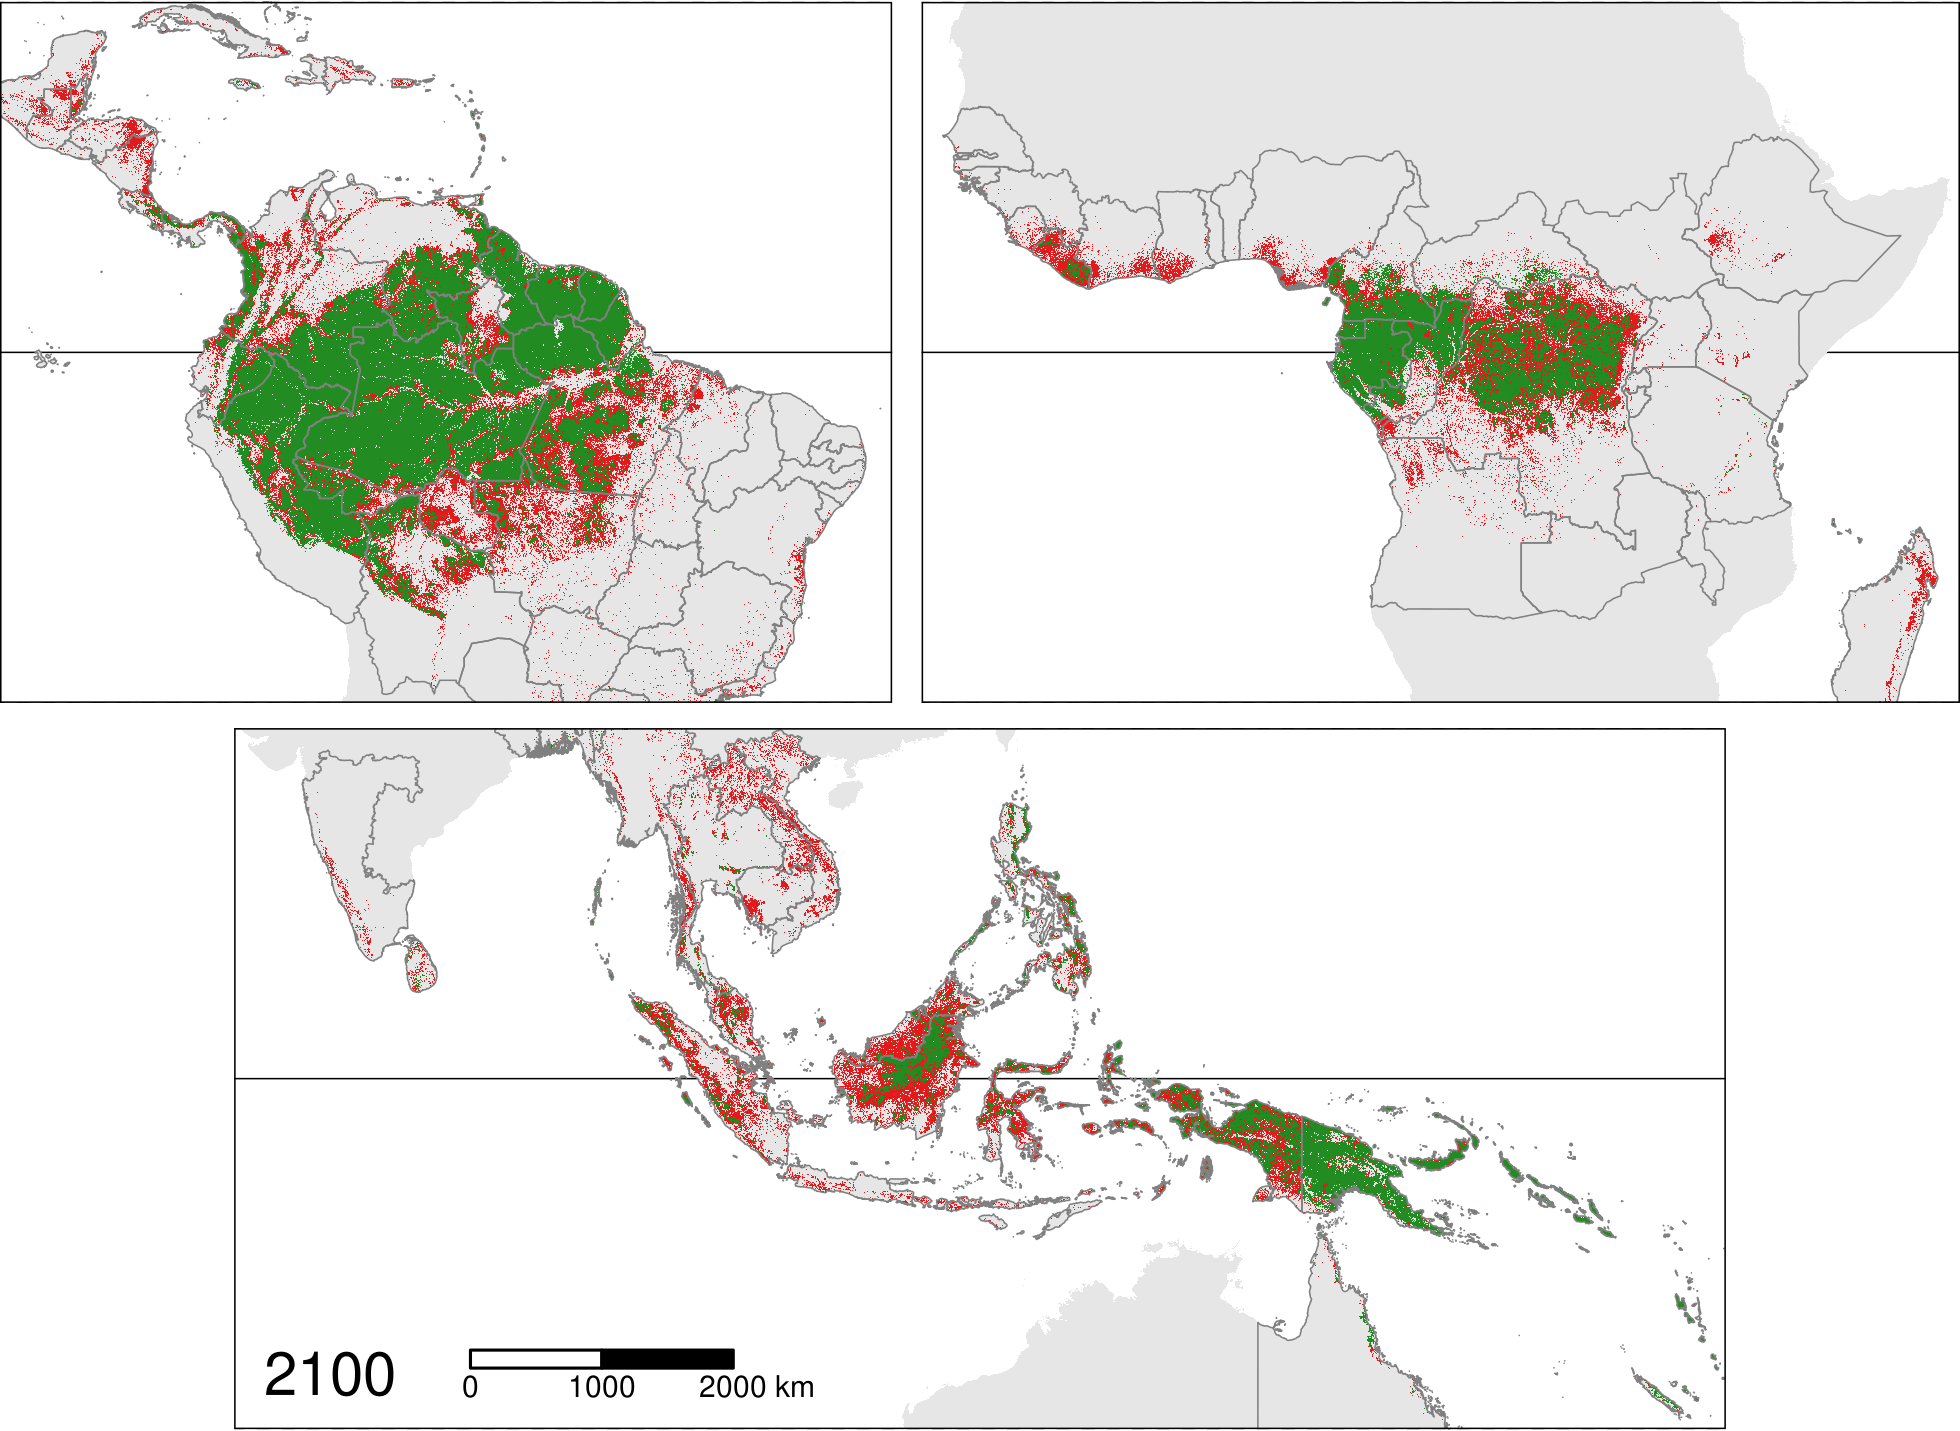
\includegraphics[width=\textwidth]{figs_article/fcc2100} 

}

\caption{\textbf{Pantropical map of the predicted change in forest cover}. Maps show the predicted change in tropical moist forest cover in the three continents (America, Africa, and Asia) for the period 2020--2100 under a business-as-usual scenario of deforestation. The horizontal black line represents the Equator. The boundaries of the study area are represented by dark grey lines. For the deforestation projections, we assumed no diffusion of the deforestation between countries. Forest areas in \textcolor{red}{red} are predicted to be deforested in the period 2020--2100, while forest areas in \textcolor{darkgreen}{green} are likely to still exist in 2100. Several countries on the three continents are expected to lose all their tropical moist forest by 2100 (including Nicaragua and Mexico in Central America, Madagascar and Ghana in Africa, and Laos and Vietnam in Asia). We predict progressive fragmentation of the remaining forest in the future, with an increasing number of isolated forest patches of smaller size (e.g.~Pará state in Brazil, the Democratic Republic of the Congo, and Indonesia). These maps make it possible to identify both future hotspots of deforestation and forest refuge areas (e.g.~concentrated in the heart of the Amazon, West Central Africa, and Papua New Guinea). An interactive map is available at \url{https://forestatrisk.cirad.fr/maps.html}, and a zoom of this map for the DRC is available in Supplementary Materials.}\label{fig:fcc2100}
\end{figure}



\begin{figure}[H]

{\centering 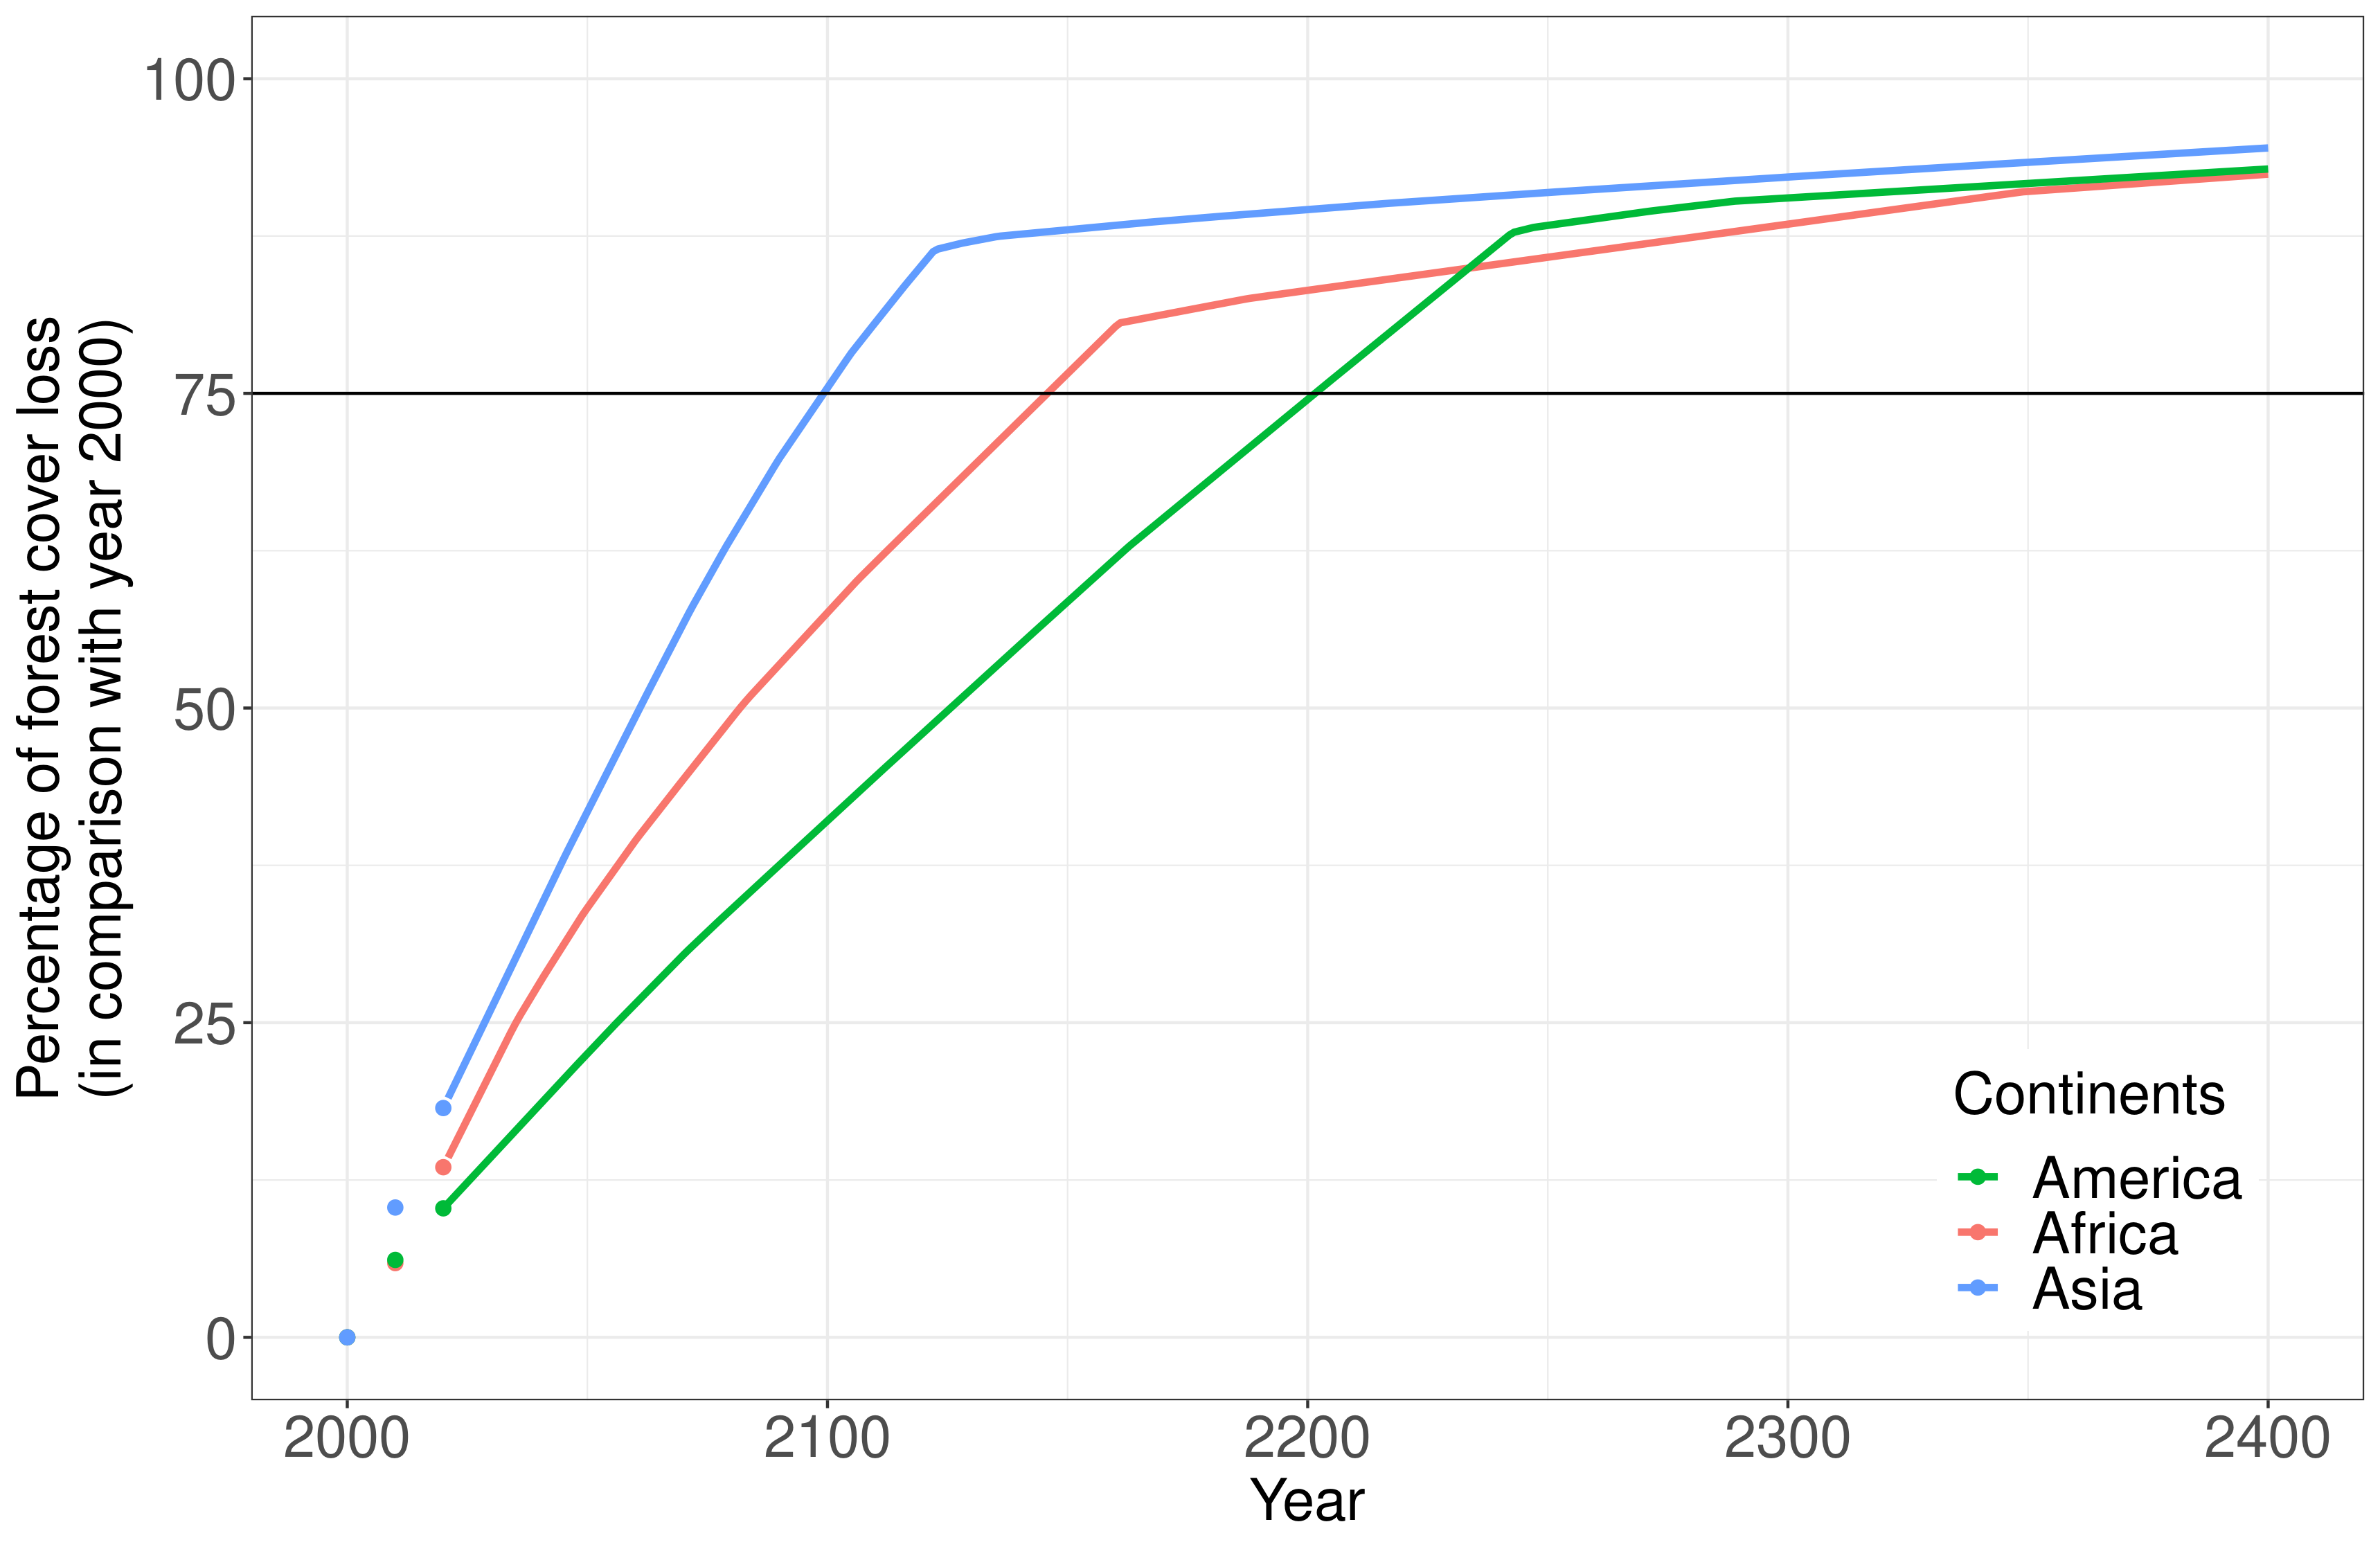
\includegraphics[width=\textwidth]{figs_article/perc_loss_cont} 

}

\caption{\textbf{Projected percentage of forest cover loss per continent}. Points represent the observed percentage of forest cover loss (in comparison with the year 2000) for the years 2000 (0\%), 2010, and 2020, for the three continents: America, Africa, and Asia. Lines represent the projected percentage of forest cover loss (in comparison with the year 2000) from year 2020 to 2400 per continent. For the deforestation projections, we assumed no diffusion of the deforestation between countries. When large countries with high annual deforested areas (Brazil for America, DRC for Africa, and Indonesia for Asia) have no more forest (in 2237, 2156, and 2115, respectively, see table~S16), deforestation at the continent scale is rapidly decreasing. The horizontal black line indicates a loss of 75\% of the forest cover in comparison with the year 2000. Under a ``business-as-usual'' scenario, this should happen in 2094, 2143, and 2197 for Asia, Africa, and America, respectively. The confidence envelopes around the mean are obtained using the lower and upper limits of the confidence intervals of the mean annual deforested areas for all study areas.}\label{fig:perc-loss}
\end{figure}



\begin{figure}[H]

{\centering 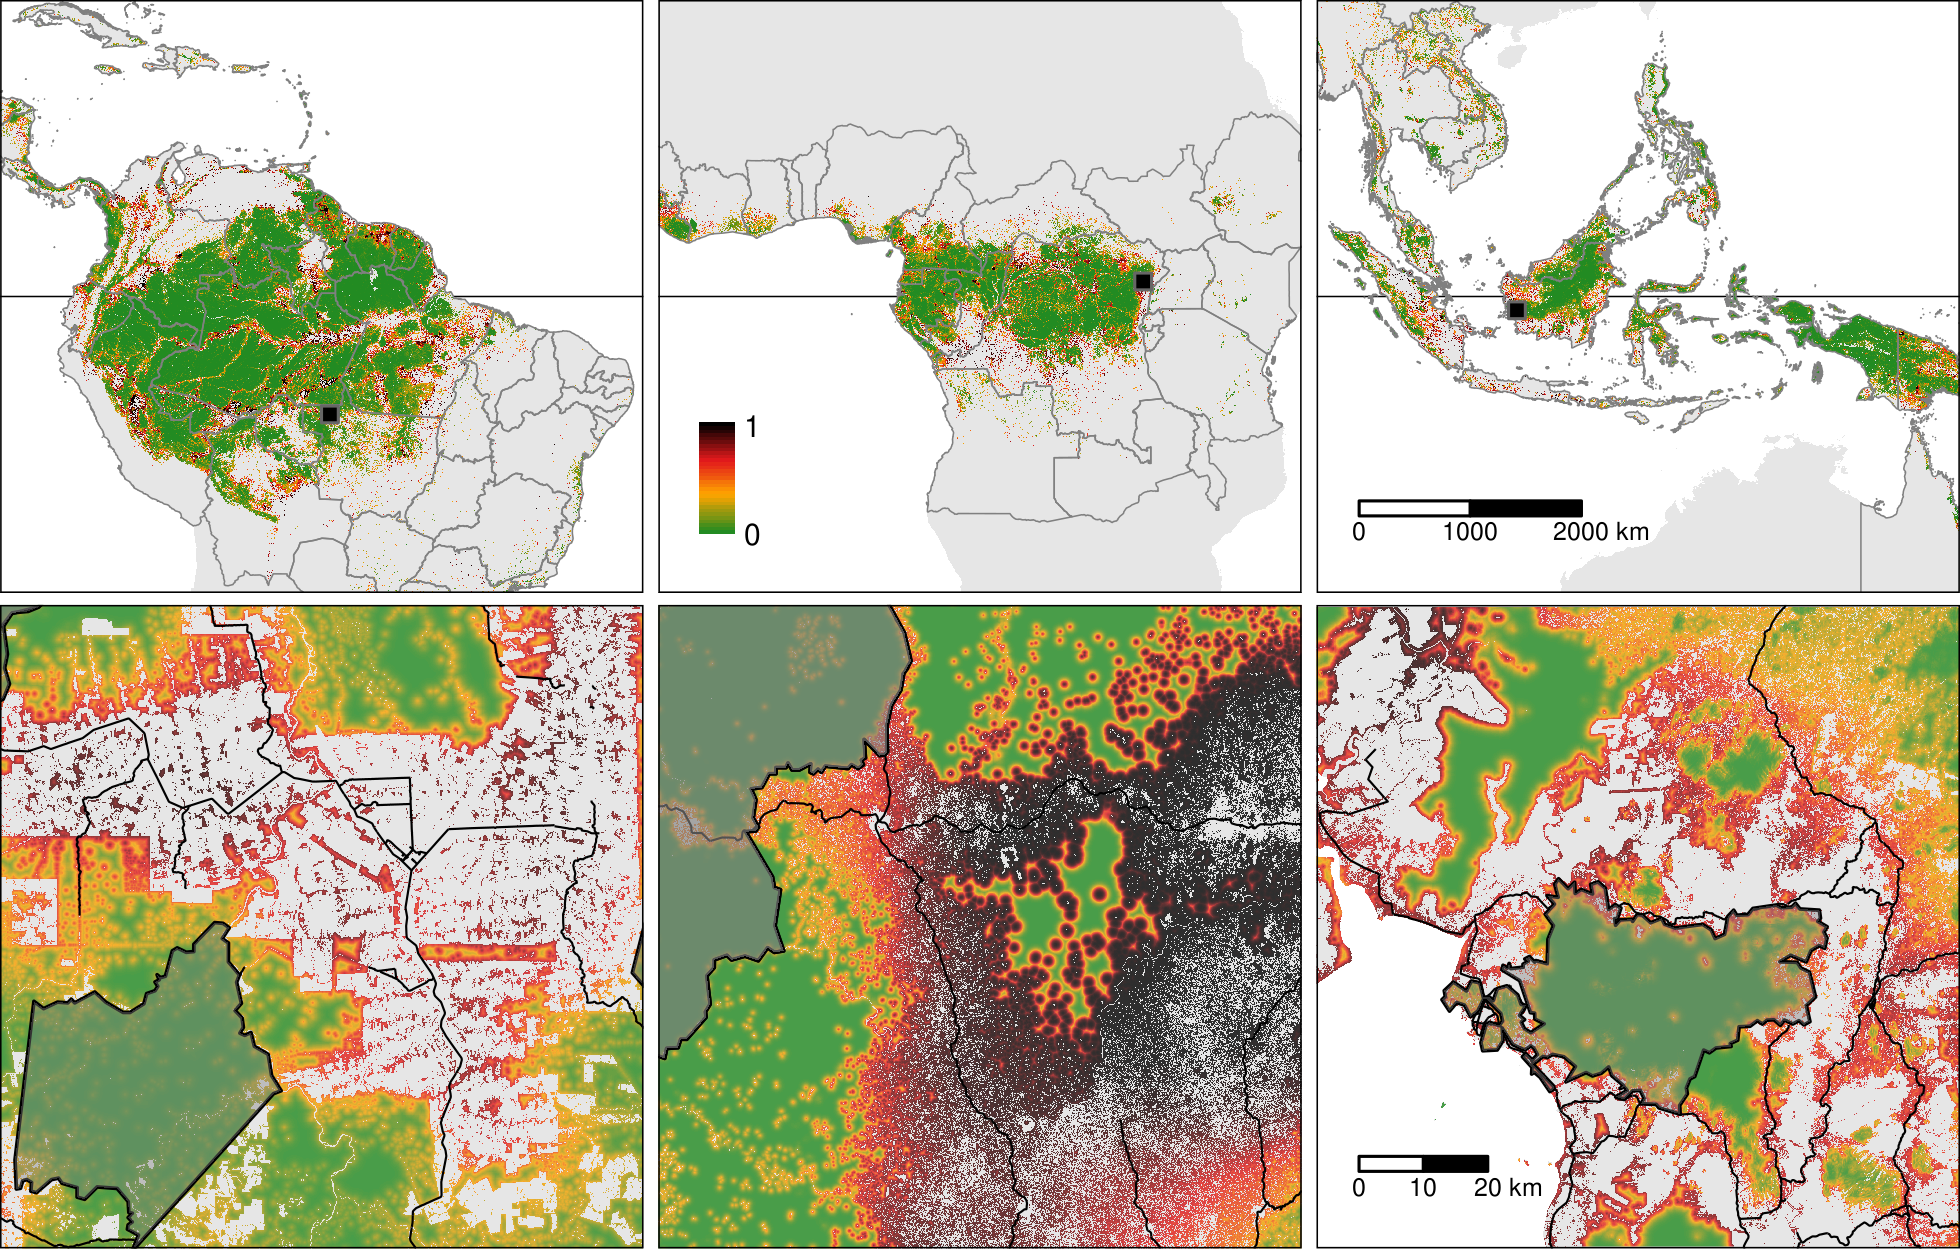
\includegraphics[width=\textwidth]{figs_article/prob_zoom} 

}

\caption{\textbf{Pantropical map of the risk of deforestation}. \emph{Upper panels}: Maps of the spatial probability of deforestation at 30~m resolution for the three continents. Maps of the spatial probability of deforestation at the level of the study area were aggregated at the pantropical level. The horizontal black line represents the Equator. The boundaries of the study area are represented by dark grey lines. Coloured pixels represent forest pixels for the year 2020. Inside each study area, forest areas in dark red have a higher risk of deforestation than forest areas in green. \emph{Lower panels}: Detailed maps for three 100 \(\times\) 100~km regions (black squares in the upper panels) in the Mato Grosso state (Brazil), the Albertine Rift mountains (the Democratic Republic of the Congo), and the West Kalimantan region (Borneo Indonesian part). Deforestation probability is lower inside protected areas (black shaded polygons) and increases when the forest is located at a distance closer to roads (dark grey lines) and forest edge. An interactive map of the spatial probability of deforestation is available at \url{https://forestatrisk.cirad.fr/maps.html}.}\label{fig:prob}
\end{figure}



\begin{figure}[H]

{\centering 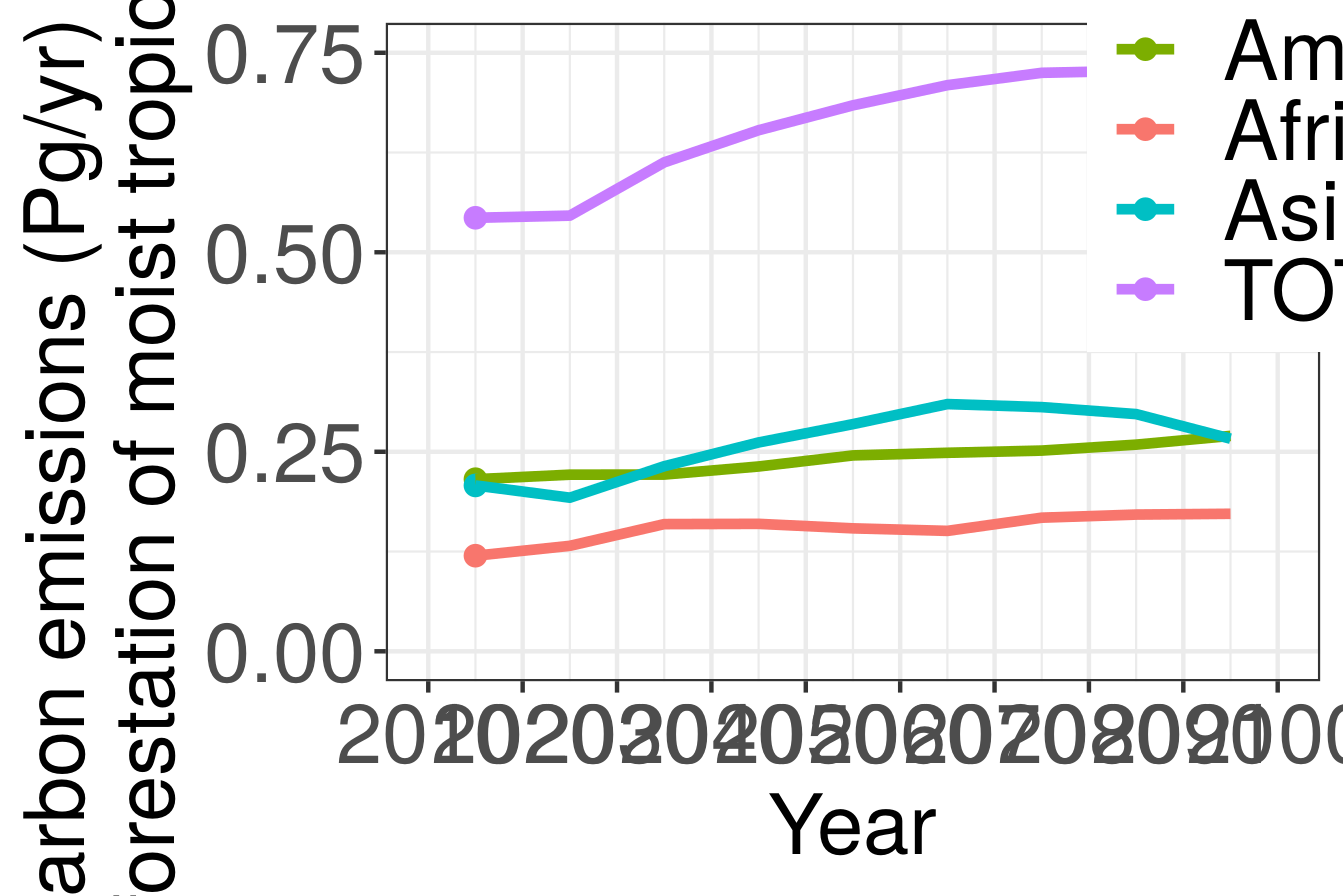
\includegraphics[width=\textwidth]{figs_article/C_trend} 

}

\caption{\textbf{Aboveground carbon emissions associated with projected deforestation}. This figure shows the changes in annual carbon emissions (Pg/yr) associated with the predicted deforestation of moist tropical forests. Mean annual carbon emissions are computed for ten-year intervals from 2010--2020 to 2090--2100. The dots represent the observed mean annual carbon emissions (based on past deforestation maps) for the period 2010--2020, for the three continents (America, Africa, and Asia), and for the three continents combined. Lines represent the projected mean annual carbon emissions based on projected forest cover change maps from 2020--2030 to 2090--2100 per continent, and for all continents together. The confidence envelopes around the mean are obtained using the lower and upper limits of the confidence intervals of the mean annual deforested areas for all study areas. Annual carbon emissions at the pantropical scale are predicted to increase from 0.525~Pg/yr in 2010--2020 to 0.746~Pg/yr in 2070--2080, representing a 42\% increase (+0.221~Pg/yr).}\label{fig:c-em}
\end{figure}



\begin{figure}[H]

{\centering 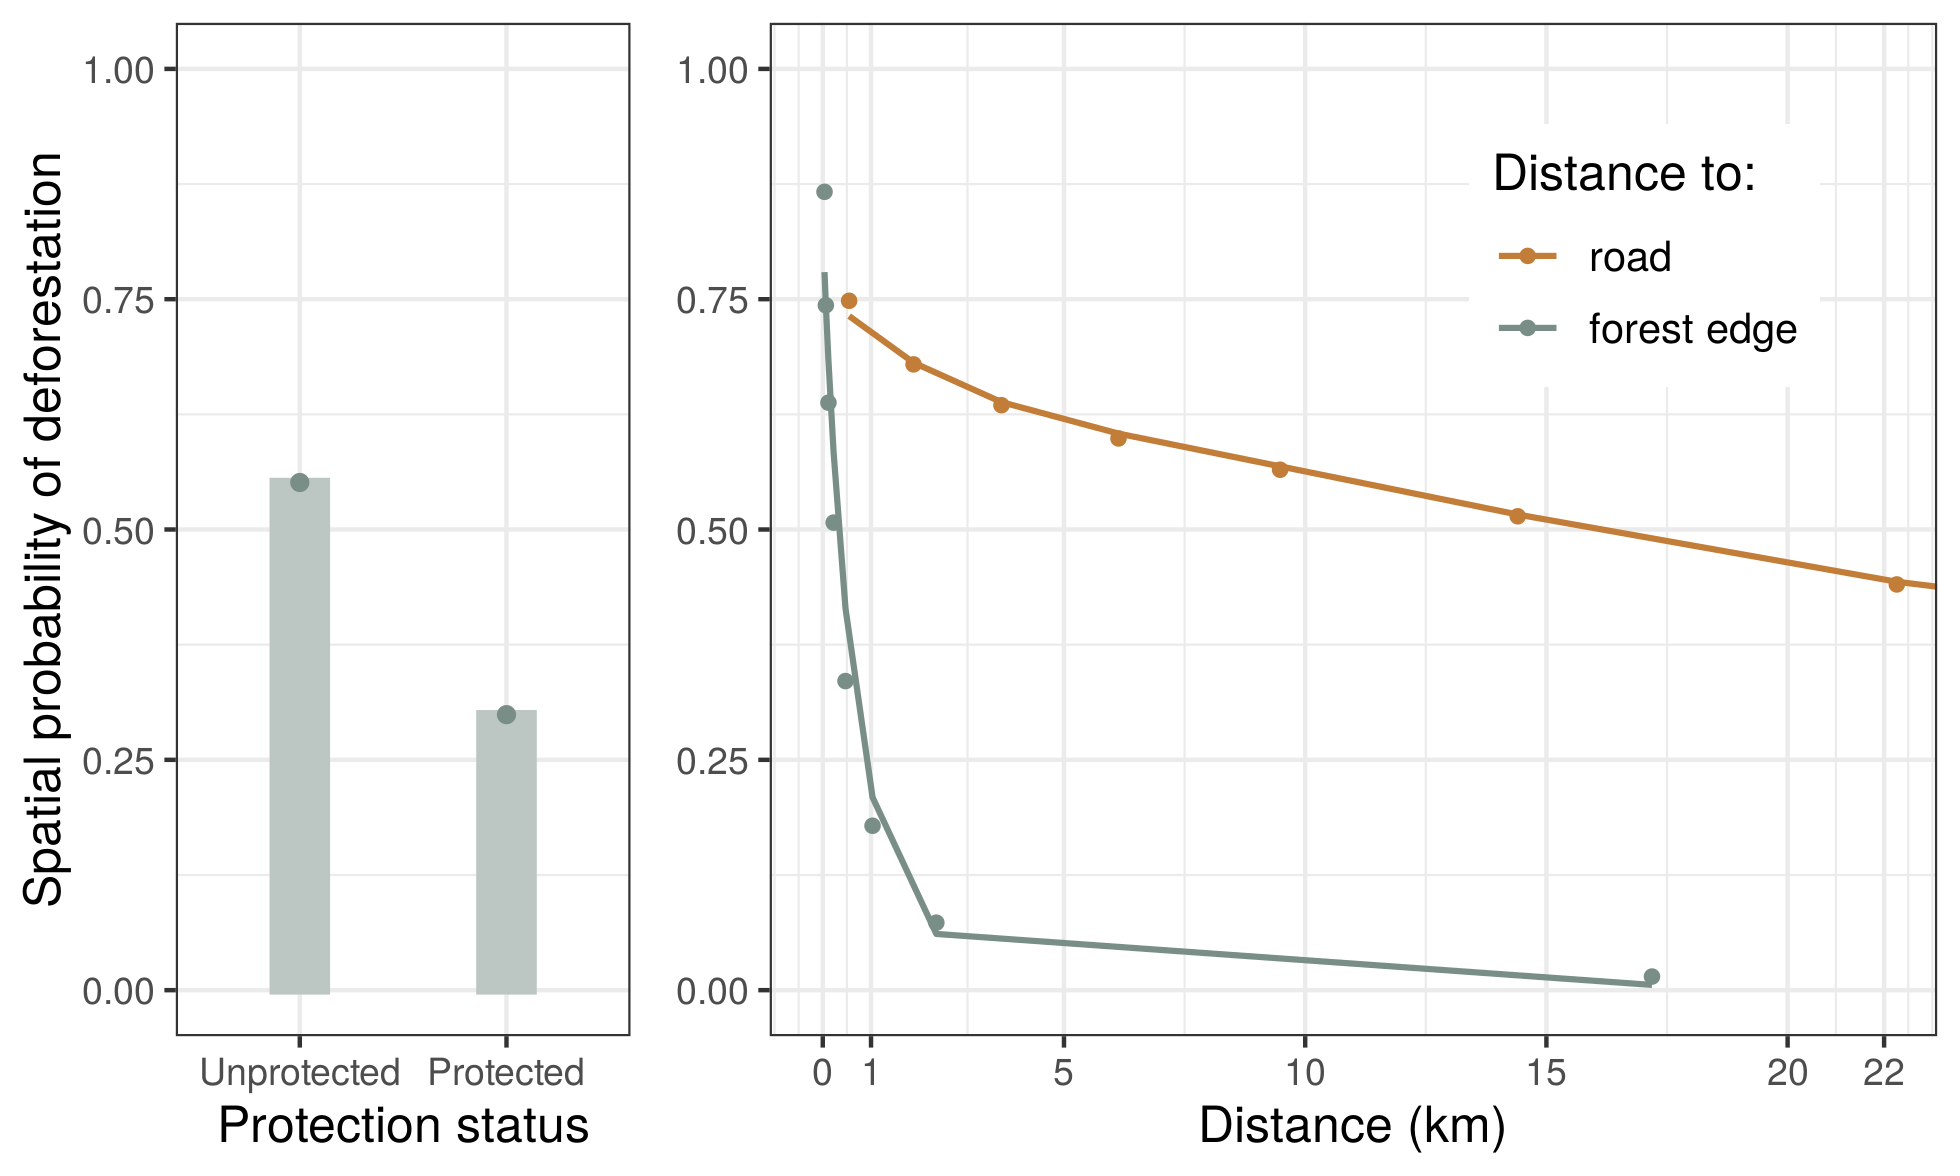
\includegraphics[width=\textwidth]{figs_article/proba-var} 

}

\caption{\textbf{Effects of protected areas, roads, and distance to forest edge on the spatial probability of deforestation}. In this figure, we use a representative dataset at the global scale where the number of observations for each study area is proportional to its forest cover in 2010. We used a total of 813,796 observations sampled in the original dataset (table~S3). \emph{Left}: The dots represent the observed mean probability of deforestation in each forest protection class, either protected or unprotected. Bars represent the mean of the predicted probabilities of deforestation obtained from the deforestation model for all observations in each class. \emph{Right}: The dots represent the local mean probability of deforestation for each bin of 10 percentiles for the distance. Lines represent the mean of the predicted probabilities of deforestation obtained from the deforestation model for all observations in each bin. Note that for distance to forest edge, the first dot accounts for three bins while for distance to road, bins for a distance \textgreater~23~km are not shown. For both left and right panels, confidence intervals for predictions were to small to be represented because of the high number of observations per class and bin.}\label{fig:proba-var}
\end{figure}

\newpage

\hypertarget{tables}{%
\section*{Tables}\label{tables}}
\addcontentsline{toc}{section}{Tables}



\begin{table}[H]

\caption{\label{tab:fcc}\textbf{Past and predicted changes in forest cover}. We provide past and predicted forest cover for the three continents and for the three countries with the highest forest cover in 2010 for each continent (Brazil in America, the DRC in Africa, and Indonesia in Asia). Past forest cover areas (in thousand hectares, Kha) refers to their status on January 1\textsuperscript{st} 2000, 2010, and 2020 (``fc2000'', ``fc2010'', and ``fc2020'', respectively). We provide the mean annual deforested area \(d\) (Kha/yr) for the last ten-year period from January 1\textsuperscript{st} 2009 to January 1\textsuperscript{st} 2019 (deforestation in 2019 is not included, see Methods), and the corresponding mean annual deforestation rate \(p\) (\%/yr). Projected forest cover areas are given for the years 2050 and 2100 (``fc2050'' and ``fc2100''). Projections are based on the forest cover in 2020 (``fc2020'') and the mean annual deforested area (\(d\)) assuming a business-as-usual scenario of deforestation. Column ``loss21'' indicates the projected percentage of forest cover loss during the 21\textsuperscript{st} century (2100 vs.~2000). We estimate the year (``yr75'') at which 75\% of the forest cover in 2000 will have disappeared.\vspace{0.5cm}}
\centering
\fontsize{10}{12}\selectfont
\begin{tabular}[t]{lrrrrrrrrr}
\toprule
\multicolumn{1}{l}{Regions} & \multicolumn{1}{r}{fc2000} & \multicolumn{1}{r}{fc2010} & \multicolumn{1}{r}{fc2020} & \multicolumn{1}{r}{$d$} & \multicolumn{1}{r}{$p$} & \multicolumn{1}{r}{fc2050} & \multicolumn{1}{r}{fc2100} & \multicolumn{1}{r}{loss21} & \multicolumn{1}{r}{yr75} \\
 & (Kha) & (Kha) & (Kha) & (Kha/yr) & (\%/yr) & (Kha) & (Kha) & (\%) & \\
\midrule
\addlinespace[0.3em]
\multicolumn{10}{l}{\textbf{Countries}}\\
\cellcolor{gray!6}{\hspace{1em}Brazil} & \cellcolor{gray!6}{375,893} & \cellcolor{gray!6}{349,784} & \cellcolor{gray!6}{334,982} & \cellcolor{gray!6}{1,537} & \cellcolor{gray!6}{0.4} & \cellcolor{gray!6}{288,862} & \cellcolor{gray!6}{211,996} & \cellcolor{gray!6}{44} & \cellcolor{gray!6}{2183}\\
\hspace{1em}DRC & 131,621 & 126,164 & 117,812 & 860 & 0.7 & 92,007 & 48,999 & 63 & 2114\\
\cellcolor{gray!6}{\hspace{1em}Indonesia} & \cellcolor{gray!6}{141,262} & \cellcolor{gray!6}{127,699} & \cellcolor{gray!6}{116,317} & \cellcolor{gray!6}{1,215} & \cellcolor{gray!6}{1.0} & \cellcolor{gray!6}{79,853} & \cellcolor{gray!6}{19,078} & \cellcolor{gray!6}{86} & \cellcolor{gray!6}{2087}\\
\addlinespace[0.3em]
\multicolumn{10}{l}{\textbf{Continents}}\\
\hspace{1em}America & 690,358 & 648,928 & 621,160 & 2,893 & 0.5 & 534,552 & 404,344 & 41 & 2197\\
\cellcolor{gray!6}{\hspace{1em}Africa} & \cellcolor{gray!6}{275,745} & \cellcolor{gray!6}{259,667} & \cellcolor{gray!6}{238,791} & \cellcolor{gray!6}{2,176} & \cellcolor{gray!6}{0.9} & \cellcolor{gray!6}{180,848} & \cellcolor{gray!6}{115,591} & \cellcolor{gray!6}{58} & \cellcolor{gray!6}{2143}\\
\hspace{1em}Asia & 301,412 & 270,679 & 246,894 & 2,533 & 1.0 & 171,417 & 66,034 & 78 & 2094\\
\cellcolor{gray!6}{\hspace{1em}All cont.} & \cellcolor{gray!6}{1,267,515} & \cellcolor{gray!6}{1,179,273} & \cellcolor{gray!6}{1,106,845} & \cellcolor{gray!6}{7,602} & \cellcolor{gray!6}{0.7} & \cellcolor{gray!6}{886,816} & \cellcolor{gray!6}{585,968} & \cellcolor{gray!6}{54} & \cellcolor{gray!6}{2171}\\
\bottomrule
\end{tabular}
\end{table}

\newpage

%% =========================================================================================
%% REFERENCES
%% =========================================================================================

\hypertarget{references}{%
\section*{References}\label{references}}
\addcontentsline{toc}{section}{References}

  %%\bibliography{/home/ghislain/Documents/Bibliography/biblio.bib}

\begin{thebibliography}{99}
\expandafter\ifx\csname url\endcsname\relax
  \def\url#1{\texttt{#1}}\fi
\expandafter\ifx\csname urlprefix\endcsname\relax\def\urlprefix{URL }\fi
\providecommand{\bibinfo}[2]{#2}
\providecommand{\eprint}[2][]{\url{#2}}

\bibitem{IPCC2014}
\bibinfo{author}{{IPCC}}.
\newblock \bibinfo{title}{{Climate Change 2014: Synthesis Report. Contribution
  of Working Groups I, II and III to the Fifth Assessment Report of the
  Intergovernmental Panel on Climate Change}}.
\newblock \bibinfo{type}{Tech. Rep.}, \bibinfo{institution}{The
  Intergovernmental Panel on Climate Change, IPCC} (\bibinfo{year}{2014}).

\bibitem{Cardinale2012}
\bibinfo{author}{Cardinale, B.~J.} \emph{et~al.}
\newblock \bibinfo{title}{Biodiversity loss and its impact on humanity}.
\newblock \emph{\bibinfo{journal}{Nature}} \textbf{\bibinfo{volume}{486}},
  \bibinfo{pages}{59--67} (\bibinfo{year}{2012}).

\bibitem{Gibson2011}
\bibinfo{author}{Gibson, L.} \emph{et~al.}
\newblock \bibinfo{title}{Primary forests are irreplaceable for sustaining
  tropical biodiversity}.
\newblock \emph{\bibinfo{journal}{Nature}} \textbf{\bibinfo{volume}{478}},
  \bibinfo{pages}{378--381} (\bibinfo{year}{2011}).
%\newblock \urlprefix\url{http://dx.doi.org/10.1038/nature10425}.

\bibitem{Wilson2012}
\bibinfo{author}{Wilson, J.~B.}, \bibinfo{author}{Peet, R.~K.},
  \bibinfo{author}{Dengler, J.} \& \bibinfo{author}{Pärtel, M.}
\newblock \bibinfo{title}{Plant species richness: the world records}.
\newblock \emph{\bibinfo{journal}{Journal of Vegetation Science}}
  \textbf{\bibinfo{volume}{23}}, \bibinfo{pages}{796--802}
  (\bibinfo{year}{2012}).
%\newblock
%  \urlprefix\url{https://onlinelibrary.wiley.com/doi/abs/10.1111/j.1654-1103.2012.01400.x}.

\bibitem{Baccini2017}
\bibinfo{author}{Baccini, A.} \emph{et~al.}
\newblock \bibinfo{title}{Tropical forests are a net carbon source based on
  aboveground measurements of gain and loss}.
\newblock \emph{\bibinfo{journal}{Science}} \textbf{\bibinfo{volume}{358}},
  \bibinfo{pages}{230--234} (\bibinfo{year}{2017}).
%\newblock \urlprefix\url{https://doi.org/10.1126/science.aam5962}.

\bibitem{Tollefson2020}
\bibinfo{author}{Tollefson, J.}
\newblock \bibinfo{title}{Why deforestation and extinctions make pandemics more
  likely}.
\newblock \emph{\bibinfo{journal}{Nature}} \textbf{\bibinfo{volume}{584}},
  \bibinfo{pages}{175--176} (\bibinfo{year}{2020}).
%\newblock \urlprefix\url{https://doi.org/10.1038/d41586-020-02341-1}.

\bibitem{Dickinson1992}
\bibinfo{author}{Dickinson, R.~E.} \& \bibinfo{author}{Kennedy, P.}
\newblock \bibinfo{title}{Impacts on regional climate of {A}mazon
  deforestation}.
\newblock \emph{\bibinfo{journal}{Geophysical Research Letters}}
  \textbf{\bibinfo{volume}{19}}, \bibinfo{pages}{1947--1950}
  (\bibinfo{year}{1992}).
% \newblock
%   \urlprefix\url{https://agupubs.onlinelibrary.wiley.com/doi/abs/10.1029/92GL01905}.
% \newblock
%   \eprint{https://agupubs.onlinelibrary.wiley.com/doi/pdf/10.1029/92GL01905}.

\bibitem{Ellison2017}
\bibinfo{author}{Ellison, D.} \emph{et~al.}
\newblock \bibinfo{title}{Trees, forests and water: cool insights for a hot
  world}.
\newblock \emph{\bibinfo{journal}{Global Environmental Change}}
  \textbf{\bibinfo{volume}{43}}, \bibinfo{pages}{51 -- 61}
  (\bibinfo{year}{2017}).
% \newblock
%   \urlprefix\url{http://www.sciencedirect.com/science/article/pii/S0959378017300134}.

\bibitem{Zhang2021}
\bibinfo{author}{Zhang, M.} \& \bibinfo{author}{Wei, X.}
\newblock \bibinfo{title}{Deforestation, forestation, and water supply}.
\newblock \emph{\bibinfo{journal}{Science}} \textbf{\bibinfo{volume}{371}},
  \bibinfo{pages}{990--991} (\bibinfo{year}{2021}).
%\newblock \urlprefix\url{https://science.sciencemag.org/content/371/6533/990}.
% \newblock
%   \eprint{https://science.sciencemag.org/content/371/6533/990.full.pdf}.

\bibitem{Bradshaw2007}
\bibinfo{author}{Bradshaw, C. J.~A.}, \bibinfo{author}{Sodhi, N.~S.},
  \bibinfo{author}{Peh, K. S. .~H.} \& \bibinfo{author}{Brook, B.~W.}
\newblock \bibinfo{title}{Global evidence that deforestation amplifies flood
  risk and severity in the developing world}.
\newblock \emph{\bibinfo{journal}{Global Change Biology}}
  \textbf{\bibinfo{volume}{13}}, \bibinfo{pages}{2379--2395}
  (\bibinfo{year}{2007}).

\bibitem{FAO2015}
\bibinfo{author}{FAO}.
\newblock \bibinfo{title}{{Global Forest Resources Assessment 2015}}.
\newblock \bibinfo{type}{Tech. Rep.}, \bibinfo{institution}{Food and
  Agriculture Organization of the United Nations} (\bibinfo{year}{2015}).
% \newblock
%   \urlprefix\url{http://www.fao.org/fileadmin/user_upload/FRA/spreadsheet/FRA_data/BULK.zip}.

\bibitem{Hansen2013}
\bibinfo{author}{Hansen, M.~C.} \emph{et~al.}
\newblock \bibinfo{title}{High-resolution global maps of 21st-century forest
  cover change}.
\newblock \emph{\bibinfo{journal}{Science}} \textbf{\bibinfo{volume}{342}},
  \bibinfo{pages}{850--853} (\bibinfo{year}{2013}).
% \newblock
%   \urlprefix\url{http://www.sciencemag.org/content/342/6160/850.abstract}.
% \newblock \eprint{http://www.sciencemag.org/content/342/6160/850.full.pdf}.

\bibitem{Vancutsem2021}
\bibinfo{author}{Vancutsem, C.} \emph{et~al.}
\newblock \bibinfo{title}{Long-term (1990--2019) monitoring of forest cover
  changes in the humid tropics}.
\newblock \emph{\bibinfo{journal}{Science Advances}}
  \textbf{\bibinfo{volume}{7}} (\bibinfo{year}{2021}).
% \newblock
%   \urlprefix\url{https://advances.sciencemag.org/content/7/10/eabe1603}.
% \newblock
%   \eprint{https://advances.sciencemag.org/content/7/10/eabe1603.full.pdf}.

\bibitem{Achard2014}
\bibinfo{author}{Achard, F.} \emph{et~al.}
\newblock \bibinfo{title}{Determination of tropical deforestation rates and
  related carbon losses from 1990 to 2010}.
\newblock \emph{\bibinfo{journal}{Global Change Biology}}
  \textbf{\bibinfo{volume}{20}}, \bibinfo{pages}{2540--2554}
  (\bibinfo{year}{2014}).
%\newblock \urlprefix\url{http://dx.doi.org/10.1111/gcb.12605}.

\bibitem{Curtis2018}
\bibinfo{author}{Curtis, P.~G.}, \bibinfo{author}{Slay, C.~M.},
  \bibinfo{author}{Harris, N.~L.}, \bibinfo{author}{Tyukavina, A.} \&
  \bibinfo{author}{Hansen, M.~C.}
\newblock \bibinfo{title}{Classifying drivers of global forest loss}.
\newblock \emph{\bibinfo{journal}{Science}} \textbf{\bibinfo{volume}{361}},
  \bibinfo{pages}{1108--1111} (\bibinfo{year}{2018}).
%\newblock \urlprefix\url{https://doi.org/10.1126/science.aau3445}.

\bibitem{Geist2002}
\bibinfo{author}{Geist, H.~J.} \& \bibinfo{author}{Lambin, E.~F.}
\newblock \bibinfo{title}{Proximate causes and underlying driving forces of
  tropical deforestation}.
\newblock \emph{\bibinfo{journal}{{BioScience}}} \textbf{\bibinfo{volume}{52}},
  \bibinfo{pages}{143} (\bibinfo{year}{2002}).
% \newblock
%   \urlprefix\url{https://doi.org/10.1641/0006-3568(2002)052[0143:pcaudf]2.0.co;2}.

\bibitem{Clark2001}
\bibinfo{author}{Clark, J.~S.} \emph{et~al.}
\newblock \bibinfo{title}{{Ecological forecasts: an emerging imperative}}.
\newblock \emph{\bibinfo{journal}{Science}} \textbf{\bibinfo{volume}{293}},
  \bibinfo{pages}{657--660} (\bibinfo{year}{2001}).

\bibitem{Pereira2020}
\bibinfo{author}{Pereira, H.~M.} \emph{et~al.}
\newblock \bibinfo{title}{Global trends in biodiversity and ecosystem services
  from 1900 to 2050}.
\newblock \emph{\bibinfo{journal}{bioRxiv}}
  \textbf{\bibinfo{volume}{2020.04.14.031716}} (\bibinfo{year}{2020}).
%\newblock \urlprefix\url{https://doi.org/10.1101/2020.04.14.031716}.

\bibitem{Goetz2015}
\bibinfo{author}{Goetz, S.~J.} \emph{et~al.}
\newblock \bibinfo{title}{Measurement and monitoring needs, capabilities and
  potential for addressing reduced emissions from deforestation and forest
  degradation under {REDD}+}.
\newblock \emph{\bibinfo{journal}{Environmental Research Letters}}
  \textbf{\bibinfo{volume}{10}}, \bibinfo{pages}{123001}
  (\bibinfo{year}{2015}).
%\newblock \urlprefix\url{https://doi.org/10.1088/1748-9326/10/12/123001}.

\bibitem{Avitabile2016}
\bibinfo{author}{Avitabile, V.} \emph{et~al.}
\newblock \bibinfo{title}{An integrated pan-tropical biomass map using multiple
  reference datasets}.
\newblock \emph{\bibinfo{journal}{Global Change Biology}}
  \textbf{\bibinfo{volume}{22}}, \bibinfo{pages}{1406--1420}
  (\bibinfo{year}{2016}).
%\newblock \urlprefix\url{https://doi.org/10.1111/gcb.13139}.

\bibitem{Kremen2008}
\bibinfo{author}{Kremen, C.} \emph{et~al.}
\newblock \bibinfo{title}{Aligning conservation priorities across taxa in
  {M}adagascar with high-resolution planning tools}.
\newblock \emph{\bibinfo{journal}{Science}} \textbf{\bibinfo{volume}{320}},
  \bibinfo{pages}{222--226} (\bibinfo{year}{2008}).

\bibitem{Mittermeier2011}
\bibinfo{author}{Mittermeier, R.~A.}, \bibinfo{author}{Turner, W.~R.},
  \bibinfo{author}{Larsen, F.~W.}, \bibinfo{author}{Brooks, T.~M.} \&
  \bibinfo{author}{Gascon, C.}
\newblock \bibinfo{title}{Global biodiversity conservation: the critical role
  of hotspots}.
\newblock In \emph{\bibinfo{booktitle}{Biodiversity Hotspots}},
  \bibinfo{pages}{3--22} (\bibinfo{publisher}{Springer Berlin Heidelberg},
  \bibinfo{year}{2011}).
%\newblock \urlprefix\url{https://doi.org/10.1007/978-3-642-20992-5_1}.

\bibitem{Rosa2014}
\bibinfo{author}{Rosa, I.~M.}, \bibinfo{author}{Purves, D.},
  \bibinfo{author}{Carreiras, J.~M.} \& \bibinfo{author}{Ewers, R.~M.}
\newblock \bibinfo{title}{Modelling land cover change in the {B}razilian
  {A}mazon: temporal changes in drivers and calibration issues}.
\newblock \emph{\bibinfo{journal}{Regional Environmental Change}}
  \bibinfo{pages}{1--15} (\bibinfo{year}{2014}).

\bibitem{Laurance2014}
\bibinfo{author}{Laurance, W.~F.} \emph{et~al.}
\newblock \bibinfo{title}{A global strategy for road building}.
\newblock \emph{\bibinfo{journal}{Nature}} \textbf{\bibinfo{volume}{513}},
  \bibinfo{pages}{229--232} (\bibinfo{year}{2014}).
%\newblock \urlprefix\url{https://doi.org/10.1038/nature13717}.

\bibitem{Andam2008}
\bibinfo{author}{Andam, K.~S.}, \bibinfo{author}{Ferraro, P.~J.},
  \bibinfo{author}{Pfaff, A.}, \bibinfo{author}{Sanchez-Azofeifa, G.~A.} \&
  \bibinfo{author}{Robalino, J.~A.}
\newblock \bibinfo{title}{Measuring the effectiveness of protected area
  networks in reducing deforestation}.
\newblock \emph{\bibinfo{journal}{Proceedings of the National Academy of
  Sciences}} \textbf{\bibinfo{volume}{105}}, \bibinfo{pages}{16089--16094}
  (\bibinfo{year}{2008}).
%\newblock \urlprefix\url{https://doi.org/10.1073/pnas.0800437105}.

\bibitem{Wolf2021}
\bibinfo{author}{Wolf, C.}, \bibinfo{author}{Levi, T.},
  \bibinfo{author}{Ripple, W.~J.}, \bibinfo{author}{Z{\'{a}}rrate-Charry,
  D.~A.} \& \bibinfo{author}{Betts, M.~G.}
\newblock \bibinfo{title}{A forest loss report card for the world's protected
  areas}.
\newblock \emph{\bibinfo{journal}{Nature Ecology {\&} Evolution}} \textbf{\bibinfo{volume}{5}},
 \bibinfo{pages}{520--529} (\bibinfo{year}{2021}).
%\newblock \urlprefix\url{https://doi.org/10.1038/s41559-021-01389-0}.

\bibitem{Aguiar2016}
\bibinfo{author}{Aguiar, A. P.~D.} \emph{et~al.}
\newblock \bibinfo{title}{Land use change emission scenarios: anticipating a
  forest transition process in the brazilian amazon}.
\newblock \emph{\bibinfo{journal}{Global Change Biology}}
  \textbf{\bibinfo{volume}{22}}, \bibinfo{pages}{1821--1840}
  (\bibinfo{year}{2016}).
%\newblock \urlprefix\url{https://doi.org/10.1111/gcb.13134}.

\bibitem{Swann2015}
\bibinfo{author}{Swann, A.~L.}, \bibinfo{author}{Longo, M.},
  \bibinfo{author}{Knox, R.~G.}, \bibinfo{author}{Lee, E.} \&
  \bibinfo{author}{Moorcroft, P.~R.}
\newblock \bibinfo{title}{Future deforestation in the amazon and consequences
  for south american climate}.
\newblock \emph{\bibinfo{journal}{Agricultural and Forest Meteorology}}
  \textbf{\bibinfo{volume}{214-215}}, \bibinfo{pages}{12--24}
  (\bibinfo{year}{2015}).
%\newblock \urlprefix\url{https://doi.org/10.1016/j.agrformet.2015.07.006}.

\bibitem{Soares-Filho2006}
\bibinfo{author}{Soares-Filho, B.~S.} \emph{et~al.}
\newblock \bibinfo{title}{Modelling conservation in the {A}mazon basin}.
\newblock \emph{\bibinfo{journal}{Nature}} \textbf{\bibinfo{volume}{440}},
  \bibinfo{pages}{520--523} (\bibinfo{year}{2006}).
%\newblock \urlprefix\url{https://doi.org/10.1038/nature04389}.

\bibitem{Pimm2014}
\bibinfo{author}{Pimm, S.~L.} \emph{et~al.}
\newblock \bibinfo{title}{The biodiversity of species and their rates of
  extinction, distribution, and protection}.
\newblock \emph{\bibinfo{journal}{Science}} \textbf{\bibinfo{volume}{344}},
  \bibinfo{pages}{1246752--1246752} (\bibinfo{year}{2014}).
%\newblock \urlprefix\url{https://doi.org/10.1126/science.1246752}.

\bibitem{Vieilledent2016}
\bibinfo{author}{Vieilledent, G.} \emph{et~al.}
\newblock \bibinfo{title}{Bioclimatic envelope models predict a decrease in
  tropical forest carbon stocks with climate change in {M}adagascar}.
\newblock \emph{\bibinfo{journal}{Journal of Ecology}}
  \textbf{\bibinfo{volume}{104}}, \bibinfo{pages}{703--715}
  (\bibinfo{year}{2016}).
% \newblock
%   \urlprefix\url{https://besjournals.onlinelibrary.wiley.com/doi/abs/10.1111/1365-2745.12548}.
% \newblock
%   \eprint{https://besjournals.onlinelibrary.wiley.com/doi/pdf/10.1111/1365-2745.12548}.

\bibitem{Saatchi2011}
\bibinfo{author}{Saatchi, S.~S.} \emph{et~al.}
\newblock \bibinfo{title}{Benchmark map of forest carbon stocks in tropical
  regions across three continents}.
\newblock \emph{\bibinfo{journal}{Proceedings of the National Academy of
  Sciences}} \textbf{\bibinfo{volume}{108}}, \bibinfo{pages}{9899--9904}
  (\bibinfo{year}{2011}).
%\newblock \urlprefix\url{http://www.pnas.org/content/108/24/9899.abstract}.
%\newblock \eprint{http://www.pnas.org/content/108/24/9899.full.pdf+html}.

\bibitem{Dargie2017}
\bibinfo{author}{Dargie, G.~C.} \emph{et~al.}
\newblock \bibinfo{title}{Age, extent and carbon storage of the central {C}ongo
  {B}asin peatland complex}.
\newblock \emph{\bibinfo{journal}{Nature}} \textbf{\bibinfo{volume}{542}},
  \bibinfo{pages}{86--90} (\bibinfo{year}{2017}).
%\newblock \urlprefix\url{https://doi.org/10.1038/nature21048}.

\bibitem{Brinck2017}
\bibinfo{author}{Brinck, K.} \emph{et~al.}
\newblock \bibinfo{title}{High resolution analysis of tropical forest
  fragmentation and its impact on the global carbon cycle}.
\newblock \emph{\bibinfo{journal}{Nature Communications}}
  \textbf{\bibinfo{volume}{8}}, \bibinfo{pages}{14855} (\bibinfo{year}{2017}).
%\newblock \urlprefix\url{http://dx.doi.org/10.1038/ncomms14855}.

\bibitem{Harris2012}
\bibinfo{author}{Harris, N.~L.} \emph{et~al.}
\newblock \bibinfo{title}{Baseline map of carbon emissions from deforestation
  in tropical regions}.
\newblock \emph{\bibinfo{journal}{Science}} \textbf{\bibinfo{volume}{336}},
  \bibinfo{pages}{1573--1576} (\bibinfo{year}{2012}).
%\newblock \urlprefix\url{https://doi.org/10.1126/science.1217962}.

\bibitem{IPCC2019}
\bibinfo{author}{IPCC}.
\newblock \bibinfo{title}{{Refinement to the 2006 IPCC Guidelines for National
  Greenhouse Gas Inventories. Volume 4. Agriculture, Forestry and Other Land
  Use}}.
\newblock \bibinfo{type}{Tech. Rep.}, \bibinfo{institution}{The
  Intergovernmental Panel on Climate Change, IPCC/IGES},
  \bibinfo{address}{Japan} (\bibinfo{year}{2019}).
% \newblock
%   \urlprefix\url{https://www.ipcc-nggip.iges.or.jp/public/2019rf/vol4.html}.

\bibitem{Bruner2001}
\bibinfo{author}{Bruner, A.~G.}
\newblock \bibinfo{title}{Effectiveness of parks in protecting tropical
  biodiversity}.
\newblock \emph{\bibinfo{journal}{Science}} \textbf{\bibinfo{volume}{291}},
  \bibinfo{pages}{125--128} (\bibinfo{year}{2001}).
%\newblock \urlprefix\url{https://doi.org/10.1126/science.291.5501.125}.

\bibitem{Cazalis2020}
\bibinfo{author}{Cazalis, V.} \emph{et~al.}
\newblock \bibinfo{title}{Effectiveness of protected areas in conserving
  tropical forest birds}.
\newblock \emph{\bibinfo{journal}{Nature Communications}}
  \textbf{\bibinfo{volume}{11}} (\bibinfo{year}{2020}).
%\newblock \urlprefix\url{https://doi.org/10.1038/s41467-020-18230-0}.

\bibitem{Yang2021}
\bibinfo{author}{Yang, H.} \emph{et~al.}
\newblock \bibinfo{title}{A global assessment of the impact of individual
  protected areas on preventing forest loss}.
\newblock \emph{\bibinfo{journal}{Science of The Total Environment}}
  \bibinfo{pages}{145995} (\bibinfo{year}{2021}).
%\newblock \urlprefix\url{https://doi.org/10.1016/j.scitotenv.2021.145995}.

\bibitem{Schleicher2019}
\bibinfo{author}{Schleicher, J.} \emph{et~al.}
\newblock \bibinfo{title}{Statistical matching for conservation science}.
\newblock \emph{\bibinfo{journal}{Conservation Biology}}
  \textbf{\bibinfo{volume}{34}}, \bibinfo{pages}{538--549}
  (\bibinfo{year}{2019}).
%\newblock \urlprefix\url{https://doi.org/10.1111/cobi.13448}.

\bibitem{Barnes1990}
\bibinfo{author}{Barnes, R. F.~W.}
\newblock \bibinfo{title}{Deforestation trends in tropical africa}.
\newblock \emph{\bibinfo{journal}{African Journal of Ecology}}
  \textbf{\bibinfo{volume}{28}}, \bibinfo{pages}{161--173}
  (\bibinfo{year}{1990}).
%\newblock \urlprefix\url{https://doi.org/10.1111/j.1365-2028.1990.tb01150.x}.

\bibitem{Soares-Filho2014}
\bibinfo{author}{Soares-Filho, B.} \emph{et~al.}
\newblock \bibinfo{title}{Cracking {B}razil's forest code}.
\newblock \emph{\bibinfo{journal}{Science}} \textbf{\bibinfo{volume}{344}},
  \bibinfo{pages}{363--364} (\bibinfo{year}{2014}).
%\newblock \urlprefix\url{https://doi.org/10.1126/science.1246663}.

\bibitem{Ribeiro2005}
\bibinfo{author}{Ribeiro, B.}, \bibinfo{author}{Veríssimo, A.} \&
  \bibinfo{author}{Pereira, K.}
\newblock \bibinfo{title}{O avanço do desmatamento sobre as \'areas protegidas
  em {R}ondônia}.
\newblock \emph{\bibinfo{journal}{O Estado da Amazônia (IMAZON)}}
  \textbf{\bibinfo{volume}{5}}, \bibinfo{pages}{1--5} (\bibinfo{year}{2005}).
%\newblock \urlprefix\url{https://www.imazon.org.br}.

\bibitem{Sangne2015}
\bibinfo{author}{Sangne, C.~Y.}, \bibinfo{author}{Barima, Y.~S.~S.},
  \bibinfo{author}{Bamba, I.} \& \bibinfo{author}{N'Doum{\'{e}}, C.-T.~A.}
\newblock \bibinfo{title}{Dynamique foresti{\`{e}}re post-conflits arm{\'{e}}s
  de la {F}or{\^{e}}t class{\'{e}}e du {H}aut-{S}assandra ({C}{\^{o}}te
  d'{I}voire)}.
\newblock \emph{\bibinfo{journal}{{VertigO}}}  (\bibinfo{year}{2015}).
%\newblock \urlprefix\url{https://doi.org/10.4000/vertigo.16784}.

\bibitem{Vieilledent2020}
\bibinfo{author}{Vieilledent, G.} \emph{et~al.}
\newblock \bibinfo{title}{It's not just poverty: unregulated global market and
  bad governance explain unceasing deforestation in {W}estern {M}adagascar}.
\newblock \emph{\bibinfo{journal}{bioRxiv}}
  \textbf{\bibinfo{volume}{2020.07.30.229104}} (\bibinfo{year}{2020}).
%\newblock \urlprefix\url{https://doi.org/10.1101/2020.07.30.229104}.

\bibitem{Davis2015}
\bibinfo{author}{Davis, K.~F.}, \bibinfo{author}{Yu, K.},
  \bibinfo{author}{Rulli, M.~C.}, \bibinfo{author}{Pichdara, L.} \&
  \bibinfo{author}{D'Odorico, P.}
\newblock \bibinfo{title}{Accelerated deforestation driven by large-scale land
  acquisitions in {C}ambodia}.
\newblock \emph{\bibinfo{journal}{Nature Geoscience}}
  \textbf{\bibinfo{volume}{8}}, \bibinfo{pages}{772--775}
  (\bibinfo{year}{2015}).
%\newblock \urlprefix\url{https://doi.org/10.1038/ngeo2540}.

\bibitem{Hansen2020}
\bibinfo{author}{Hansen, M.~C.} \emph{et~al.}
\newblock \bibinfo{title}{The fate of tropical forest fragments}.
\newblock \emph{\bibinfo{journal}{Science Advances}}
  \textbf{\bibinfo{volume}{6}}, \bibinfo{pages}{eaax8574}
  (\bibinfo{year}{2020}).
%\newblock \urlprefix\url{https://doi.org/10.1126/sciadv.aax8574}.

\bibitem{Kleinschroth2017}
\bibinfo{author}{Kleinschroth, F.} \& \bibinfo{author}{Healey, J.~R.}
\newblock \bibinfo{title}{Impacts of logging roads on tropical forests}.
\newblock \emph{\bibinfo{journal}{Biotropica}} \textbf{\bibinfo{volume}{49}},
  \bibinfo{pages}{620--635} (\bibinfo{year}{2017}).
%\newblock \urlprefix\url{https://doi.org/10.1111/btp.12462}.

\bibitem{Raftery2012}
\bibinfo{author}{Raftery, A.~E.}, \bibinfo{author}{Li, N.},
  \bibinfo{author}{Sevcikova, H.}, \bibinfo{author}{Gerland, P.} \&
  \bibinfo{author}{Heilig, G.~K.}
\newblock \bibinfo{title}{Bayesian probabilistic population projections for all
  countries}.
\newblock \emph{\bibinfo{journal}{Proceedings of the National Academy of
  Sciences}} \textbf{\bibinfo{volume}{109}}, \bibinfo{pages}{13915--13921}
  (\bibinfo{year}{2012}).
%\newblock \urlprefix\url{http://www.pnas.org/content/109/35/13915.abstract}.

\bibitem{Strona2018}
\bibinfo{author}{Strona, G.} \emph{et~al.}
\newblock \bibinfo{title}{Small room for compromise between oil palm
  cultivation and primate conservation in africa}.
\newblock \emph{\bibinfo{journal}{Proceedings of the National Academy of
  Sciences}}  (\bibinfo{year}{2018}).
% \newblock
%   \urlprefix\url{http://www.pnas.org/content/early/2018/08/07/1804775115}.
% \newblock
%   \eprint{http://www.pnas.org/content/early/2018/08/07/1804775115.full.pdf}.

\bibitem{Karstensen2013}
\bibinfo{author}{Karstensen, J.}, \bibinfo{author}{Peters, G.~P.} \&
  \bibinfo{author}{Andrew, R.~M.}
\newblock \bibinfo{title}{Attribution of {C02} emissions from {B}razilian
  deforestation to consumers between 1990 and 2010}.
\newblock \emph{\bibinfo{journal}{Environmental Research Letters}}
  \textbf{\bibinfo{volume}{8}}, \bibinfo{pages}{024005} (\bibinfo{year}{2013}).
%\newblock \urlprefix\url{https://doi.org/10.1088/1748-9326/8/2/024005}.

\bibitem{Bager2021}
\bibinfo{author}{Bager, S.~L.}, \bibinfo{author}{Persson, U.~M.} \&
  \bibinfo{author}{dos Reis, T.~N.}
\newblock \bibinfo{title}{Eighty-six {EU} policy options for reducing imported
  deforestation}.
\newblock \emph{\bibinfo{journal}{One Earth}} \textbf{\bibinfo{volume}{4}},
  \bibinfo{pages}{289--306} (\bibinfo{year}{2021}).
%\newblock \urlprefix\url{https://doi.org/10.1016/j.oneear.2021.01.011}.

\bibitem{CazzollaGatti2020}
\bibinfo{author}{Cazzolla Gatti, R.} \& \bibinfo{author}{Velichevskaya, A.}
\newblock \bibinfo{title}{Certified
  {\textquotedblleft}sustainable{\textquotedblright} palm oil took the place of
  endangered {B}ornean and {S}umatran large mammals habitat and tropical forests in
  the last 30~years}.
\newblock \emph{\bibinfo{journal}{Science of The Total Environment}}
  \textbf{\bibinfo{volume}{742}}, \bibinfo{pages}{140712}
  (\bibinfo{year}{2020}).
%\newblock \urlprefix\url{https://doi.org/10.1016/j.scitotenv.2020.140712}.

\end{thebibliography}
\linenumbers
\newpage

%% =========================================================================================
%% METHODS
%% =========================================================================================

\hypertarget{materials-and-methods}{%
\section{Materials and Methods}\label{materials-and-methods}}

\hypertarget{study-areas}{%
\subsection{Study areas}\label{study-areas}}

We defined 119 study areas representing 92 countries (Fig.~\ref{fig:study-areas}) and covering the integrality of the tropical moist forest in the world, at the exception of some islands (eg. Sao Tome and Principe or Wallis-and-Futuna). Each country was identified by one unique three-letter code following the ISO 3166-1 standard (eg. MDG for Madagascar or GUF for French Guiana). Most of the countries corresponded to one unique study area, with three exceptions: Brazil, India, and Australia. Brazil, because of its large size, was divided into 26 study areas corresponding to the 26 administrative states (the state of Goias including the Federal District). For India, which is also a large country, the tropical moist forest is located in three distinct regions far from each other. We thus considered three independent study areas for India: the Western Ghats, North-East India (including the West Bengal), and the union territory of the Andaman and Nicobar Islands. For Australia, we only considered the Queensland state as a study area. Data sampling and spatial deforestation modelling were performed independently for each study area. Study area borders were obtained from version 3.6 of the Global Administrative Areas database (\url{https://gadm.org}). We used level-0 data for study areas corresponding to countries and level-1 data for study areas corresponding to states or regions. We grouped the study areas in three continents (Fig.~\ref{fig:study-areas}): America (64 study areas for 39 countries), Africa (32 study areas for 32 countries), and Asia (23 study areas for 21 countries).

\hypertarget{past-forest-cover-change-maps}{%
\subsection{Past forest cover change maps}\label{past-forest-cover-change-maps}}

For each study area, we derived past forest cover change maps on two periods of time: 1\textsuperscript{st} January 2000 -- 1\textsuperscript{st} January 2010, and 1\textsuperscript{st} January 2010 -- 1\textsuperscript{st} January 2020 from the forest cover change annual product by Vancutsem \emph{et al.} \citep{Vancutsem2021}. The annual product by Vancutsem \emph{et al.} \citep{Vancutsem2021} classifies Landsat image pixels at 30~m resolution in 6 main categories (1: undisturbed, 2: degraded, 3: deforested, 4: regrowth, 5: water, and 6: other land cover) for each year (on the 31\textsuperscript{st} of December) between 1990 and 2019, and allows identifying tropical moist forest pixels at each date (Table~\ref{tab:cat-annual-product}). This classification is based on an expert system analyzing time-series data at the pixel level extracted from the full Landsat satellite image archive on the period 1982--2019. For our forest definition, we only considered \emph{natural old-growth tropical moist forests}, disregarding plantations and regrowths. We included degraded forests (not yet deforested) in our forest definition. As a consequence, we considered all pixels falling in categories 1 and 2 in the annual product (Table~\ref{tab:cat-annual-product}), to be natural old-growth tropical moist forest pixels (simply abbreviated ``forest'' in this manuscript). Because several decades are usually necessary to reach the state of old-growth forest, we assumed every pixel classified as ``forest'' at a given date between 1999 and 2019 to be also classified as ``forest'' in the previous years of that period of time. We thus obtained three forest cover maps for the dates 1\textsuperscript{st} January 2000, 1\textsuperscript{st} January 2010, and 1\textsuperscript{st} January 2020. We combined these three maps to obtain high-resolution forest cover change maps in the periods 2000--2010--2020 at 30~m resolution in the humid tropics (Fig.~\ref{fig:fcc-maps}). We used Google Earth Engine \citep{Gorelick2017} to process the annual product by Vancutsem \emph{et al.} \citep{Vancutsem2021} and derive the past forest cover change map for each study area. An interactive forest cover change map for the humid tropics is available at \url{https://forestatrisk.cirad.fr/maps.html}.\\

We did not consider potential forest regrowth in our forest definition for three main reasons. First, throughout the humid tropics, forest regeneration involves much smaller areas than deforestation \citep{Hansen2013, Vancutsem2021}. Second, there is little evidence of natural forest regeneration in the long term in the tropics \citep{Grouzis2001}. This can be explained by several ecological processes following deforestation such as soil erosion \citep{Grinand2017}, and reduced seed bank due to fire-induced deforestation and soil loss \citep{Grouzis2001}. Moreover, in areas where forest regeneration is ecologically possible, young forest regrowths are more easily re-burnt for agriculture and pasture \citep{Vieilledent2020}. Third, young secondary forests generally provide more limited ecosystem services compared to old-growth natural forests in terms of biodiversity \citep{Gibson2011} and carbon storage \citep{Blanc2009}.

\hypertarget{spatial-explanatory-variables}{%
\subsection{Spatial explanatory variables}\label{spatial-explanatory-variables}}

To explain the observed deforestation during the period 2010--2020, we considered a set of spatial explanatory variables (Fig.~\ref{fig:var}) describing: topography (altitude and slope), accessibility (distances to nearest road, town, and river), forest landscape (distance to forest edge), deforestation history (distance to past deforestation), and land conservation status (presence of a protected area). This set of variables were selected based on an \emph{a priori} knowledge of the deforestation process \citep{Geist2002, Vieilledent2013, Brown1994}. For example, the risk of deforestation is supposed to decrease with the distance to road and forest edge (lower accessibility), to increase at lower elevation and slope (higher probability to find arable lands), and to decrease in protected areas (higher level of protection).\\

Elevation (in m) and slope (in degree) at 90 m resolution were obtained from the SRTM Digital Elevation Database v4.1 (\url{http://srtm.csi.cgiar.org/}). Distances (in m) to nearest road, town and river at 150 m resolution were computed from the road, town and river networks which were obtained from the OpenStreetMap (OSM) project (\url{https://www.openstreetmap.org/}). OSM country data were downloaded from two websites: Geofabric (\url{http://download.geofabrik.de/}) and OpenStreetMap.fr (\url{https://download.openstreetmap.fr/extracts/}) depending on the availability of the data for each country. To obtain the road network in each country (Fig.~\ref{fig:data-roads}), we considered the ``motorway'', ``trunk'', ``primary'', ``secondary'' and ``tertiary'' categories for the ``highway'' key in OSM. Our dataset included a total of 3,606,841 roads. To obtain the network of populated places in each country (that we simply call ``towns'' in the present study), we considered the ``city'', ``town'' and ``village'' categories for the ``place'' key in OSM. To obtain the river network, we considered the ``river'' and ``canal'' categories for the ``waterway'' key in OSM. For a more detailed description of each category, see the OSM wiki page (\url{https://wiki.openstreetmap.org/wiki/Tags}). OSM data have been downloaded in March 2021 for all countries. Distance to forest edge was computed at 30~m resolution from the forest cover map in 2010. Distance to past deforestation in 2010 was computed at 30~m resolution from the 2000--2010 forest cover change map. To minimize border effect for the computation of distance to forest edge and distance to past deforestation, a buffer of 10 km around each study area extent was considered. Data on protected areas (Fig.~\ref{fig:data-pa}) were obtained from the World Database on Protected Areas (\url{https://www.protectedplanet.net} \citep{WDPA2020}) using the \texttt{pywdpa} Python package (\url{https://pypi.org/project/pywdpa/}). WDPA data have been downloaded in March 2021 for all countries. For the analyses, we only retained protected areas defined by at least one polygon (we removed all protected areas defined by a point) and which had the following status: ``Designated'', ``Inscribed'', ``Established'', or ``Proposed'' before 1\textsuperscript{st} January 2010 (we removed all ``Proposed'' protected areas after that date). Data included protected areas of all IUCN categories (from Ia to VI) and of all types defined at the national level (e.g.~National Parks, Reserves), even if the type and IUCN category were not reported. Our dataset included a total of 89,855 protected areas. Polygons representing protected areas were rasterized at 30 m resolution.\\

In total, we obtained eight spatial explanatory variables to model the spatial probability of deforestation. Characteristics of each explanatory variable are summarized in Table~\ref{tab:variables} and correlation between variables are available in Fig.~\ref{fig:corr-var}. Using data at a resolution closest to the resolution of the forest cover change map (30 m) to model deforestation ensures the capture of fine spatial scale deforestation processes. In particular, we will demonstrate the preponderant effect of the distance to forest edge which acts at a distance much lower than 1~km on the risk of deforestation (Fig.~5 in the main text).

\hypertarget{data-sampling-for-spatial-modelling-of-the-deforestation}{%
\subsection{Data sampling for spatial modelling of the deforestation}\label{data-sampling-for-spatial-modelling-of-the-deforestation}}

With the spatial model of deforestation, our aim was to estimate the effects of a set of variables in determining the location of the deforestation (or ``allocation'' census Pontius \& Millones \citep{Pontius2011}) and compute the relative probability of deforestation for each forest pixel. With the spatial model, our objective was not to estimate the intensity of the deforestation (or ``quantity'' census Pontius \& Millones \citep{Pontius2011}), that could be expressed in \%/year or in ha/year for example. A balanced sampling between deforested and non-deforested pixels is preferable in this case \citep{Vieilledent2013, Dezecache2017}. Because deforestation events are rare (\(\approx\) 1 \%/yr), a non-stratified random sampling would lead to very few observations of deforestation events, rendering difficult a good estimation of the effects of the explanatory variables. Stratified balanced sampling provided unbiased estimates of the model's parameters, except for the model's intercept (estimated average deforestation). Having a biased model intercept (which has the same value for all forest pixels) is not a problem as we are interested in estimating a \emph{relative} probability of deforestation between forest pixels.\\

As a consequence, we performed a stratified balanced sampling between (i) forest pixels in 2010 which have been deforested on the period 2010--2020 (``deforested'' pixels), and (ii) forest pixels in 2010 which have not been deforested on that period of time and which represent the remaining forest in 2020 (``non-deforested'' pixels). Forest pixels in each category were sampled randomly (Fig.~\ref{fig:sampling}). To maximize the representativity of the data, the total number of forest pixels sampled in each study area for the year 2010 was chosen proportionally to the area of forest in 2010 in that study area (2000 points for 1~Mha of forest), with the condition that this number had to be between 20,000 (to be representative of the deforestation process) and 100,000 (to limit computation time). When, for a specific study area, the total number of pixels in one of the two categories (deforested vs.~non-deforested pixels) was \(\leq\) 10,000, all the pixels of that category were included in the sample. This could happen for study areas with low moist forest cover such as small islands (eg. Antigua and Barbuda). For each sampled pixel, we retrieved information regarding the eight computed explanatory variables at their original spatial resolution. When the information was not complete for a given pixel (eg. elevation and slope data missing for a forest pixel located close to the sea border), the observation was removed from the dataset. Missing information affected a minority of pixels. The global dataset included a total of 3,193,597 observations: 1,601,598 of non-deforested pixels and 1,591,999 of deforested pixels, corresponding to an area of 144,954 ha and 143,286 ha, respectively (Table~\ref{tab:samp-size}).

\hypertarget{spatial-deforestation-model}{%
\subsection{Spatial deforestation model}\label{spatial-deforestation-model}}

Using observations of forest cover change in the period 2010--2020, we modelled the spatial probability of deforestation as a function of the \(n\) explanatory variables using a logistic regression. We considered the random variable \(y_i\) which takes value 1 if the forest pixel \(i\) was deforested in the period 2010--2020 and 0 if it was not. We assumed that \(y_i\) follows a Bernoulli distribution of parameter \(\theta_i\) (Eq.~\eqref{eq:icar}). In our model, \(\theta_i\) represents the spatial relative probability of deforestation for pixel \(i\). We assumed that \(\theta_i\) is linked, through a logit function, to a linear combination of the explanatory variables \(X_i \beta\), where \(X_i\) is the vector of explanatory variables for pixel \(i\), and \(\beta\) is the vector of effects \([\beta_1, \ldots, \beta_n]\) associated with the \(n\) variables. All the continuous explanatory variables were normalized before fitting the model. The model includes an intercept \(\alpha\). To account for the residual spatial variation in the deforestation process, we included an additional random effect \(\rho_{j(i)}\) for each spatial cell \(j\) of a 10 \(\times\) 10 km grid covering each study area (Fig.~\ref{fig:grid}). This grid resolution was chosen in order to have a reasonable balance between a good representation of the spatial variability of the deforestation process and a limited number of parameters to estimate. A sampled forest pixel \(i\) was associated with one cell \(j\) and one random effect \(\rho_{j(i)}\). We assumed that random effects were spatially autocorrelated through an intrinsic conditional autoregressive (iCAR) model \citep{Besag1991}. This model is denoted ``icar'' in subsequent sections and results. In an iCAR model, the random effect \(\rho_j\) associated with cell \(j\) depends on the values of the random effects \(\rho_{j^{\prime}}\) associated with neighbouring cells \(j^{\prime}\). In our case, the neighbouring cells are connected to the target cell \(j\) through a common border or corner (cells defined by the ``king move'' in chess, see Fig.~\ref{fig:grid}). The variance of the spatial random effects \(\rho_j\) was denoted \(V_{\rho}\). The number of neighbouring cells for cell \(j\), which might vary, was denoted \(n_j\). Spatial random effects \(\rho_j\) account for unmeasured or unmeasurable variables \citep{Clark2005} that explain a part of the residual spatial variation in the deforestation process that is not explained by the fixed spatial explanatory variables (\(X_i\)).

\begin{equation}
\begin{split}
  y_i \sim \mathcal{B}ernoulli(\theta_i)\\
  \text{logit}(\theta_i) = \alpha + X_i \beta + \rho_{j(i)}\\
  \rho_{j(i)} \sim \mathcal{N}ormal(\sum_{j^{\prime}} \rho_{j^{\prime}} / n_j,V_{\rho} / n_j)
\end{split}
\label{eq:icar}
\end{equation}

\hypertarget{variable-selection}{%
\subsection{Variable selection}\label{variable-selection}}

Variable selection was performed using a backward elimination procedure. All the spatial explanatory variables in our dataset should decrease the deforestation risk (having a negative effect on the probability of deforestation). For example, the probability of deforestation should decrease with the distance to the forest edge and should also decrease inside a protected area. Our variable selection procedure was thus not based on statistical significance but on background knowledge regarding the deforestation process and on the interpretability of the variable effects \citep{Heinze2018}. For each study area, we started to fit a model with the full set of explanatory variables (eight variables). At each step of the procedure, we removed the variables having a positive effect on the probability of deforestation. This was done in order to avoid unrealistic predictions of the spatial probability of deforestation at the scale of the study area. For example, it is not realistic to observe, at a country scale, a decrease of the deforestation with the distance to forest edge (higher deforestation risk in the core of the forest compared with forest edge). This might happen in a particular context for a very specific region but is very unlikely at a country scale. In most of the cases, when we found a positive effect for a given explanatory variable, it was non-significant (95\% credible interval including zero). On the contrary, when we found a negative but non-significant effect for a given explanatory variable, we kept this variable in the model. This effect, albeit non-significant, was interpretable given our background knowledge of the deforestation process and was relatively lower than the effects associated with the other variables.

\hypertarget{parameter-inference}{%
\subsection{Parameter inference}\label{parameter-inference}}

Parameter inference was done in a hierarchical Bayesian framework. Function \texttt{model\_binomial\_iCAR()} from the \texttt{forestatrisk} Python package \citep{Vieilledent2021a} was used for parameter inference. This function calls an adaptive Metropolis-within-Gibbs algorithm written in C for maximum computation speed. Non-informative priors were used for all parameters: \(\alpha \sim \mathcal{N}ormal(\text{mean}=0,\text{var}=10^6)\), \(\beta \sim \mathcal{N}ormal(\text{mean}=0,\text{var}=10^6)\), and \(V_{\rho} \sim 1/\mathcal{G}amma(\text{shape}=0.05,\text{rate}=0.0005)\). During the variable selection procedure, we run a Markov Chain Monte Carlo (MCMC) of 2000 iterations, discarding the first 1000 iterations (burn-in phase). For the final model, we repeated the parameter inference using a longer MCMC of 10,000 iterations. We discarded the first 5000 iterations (burn-in phase), and we thinned the chain each 5 iterations (to reduce autocorrelation between samples). MCMC convergence was visually checked looking at MCMC traces and parameter posterior distributions. We obtained 1000 estimates for each parameter. We used these 1000 estimates to compute the mean and 95\% credible interval of each parameter (Tables~\ref{tab:par}--\ref{tab:road}). We also back-transformed the parameters using the mean and standard-deviation of each continuous variable for each study area. Doing so, we can use Eq.~\eqref{eq:icar} to compute the change in the probability of deforestation associated with a particular change in the explanatory variables, in their original units. The value of the intercept \(\alpha\) of the model is affected by the back-transformation, but not the effect of protected areas nor the variance of the spatial random effects, which are left unchanged (Tables~\ref{tab:bt-par},~\ref{tab:bt-par-region}).

\hypertarget{model-comparison}{%
\subsection{Model comparison}\label{model-comparison}}

\hypertarget{alternative-models}{%
\subsubsection{Alternative models}\label{alternative-models}}

We compared the performance of the ``icar'' model at predicting deforestation with three other models: a null model (denoted ``null''), a simple generalized linear model (``glm''), and a random forest model (``rf''). The ``null'' model assumes that all the slope parameters have value zero (no effect of explanatory variables), and that all the spatial random effects have also value zero (no residual regional variability in the deforestation process). For the ``null'' model, the probability of deforestation is only determined by a mean intercept common to every forest pixel (\(\text{logit}(\theta_i) = \alpha\)). The simple ``glm'' is a logistic regression which does not include spatial random effects (no residual regional variability in the deforestation process). For the ``glm'' model, the probability of deforestation is only determined by the mean intercept \(\alpha\) and the parameters \(\beta\) associated with each explanatory variables (\(\text{logit}(\theta_i) = \alpha + X_i \beta\)). Using simple ``glm'' models is a commonly proposed approach for spatial modelling of deforestation \citep{Mas2007, Rosa2014, Ludeke1990, Soares-Filho2002}. The random forest model \citep{Breiman2001} is a machine learning approach using an ensemble of random classification trees (where both observations and features are chosen at random to build the classification trees) to predict the deforestation probability for a forest pixel. Random forest has been intensively used for species distribution modelling \citep{Thuiller2009} and is now also commonly used for spatial modelling of deforestation \citep{Grinand2020, Zanella2017}. The ``glm'' and ``rf'' models were fitted using functions \texttt{LinearRegression} and \texttt{RandomForestClassifier} respectively, both available in the \texttt{scikit-learn} Python package \citep{Pedregosa2011}. We used the same set of selected explanatory variables for the ``glm'' and ``rf'' models as those used for the final ``icar'' model. For the ``rf'' model, we set the number of random classification trees to 500.

\hypertarget{percentage-of-deviance-explained}{%
\subsubsection{Percentage of deviance explained}\label{percentage-of-deviance-explained}}

We computed the deviance \(\mathcal{D}\) of the four models (``icar'', ``null'', ``glm'', and ``rf'') with the formula \(\mathcal{D}=-2 \log \mathcal{L}\), \(\mathcal{L}\) being the likelihood of the model, i.e.~the probability of observing the data given the model and estimated parameters. The deviance is a measure of error and a model with a lower deviance fits better the data. We also considered the deviance of the ``full'' model (also called the saturated model) which has as many parameters as there are observations. When \(y_i=0\), the deforestation probability predicted by the full model is 0. When \(y_i=1\) the deforestation probability predicted by the full model is 1. The deviance of the full model is then equal to 0. Considering that the ``null'' model explained 0\% of the deviance and the ``full'' model explains 100\% of the deviance, we then computed the percentage of deviance explained by each of the three other models: ``icar'', ``glm'', and ``rf''.

\hypertarget{cross-validation-procedure}{%
\subsubsection{Cross-validation procedure}\label{cross-validation-procedure}}

To compare the performance of the ``icar'', ``glm'', and ``rf'' models at predicting correctly the relative probability of deforestation on independent observations, we also performed a five-fold cross-validation procedure. We used 70\% of the observations for the model training and 30\% of the observations for the model validation. We used the fitted models to predict the deforestation probability of all the forest pixels of the validation dataset. To transform the deforestation probabilities into binary values, we identified the probability threshold respecting the percentage of deforested pixels in the validation dataset (e.g., the mode of the predicted probabilities for a percentage of 50\% of deforested pixels). Consequently, the predicted number of deforested pixels was equal to the observed number of deforested pixels in the validation dataset. This implies that there was no ``quantity disagreement'' (sensus Pontius \& Millones \citep{Pontius2011}) for any of the three models in the cross-validation procedure. Through this cross-validation, we only compared the ability of the models to correctly identify the pixels to be deforested, given a particular mean deforestation rate. This corresponds to estimating the ``allocation disagreement'' (sensus Pontius \& Millones \citep{Pontius2011}) for each of the three models. Using model predictions and observations in the validation dataset, we computed several accuracy indices: the Area Under the ROC Curve (AUC), the Figure of Merit (FOM), the Overall Accuracy (OA), the Specificity (Spe), the Sensitivity (Sen), and the True Skill Statistics (TSS). A detailed description of these indices can be found in Pontius \emph{et al.} \citep{Pontius2008} (for the FOM) and Liu \emph{et al.} \citep{Liu2011} (for all the other indices). Formulas used to compute these indices are presented in Tables~\ref{tab:confusion-matrix},~\ref{tab:accuracy-indices}.

\hypertarget{model-selection}{%
\subsubsection{Model selection}\label{model-selection}}

For all the study areas, we found that the percentage of deviance explained for the ``rf'' model was much higher than for the ``icar'' and ``glm'' models (Table~\ref{tab:accuracy}), suggesting that the ``rf'' model was fitting much better the data than the two other models. Nevertheless, when looking at the results of the cross-validation procedure, the ``rf'' model had a lower accuracy in comparison with the ``icar'' model (Table~\ref{tab:accuracy}). These two results show clearly that the ``rf'' model was overfitting the data and was less performant at predicting the probability of deforestation at new sites than the ``icar'' model. This can be explained by the fact that the strong nonlinear relationship between explanatory variables and the spatial probability of deforestation, which is estimated by the ``rf'' model based on the training dataset, does not represent the true relationship at the landscape scale. This limitation associated with machine-learning techniques such as random forest has already been raised in previous scientific articles dealing with large scale mapping of ecological variables \citep{Ploton2020}. On the contrary, the ``icar'' model had the highest accuracy indices of the three models suggesting a better predictive performance than the ``glm'' and ``rf'' models. Also, the ``icar'' model increased the explained deviance from 28.4 to 38.6\% in average in comparison with the ``glm'' model. This shows that environmental explanatory variables alone explain a relative small part of the spatial deforestation process and that including spatial random effects to account for unexplained residual spatial variability strongly improves model fit (+10.2\% of deviance explained in average) and model predictive performance (+6.7\% for the TSS for example). Same results were obtained when comparing accuracy indices for the three statistical models per continent (Table~\ref{tab:accuracy-cont}). We thus selected the ``icar'' model for predicting the spatial probability of deforestation for all the study areas.

\hypertarget{computing-the-spatial-probability-of-deforestation-for-the-year-2020}{%
\subsection{Computing the spatial probability of deforestation for the year 2020}\label{computing-the-spatial-probability-of-deforestation-for-the-year-2020}}

Before computing the predictions of the deforestation probability, the spatial random effects at 10 km were interpolated at 1 km using a bicubic interpolation method (Fig.~\ref{fig:rho}). This was done in order to obtain spatial random effects at a resolution closer to the original forest raster resolution of 30 m, and to smooth the deforestation probability predictions spatially.\enlargethispage{\baselineskip}

Distance to forest edge in 2020 was recomputed at 30 m resolution from the forest cover map in 2020. Distance to past deforestation in 2020 was computed at 30 m resolution from the 2010--2020 forest cover change map. All other explanatory variables (protected areas, distance to nearest road, town and river, elevation, and slope) were supposed unchanged between years 2010 and 2020. Using rasters of explanatory variables at their original resolution, interpolated spatial random effects at 1 km resolution, and the fitted ``icar'' model for each study area, we computed the spatial probability of deforestation at 30 m resolution for the year 2020 for each study area.\\

Deforestation probabilities (float values in the interval \([0, 1]\)) were rescaled and transformed as integer values in the interval \([\![1, 65535]\!]\). This allowed us to record the large rasters of probabilities as UInt16 type (using zero as no-data value) and save space on disk. We then obtained a map of the relative probability of deforestation for the year 2020 at 30 m resolution (Fig.~\ref{fig:sm-prob}). An interactive global map of the spatial probability of deforestation is available at \url{https://forestatrisk.cirad.fr/maps.html}.

\hypertarget{forecasting-forest-cover-change-for-the-period-20202100}{%
\subsection{Forecasting forest cover change for the period 2020--2100}\label{forecasting-forest-cover-change-for-the-period-20202100}}

For each study area, we computed the observed mean annual deforested area \(d\) (in ha/yr) on the recent ten-year period 2009--2019 (from January 1\textsuperscript{st} to January 1\textsuperscript{st}) using the forest cover change annual product by Vancutsem \emph{et al.} \citep{Vancutsem2021} (Tables~\ref{tab:fcc-hist},~\ref{tab:fcc-hist-reg}). The year 2019 was not considered to compute the mean annual deforested area as more disturbance events need to be observed on Landsat satellite images to disentangle degradation from deforestation for that year. As a consequence, most disturbance events are classified as degradation, and deforestation is underestimated for that specific year.\\

To forecast the forest cover change at a particular date \(y\) in the future, we computed the estimated total deforestation \(D_y\) (in ha) between years 2020 and \(y\) assuming a ``business-as-usual'' scenario. The business-as-usual scenario makes the assumption of an absence of change in the deforestation intensity in the future (no increase in the deforestation intensity that could be attributable to a future increase in the demand of agricultural commodities for example, nor decrease in the deforestation intensity that could be attributable to new conservation policies or increase in agricultural yields for example). The business-as-usual scenario also makes the assumption that the spatial deforestation process will remain the same in the future (assuming a constant effect of the spatial explanatory variables in the future) and that areas with a higher relative probability of deforestation will remain the same in the future. To compute the total deforestation \(D_y\) (in ha) between years 2020 and \(y\), we projected the mean annual deforestation \(d\) on the time interval \(y-2020\): \(D_y=d \times (y-2020)\).\\

For Brazil, which was divided into 26 study areas, the mean annual deforested area \(d\) was supposed constant at the country level, not at the study area level. Indeed, we assumed that deforestation inside Brazil should spread between states and should not stop at the state administrative borders. As a consequence, when all the forest of a specific state in Brazil was deforested, the corresponding residual deforested area for that state was redistributed to the other states of Brazil still having forest. This ensured that the annual deforested area was constant for Brazil, but imply an increase of the annual deforested area with time for some states. We assumed that this contagious deforestation between study areas was only valuable for connected study areas inside a specific country (here, Brazil). On the contrary, we assumed that it was much less likely to observe contagious deforestation between two neighbouring countries. First, because of the presence of less permeable international borders, and second, because the socio-economic factors driving the intensity of deforestation between two neighbouring countries can be significantly different (see contrasting past deforestation intensity for Haiti--Dominican Republic, Congo--DRC, French Guiana--Suriname, or Indonesia--Papua New Guinea for example). We assumed no contagious deforestation for the three study areas in India which are not connected (Fig.~\ref{fig:study-areas}).\\

The map of the relative spatial probability of deforestation in 2020 has a resolution of 30~m equivalent to an area of \(r_{\text{ha}}=0.09\) ha. Using this map, we computed a probability threshold \(p_y\) in the interval \([\![1, 65535]\!]\) identifying the \(n_y\) forest pixels in 2020 with the highest probability of deforestation so that \(n_y \times r_{\text{ha}} = D_y + \epsilon\). Because deforestation probabilities have finite values in the interval \([\![1, 65535]\!]\), some forest pixels might have the same deforestation probability and it might not be possible to identify \(p_y\) such that \(\epsilon=0\). We thus selected the threshold \(p_y\) minimizing \(\epsilon\). Because \(D_y\) represents the total deforested area for several years and that few pixels had the same probability of deforestation, we always obtained negligible \(\epsilon\) compared to \(D_y\) (\(\epsilon << D_y\)). We considered those \(n_y\) forest pixels in 2020 as deforested between years 2020 and \(y\), and we derived the corresponding forest cover change map for the period 2020--\(y\) (Fig.~\ref{fig:sm-proj}).\\

We projected the future forest cover for several years in the period 2030--2100 using a base time-interval of 10 years (Tables~\ref{tab:fcc-proj},~\ref{tab:fcc-proj-reg}). We also projected the future forest cover for years 2055 and 2085 as these two years are often used as pivot years in studies on future climate change. They correspond to 30-year climate averages on the periods 2040--2070 and 2070--2100, and to mid-term and long-term climate projections, respectively, for the 21\textsuperscript{st} century \citep{IPCC2014}. We then computed the percentage of forest cover loss in 2100 in comparison with the forest cover in 2000 for each study area and continent (Tables~\ref{tab:fcc-proj},~\ref{tab:fcc-proj-reg}). We also computed the year at which all the forest will have disappeared for each study area (Tables~\ref{tab:fcc-proj}). At the continental level, it makes less sense to compute the year at which all the forest will have disappeared, as some countries might conserve forest for a very long time, even though they account for a very small proportion of the total forest area at the continental scale. Instead, we computed the estimated year at which 75\% of the forest cover in 2000 will have disappeared (Fig.~2 in the main text and Table~\ref{tab:fcc-proj-reg}).\\

We provided an estimate of the number of endemic species committed to extinction because of the complete loss of tropical forest by 2100 in 6 biodiversity hotspots (Mesoamerica, Guinean Forests of West Africa, Horn of Africa, Madagascar and Indian Ocean Islands, Indo-Burma, Western Ghats and Sri Lanka) as defined by Mittermeier \emph{et al.} \citep{Mittermeier2011}. To do so, we used estimates of the number of plant and vertebrate species endemic to each biodiversity hotspot (Table~\ref{tab:hotspots}).

\hypertarget{carbon-emissions-associated-with-deforestation}{%
\subsection{Carbon emissions associated with deforestation}\label{carbon-emissions-associated-with-deforestation}}

We estimated the carbon emissions associated with past deforestation (2010--2020) and projected deforestation (2030--2100) (Table~\ref{tab:c-em-sm}). To do so, we used the pantropical 1~km resolution aboveground dry biomass (AGB, in Mg/ha) map (Fig.~\ref{fig:agb}) by Avitabile \emph{et al.} \citep{Avitabile2016}. This map is a combination of two pantropical aboveground biomass maps by Saatchi \emph{et al.} \citep{Saatchi2011} and Baccini \emph{et al.} \citep{Baccini2012}. The fusion map is representative of the aboveground biomass for the years 2000--2010. While the RMSE (root mean square error) of the fused map by Avitabile \emph{et al.} \citep{Avitabile2016} is still substantial (87--98 Mg/ha), the fused map achieved a lower RMSE (a decrease of 5--74\%) and bias (a decrease of 90--153\%) than the two input maps for all continents. The aboveground biomass map was not covering some islands in the tropics: Mauritius, Reunion island, Fiji, New Caledonia, Solomon Islands, and Vanuatu (Table~\ref{tab:c-em-sm}). We used the Intergovernmental Panel on Climate Change (IPCC) default carbon fraction of 0.47 \citep{McGroddy2004} to convert aboveground dry biomass to carbon stocks. We assumed no change of the forest carbon stocks in the future while computing carbon emissions associated with projected deforestation. We estimated average annual carbon emissions for ten-year periods from 2010 to 2100. Under a ``business-as-usual'' scenario of deforestation (no change in the annual deforested area, in ha/yr, in the future), the change in mean annual carbon emissions in the future is only attributable to the spatial variation of the forest carbon stocks and to the location of the future deforestation.

\hypertarget{uncertainty-analysis}{%
\subsection{Uncertainty analysis}\label{uncertainty-analysis}}

An uncertainty surrounds the estimate of the mean annual deforested area \(d\) (in ha/yr) for each study area. We took into account this uncertainty in our predictions (Data~S1 and S2). We computed the 95\% confidence interval of \(d\) for each study area using the deforestation observations \(d_t\) for the ten years \(t\) from 2009 to 2019 (Table~\ref{tab:ci-d}). Deforestation observations \(d_t\) were obtained from the forest cover change annual product by Vancutsem \emph{et al.} \citep{Vancutsem2021}. We estimated \(d'\), the lower limit of the confidence interval (\(d'=\bar{d_t}-1.96 \times \sigma(d_t)/\sqrt n\)), and \(d''\), the upper limit of the confidence interval (\(d''=\bar{d_t}+1.96 \times \sigma(d_t)/\sqrt n\)), with \(\bar{d_t}\) the mean annual deforested area on 2009--2019 (\(\bar{d_t}\)=\(d\)), and \(n\) the number of observations (\(n\)=10, the number of years in our case). We repeated the simulations of the deforestation in the future using either \(d'\) or \(d''\) as the annual deforested area for each study area. We thus obtained three different predictions of the forest cover change and associated carbon emissions: an average prediction considering the mean annual deforested area \(d\) (Fig.~2 in the main text), a prediction considering a lower deforestation \(d'\) (Fig.~\ref{fig:fcc2100-low}), and a prediction considering a higher deforestation \(d''\) (Fig.~\ref{fig:fcc2100-high}).

\hypertarget{software-used-the-forestatrisk-python-package}{%
\subsection{\texorpdfstring{Software used: the \texttt{forestatrisk} Python package}{Software used: the forestatrisk Python package}}\label{software-used-the-forestatrisk-python-package}}

We developed a specific package called \texttt{forestatrisk} \citep{Vieilledent2021a} to model and forecast the tropical deforestation spatially using the Python programming language \citep{Python2020}. The package has an associated website at \url{https://ecology.ghislainv.fr/forestatrisk}. The package is installable either from GitHub at \url{https://github.com/ghislainv/forestatrisk} or PyPI (The Python Package Index) at \url{https://pypi.org/project/forestatrisk}. It can be easily installed using \texttt{pip} (the package installer for Python) in any Python virtual environment created with either \texttt{conda} (recommended) or \texttt{virtualenv}. The \texttt{forestatrisk} package includes functions (i) to build a dataset from deforestation observations (function \texttt{.sample}), (ii) to estimate the parameters of several spatial deforestation models (functions \texttt{.model*}, including function \texttt{.model\_binomial\_iCAR} for the ``icar'' model), (iii) to assess the model performance (function \texttt{.cross\_validation}), (iv) to derive predictive maps of the probability of deforestation (functions \texttt{.predict\_raster*}), and (v) to forecast future forest cover under a given intensity of deforestation (function \texttt{.deforest}). Using functions from the \texttt{forestatrisk} Python package makes computation fast and efficient (with low memory usage) by treating large raster data by blocks. Numerical computations on blocks of data are performed with the NumPy (\url{https://numpy.org}) Python package whose core is mostly made of optimized and compiled C code which runs fast \citep{Harris2020}.\\

We also developed another smaller Python package called \texttt{pywdpa} (\url{https://ecology.ghislainv.fr/pywdpa}) that allows downloading the shapefiles of the protected areas for each country using the API of the World Database on Protected Areas (\url{https://api.protectedplanet.net}). The package is also available on GitHub at \url{https://github.com/ghislainv/pywdpa} or PyPI at \url{https://pypi.org/project/pywdpa}, and can also be easily installed using \texttt{pip}.\\

Computations for each country were run in parallel on the computing cluster of the Montpellier Bioinformatics Biodiversity (MBB) platform (\url{https://mbb.univ-montp2.fr}) provided by LabEx CeMEB (\url{http://www.labex-cemeb.org/}). Google Earth Engine \citep{Gorelick2017} was used to process the annual product by Vancutsem \emph{et al.} \citep{Vancutsem2021} and derive the past forest cover change map for each country. While the raw results of our study (which implied intensive computations on large raster data) were obtained using the Python programming language, the summarized results (tables and figures) presented in this article (main text and supplementary materials) were obtained using the R software \citep{R2020}.

\section{Data availability}

All the data used for the analysis and the resulting products of the study can be found on the following website which accompanies the present publication: \url{https://forestatrisk.cirad.fr}. All data inputs used in the current study are publicly available.

\section{Code availability}

The code used in the current study is available on GitHub (\url{https://github.com/ghislainv/forestatrisk-tropics}) and has been permanently archived in the Cirad Dataverse repository (\url{https://doi.org/10.18167/DVN1/7N2BTU}).

\nolinenumbers
\newpage

\section{References}

\makeatletter
\apptocmd{\thebibliography}{\global\c@NAT@ctr 53\relax}{}{}
\makeatother

\begin{thebibliography}{99}
\expandafter\ifx\csname url\endcsname\relax
  \def\url#1{\texttt{#1}}\fi
\expandafter\ifx\csname urlprefix\endcsname\relax\def\urlprefix{URL }\fi
\providecommand{\bibinfo}[2]{#2}
\providecommand{\eprint}[2][]{\url{#2}}

\bibitem{Gorelick2017}
\bibinfo{author}{Gorelick, N.} \emph{et~al.}
\newblock \bibinfo{title}{Google earth engine: Planetary-scale geospatial
  analysis for everyone}.
\newblock \emph{\bibinfo{journal}{Remote Sensing of Environment}}
  \textbf{\bibinfo{volume}{202}}, \bibinfo{pages}{18--27}
  (\bibinfo{year}{2017}).
%\newblock \urlprefix\url{https://doi.org/10.1016/j.rse.2017.06.031}.

\bibitem{Grouzis2001}
\bibinfo{author}{Grouzis, M.}, \bibinfo{author}{Razanaka, S.},
  \bibinfo{author}{Le~Floc’h, E.} \& \bibinfo{author}{Leprun, J.-C.}
\newblock \bibinfo{title}{{\'E}volution de la v{\'e}g{\'e}tation et de quelques
  param{\`e}tres {\'e}daphiques au cours de la phase post-culturale dans la
  r{\'e}gion d’{A}nalabo}.
\newblock \emph{\bibinfo{journal}{Soci{\'e}t{\'e}s paysannes, transitions
  agraires et dynamiques {\'e}cologiques dans le Sud-Ouest de Madagascar,
  Antananarivo, IRD/CNRE}} \bibinfo{pages}{327--337} (\bibinfo{year}{2001}).

\bibitem{Grinand2017}
\bibinfo{author}{Grinand, C.} \emph{et~al.}
\newblock \bibinfo{title}{Estimating temporal changes in soil carbon stocks at
  ecoregional scale in {M}adagascar using remote-sensing}.
\newblock \emph{\bibinfo{journal}{International Journal of Applied Earth
  Observation and Geoinformation}} \textbf{\bibinfo{volume}{54}},
  \bibinfo{pages}{1--14} (\bibinfo{year}{2017}).

\bibitem{Blanc2009}
\bibinfo{author}{Blanc, L.} \emph{et~al.}
\newblock \bibinfo{title}{Dynamics of aboveground carbon stocks in a
  selectively logged tropical forest}.
\newblock \emph{\bibinfo{journal}{Ecological Applications}}
  \textbf{\bibinfo{volume}{19}}, \bibinfo{pages}{1397--1404}
  (\bibinfo{year}{2009}).

\bibitem{Vieilledent2013}
\bibinfo{author}{Vieilledent, G.}, \bibinfo{author}{Grinand, C.} \&
  \bibinfo{author}{Vaudry, R.}
\newblock \bibinfo{title}{Forecasting deforestation and carbon emissions in
  tropical developing countries facing demographic expansion: a case study in
  {M}adagascar}.
\newblock \emph{\bibinfo{journal}{Ecology and Evolution}}
  \textbf{\bibinfo{volume}{3}}, \bibinfo{pages}{1702--1716}
  (\bibinfo{year}{2013}).
%\newblock \urlprefix\url{http://dx.doi.org/10.1002/ece3.550}.

\bibitem{Brown1994}
\bibinfo{author}{Brown, K.} \& \bibinfo{author}{Pearce, D.~W.}
\newblock \emph{\bibinfo{title}{The causes of tropical deforestation: the
  economic and statistical analysis of factors giving rise to the loss of the
  tropical forests}} (\bibinfo{publisher}{UBC press},
  \bibinfo{address}{Vancouver}, \bibinfo{year}{1994}).

\bibitem{WDPA2020}
\bibinfo{author}{UNEP-WCMC} \& \bibinfo{author}{IUCN}.
\newblock \bibinfo{title}{{Protected Planet: The World Database on Protected
  Areas (WDPA). On-line; 01-03/2020, Cambridge, UK: UNEP-WCMC and IUCN.
  Available at: www.protectedplanet.net.}} (\bibinfo{year}{2020}).
%\newblock \urlprefix\url{https://www.protectedplanet.net}.

\bibitem{Pontius2011}
\bibinfo{author}{Pontius, R. G.~J.} \& \bibinfo{author}{Millones, M.}
\newblock \bibinfo{title}{Death to {K}appa: birth of quantity disagreement and
  allocation disagreement for accuracy assessment}.
\newblock \emph{\bibinfo{journal}{International Journal of Remote Sensing}}
  \textbf{\bibinfo{volume}{32}}, \bibinfo{pages}{4407--4429}
  (\bibinfo{year}{2011}).

\bibitem{Dezecache2017}
\bibinfo{author}{Dezécache, C.}, \bibinfo{author}{Salles, J.-M.},
  \bibinfo{author}{Vieilledent, G.} \& \bibinfo{author}{Hérault, B.}
\newblock \bibinfo{title}{Moving forward socio-economically focused models of
  deforestation}.
\newblock \emph{\bibinfo{journal}{Global Change Biology}}
  \textbf{\bibinfo{volume}{23}}, \bibinfo{pages}{3484--3500}
  (\bibinfo{year}{2017}).
%\newblock \urlprefix\url{http://dx.doi.org/10.1111/gcb.13611}.

\bibitem{Besag1991}
\bibinfo{author}{Besag, J.}, \bibinfo{author}{York, J.} \&
  \bibinfo{author}{Molli{\'e}, A.}
\newblock \bibinfo{title}{Bayesian image restoration, with two applications in
  spatial statistics}.
\newblock \emph{\bibinfo{journal}{Annals of the Institute of Statistical
  Mathematics}} \textbf{\bibinfo{volume}{43}}, \bibinfo{pages}{1--20}
  (\bibinfo{year}{1991}).

\bibitem{Clark2005}
\bibinfo{author}{Clark, J.~S.}
\newblock \bibinfo{title}{Why environmental scientists are becoming
  {B}ayesians}.
\newblock \emph{\bibinfo{journal}{Ecology Letters}}
  \textbf{\bibinfo{volume}{8}}, \bibinfo{pages}{2--14} (\bibinfo{year}{2005}).
%\newblock \urlprefix\url{https://doi.org/10.1111/j.1461-0248.2004.00702.x}.

\bibitem{Heinze2018}
\bibinfo{author}{Heinze, G.}, \bibinfo{author}{Wallisch, C.} \&
  \bibinfo{author}{Dunkler, D.}
\newblock \bibinfo{title}{Variable selection - a review and recommendations for
  the practicing statistician}.
\newblock \emph{\bibinfo{journal}{Biometrical Journal}}
  \textbf{\bibinfo{volume}{60}}, \bibinfo{pages}{431--449}
  (\bibinfo{year}{2018}).
%\newblock \urlprefix\url{https://doi.org/10.1002/bimj.201700067}.

\bibitem{Vieilledent2021a}
\bibinfo{author}{Vieilledent, G.}
\newblock \bibinfo{title}{\texttt{forestatrisk}: a {P}ython package for
  modelling and forecasting deforestation in the tropics}.
\newblock \emph{\bibinfo{journal}{{Journal of Open Source Software}}}
  \textbf{\bibinfo{volume}{6}}, \bibinfo{pages}{2975} (\bibinfo{year}{2021}).
%\newblock \urlprefix\url{https://doi.org/10.21105/joss.02975}.

\bibitem{Mas2007}
\bibinfo{author}{Mas, J.-F.} \emph{et~al.}
\newblock \bibinfo{title}{Modelling tropical deforestation: a comparison of
  approaches}.
\newblock \emph{\bibinfo{journal}{Symposium Remote Sensing of Environment}}
  \bibinfo{pages}{3} (\bibinfo{year}{2007}).

\bibitem{Ludeke1990}
\bibinfo{author}{Ludeke, A.~K.}, \bibinfo{author}{Maggio, R.~C.} \&
  \bibinfo{author}{Reid, L.~M.}
\newblock \bibinfo{title}{An analysis of anthropogenic deforestation using
  logistic regression and {GIS}}.
\newblock \emph{\bibinfo{journal}{Journal of Environmental Management}}
  \textbf{\bibinfo{volume}{31}}, \bibinfo{pages}{247--259}
  (\bibinfo{year}{1990}).
% \newblock
%   \urlprefix\url{http://www.sciencedirect.com/science/article/pii/S0301479705800386}.

\bibitem{Soares-Filho2002}
\bibinfo{author}{Soares-Filho, B.~S.}, \bibinfo{author}{Cerqueira, G.~C.} \&
  \bibinfo{author}{Pennachin, C.~L.}
\newblock \bibinfo{title}{{DINAMICA} - a stochastic cellular automata model
  designed to simulate the landscape dynamics in an {A}mazonian colonization
  frontier}.
\newblock \emph{\bibinfo{journal}{Ecological Modelling}}
  \textbf{\bibinfo{volume}{154}}, \bibinfo{pages}{217--235}
  (\bibinfo{year}{2002}).

\bibitem{Breiman2001}
\bibinfo{author}{Breiman, L.}
\newblock \bibinfo{title}{{Random Forests}}.
\newblock \emph{\bibinfo{journal}{Machine Learning}}
  \textbf{\bibinfo{volume}{45}}, \bibinfo{pages}{5--32} (\bibinfo{year}{2001}).
%\newblock \urlprefix\url{http://dx.doi.org/10.1023/A:1010933404324}.

\bibitem{Thuiller2009}
\bibinfo{author}{Thuiller, W.}, \bibinfo{author}{Lafourcade, B.},
  \bibinfo{author}{Engler, R.} \& \bibinfo{author}{Araujo, M.~B.}
\newblock \bibinfo{title}{Biomod - a platform for ensemble forecasting of
  species distributions}.
\newblock \emph{\bibinfo{journal}{Ecography}} \textbf{\bibinfo{volume}{32}},
  \bibinfo{pages}{369--373} (\bibinfo{year}{2009}).

\bibitem{Grinand2020}
\bibinfo{author}{Grinand, C.} \emph{et~al.}
\newblock \bibinfo{title}{Landscape-scale spatial modelling of deforestation,
  land degradation, and regeneration using machine learning tools}.
\newblock \emph{\bibinfo{journal}{Land Degradation \& Development}}
  \textbf{\bibinfo{volume}{31}}, \bibinfo{pages}{1699--1712}
  (\bibinfo{year}{2020}).
% \newblock
%   \urlprefix\url{https://onlinelibrary.wiley.com/doi/abs/10.1002/ldr.3526}.
% \newblock \eprint{https://onlinelibrary.wiley.com/doi/pdf/10.1002/ldr.3526}.

\bibitem{Zanella2017}
\bibinfo{author}{Zanella, L.}, \bibinfo{author}{Folkard, A.~M.},
  \bibinfo{author}{Blackburn, G.~A.} \& \bibinfo{author}{Carvalho, L. M.~T.}
\newblock \bibinfo{title}{How well does random forest analysis model
  deforestation and forest fragmentation in the {B}razilian {A}tlantic forest?}
\newblock \emph{\bibinfo{journal}{Environmental and Ecological Statistics}}
  \textbf{\bibinfo{volume}{24}}, \bibinfo{pages}{529--549}
  (\bibinfo{year}{2017}).
%\newblock \urlprefix\url{https://doi.org/10.1007/s10651-017-0389-8}.

\bibitem{Pedregosa2011}
\bibinfo{author}{Pedregosa, F.} \emph{et~al.}
\newblock \bibinfo{title}{Scikit-learn: machine learning in {P}ython}.
\newblock \emph{\bibinfo{journal}{Journal of Machine Learning Research}}
  \textbf{\bibinfo{volume}{12}}, \bibinfo{pages}{2825--2830}
  (\bibinfo{year}{2011}).

\bibitem{Pontius2008}
\bibinfo{author}{Pontius, R.} \emph{et~al.}
\newblock \bibinfo{title}{Comparing the input, output, and validation maps for
  several models of land change}.
\newblock \emph{\bibinfo{journal}{The Annals of Regional Science}}
  \textbf{\bibinfo{volume}{42}}, \bibinfo{pages}{11--37}
  (\bibinfo{year}{2008}).
%\newblock \urlprefix\url{http://dx.doi.org/10.1007/s00168-007-0138-2}.

\bibitem{Liu2011}
\bibinfo{author}{Liu, C.}, \bibinfo{author}{White, M.} \&
  \bibinfo{author}{Newell, G.}
\newblock \bibinfo{title}{Measuring and comparing the accuracy of species
  distribution models with presence-absence data}.
\newblock \emph{\bibinfo{journal}{Ecography}} \textbf{\bibinfo{volume}{34}},
  \bibinfo{pages}{232--243} (\bibinfo{year}{2011}).
%\newblock \urlprefix\url{http://dx.doi.org/10.1111/j.1600-0587.2010.06354.x}.

\bibitem{Ploton2020}
\bibinfo{author}{Ploton, P.} \emph{et~al.}
\newblock \bibinfo{title}{Spatial validation reveals poor predictive
  performance of large-scale ecological mapping models}.
\newblock \emph{\bibinfo{journal}{Nature Communications}}
  \textbf{\bibinfo{volume}{11}} (\bibinfo{year}{2020}).
%\newblock \urlprefix\url{https://doi.org/10.1038/s41467-020-18321-y}.

\bibitem{Baccini2012}
\bibinfo{author}{Baccini, A.} \emph{et~al.}
\newblock \bibinfo{title}{Estimated carbon dioxide emissions from tropical
  deforestation improved by carbon-density maps}.
\newblock \emph{\bibinfo{journal}{Nature Climate Change}}
  \textbf{\bibinfo{volume}{2}}, \bibinfo{pages}{182--185}
  (\bibinfo{year}{2012}).
%\newblock \urlprefix\url{https://doi.org/10.1038/nclimate1354}.

\bibitem{McGroddy2004}
\bibinfo{author}{McGroddy, M.~E.}, \bibinfo{author}{Daufresne, T.} \&
  \bibinfo{author}{Hedin, L.~O.}
\newblock \bibinfo{title}{{Scaling of C:N:P stoichiometry in forests worldwide:
  implications of terrestrial redfield-type ratios}}.
\newblock \emph{\bibinfo{journal}{Ecology}} \textbf{\bibinfo{volume}{85}},
  \bibinfo{pages}{2390--2401} (\bibinfo{year}{2004}).
%\newblock \urlprefix\url{http://dx.doi.org/10.1890/03-0351}.

\bibitem{Python2020}
\bibinfo{author}{{Python Software Foundation}}.
\newblock \emph{\bibinfo{title}{The Python Language Reference}}.
\newblock \bibinfo{organization}{Python Software Foundation}
  (\bibinfo{year}{2020}).
%\newblock \urlprefix\url{https://www.python.org}.

\bibitem{Harris2020}
\bibinfo{author}{Harris, C.~R.} \emph{et~al.}
\newblock \bibinfo{title}{Array programming with {N}um{P}y}.
\newblock \emph{\bibinfo{journal}{Nature}} \textbf{\bibinfo{volume}{585}},
  \bibinfo{pages}{357--362} (\bibinfo{year}{2020}).
%\newblock \urlprefix\url{https://doi.org/10.1038/s41586-020-2649-2}.

\bibitem{R2020}
\bibinfo{author}{{R Core Team}}.
\newblock \emph{\bibinfo{title}{R: A Language and Environment for Statistical
  Computing}}.
\newblock \bibinfo{organization}{R Foundation for Statistical Computing},
  \bibinfo{address}{Vienna, Austria} (\bibinfo{year}{2020}).
%\newblock \urlprefix\url{https://www.R-project.org/}.

\end{thebibliography}

%% =========================================================================================
%% ACKOWLEDGEMENTS
%% =========================================================================================

\newpage
\linenumbers

\hypertarget{acknowledgements}{%
\section{Acknowledgements}\label{acknowledgements}}

Our warm thanks to Rémy Dernat and Philippe Verley for help using the computing cluster of the Montpellier Bioinformatics Biodiversity (MBB) platform. We are also grateful to all the members of the Bioeconomy Unit at the JRC in Ispra for their kind support during this work. This research received fundings from the BioSceneMada project funded by FRB-FFEM (AAP-SCEN-2013 I), the Roadless Forest project funded by the European Commission, the RELIQUES project funded by CNRT, and the LabEx CeMEB funded by ANR ``Investissements d'avenir'' programme (ANR-10-LABX-04-01).

\section{Author contributions}

GV and FA conceived the study, CV provided the past forest cover change maps and advices on using the forest cover change annual product, GV performed the analysis and wrote the original draft, all authors reviewed and edited the final manuscript.

\section{Competing interests}

All authors declare that they have no competing interests.

\section{Additional information}

\textbf{Supplementary information} is available for this paper which includes:\\

% Materials and Methods\\
\noindent Figs.~S1 to S14\\
Tables~S1 to S20\\
Data~S1 to S2\\

%% =========================================================================================
%% SUPPLEMENTARY INFORMATION
%% =========================================================================================

\nolinenumbers
\newpage

\renewcommand{\thetable}{S\arabic{table}}
\renewcommand{\thefigure}{S\arabic{figure}}
\renewcommand{\theequation}{S\arabic{equation}}
\setcounter{figure}{0}
\setcounter{table}{0}

\begin{center}
  ~\\%%\includegraphics[width=5cm]{figs_sm/NatureEE_logo.png}\\
  \vspace{0.5cm}
  \Large{\textbf{Supplementary Information for}}
\end{center}

\vspace{1cm}

\begin{center}
  \LARGE{Forest refuge areas and carbon emissions from tropical deforestation in the 21\textsuperscript{st} century}
\end{center}

\vspace{1cm}

\begin{center}
  \large{
  Ghislain VIEILLEDENT$^{[\star, 1, 2, 3, 4]}$ \hspace{0.5cm} Christelle VANCUTSEM$^{[1]}$\\
  \vspace{0.5cm}
  and \hspace{0.5cm} Frédéric ACHARD$^{[1]}$
  }
\end{center}

\vspace{0.5cm}

\begin{center}
  $[\star]$ \textbf{Correspondence to:}~ghislain.vieilledent@cirad.fr\\
\end{center}

\vspace{0.5cm}

{\small
  \begin{flushleft}
    $[1]$ \textbf{European Commission}, JRC, Bio-economy Unit, I-21027 Ispra (VA), ITALY\\
    $[2]$ \textbf{CIRAD}, UPR Forêts et Sociétés, F-34398 Montpellier, FRANCE\\
    $[3]$ \textbf{CIRAD}, UMR AMAP, F-34398 Montpellier, FRANCE\\
    $[4]$ AMAP, \textbf{Univ Montpellier}, CIRAD, CNRS, INRAE, IRD, Montpellier, FRANCE\\
  \end{flushleft}}

% \vspace{1cm}
% 
% \textbf{This PDF file includes:}
% 
% Materials and Methods\\
% Figs.~S1 to S14\\
% Tables~S1 to S20\\
% Captions for Data~S1 and S2
% 
% \vspace{1cm}
% 
% \textbf{Other Supplementary Materials for this manuscript include the following:}
% 
% Data~S1: Uncertainty around projected forest cover.\\
% Data~S2: Uncertainty around projected carbon emissions.

\newpage

\hypertarget{supplementary-figures}{%
\section{Supplementary figures}\label{supplementary-figures}}

\hypertarget{study-areas-in-the-three-continents}{%
\subsection{Study areas in the three continents}\label{study-areas-in-the-three-continents}}



\begin{center}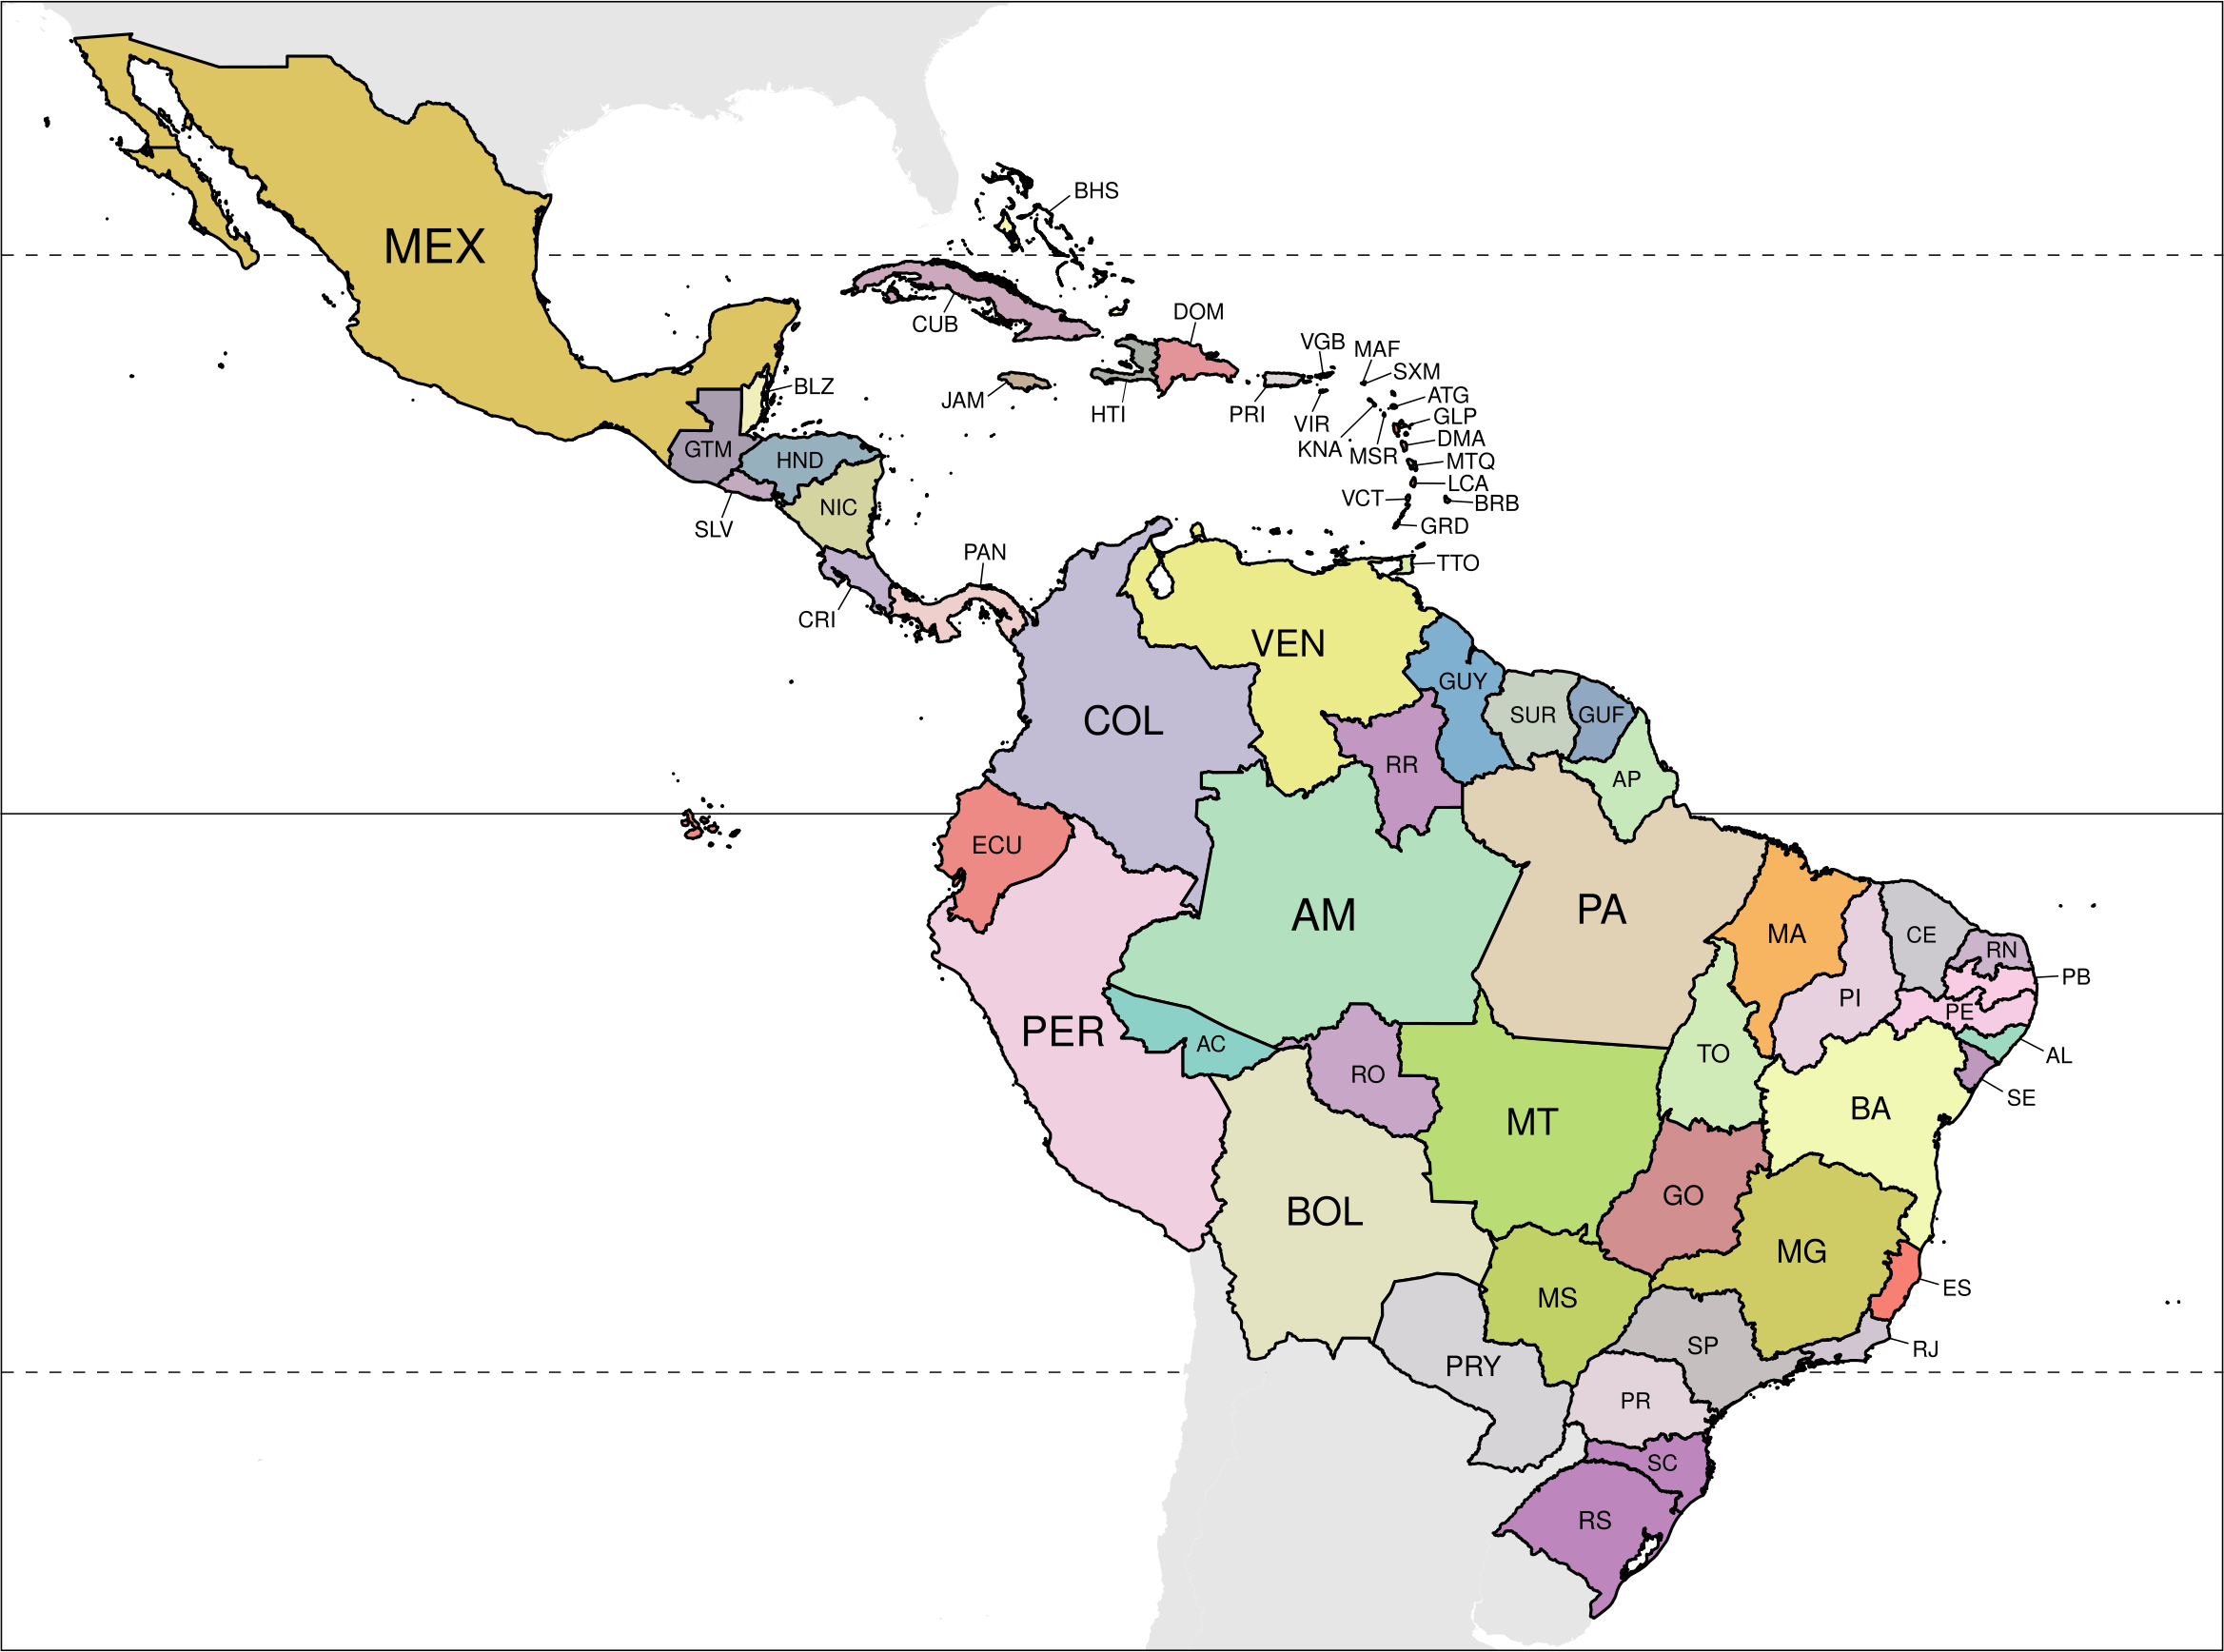
\includegraphics[width=\textwidth]{figs_sm/study_areas_America} \end{center}

\begin{center}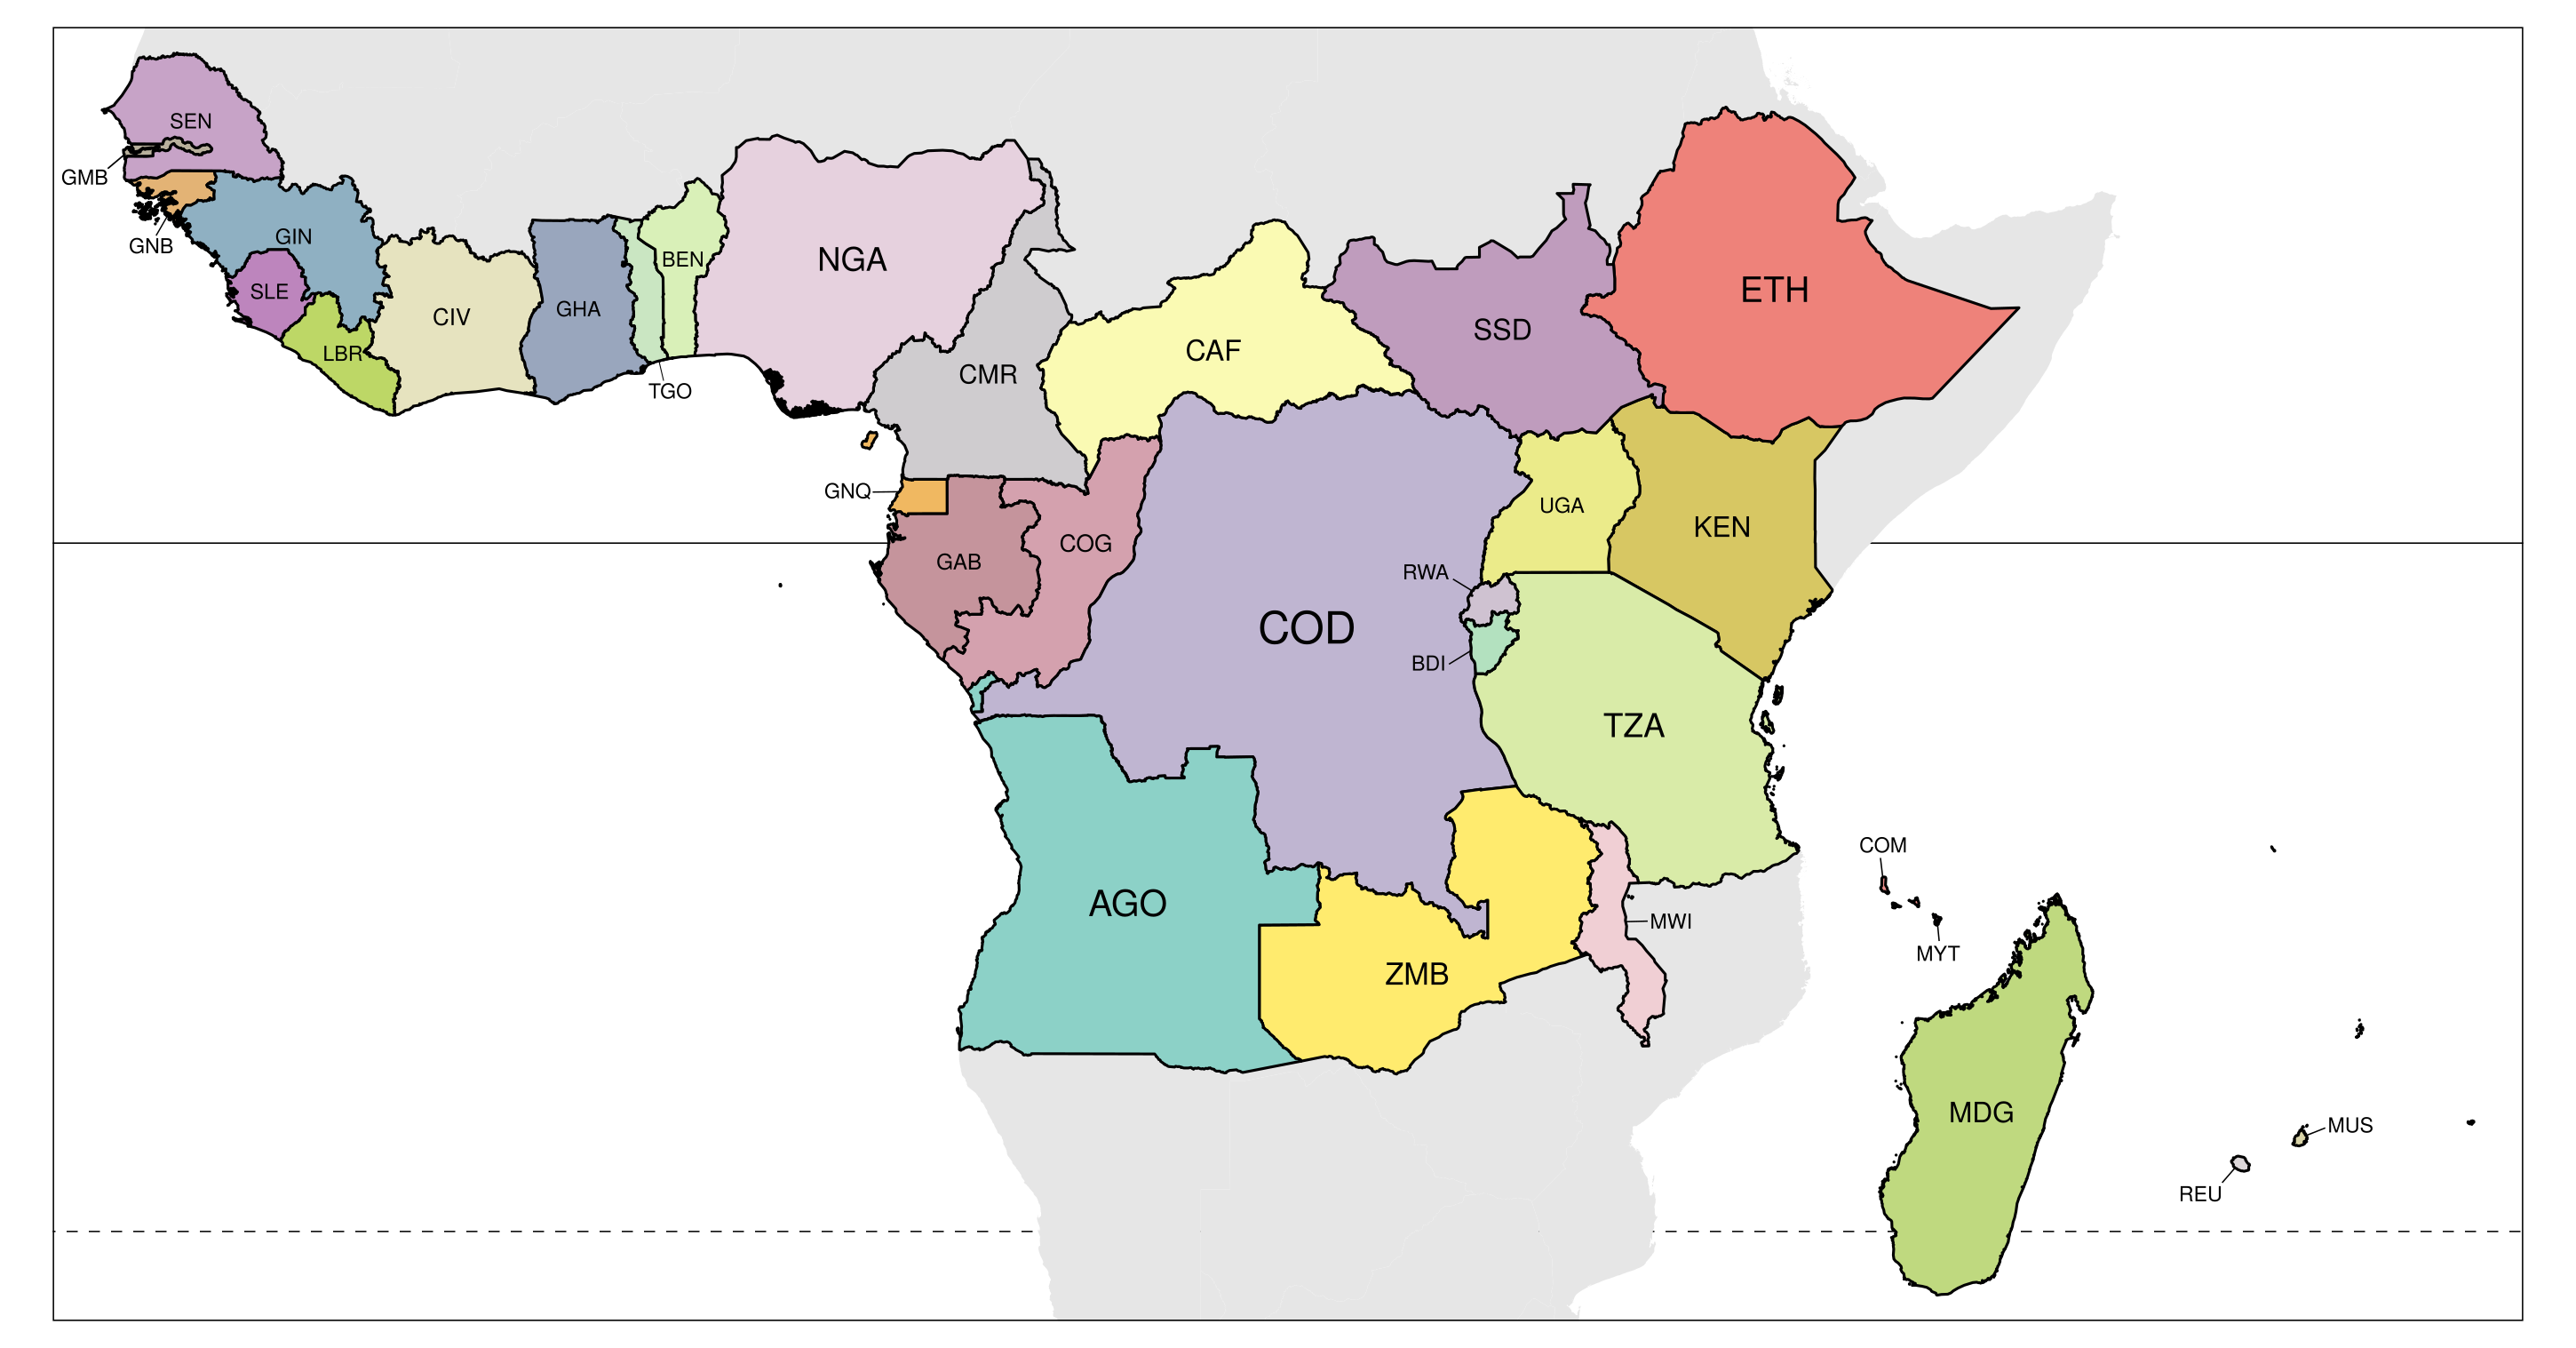
\includegraphics[width=\textwidth]{figs_sm/study_areas_Africa} \end{center}

\begin{figure}[H]

{\centering 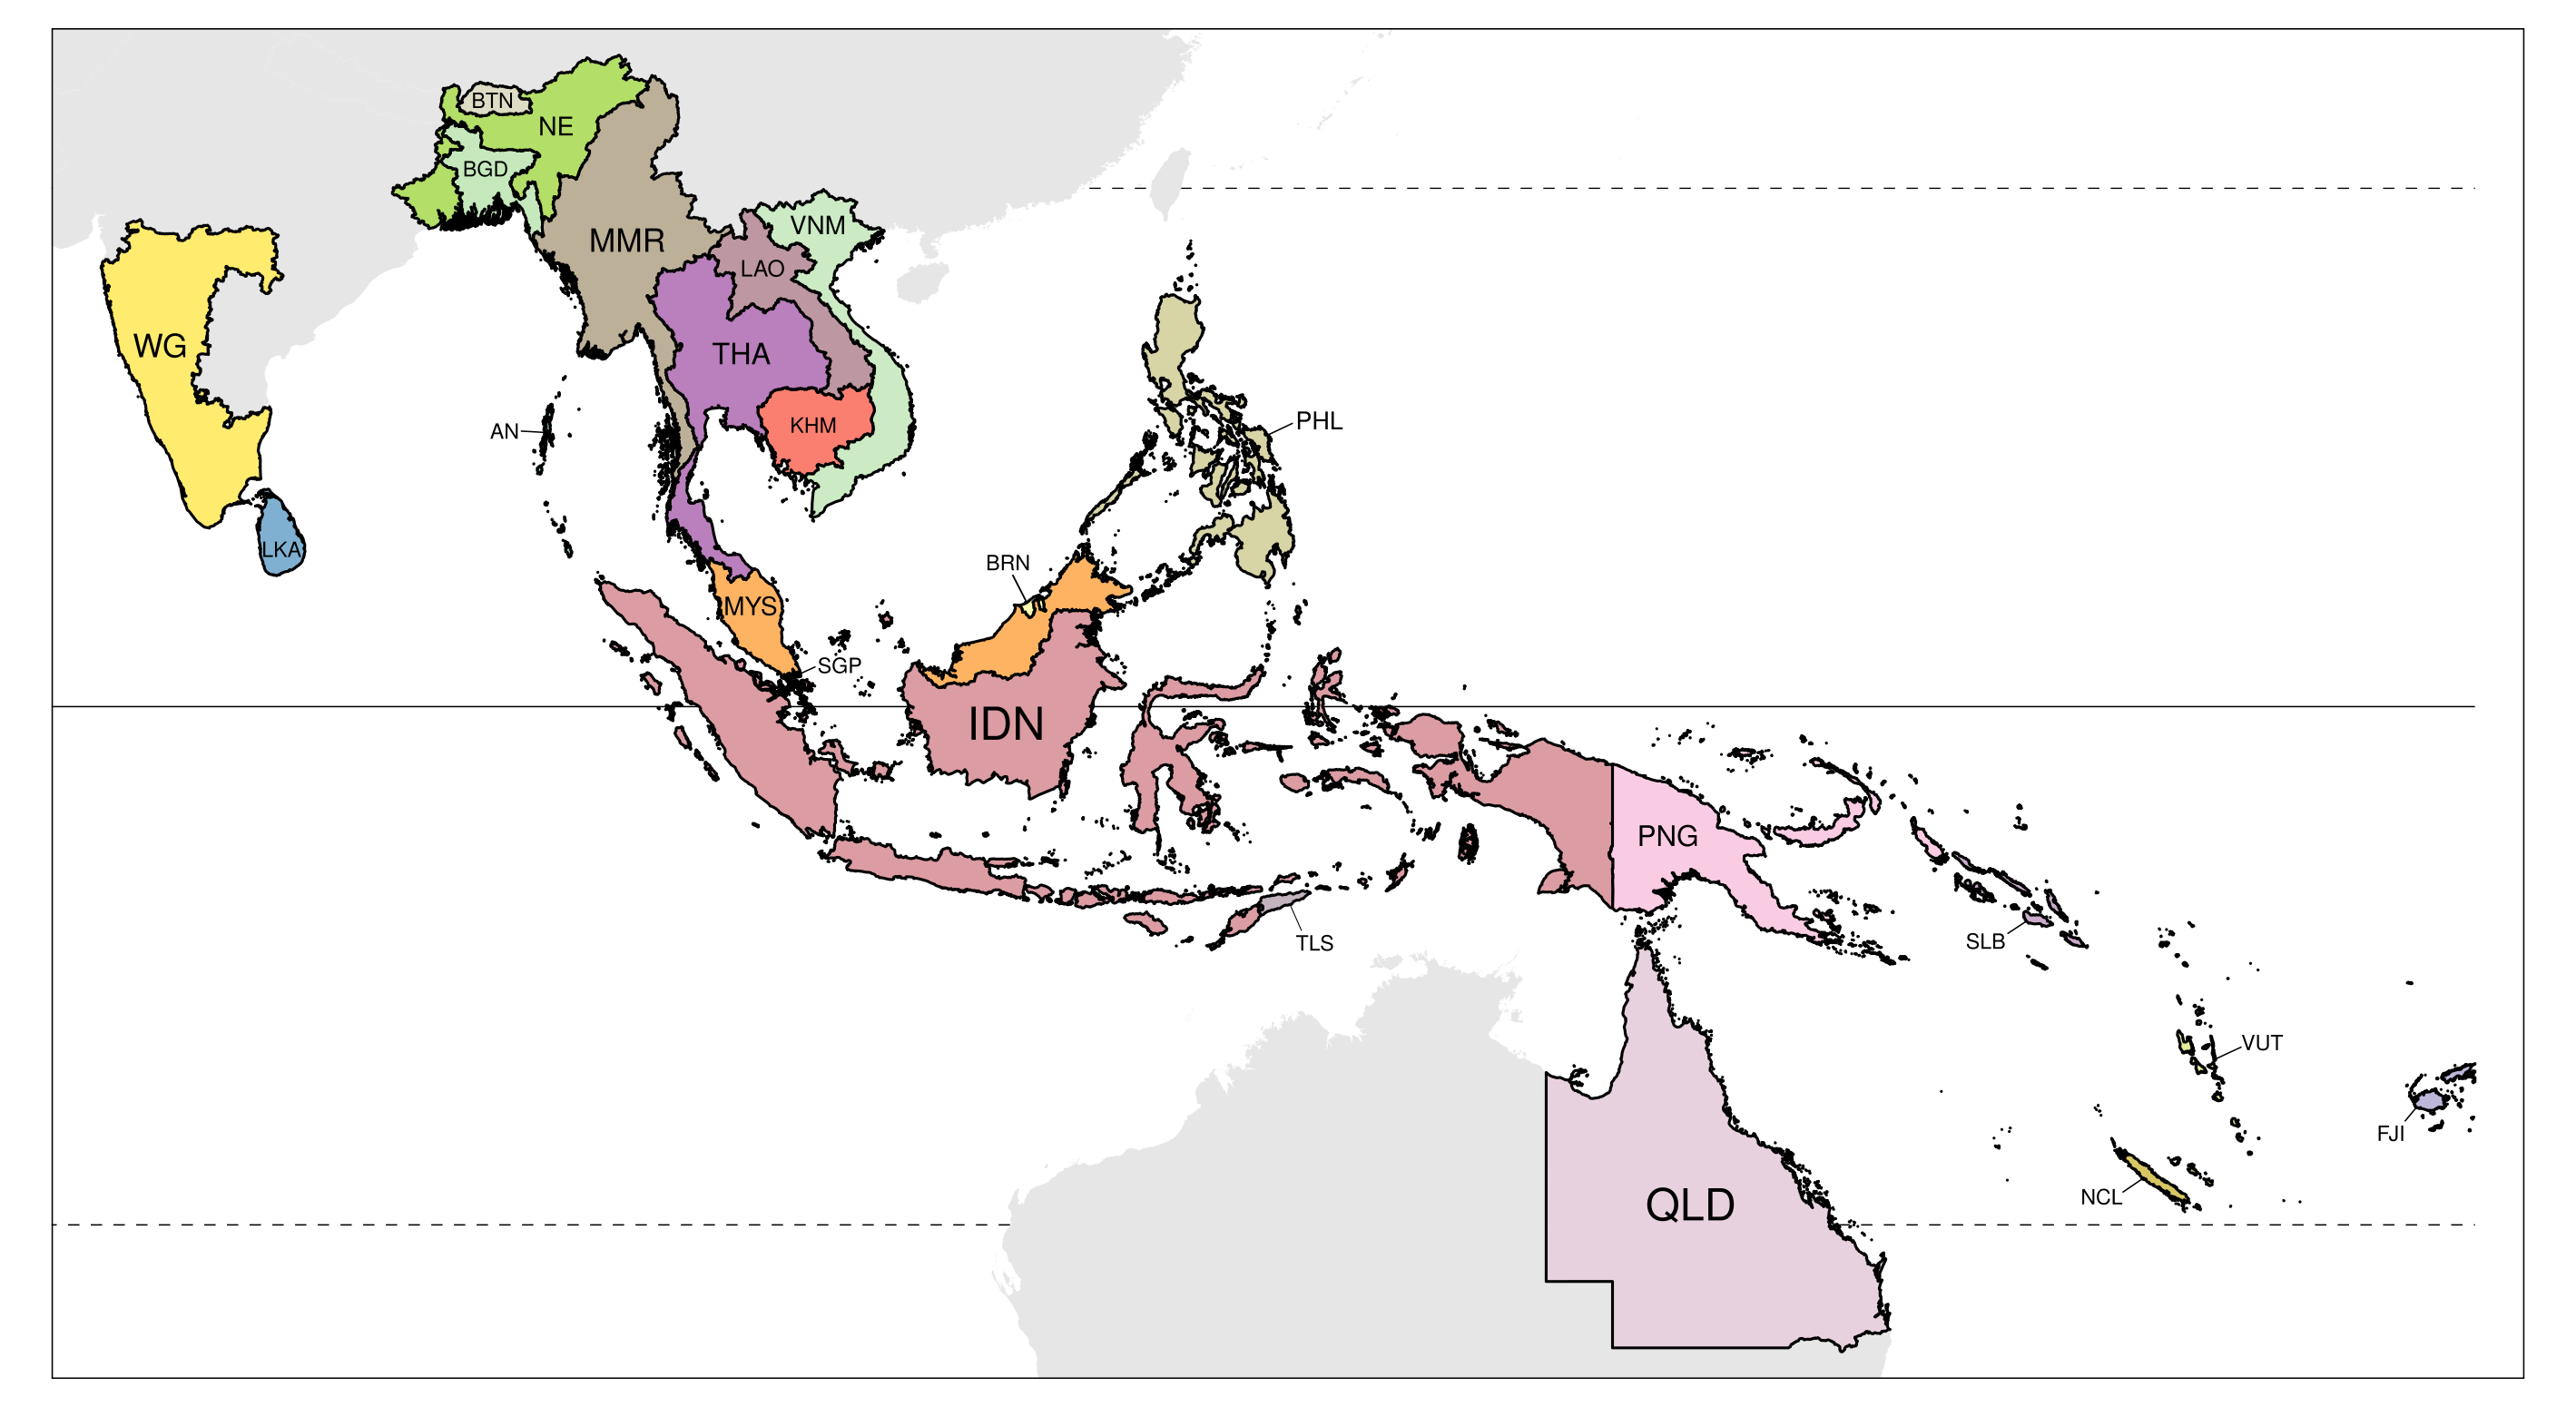
\includegraphics[width=\textwidth]{figs_sm/study_areas_Asia} 

}

\caption{\textbf{Study areas in the three continents: America, Africa, and Asia}. America included 64 study areas (39 countries), Africa included 32 study areas (32 countries), and Asia included 23 study areas (21 countries). Each country was identified by one unique three-letter code following the ISO 3166-1 standard (eg. MDG for Madagascar or GUF for French Guiana). In America, Brazil was divided in 26 study areas corresponding to the 26 Brazilian states. Each Brazilian state was defined by one unique two-letter code (eg. AM for Amazonas). For India, three study areas were considered: the Whestern Ghats (WG), the North-East India (NE), and the Andaman and Nicobar Islands (AN). For Australia, we only considered the Queensland (QLD) state as a study area. In the three figures, each study area is identified by one unique code and a set of polygons with the same colour. The horizontal lines on each figure indicate the position of the Equator (plain line) and the two tropics (Cancer at the North and Capricorn at the South, dashed lines).}\label{fig:study-areas}
\end{figure}

\hypertarget{past-forest-cover-change-map}{%
\subsection{Past forest cover change map}\label{past-forest-cover-change-map}}



\begin{figure}[H]

{\centering 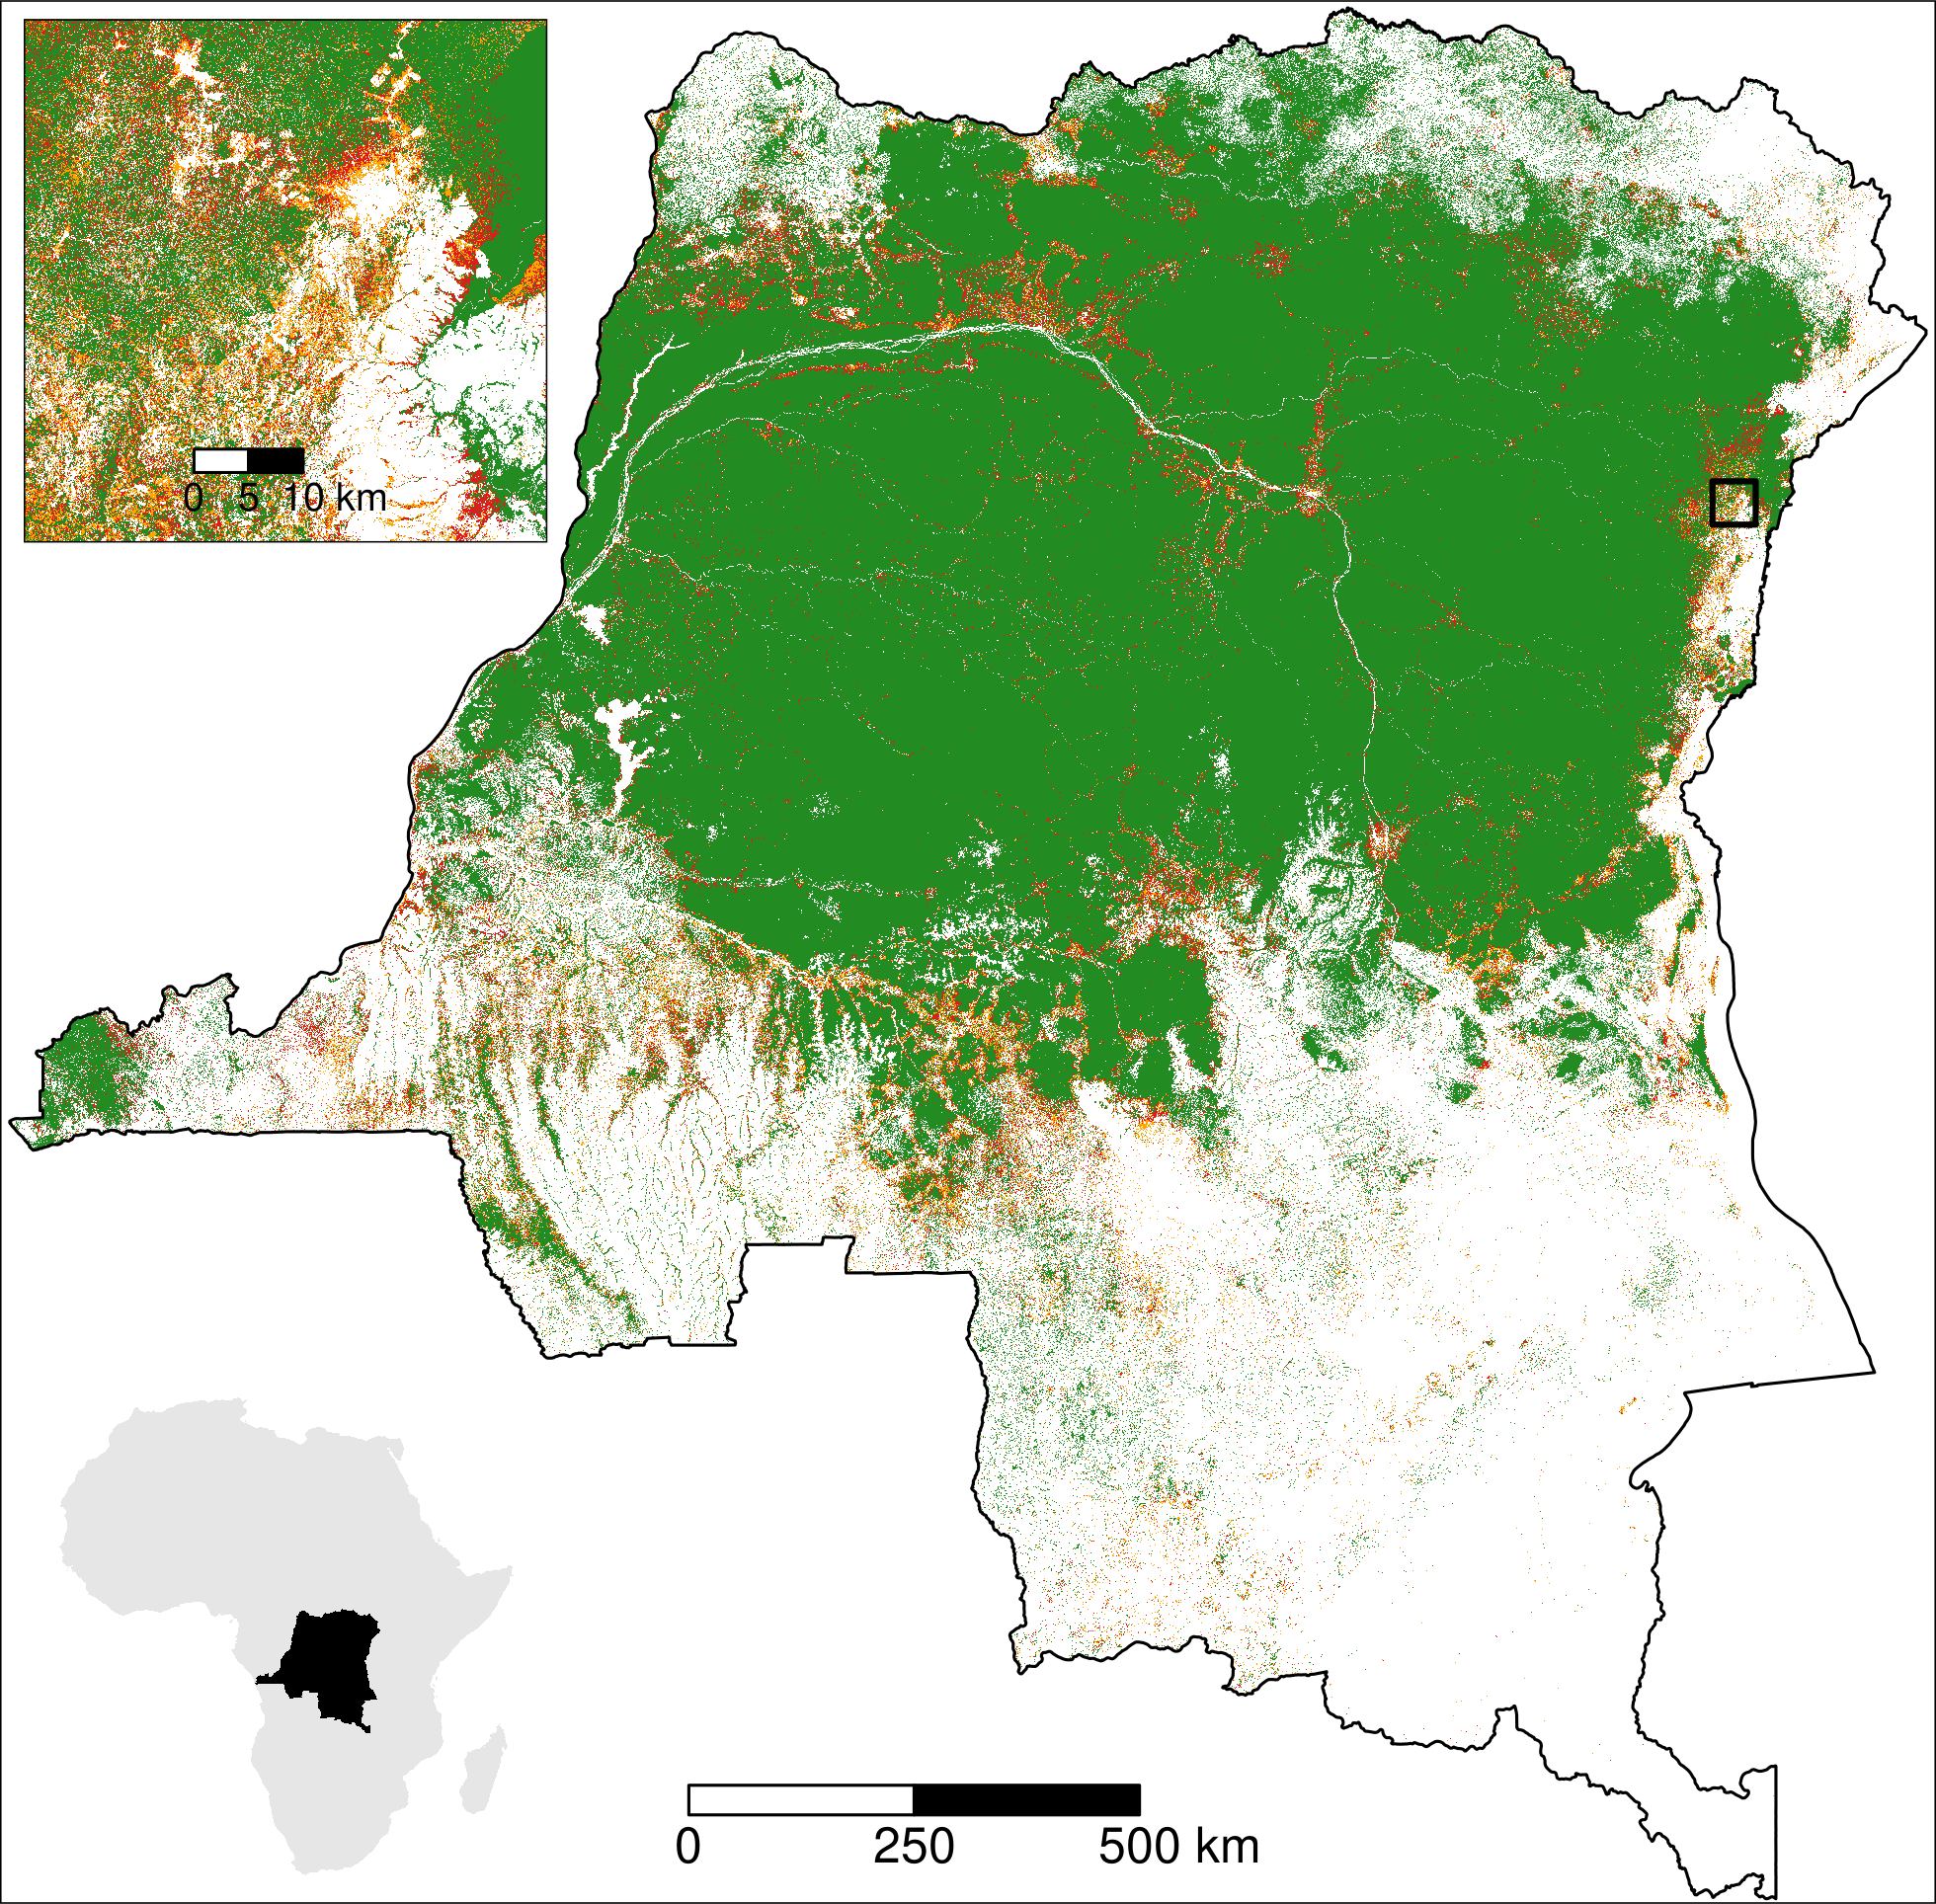
\includegraphics[width=\textwidth]{figs_sm/fcc123} 

}

\caption{\textbf{Past forest cover change map}. Forest cover change map on the period 2000--2010--2020 for the Democratic Republic of the Congo in central Africa (bottom-left inset). \textcolor{orange}{orange}: 2000--2010 deforestation, \textcolor{red}{red}: 2010--2020 deforestation, \textcolor{darkgreen}{green}: forest cover in 2020. Forest cover change map was derived from the forest cover change annual product by Vancutsem \emph{et al.} \citep{Vancutsem2021}. Original resolution of the forest cover change map is 30 m. The top-left inset shows a zoom of the map for an area at the North-East of the country which is close to the city of Beni and the Virunga national park. An interactive pantropical forest cover change map is available at \url{https://forestatrisk.cirad.fr/maps.html}.}\label{fig:fcc-maps}
\end{figure}

\hypertarget{spatial-explanatory-variables-used-for-spatial-modelling-of-deforestation}{%
\subsection{Spatial explanatory variables used for spatial modelling of deforestation}\label{spatial-explanatory-variables-used-for-spatial-modelling-of-deforestation}}



\begin{figure}[H]

{\centering 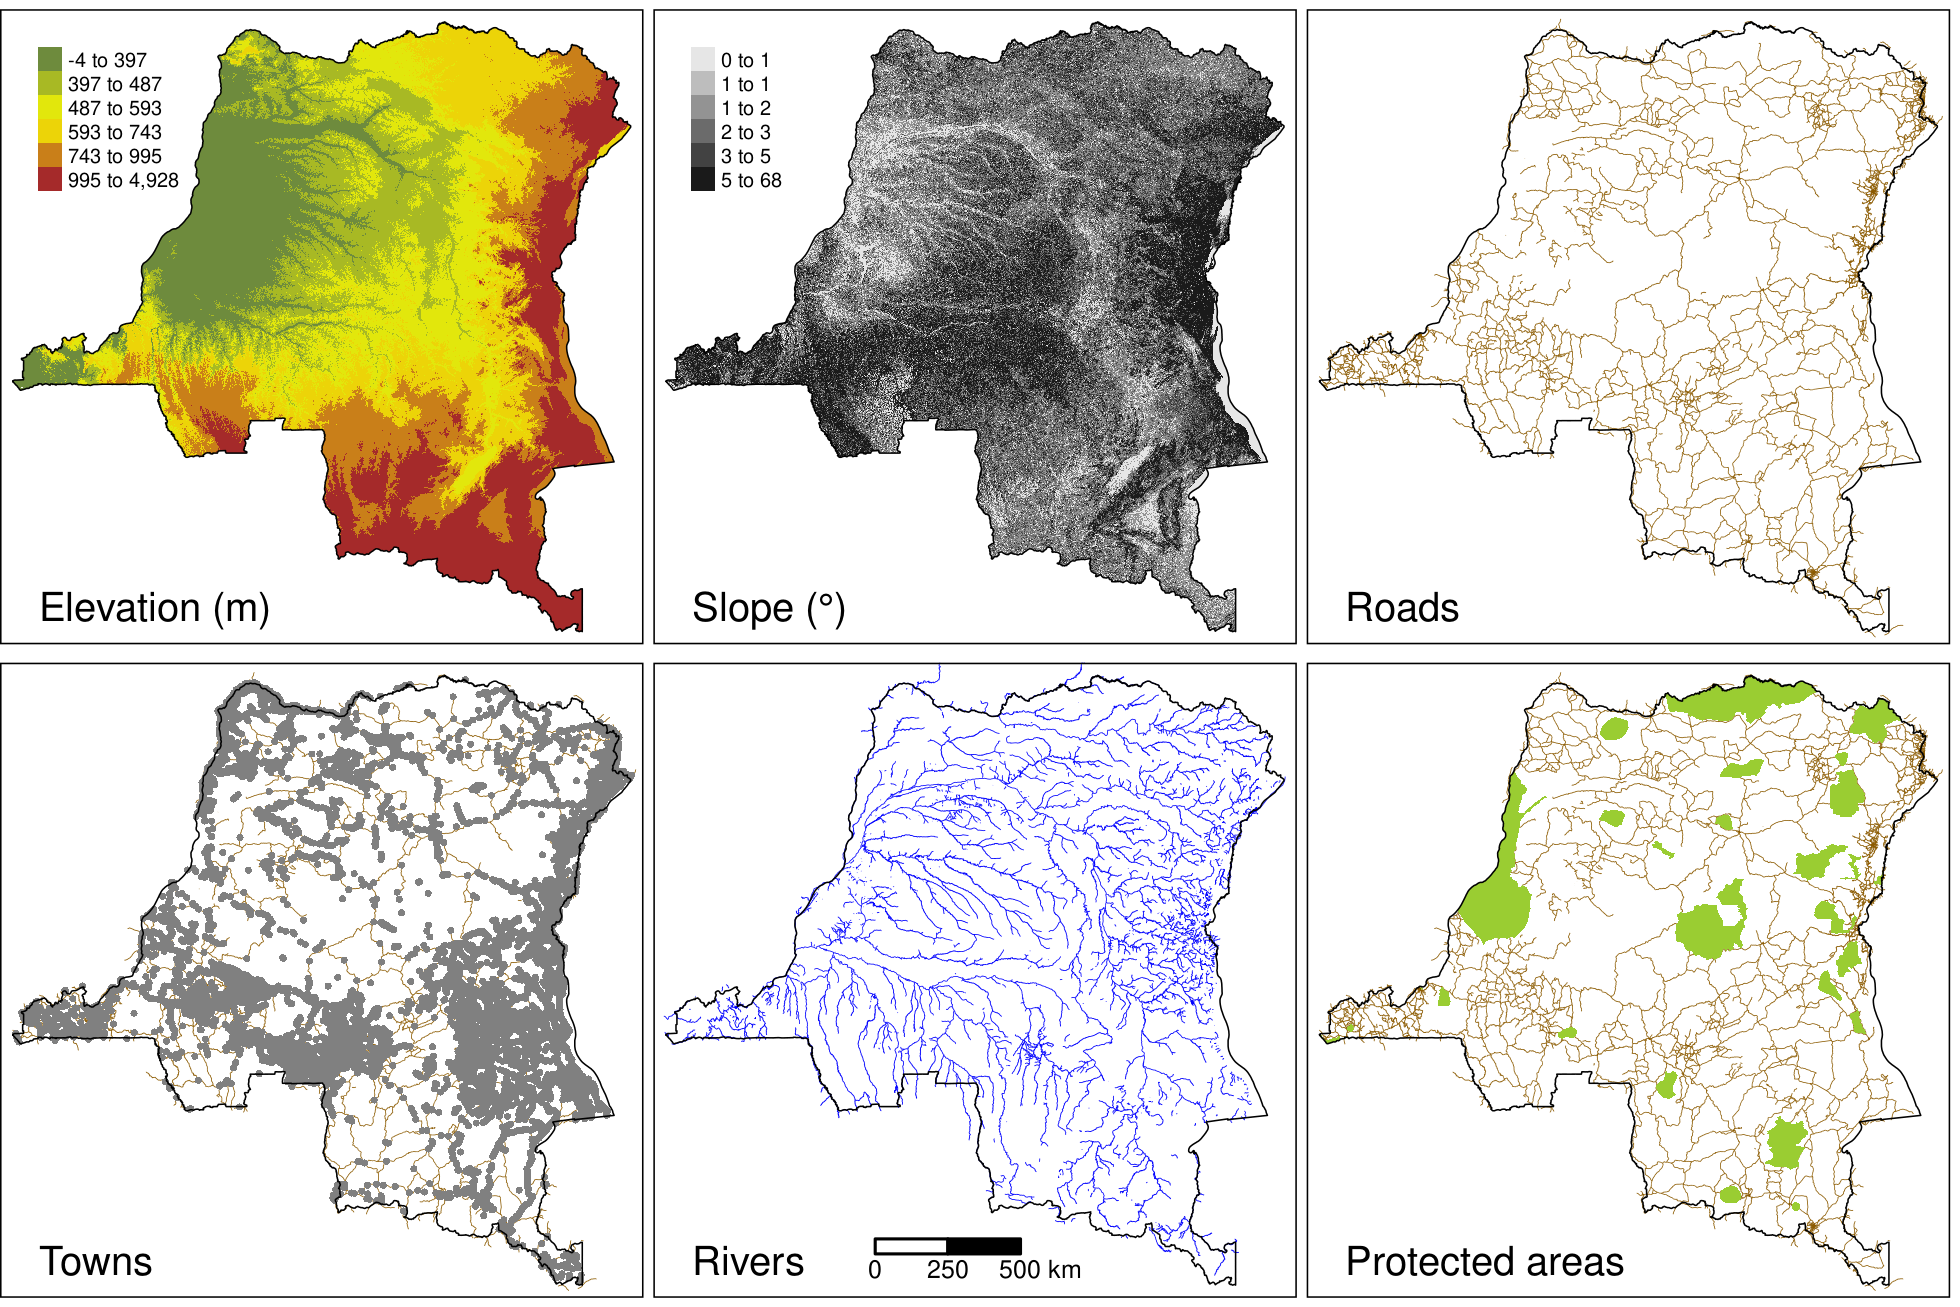
\includegraphics[width=\textwidth]{figs_sm/var} 

}

\caption{\textbf{Spatial explanatory variables}. Spatial explanatory variables for the Democratic Republic of the Congo in central Africa. Elevation (in m) and slope (in degree) at 90 m resolution were obtained from the SRTM Digital Elevation Database v4.1 (\url{http://srtm.csi.cgiar.org/}). Distances (in m) to nearest road, town and river at 150 m resolution were computed from the road, town and river network obtained from OpenStreetMap (OSM) (\url{https://www.openstreetmap.org/}). Roads include ``motorway'', ``trunk'', ``primary'', ``secondary'' and ``tertiary'' roads from OSM. Towns include ``city'', ``town'' and ``village'' categories from OSM. Rivers include ``river'' and ``canal'' categories from OSM. Protected areas were obtained from the World Database on Protected Areas (\url{https://www.protectedplanet.net} \citep{WDPA2020}). We retained protected areas defined by at least one polygon and which had the following status: ``Designated'', ``Inscribed'', ``Established'', or ``Proposed'' before 1\textsuperscript{st} January 2010. Data included protected areas of all IUCN categories (from Ia to VI) and of all types defined at the national level (e.g.~National Parks, Reserves). Two additional spatial explanatory variables (distance to forest edge and distance to past deforestation) were obtained from the past forest cover change map (Fig.~\ref{fig:fcc-maps}).}\label{fig:var}
\end{figure}



\begin{figure}[H]

{\centering 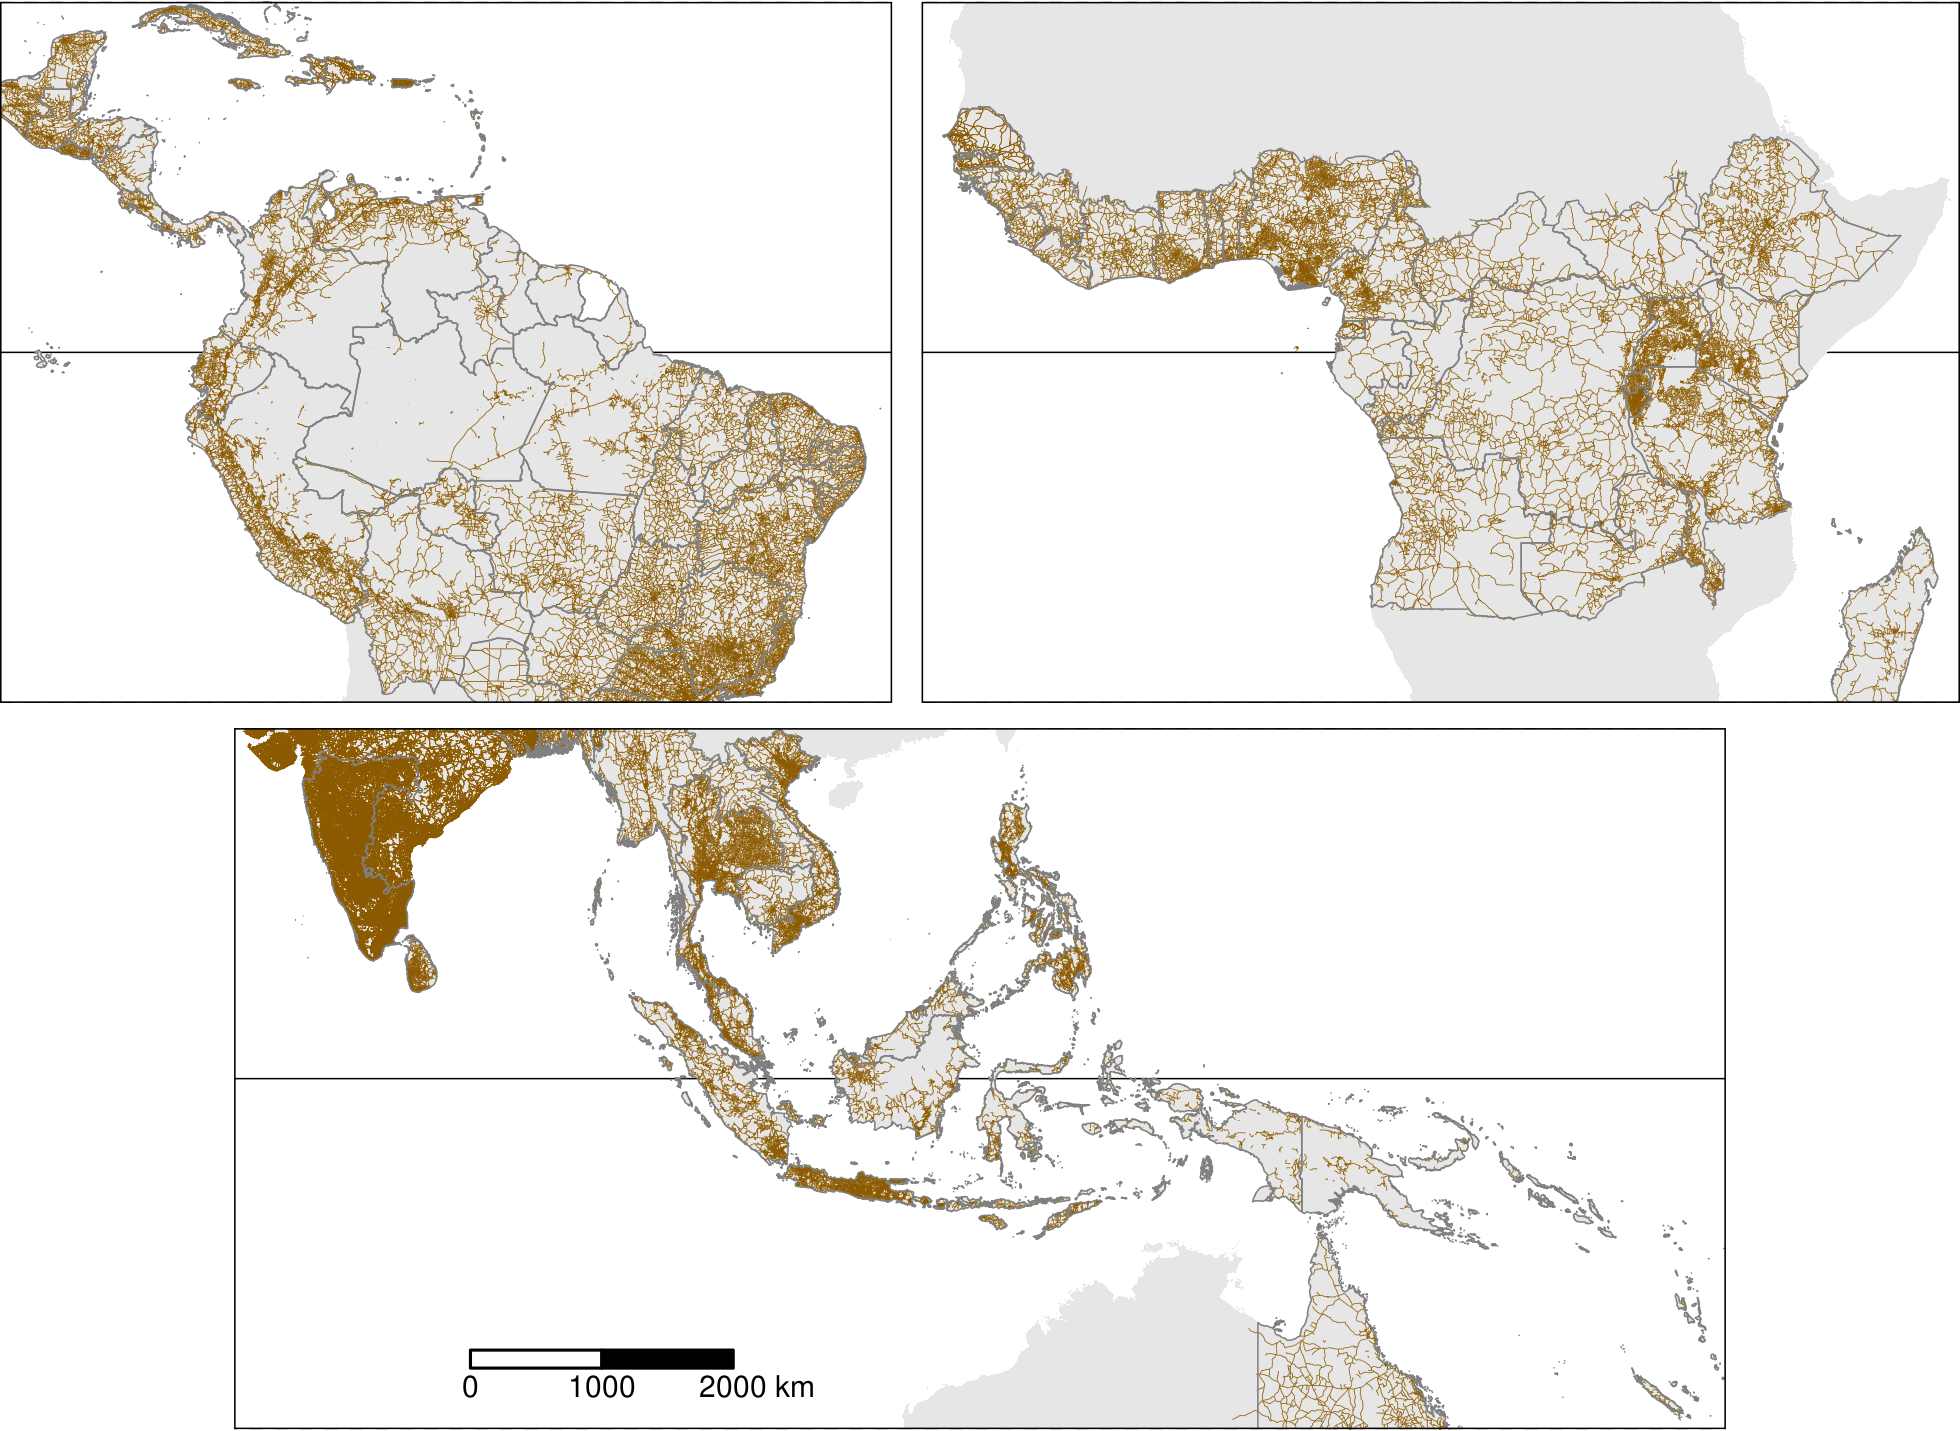
\includegraphics[width=\textwidth]{figs_sm/roads} 

}

\caption{\textbf{Pantropical road network}. The road network was obtained from OpenStreetMap (OSM) (\url{https://www.openstreetmap.org/}). Roads included ``motorway'', ``trunk'', ``primary'', ``secondary'' and ``tertiary'' roads from OSM. Our dataset included a total of 3,606,841 roads.}\label{fig:data-roads}
\end{figure}



\begin{figure}[H]

{\centering 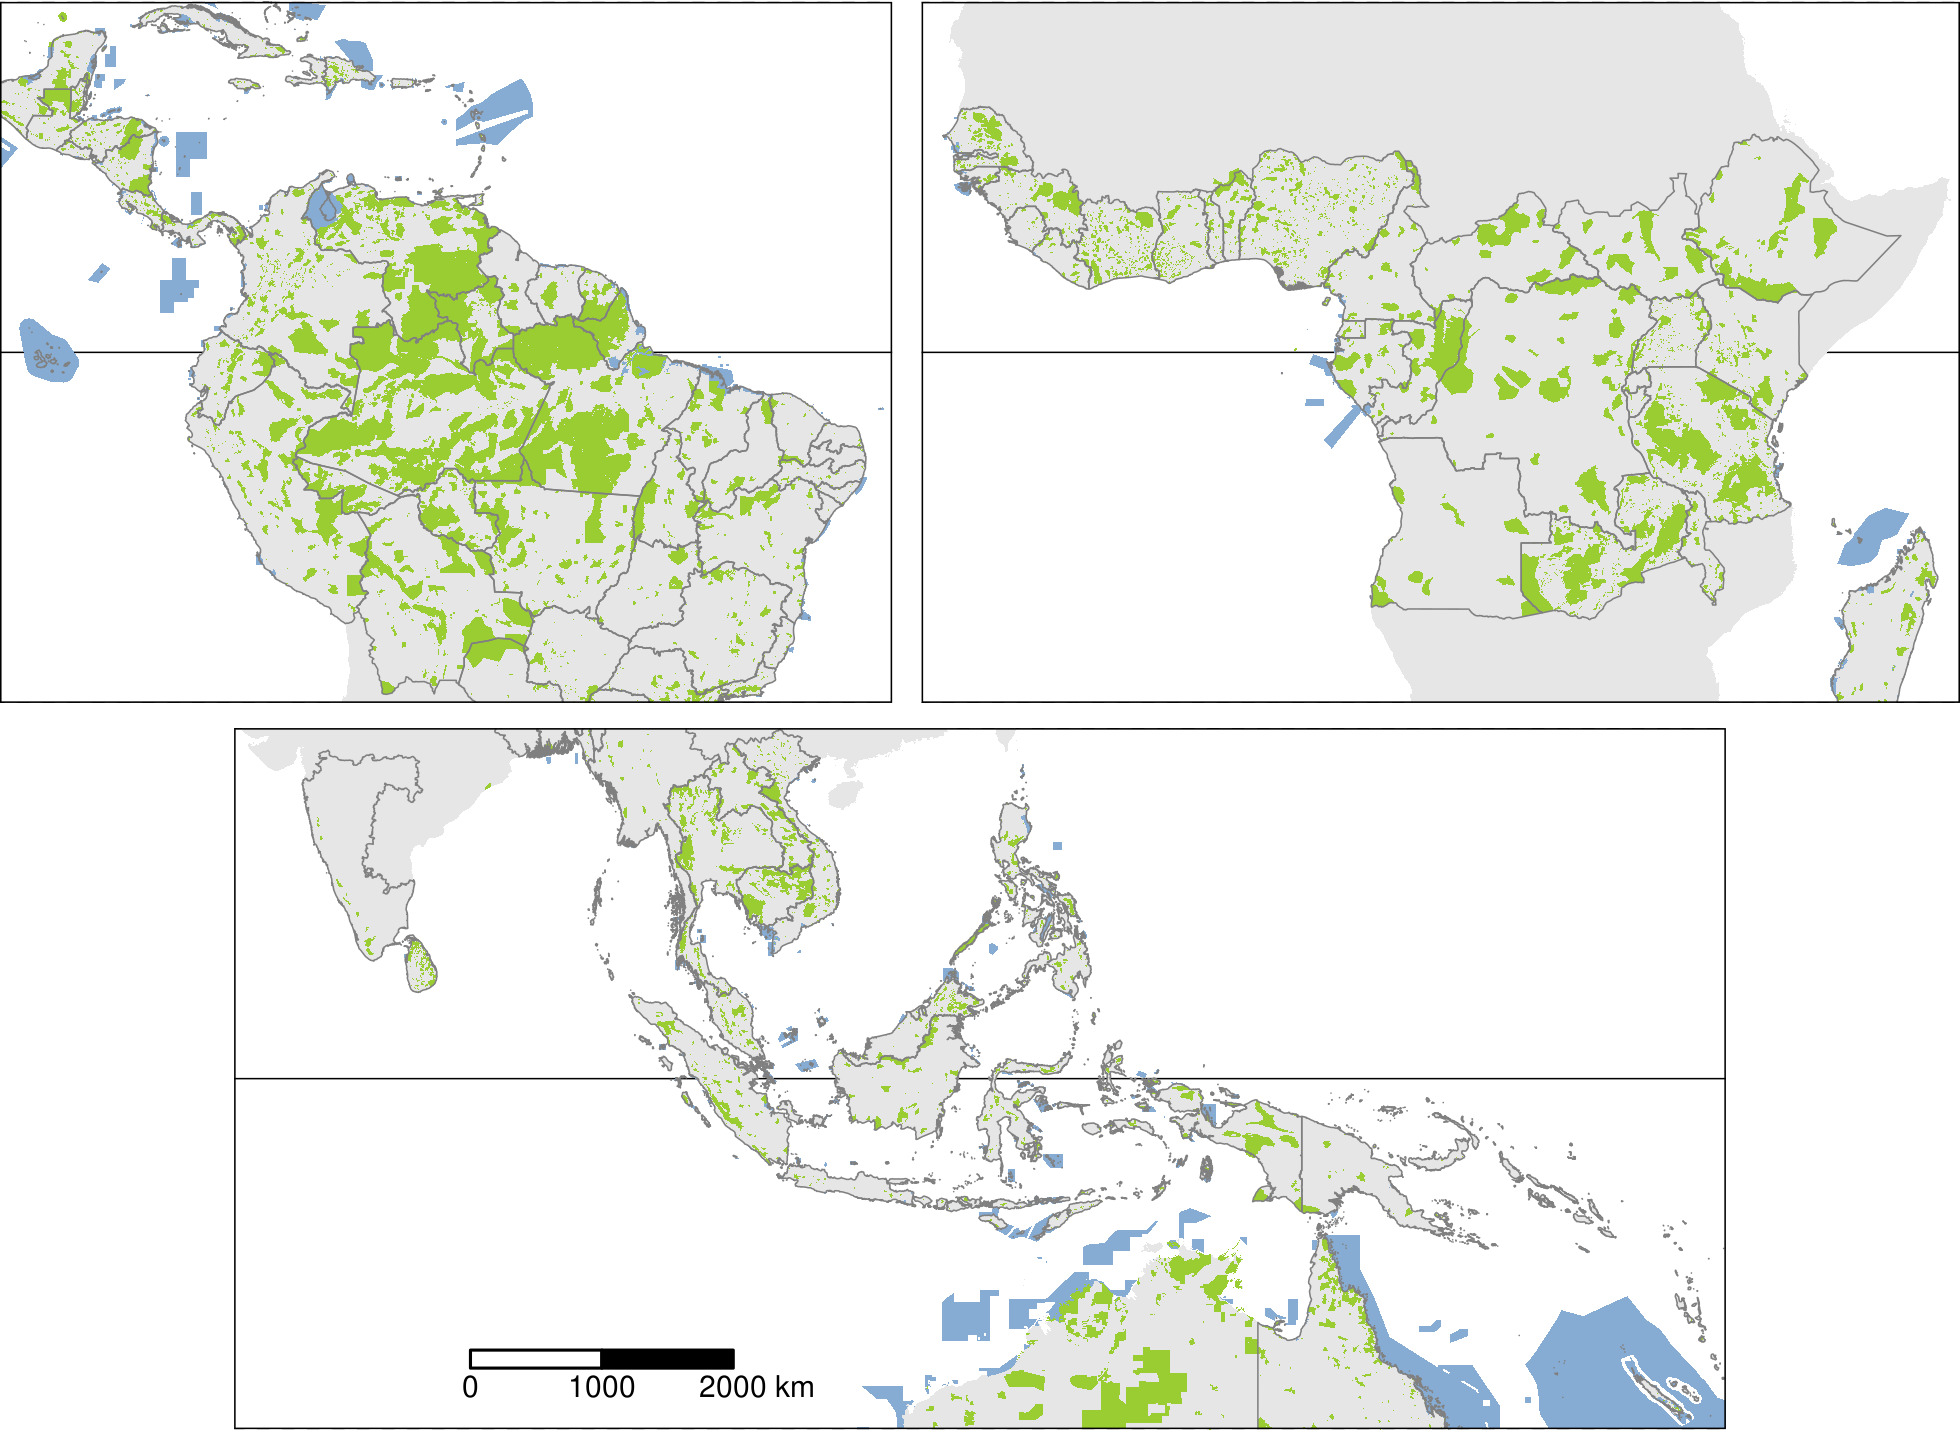
\includegraphics[width=\textwidth]{figs_sm/pa} 

}

\caption{\textbf{Pantropical data-set on protected areas}. Terrestrial protected areas in \textcolor[HTML]{5c7b1e}{green}, marine protected areas in \textcolor[HTML]{51677e}{blue}. Protected areas were downloaded from the World Database on Protected Areas (\url{https://www.protectedplanet.net} \citep{WDPA2020}) using the \texttt{pywdpa} Python package. We retained protected areas defined by at least one polygon and which had the following status: ``Designated'', ``Inscribed'', ``Established'', or ``Proposed'' before 1\textsuperscript{st} January 2010. Data included protected areas of all IUCN categories (from Ia to VI) and of all types defined at the national level (e.g.~National Parks, Reserves). Our dataset included a total of 89,855 protected areas.}\label{fig:data-pa}
\end{figure}



\begin{figure}[H]

{\centering 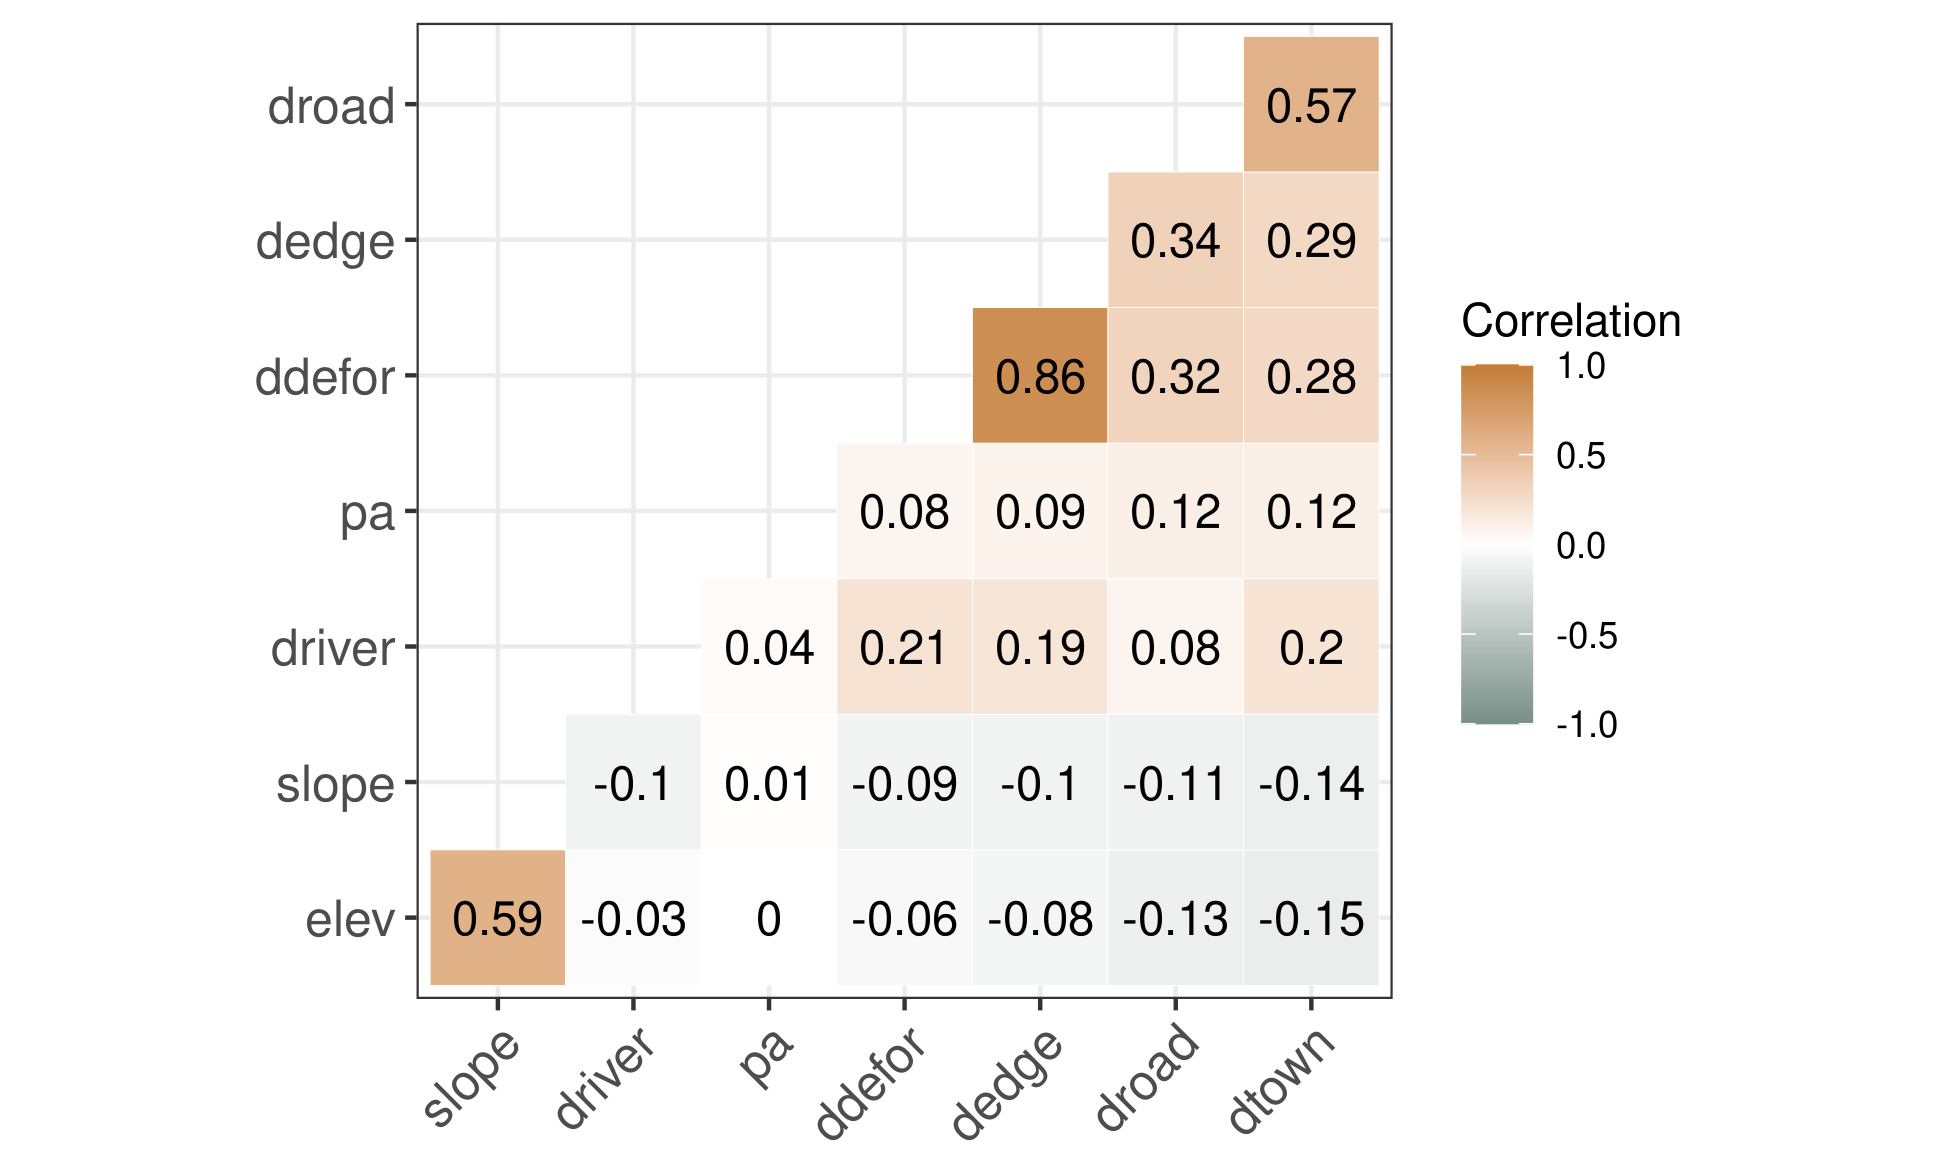
\includegraphics[width=\textwidth]{figs_sm/corr-var} 

}

\caption{\textbf{Correlation between explanatory variables}. To compute the correlations, we used a representative data-set at the global scale where the number of observations for each study area was proportional to its forest cover in 2010. We used a total of 813,796 observations. We computed the Pearson's correlation matrix for the seven continuous explanatory variables used to model the deforestation: elevation (``elev''), slope (``slope''), distance to nearest road, town, and river (``droad'', ``dtown'', and ``driver'', respectively), distance to forest edge (``dedge''), and distance to past deforestation (``ddefor''). For the protected areas (``pa''), which is a categorical variable for which a Pearson's correlation coefficient cannot be computed, we reported the slope coefficient of simple logistic regressions where the probability of presence of a protected area was a function of one intercept and one of the continuous variable (which was normalized).}\label{fig:corr-var}
\end{figure}

\hypertarget{data-sampling}{%
\subsection{Data sampling}\label{data-sampling}}



\begin{figure}[H]

{\centering 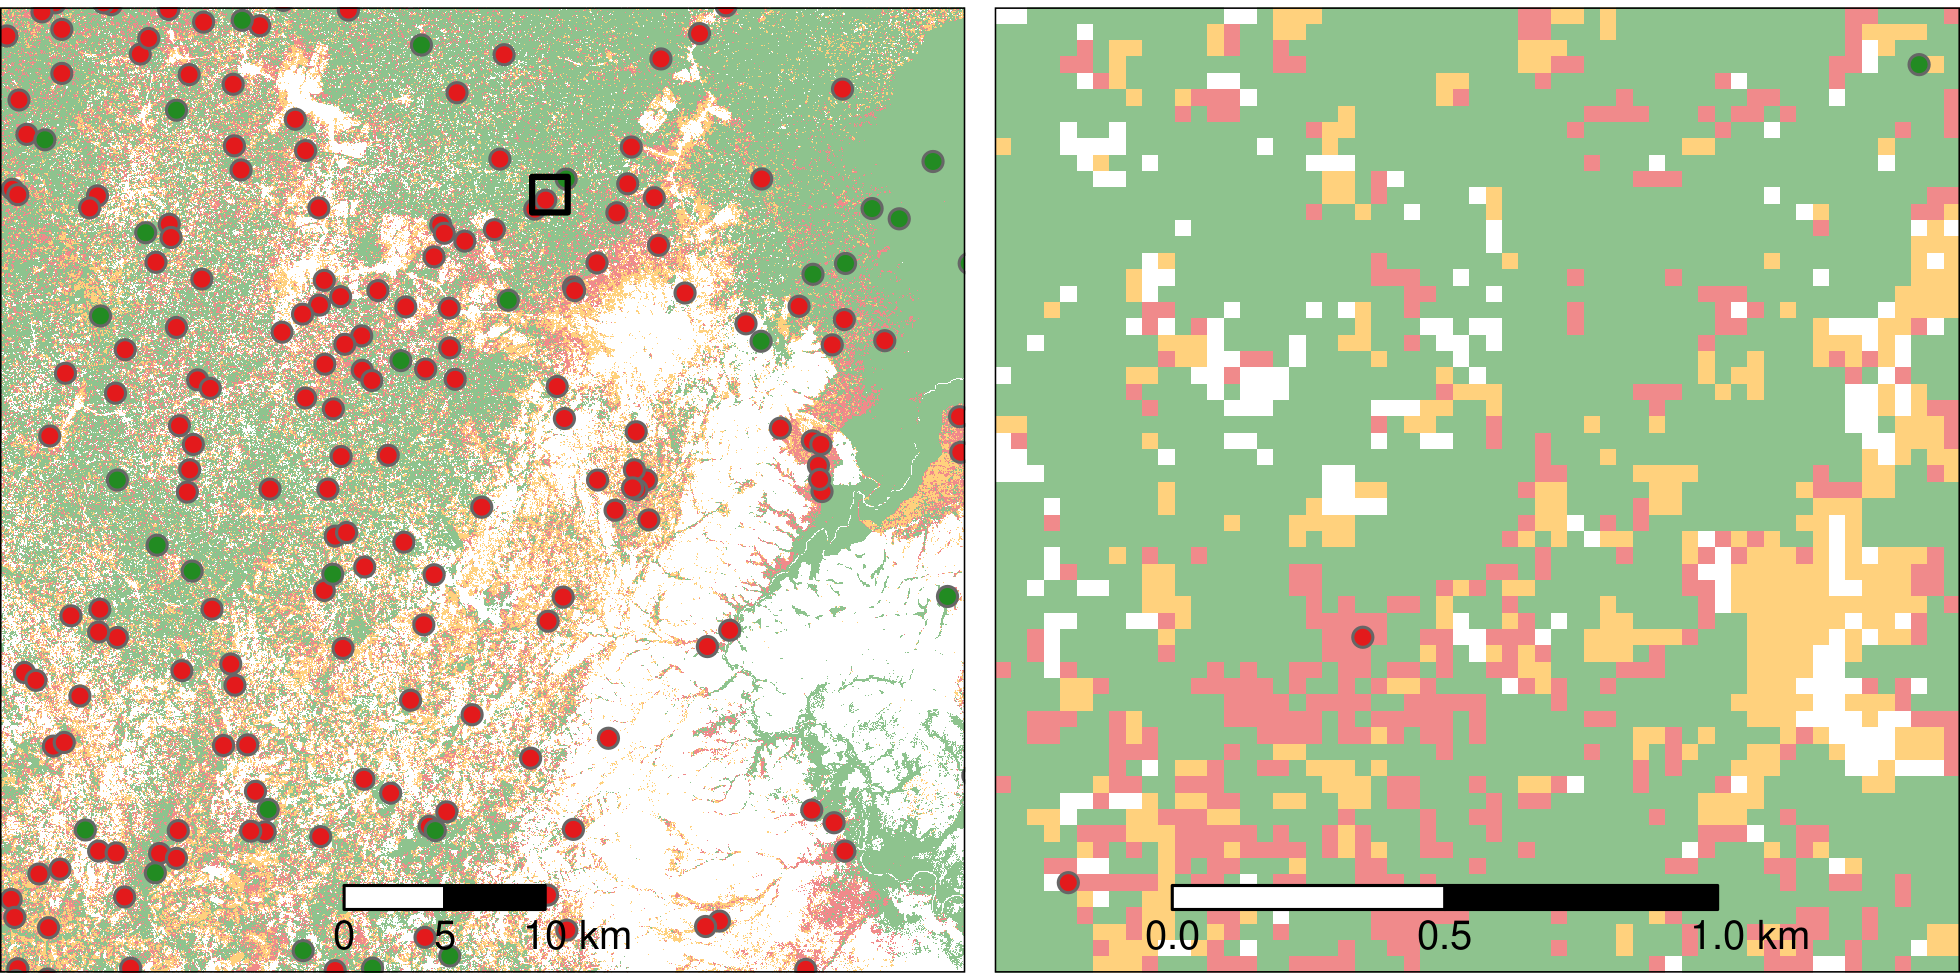
\includegraphics[width=\textwidth]{figs_sm/sample} 

}

\caption{\textbf{Data sampling for spatial modelling of the deforestation}. Map on the left corresponds to the top left inset in Fig.~\ref{fig:fcc-maps} representing a zoom of the forest cover change map on the period 2000--2010--2020 for an area at the North-East of the Democratic Republic of the Congo. Map on the right presents an inner zoom showing the delimitation of the 30 m forest pixels with three sample points. We used a stratified balanced sampling between (i) forest pixels in 2010 which have been deforested on the period 2010--2020 (``deforested'' pixels in \textcolor{red}{red}), and (ii) forest pixels in 2010 which have not been deforested on that period of time and which represent the remaining forest in 2020 (``non-deforested'' pixels in \textcolor{darkgreen}{green}). Forest pixels in each category were sampled randomly.}\label{fig:sampling}
\end{figure}

\hypertarget{grid-for-spatial-random-effects}{%
\subsection{Grid for spatial random effects}\label{grid-for-spatial-random-effects}}



\begin{figure}[H]

{\centering 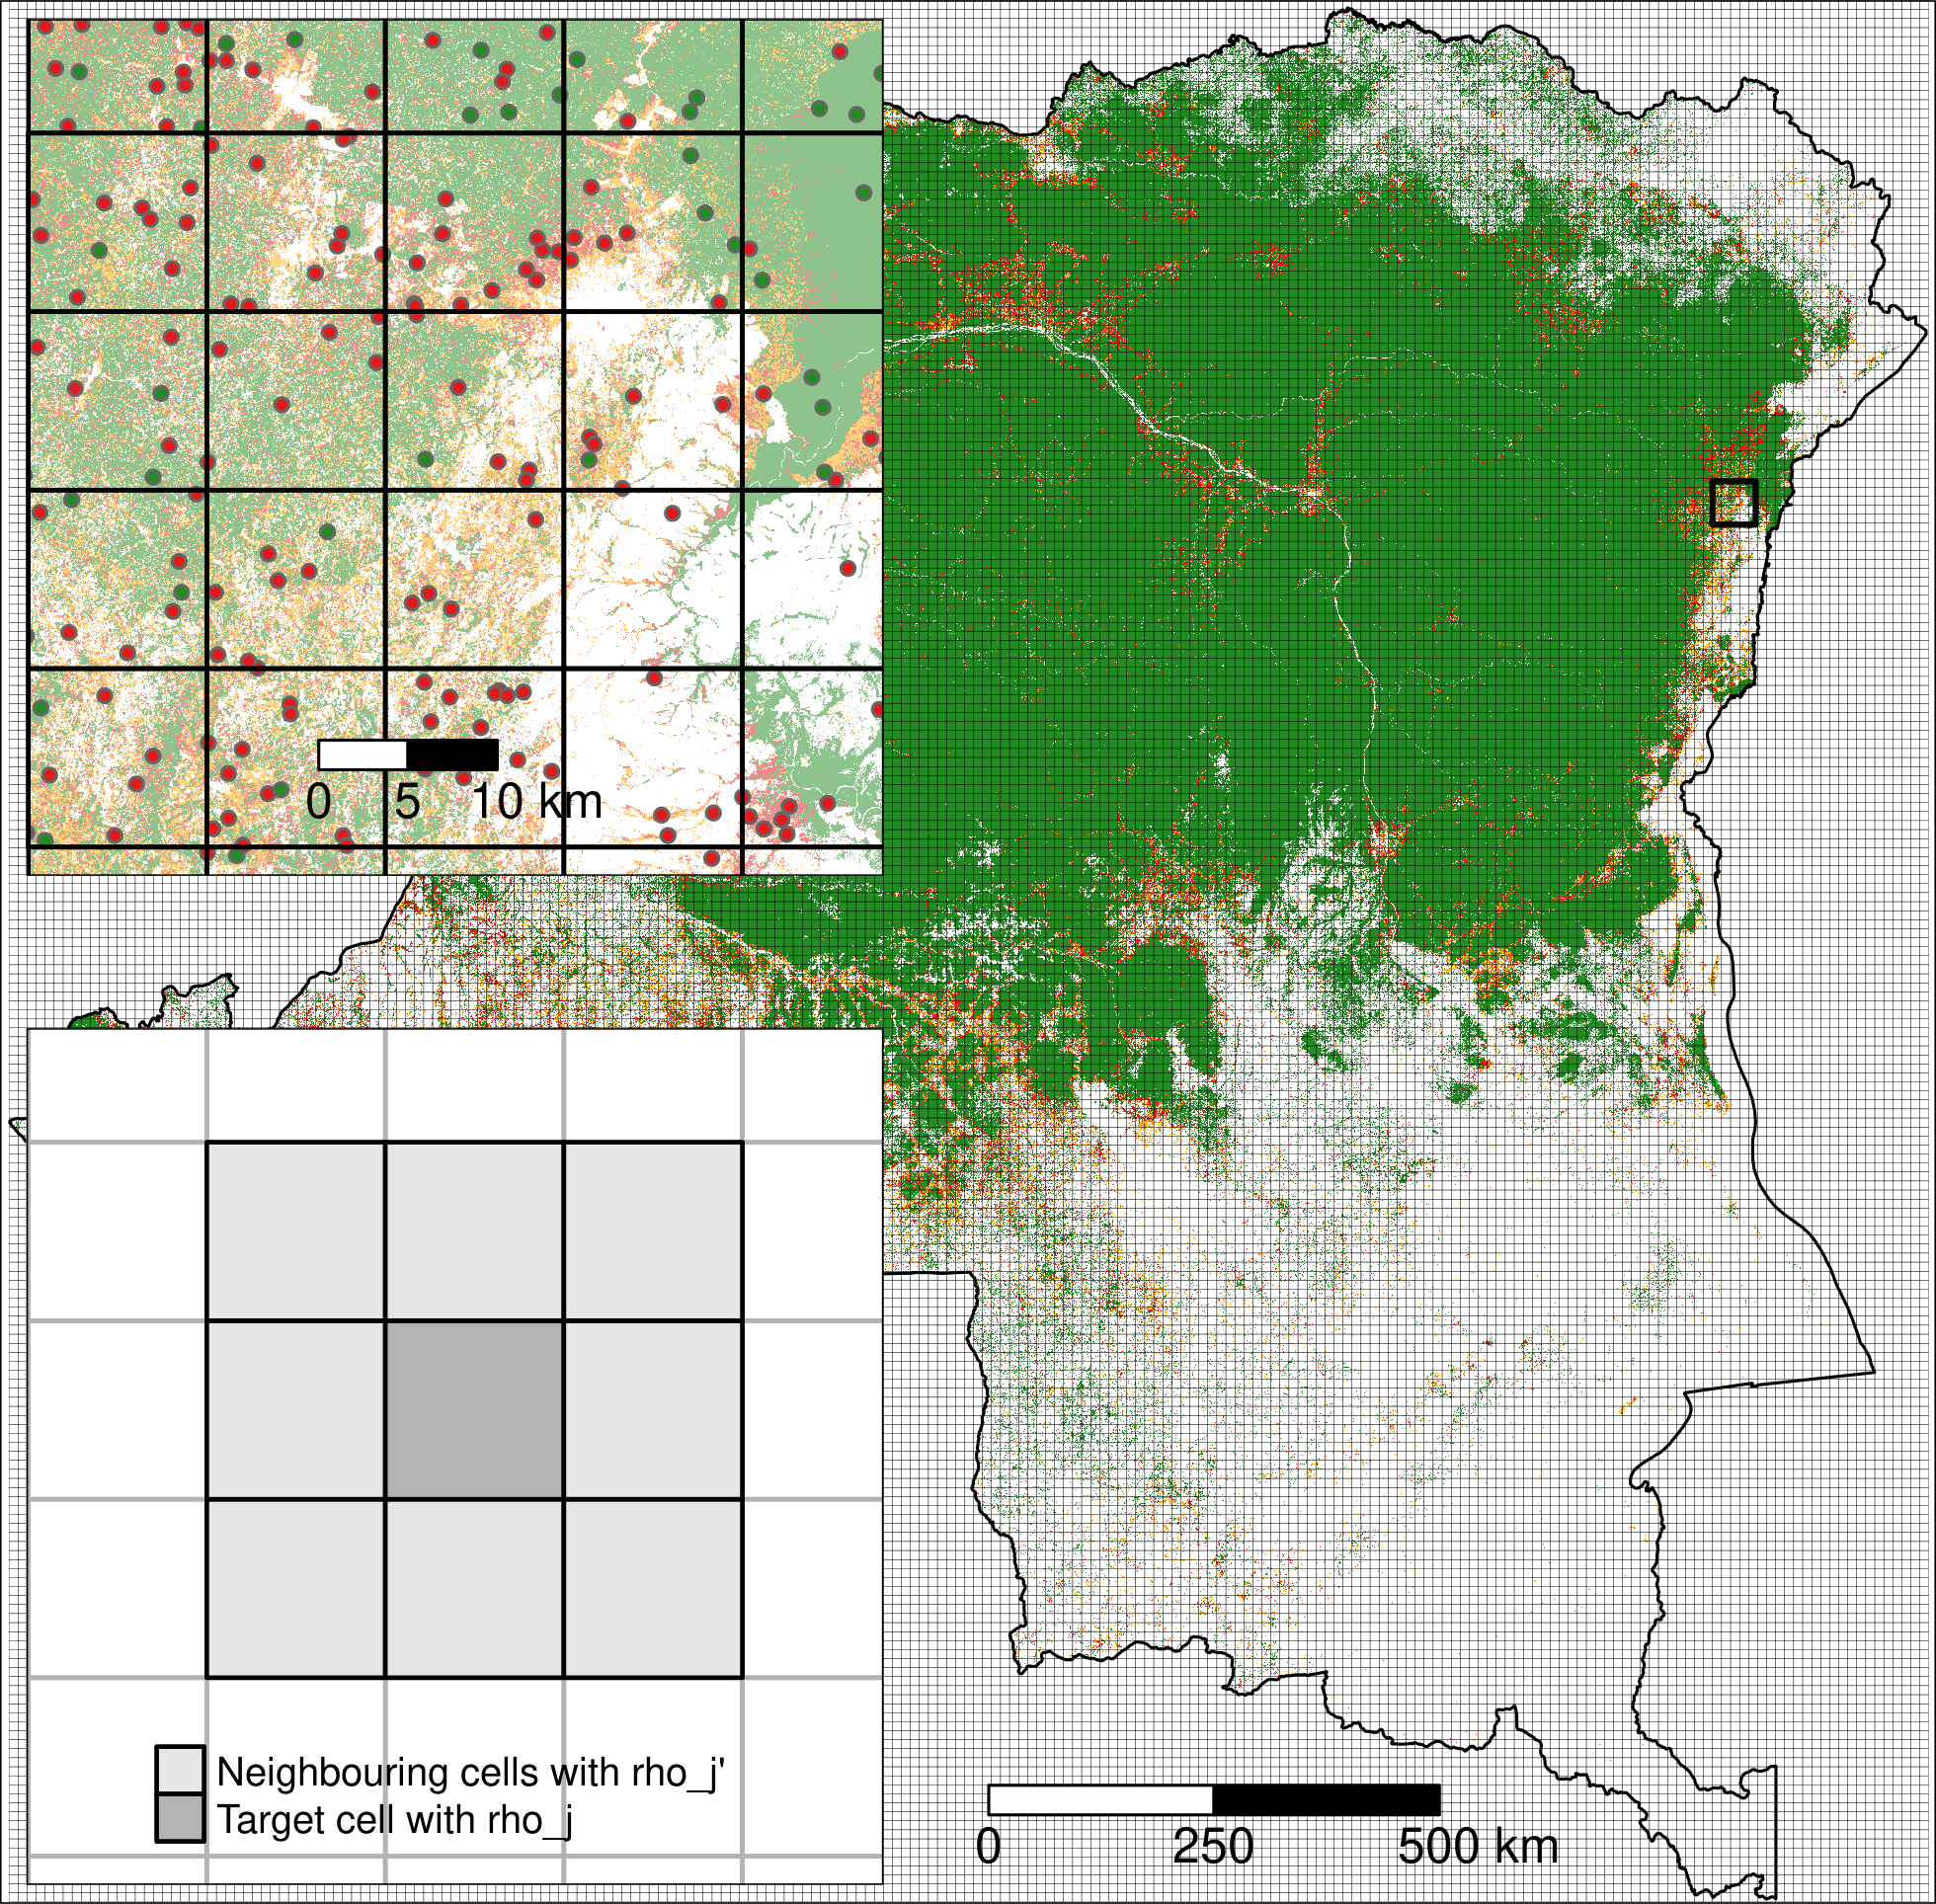
\includegraphics[width=\textwidth]{figs_sm/grid} 

}

\caption{\textbf{Grid used to compute the spatial random effects}. \emph{Main figure}: \(10 \times 10\) km grid covering the Democratic Republic of the Congo (DRC). The grid over DRC includes 45,154 \(10 \times 10\) km cells (214 cells on the x axis by 211 cells on the y axis). The background map shows the past forest cover change in the periods 2000--2010--2020 (see Fig.~\ref{fig:fcc-maps}). \emph{Top inset}: Zoom for an area at the North-East of the country (black square) showing specific grid cells. One grid cell can include several sample points (see Fig.~\ref{fig:sampling}). \emph{Bottom inset}: One random effect \(\rho_j\) is estimated for each grid cell \(j\). Spatial autocorrelation is taken into account through an intrinsic CAR process: the value of the random effect for one cell depends on the values of the random effects \(\rho_{j^{\prime}}\) for the neighbouring cells \(j^{\prime}\) (see Eq.~\eqref{eq:icar}).}\label{fig:grid}
\end{figure}

\hypertarget{estimated-spatial-random-effects}{%
\subsection{Estimated spatial random effects}\label{estimated-spatial-random-effects}}



\begin{figure}[H]

{\centering 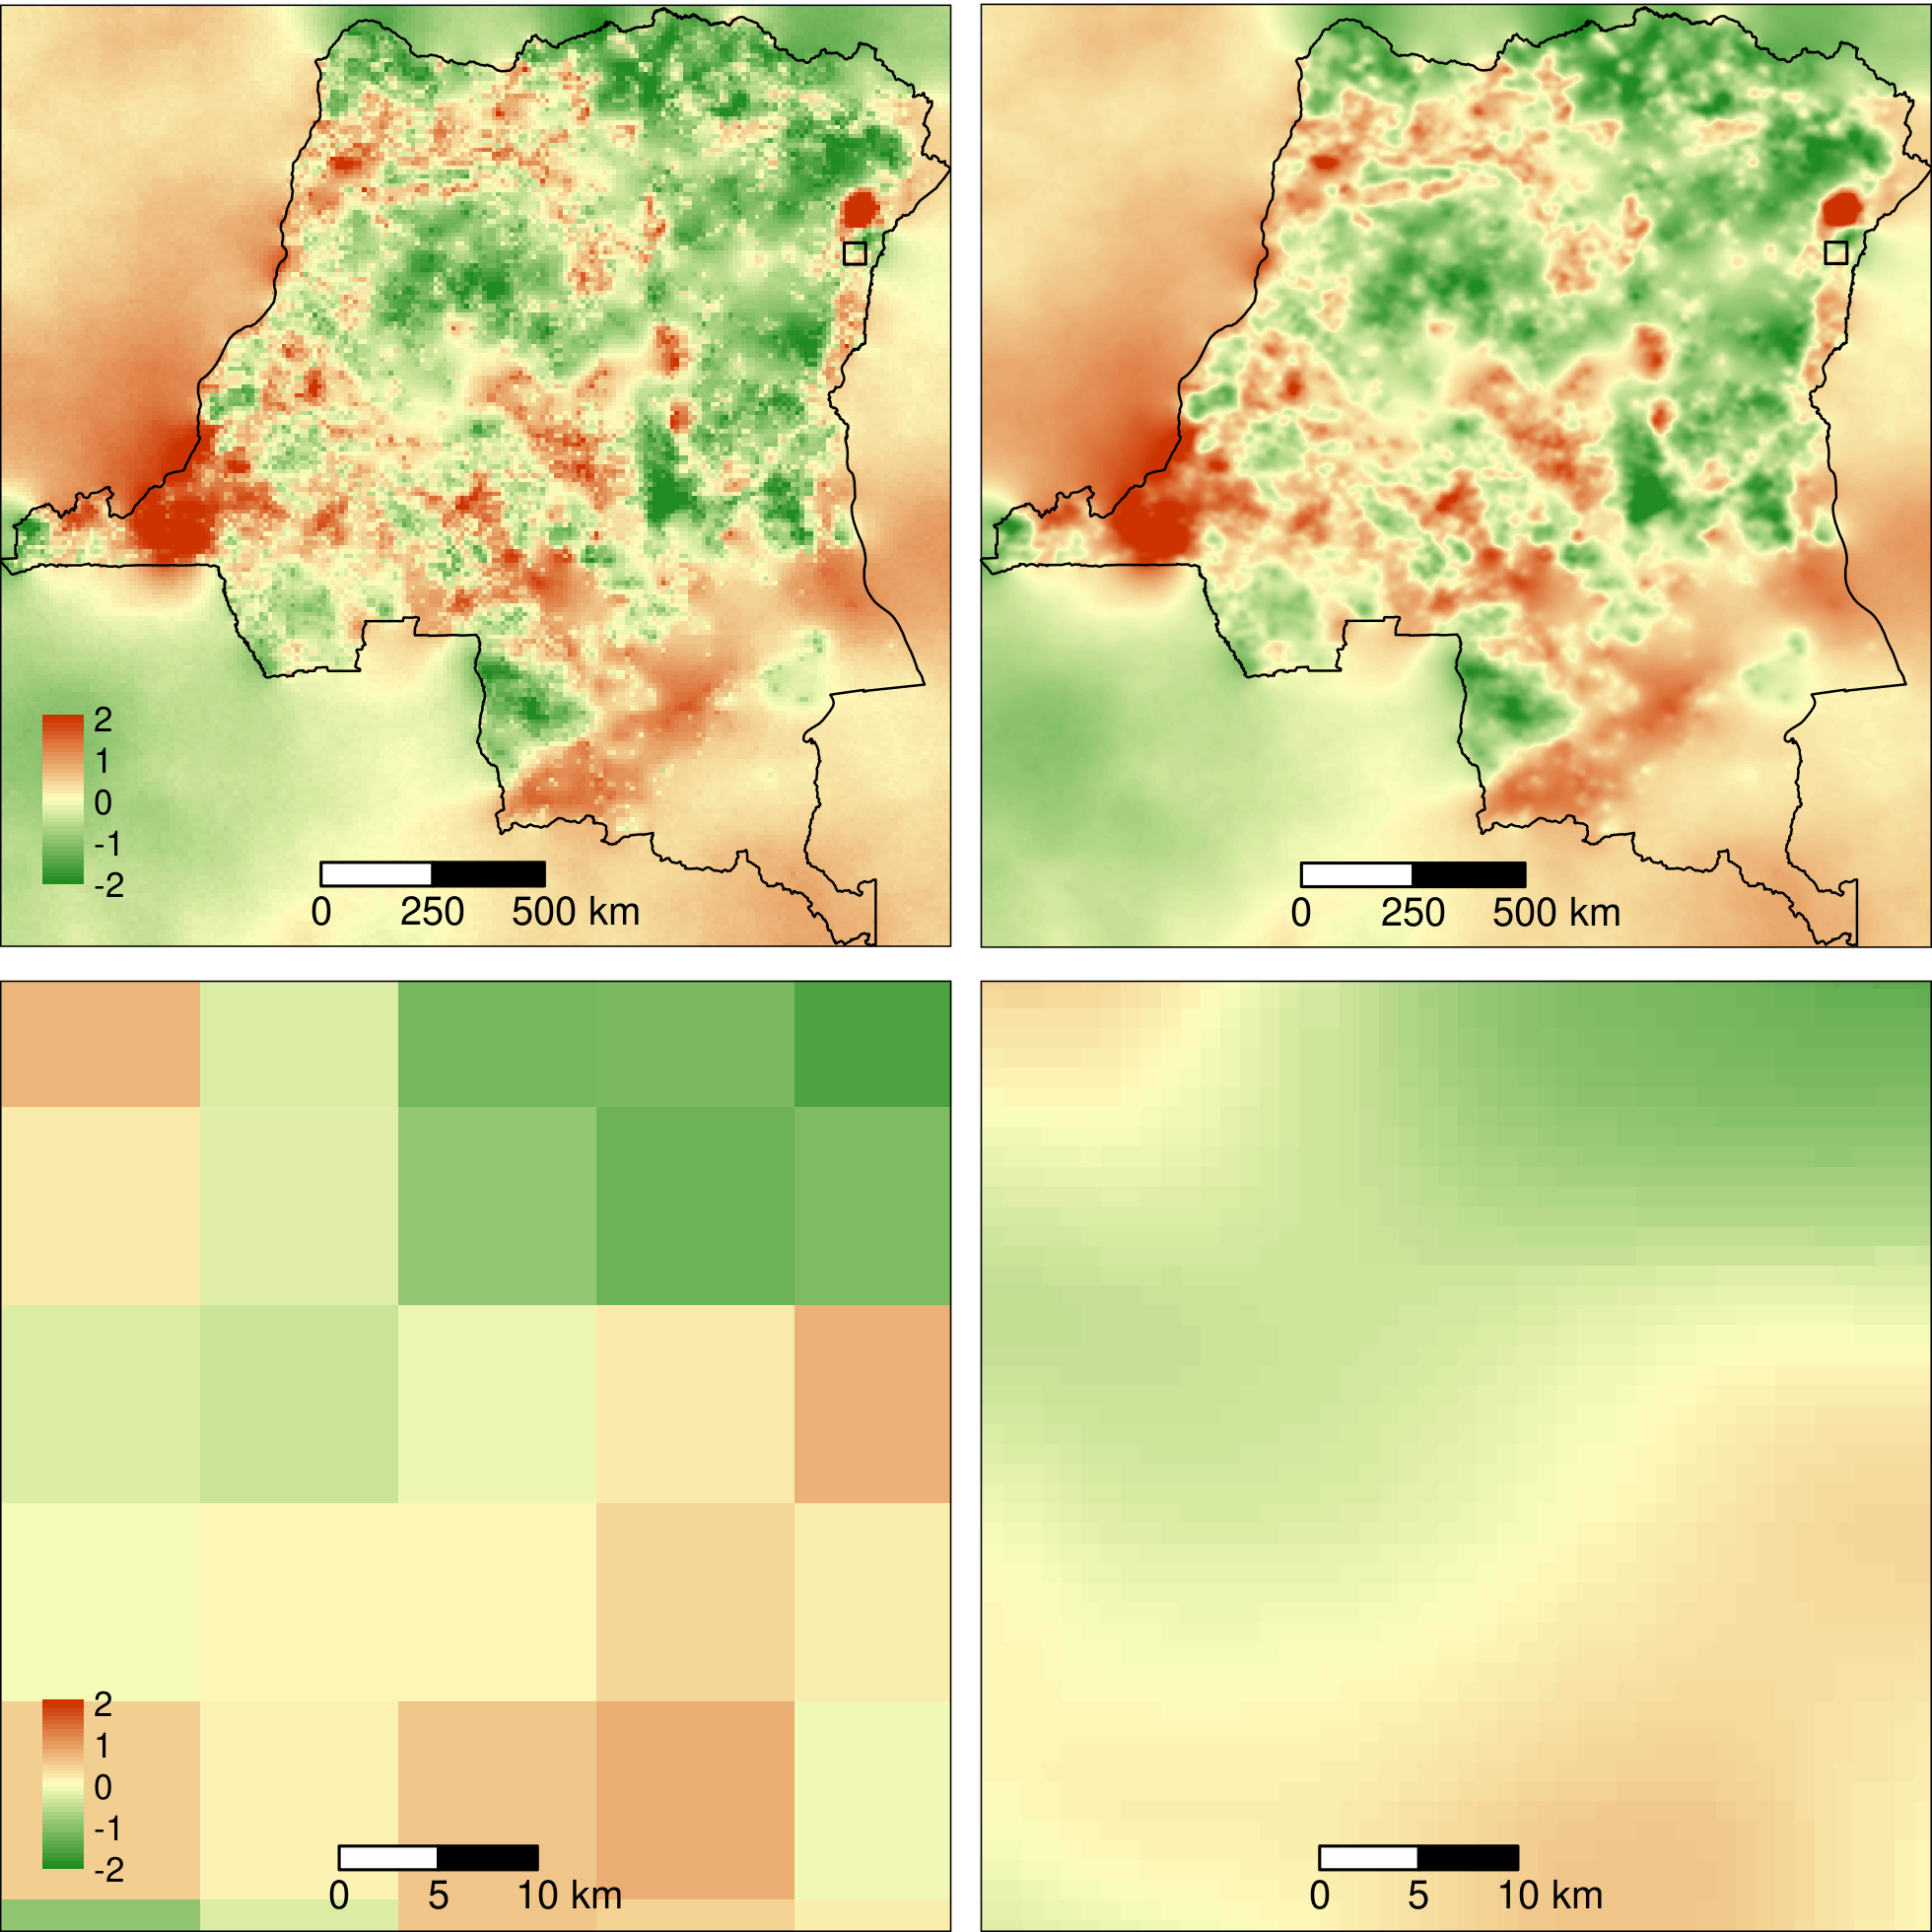
\includegraphics[width=\textwidth]{figs_sm/rho} 

}

\caption{\textbf{Estimated spatial random effects}. \emph{Left}: Estimated spatial random effects at 10 km resolution for the Democratic Republic of the Congo (DRC). \emph{Right}: Interpolated spatial random effects at 1 km resolution. A bicubic interpolation method was used. \emph{Bottom}: Zoom for an area at the North-East of the country (black square) which is close to the city of Beni and the Virunga national park. Due to the structure of the intrinsic CAR model (see Eq.~\eqref{eq:icar}), spatial random effects are also estimated for cells without sampled points. This includes cells for which there was no forest cover in the period 2000--2010--2020, and also cells outside the country's borders.}\label{fig:rho}
\end{figure}

\hypertarget{relative-spatial-probability-of-deforestation}{%
\subsection{Relative spatial probability of deforestation}\label{relative-spatial-probability-of-deforestation}}



\begin{figure}[H]

{\centering 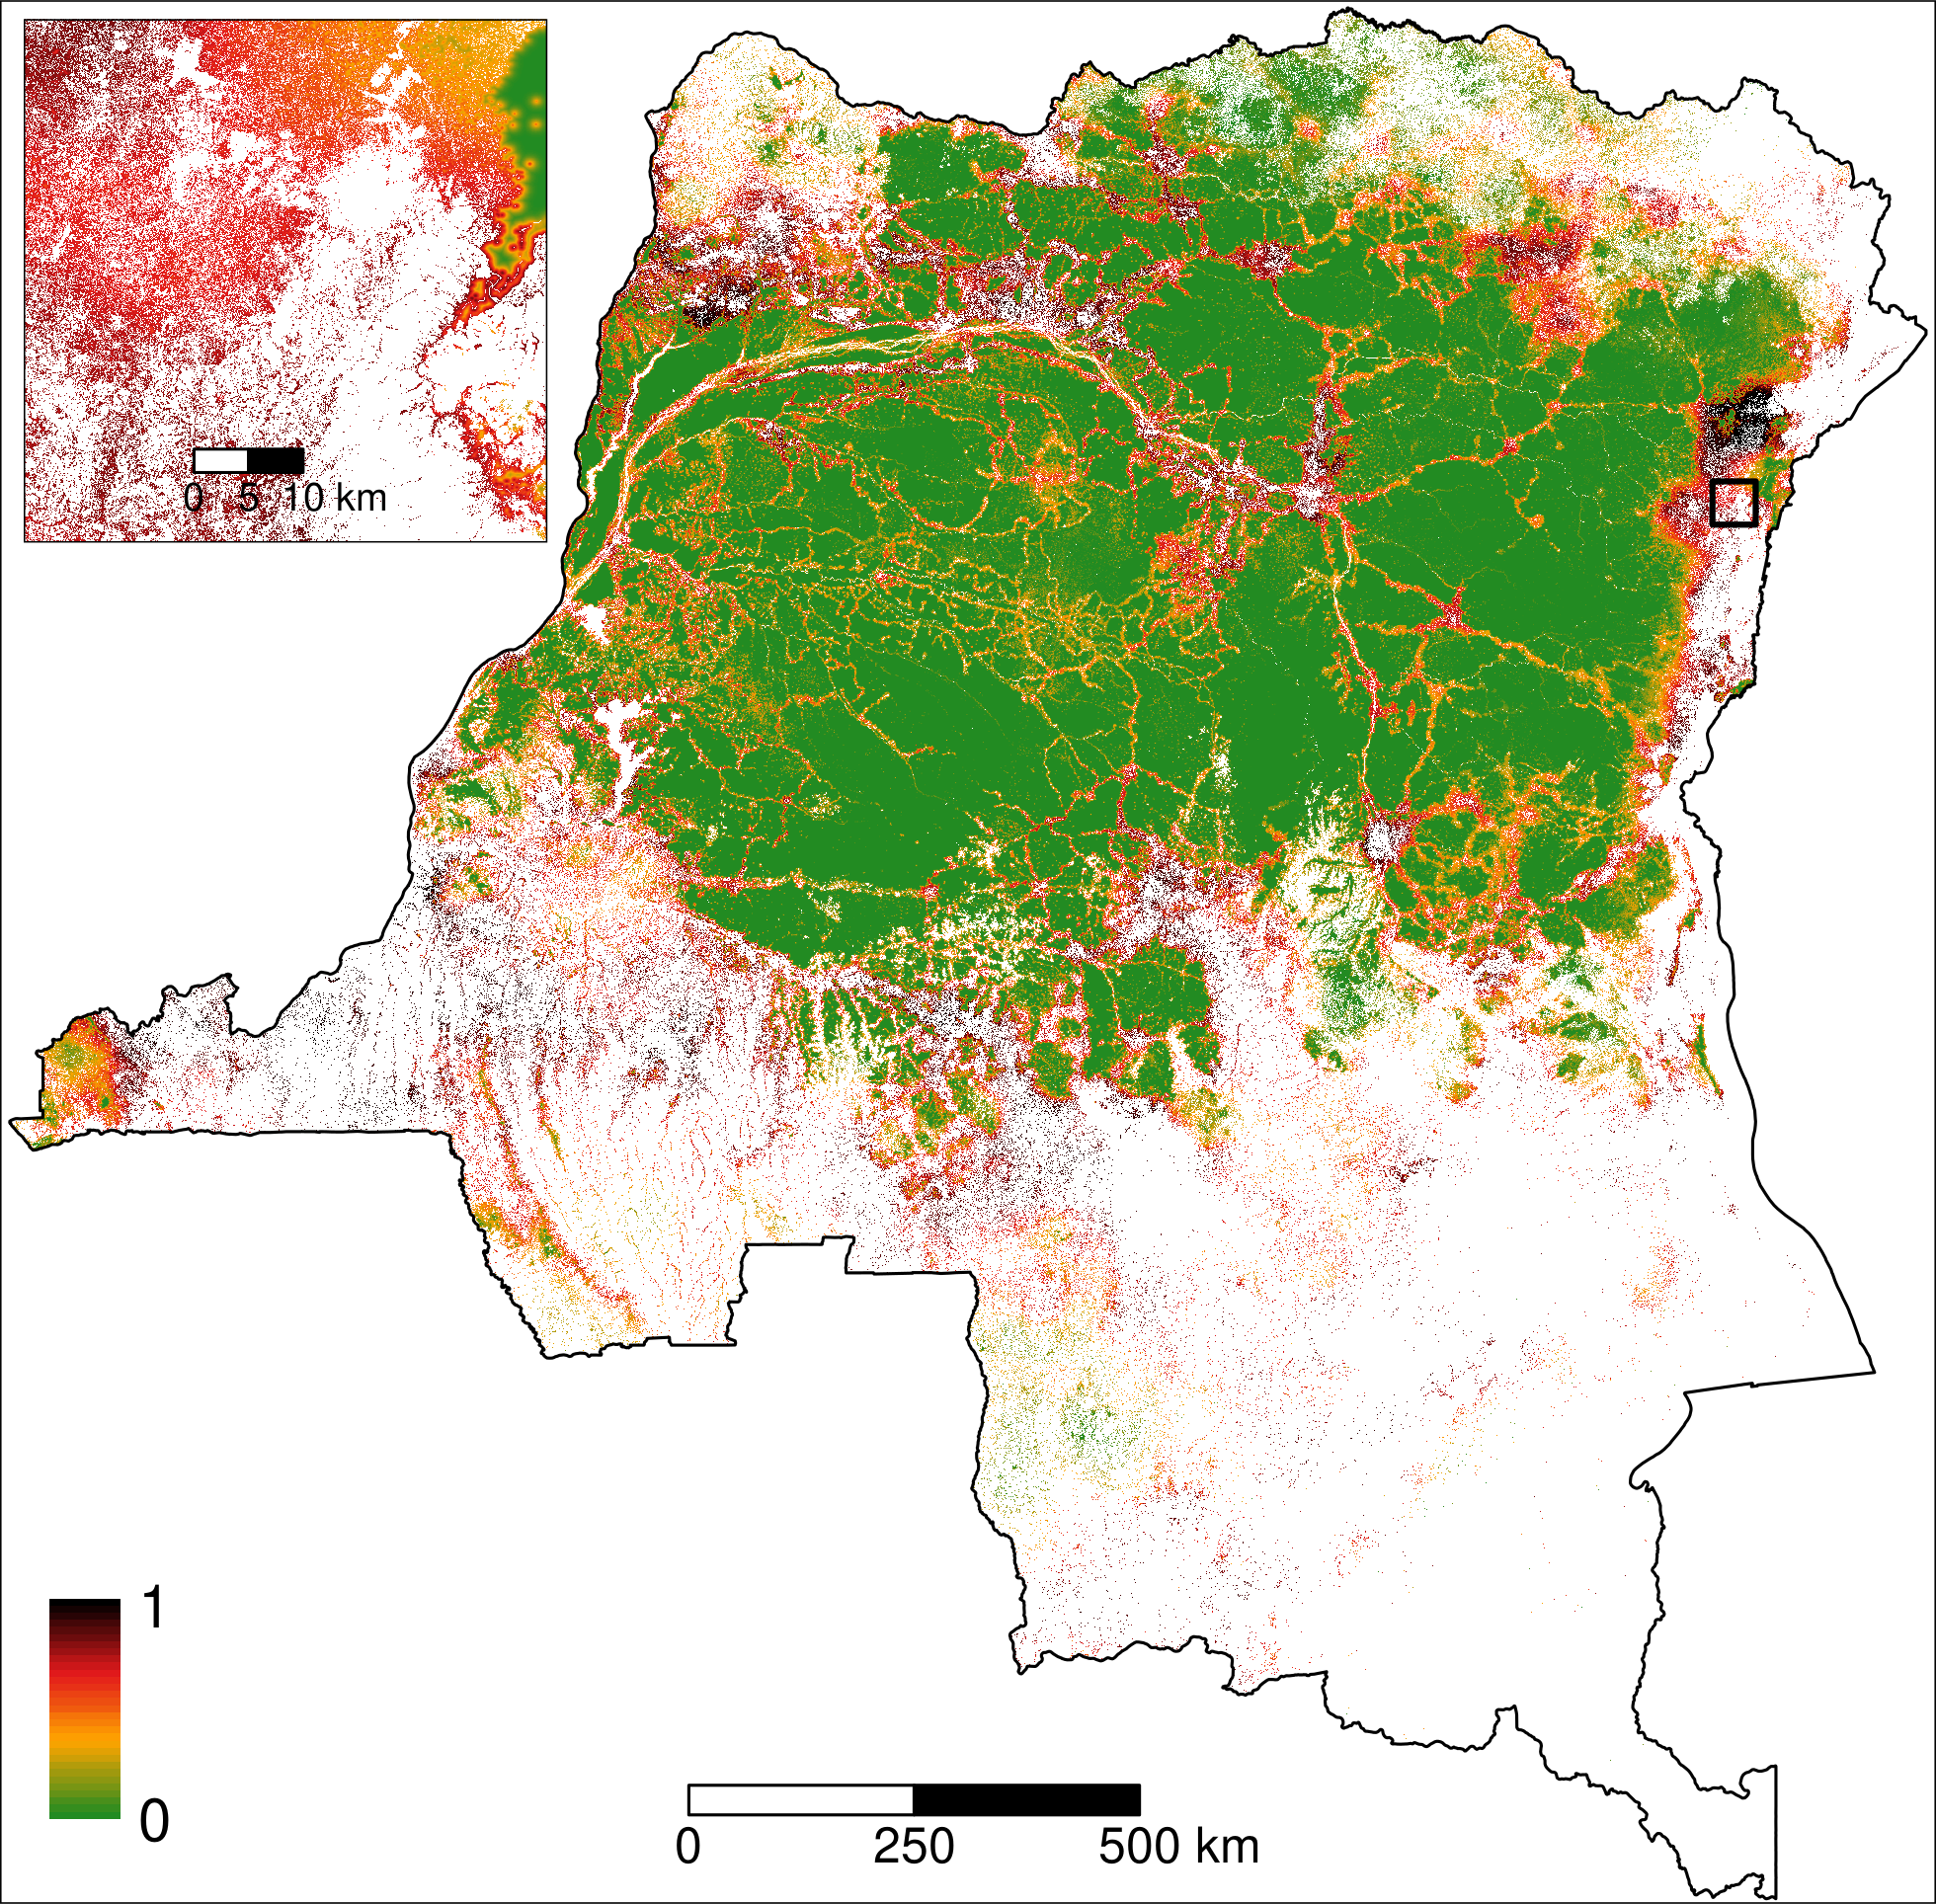
\includegraphics[width=0.98\textwidth]{figs_sm/prob} 

}

\caption{\textbf{Predicted relative spatial probability of deforestation}. \emph{Main figure}: Map of the spatial probability of deforestation computed for each forest pixel in 2020 for the Democratic Republic of the Congo. On the map, we clearly see the effect of the distance to nearest town and road, and the effect of the distance to forest edge on the spatial probability of deforestation. Also, we clearly see the importance of the spatial random effects in structuring the spatial variability of the deforestation probability. For example, the area at the North of the zoom (black square) shows very high deforestation probabilities (in black). This area is politically unstable and is home to a large number of militias who survive at the expense of the forest. \emph{Inset}: Zoom of the map for an area at the North-East of the country which is close to the city of Beni and the Virunga national park. An interactive global map of the spatial probability of deforestation is available at \url{https://forestatrisk.cirad.fr/maps.html}.}\label{fig:sm-prob}
\end{figure}

\hypertarget{projected-forest-cover-change}{%
\subsection{Projected forest cover change}\label{projected-forest-cover-change}}



\begin{figure}[H]

{\centering 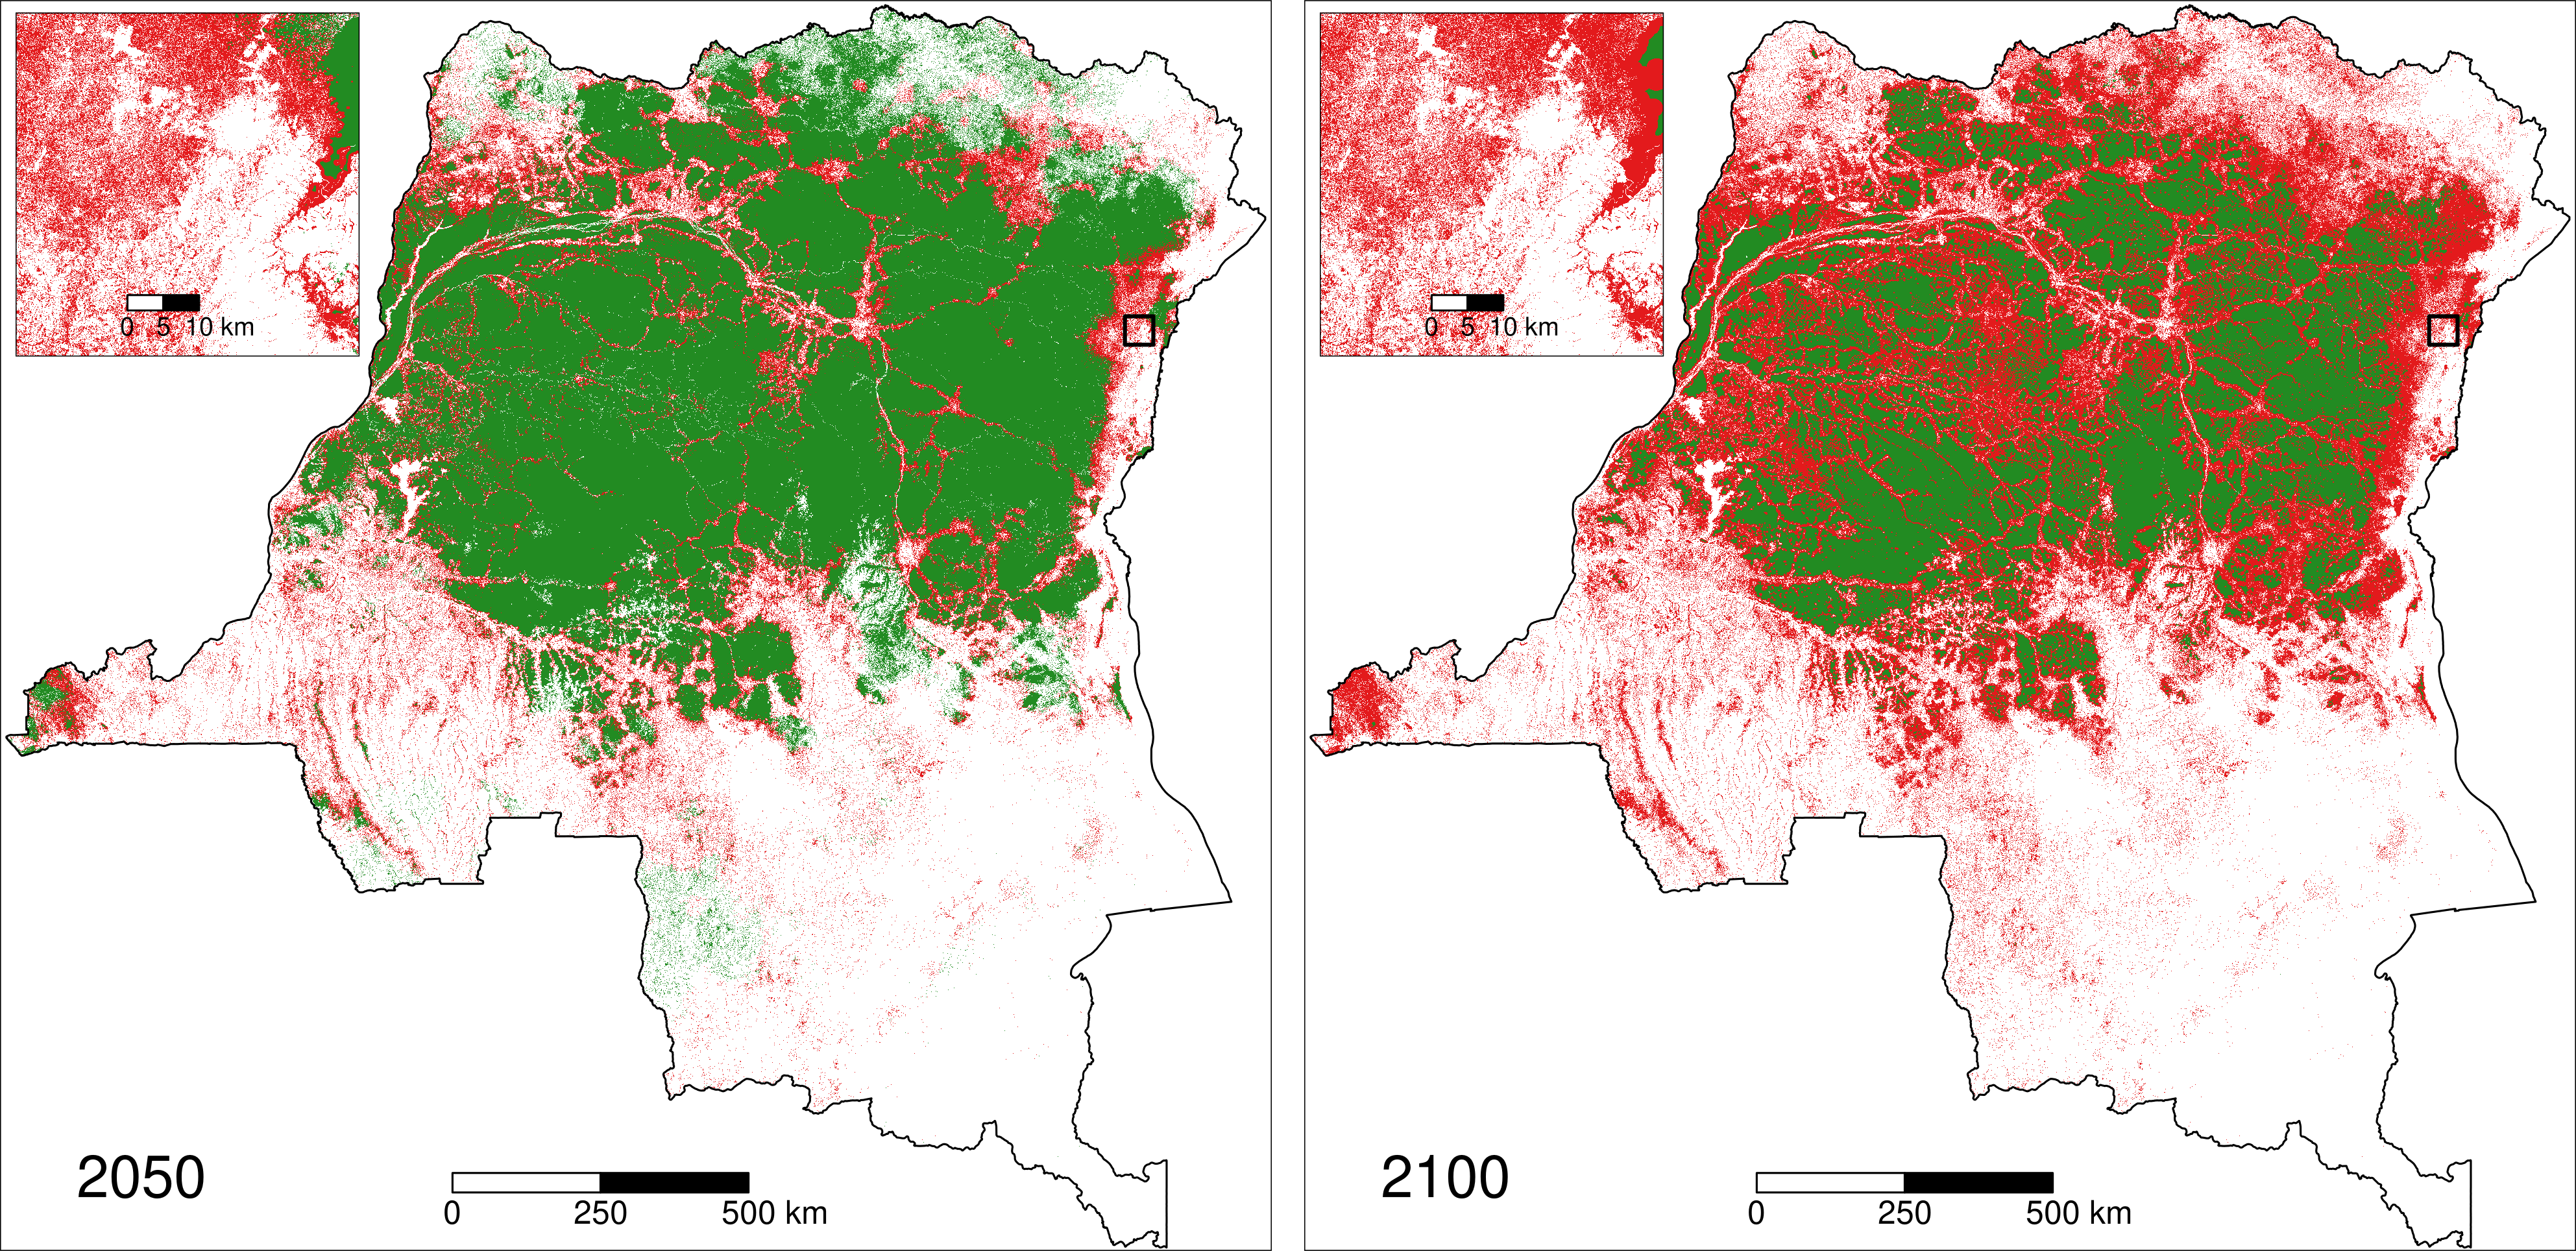
\includegraphics[width=\textwidth]{figs_sm/fcc2050_2100} 

}

\caption{\textbf{Projected forest cover change}. \emph{Main figures}: Maps of the projected forest cover change (left: 2020--2050, right: 2020--2100) for the Democratic Republic of the Congo (DRC). \textcolor{red}{red}: projected deforestation, \textcolor{darkgreen}{green}: remaining forest cover. Besides the loss of forest cover, we show a progressive fragmentation of the forest in the future, with an increasing number of forest patches of smaller size in DRC. \emph{Insets}: Zoom of the map for an area at the North-East of the country (black square) which is close to the city of Beni and the Virunga national park. Interactive global maps of the projected forest cover change for years 2050 and 2100 are available at \url{https://forestatrisk.cirad.fr/maps.html}.}\label{fig:sm-proj}
\end{figure}

\hypertarget{aboveground-biomass-map}{%
\subsection{Aboveground biomass map}\label{aboveground-biomass-map}}



\begin{figure}[H]

{\centering 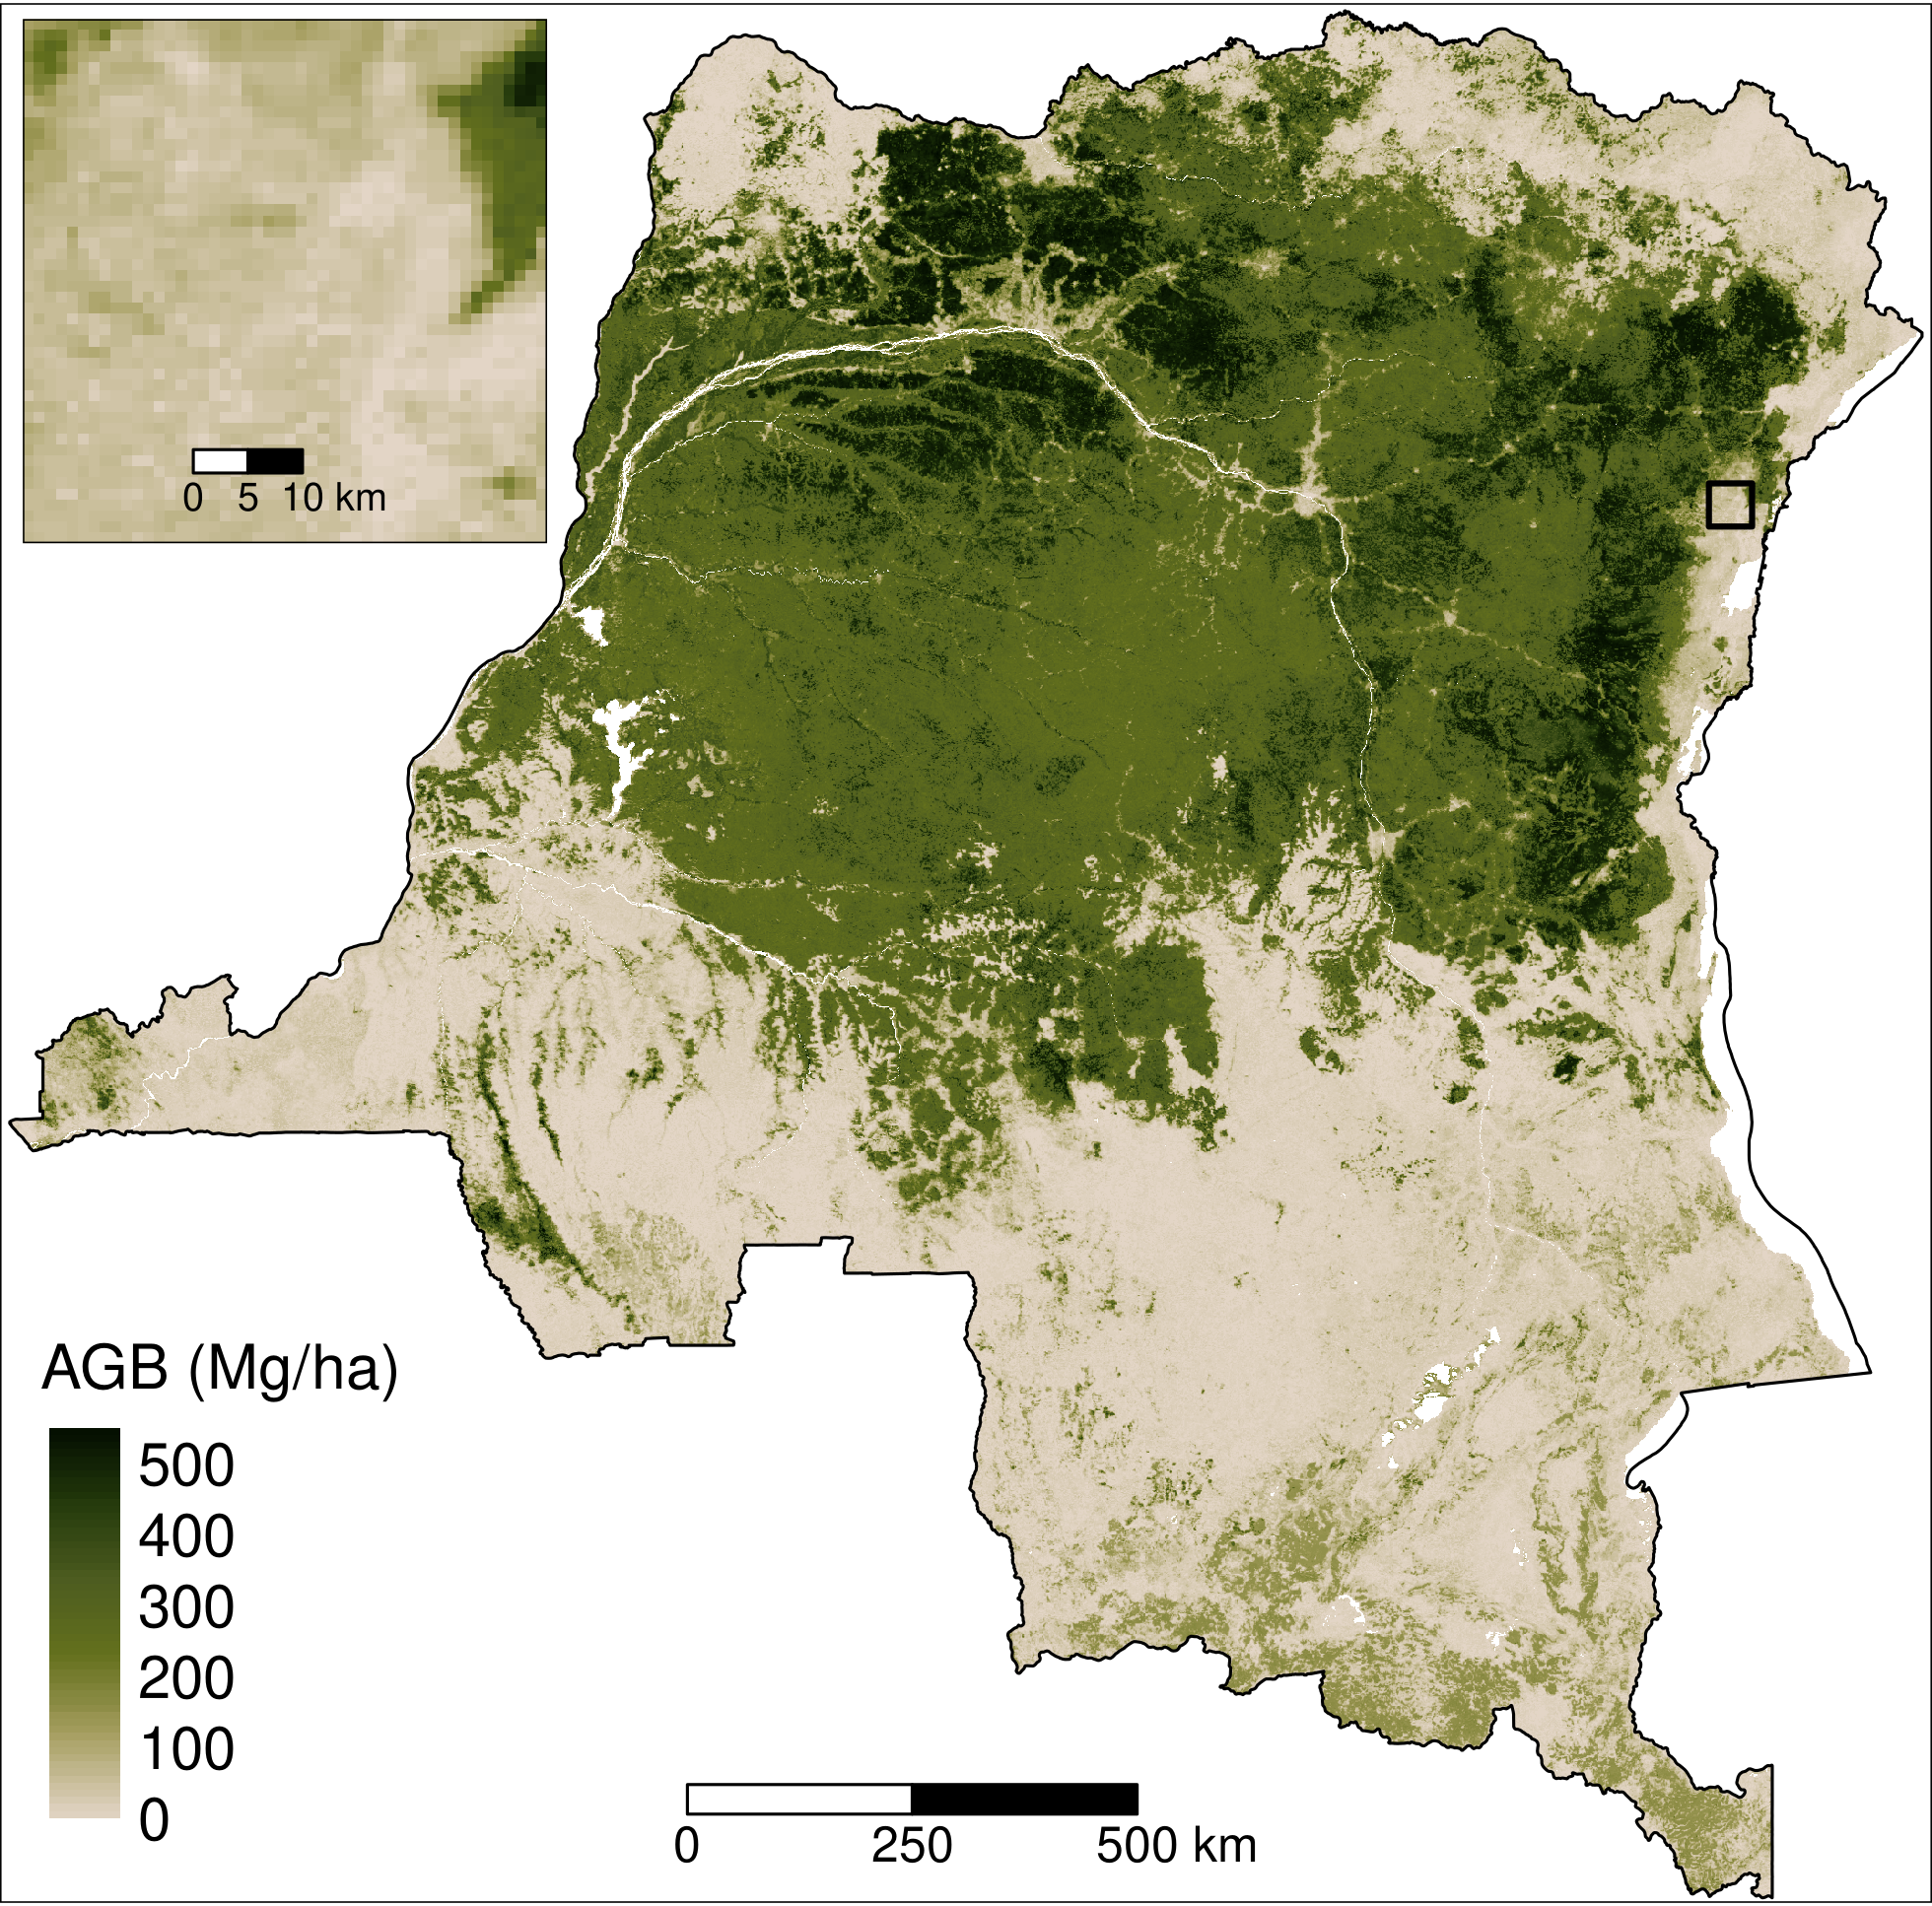
\includegraphics[width=\textwidth]{figs_sm/AGB} 

}

\caption{\textbf{Aboveground biomass map}. \emph{Main figure}: Aboveground biomass (AGB in Mg/ha) map for the Democratic Republic of the Congo (DRC) at 1~km resolution produced by Avitabile \emph{et al.} \citep{Avitabile2016}. This map is a combination of two pantropical aboveground biomass maps by Saatchi \emph{et al.} \citep{Saatchi2011} and Baccini \emph{et al.} \citep{Baccini2012}. While the RMSE of the fused map by Avitabile \emph{et al.} \citep{Avitabile2016} is still substantial (87--98 Mg/ha), the fused map achieved a lower RMSE (a decrease of 5--74\%) and bias (a decrease of 90--153\%) than the two input maps for all continents. The fusion map is representative of the aboveground biomass for the years 2000--2010. \emph{Inset}: Zoom of the map for an area at the North-East of the country which is close to the city of Beni and the Virunga national park.}\label{fig:agb}
\end{figure}

\hypertarget{uncertainty-map-of-the-future-change-in-forest-cover}{%
\subsection{Uncertainty map of the future change in forest cover}\label{uncertainty-map-of-the-future-change-in-forest-cover}}



\begin{figure}[H]

{\centering 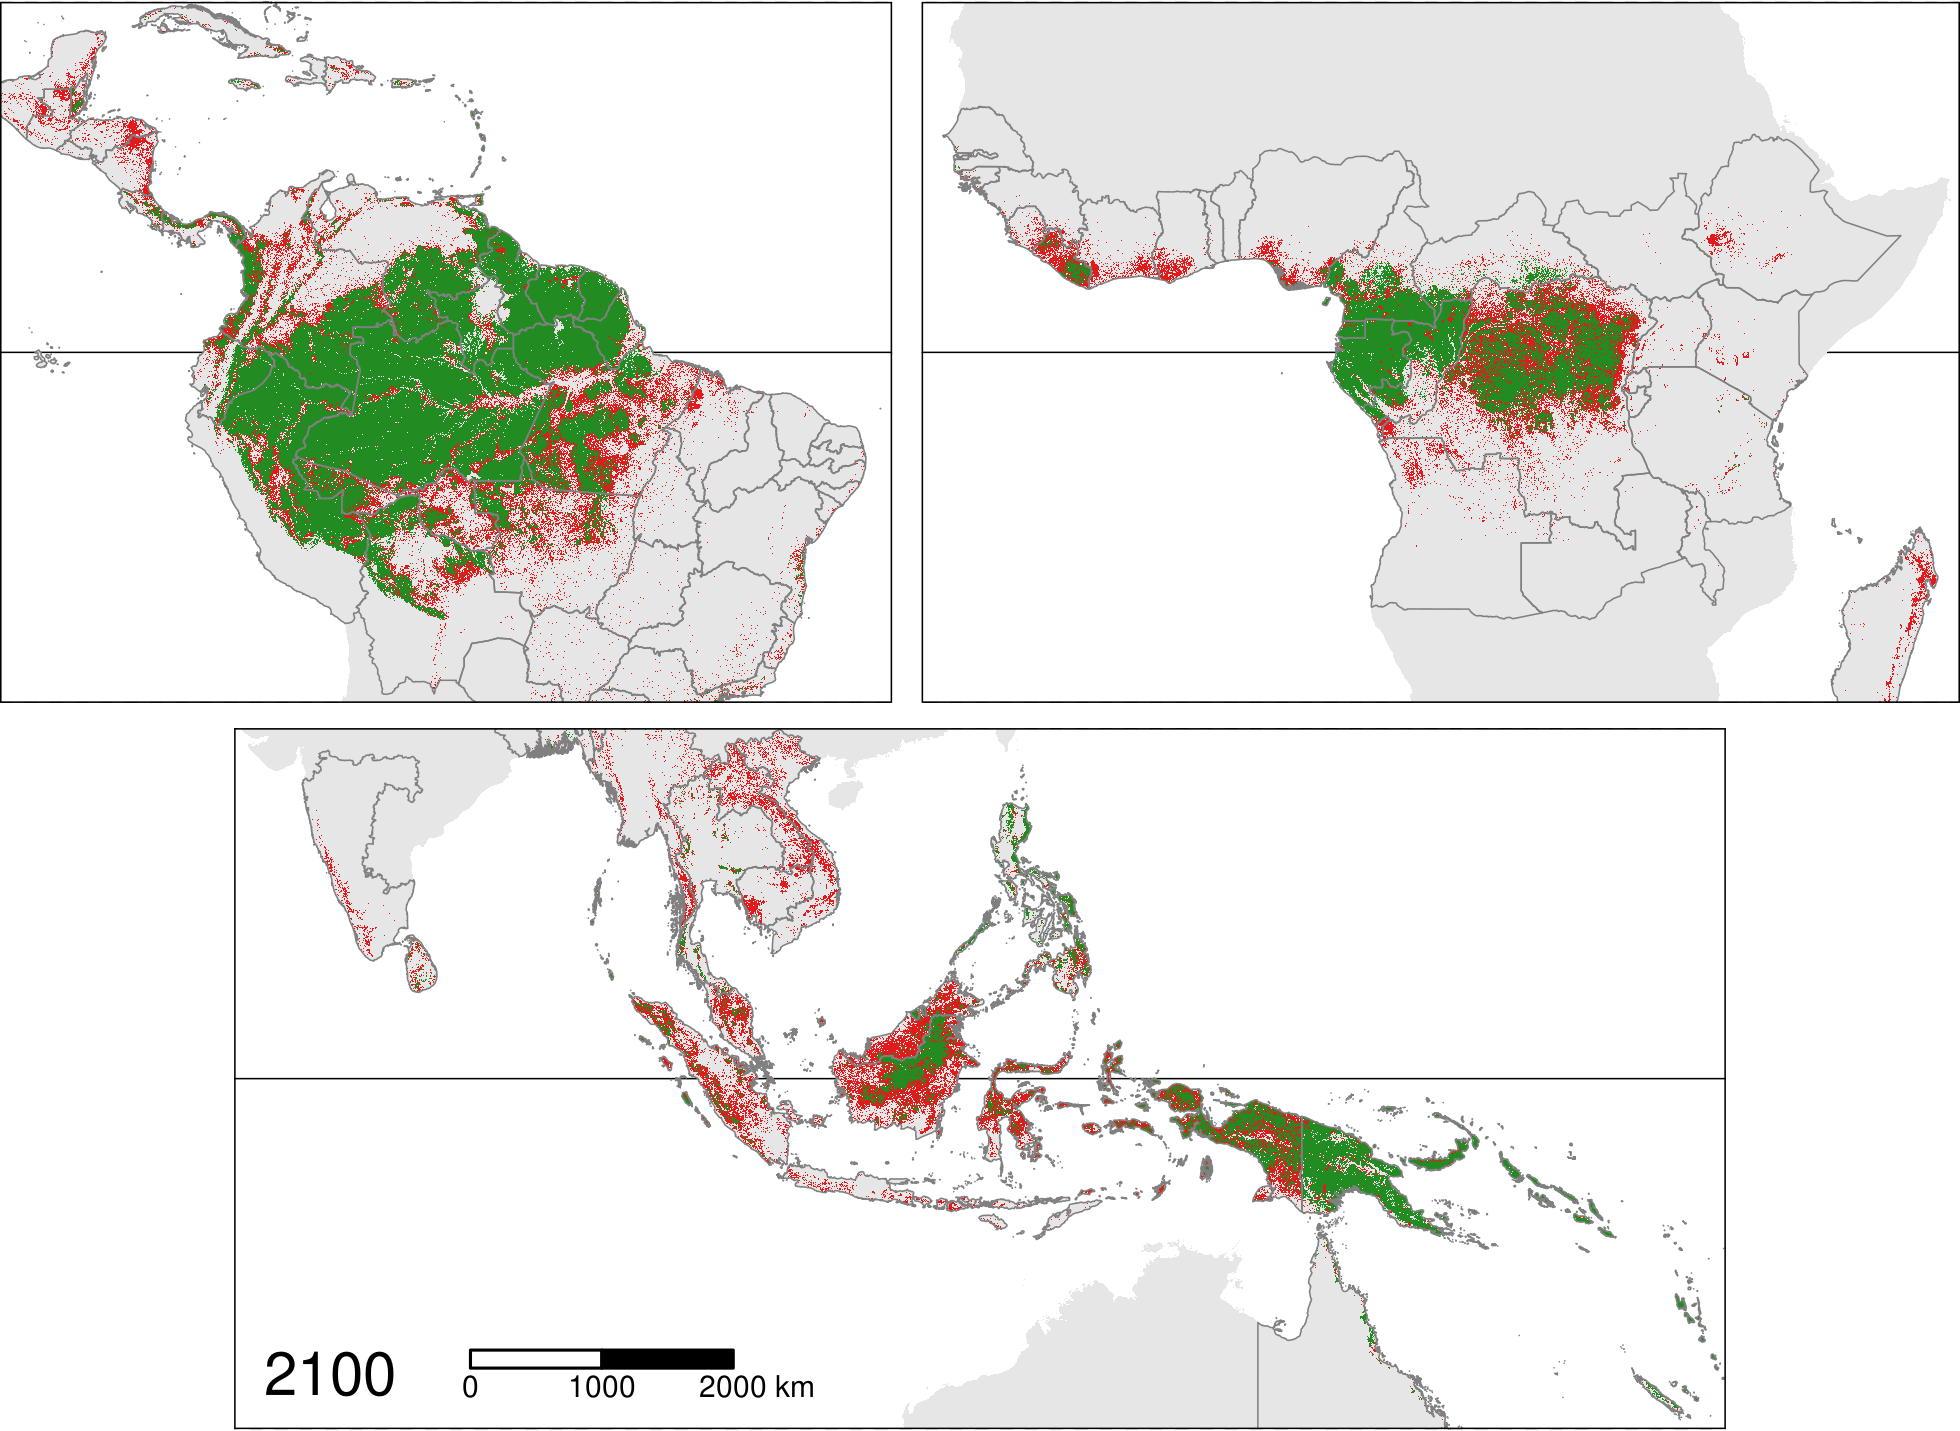
\includegraphics[width=\textwidth]{figs_sm/fcc2100_min} 

}

\caption{\textbf{Projected forest cover change map assuming a low annual deforestation}. This map was derived using \(d'\), the \emph{lower} limit of the confidence interval for the annual deforested area (in ha/yr) for each study area. This map must be compared with Fig.~1 in the main text and Fig.~\ref{fig:fcc2100-high} below, which consider average and high annual deforestation, respectively. The horizontal black line indicates the position of the Equator. The boundaries of the study areas are represented by dark grey lines. Forest areas in \textcolor{red}{red} are predicted to be deforested during the period 2020--2100, while forest areas in \textcolor{darkgreen}{green} are predicted to remain in 2100.}\label{fig:fcc2100-low}
\end{figure}



\begin{figure}[H]

{\centering 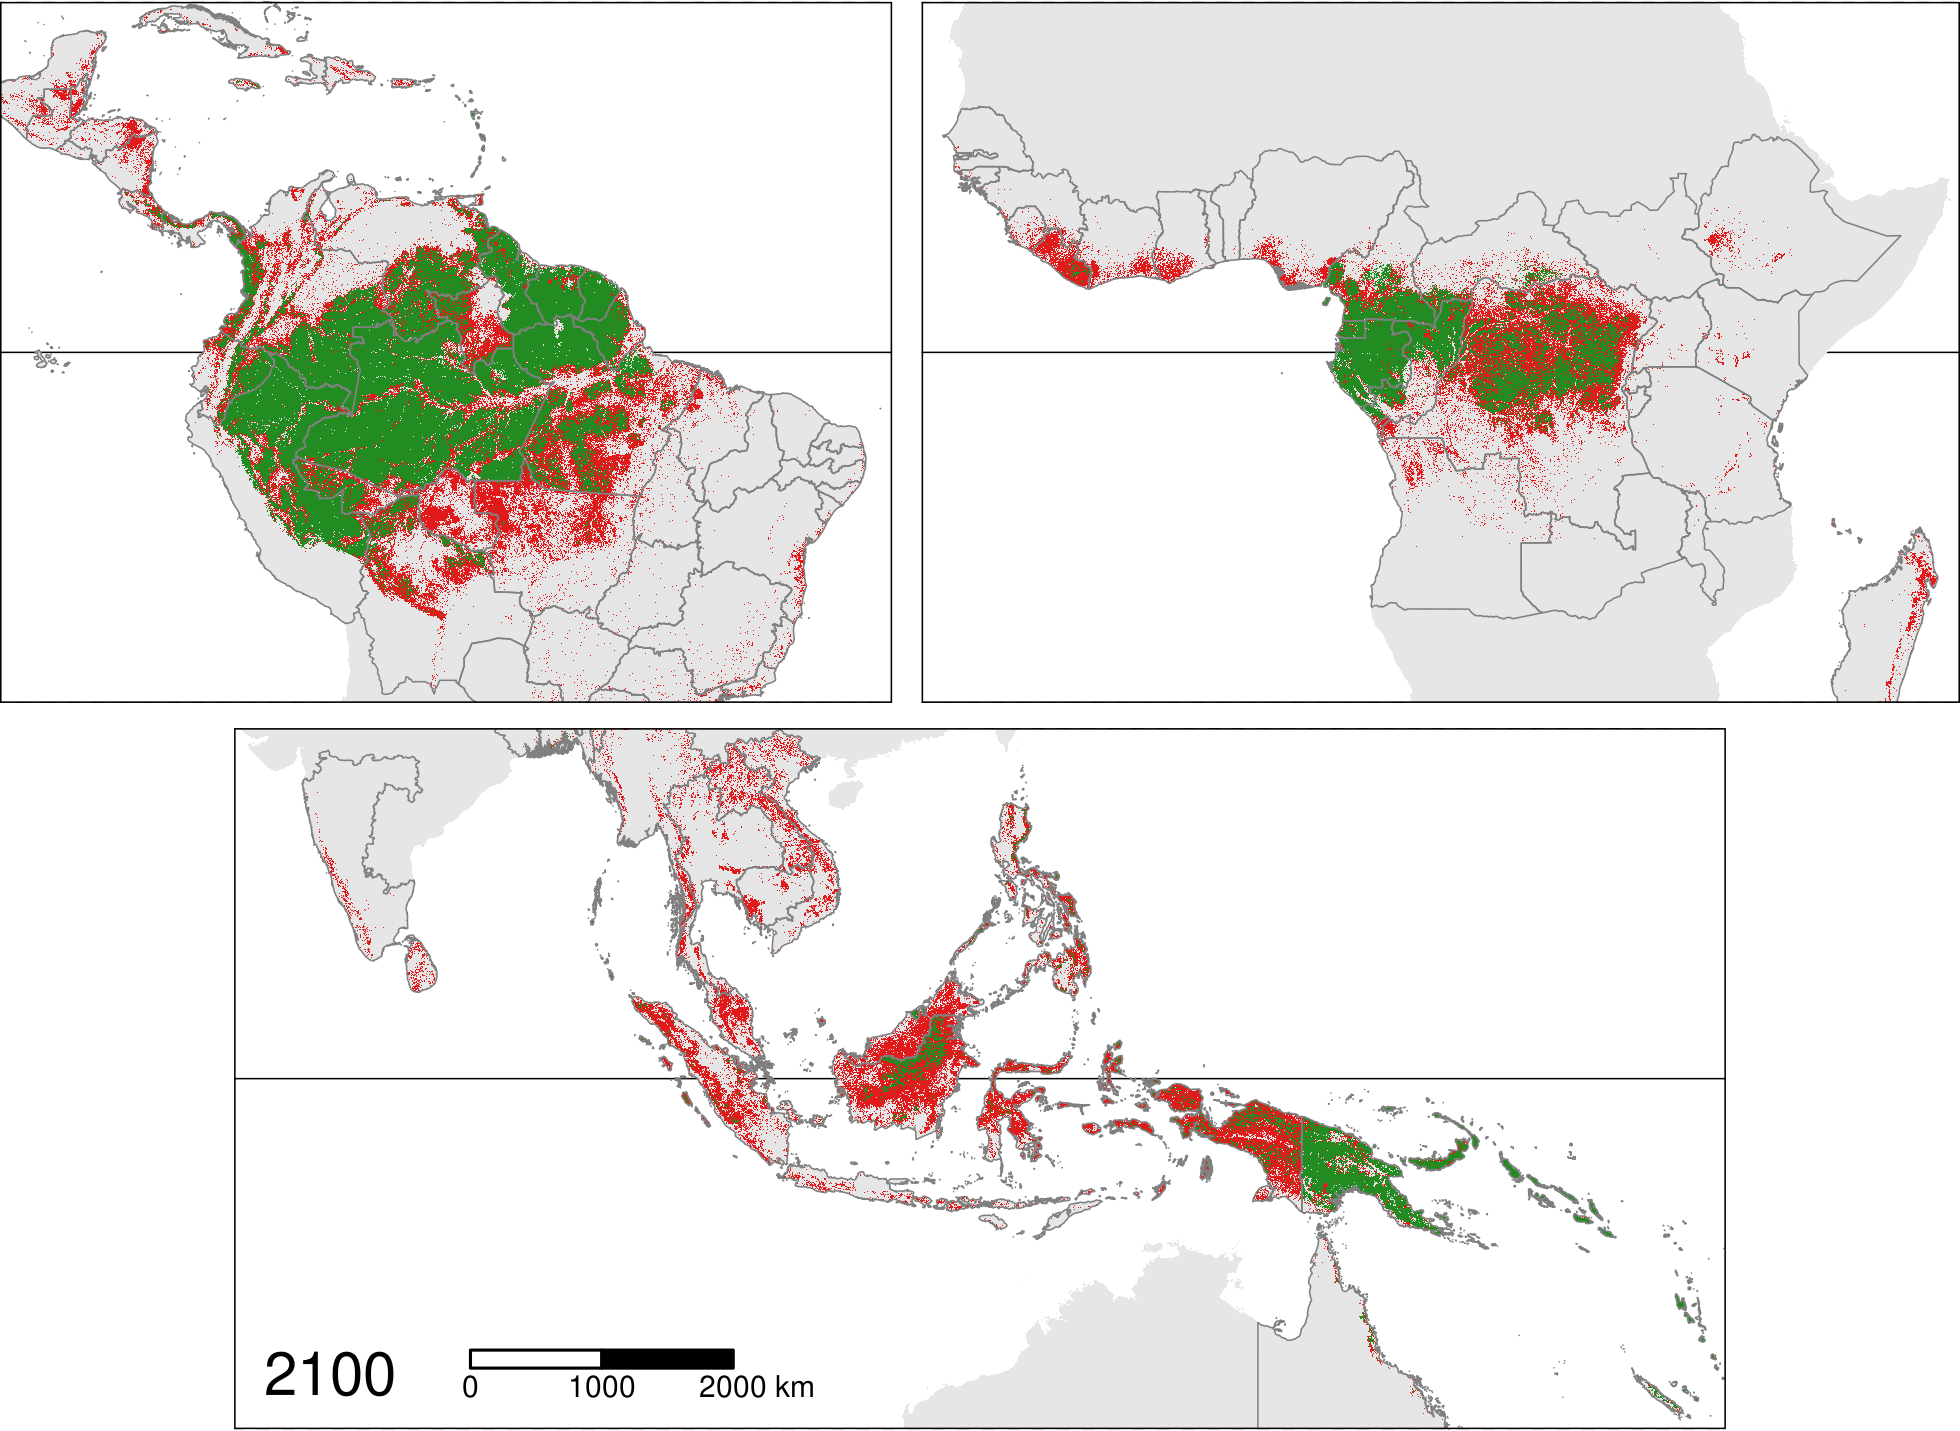
\includegraphics[width=\textwidth]{figs_sm/fcc2100_max} 

}

\caption{\textbf{Projected forest cover change map assuming a high annual deforestation}. This map was derived using \(d''\), the \emph{upper} limit of the confidence interval for the annual deforested area (in ha/yr) for each study area. This map must be compared with Fig.~1 in the main text and Fig.~\ref{fig:fcc2100-low} above, which consider average and low annual deforestation, respectively. The horizontal black line indicates the position of the Equator. The boundaries of the study areas are represented by dark grey lines. Forest areas in \textcolor{red}{red} are predicted to be deforested in the period 2020--2100, while forest areas in \textcolor{darkgreen}{green} are predicted to remain in 2100.}\label{fig:fcc2100-high}
\end{figure}

\newpage

\hypertarget{supplementary-tables}{%
\section{Supplementary tables}\label{supplementary-tables}}

\hypertarget{categories-of-the-forest-cover-annual-product}{%
\subsection{Categories of the forest cover annual product}\label{categories-of-the-forest-cover-annual-product}}



\begin{table}[H]

\caption{\label{tab:cat-annual-product}\textbf{Categories of the forest cover annual product by Vancutsem \emph{et al.} \citep{Vancutsem2021}}. The forest cover annual product classifies Landsat image pixels in 6 categories for each year (on the 31\(^{\text{st}}\) of December) between 1990 and 2019 and allows identifying moist tropical forest pixels at each date.\vspace{0.5cm}}
\centering
\begin{tabular}[t]{>{\raggedright\arraybackslash}p{2cm}>{\raggedleft\arraybackslash}p{10cm}}
\toprule
Class & Definition\\
\midrule
\cellcolor{gray!6}{1} & \cellcolor{gray!6}{Undisturbed Tropical Moist Forest (TMF)}\\
2 & Degraded TMF\\
\cellcolor{gray!6}{3} & \cellcolor{gray!6}{Deforested land}\\
4 & Forest regrowth\\
\cellcolor{gray!6}{5} & \cellcolor{gray!6}{Permanent or seasonal water}\\
6 & Other land cover\\
\bottomrule
\end{tabular}
\end{table}

\hypertarget{variables}{%
\subsection{Variables}\label{variables}}



\begin{table}[H]

\caption{\label{tab:variables}\textbf{Set of explicative variables used to model the spatial probability of deforestation}. A total of height variables were tested. They indicate topography, forest accessibility, forest landscape, deforestation history, and conservation status.\vspace{0.5cm}}
\centering
\fontsize{11}{13}\selectfont
\begin{tabular}[t]{>{\raggedright\arraybackslash}p{2.5cm}>{\raggedright\arraybackslash}p{2.5cm}>{\raggedright\arraybackslash}p{2.5cm}>{\raggedleft\arraybackslash}p{1cm}>{\raggedleft\arraybackslash}p{2cm}>{\raggedleft\arraybackslash}p{2cm}}
\toprule
Product & Source & Variable derived & Unit & Resolution (m) & Date\\
\midrule
\cellcolor{gray!6}{Forest maps (2000-2010-2020)} & \cellcolor{gray!6}{Vancutsem et al. 2021} & \cellcolor{gray!6}{distance to forest edge} & \cellcolor{gray!6}{m} & \cellcolor{gray!6}{30} & \cellcolor{gray!6}{--}\\
 &  & distance to past deforestation & m & 30 & --\\
\cellcolor{gray!6}{Digital Elevation Model} & \cellcolor{gray!6}{SRTM v4.1 CSI-CGIAR} & \cellcolor{gray!6}{elevation} & \cellcolor{gray!6}{m} & \cellcolor{gray!6}{90} & \cellcolor{gray!6}{--}\\
 &  & slope & degree & 90 & --\\
\cellcolor{gray!6}{Highways} & \cellcolor{gray!6}{OSM-Geofabrik} & \cellcolor{gray!6}{distance to road} & \cellcolor{gray!6}{m} & \cellcolor{gray!6}{150} & \cellcolor{gray!6}{March 2021}\\
Places &  & distance to town & m & 150 & March 2021\\
\cellcolor{gray!6}{Waterways} & \cellcolor{gray!6}{} & \cellcolor{gray!6}{distance to river} & \cellcolor{gray!6}{m} & \cellcolor{gray!6}{150} & \cellcolor{gray!6}{March 2021}\\
Protected areas & WDPA & presence of protected area & -- & 30 & March 2021\\
\bottomrule
\end{tabular}
\end{table}

\newpage

\hypertarget{sample-size}{%
\subsection{Sample size}\label{sample-size}}



\begingroup\fontsize{11}{13}\selectfont

\begin{longtable}[t]{llrrrr}
\caption{\label{tab:samp-size}\textbf{Number of observations used for the spatial model of deforestation for each study area}. The table includes the number of non-deforested (nfor) and deforested (ndef) pixels per study area. These numbers include the forest pixels with full information regarding the explanatory variables. The corresponding number of hectares is also provided (nfHa and ndHa, respectively).\vspace{0.5cm}}\\
\toprule
\multicolumn{1}{l}{Country -- Study area} & \multicolumn{1}{l}{Code} & \multicolumn{1}{r}{nfor} & \multicolumn{1}{r}{ndef} & \multicolumn{1}{r}{nfHa} & \multicolumn{1}{r}{ndHa} \\
 &  &  &  & (ha) & (ha)\\
\midrule
\endfirsthead
\caption[]{\textit{(continued)}}\\
\toprule
\multicolumn{1}{l}{Country -- Study area} & \multicolumn{1}{l}{Code} & \multicolumn{1}{r}{nfor} & \multicolumn{1}{r}{ndef} & \multicolumn{1}{r}{nfHa} & \multicolumn{1}{r}{ndHa} \\
 &  &  &  & (ha) & (ha)\\
\midrule
\endhead

\endfoot
\bottomrule
\endlastfoot
\addlinespace[0.3em]
\multicolumn{6}{l}{\textbf{America}}\\
\cellcolor{gray!6}{\hspace{1em}Antigua and B.} & \cellcolor{gray!6}{ATG} & \cellcolor{gray!6}{9,858} & \cellcolor{gray!6}{5,771} & \cellcolor{gray!6}{887} & \cellcolor{gray!6}{519}\\
\hspace{1em}Bahamas & BHS & 9,898 & 9,953 & 891 & 896\\
\cellcolor{gray!6}{\hspace{1em}Barbados} & \cellcolor{gray!6}{BRB} & \cellcolor{gray!6}{9,960} & \cellcolor{gray!6}{7,816} & \cellcolor{gray!6}{896} & \cellcolor{gray!6}{703}\\
\hspace{1em}Belize & BLZ & 9,992 & 9,998 & 899 & 900\\
\cellcolor{gray!6}{\hspace{1em}Bolivia} & \cellcolor{gray!6}{BOL} & \cellcolor{gray!6}{30,657} & \cellcolor{gray!6}{30,657} & \cellcolor{gray!6}{2,759} & \cellcolor{gray!6}{2,759}\\
\hspace{1em}Brazil – Acre & AC & 13,292 & 13,292 & 1,196 & 1,196\\
\cellcolor{gray!6}{\hspace{1em}Brazil – Alagoas} & \cellcolor{gray!6}{AL} & \cellcolor{gray!6}{9,997} & \cellcolor{gray!6}{9,997} & \cellcolor{gray!6}{900} & \cellcolor{gray!6}{900}\\
\hspace{1em}Brazil – Amapa & AP & 11,587 & 11,589 & 1,043 & 1,043\\
\cellcolor{gray!6}{\hspace{1em}Brazil – Amazonas} & \cellcolor{gray!6}{AM} & \cellcolor{gray!6}{50,000} & \cellcolor{gray!6}{50,000} & \cellcolor{gray!6}{4,500} & \cellcolor{gray!6}{4,500}\\
\hspace{1em}Brazil – Bahia & BA & 9,997 & 9,999 & 900 & 900\\
\cellcolor{gray!6}{\hspace{1em}Brazil – Ceara} & \cellcolor{gray!6}{CE} & \cellcolor{gray!6}{9,996} & \cellcolor{gray!6}{9,999} & \cellcolor{gray!6}{900} & \cellcolor{gray!6}{900}\\
\hspace{1em}Brazil – Espirito Santo & ES & 9,996 & 9,997 & 900 & 900\\
\cellcolor{gray!6}{\hspace{1em}Brazil – Goias} & \cellcolor{gray!6}{GO} & \cellcolor{gray!6}{10,000} & \cellcolor{gray!6}{10,000} & \cellcolor{gray!6}{900} & \cellcolor{gray!6}{900}\\
\hspace{1em}Brazil – Maranhao & MA & 9,986 & 9,997 & 899 & 900\\
\cellcolor{gray!6}{\hspace{1em}Brazil – Mato Grosso} & \cellcolor{gray!6}{MT} & \cellcolor{gray!6}{33,454} & \cellcolor{gray!6}{33,454} & \cellcolor{gray!6}{3,011} & \cellcolor{gray!6}{3,011}\\
\hspace{1em}Brazil – Mato Grosso do Sul & MS & 10,000 & 10,000 & 900 & 900\\
\cellcolor{gray!6}{\hspace{1em}Brazil – Minas Gerais} & \cellcolor{gray!6}{MG} & \cellcolor{gray!6}{10,000} & \cellcolor{gray!6}{10,000} & \cellcolor{gray!6}{900} & \cellcolor{gray!6}{900}\\
\hspace{1em}Brazil – Para & PA & 49,999 & 50,000 & 4,500 & 4,500\\
\cellcolor{gray!6}{\hspace{1em}Brazil – Paraiba} & \cellcolor{gray!6}{PB} & \cellcolor{gray!6}{9,967} & \cellcolor{gray!6}{9,998} & \cellcolor{gray!6}{897} & \cellcolor{gray!6}{900}\\
\hspace{1em}Brazil – Parana & PR & 9,993 & 10,000 & 899 & 900\\
\cellcolor{gray!6}{\hspace{1em}Brazil – Pernambouco} & \cellcolor{gray!6}{PE} & \cellcolor{gray!6}{9,980} & \cellcolor{gray!6}{9,999} & \cellcolor{gray!6}{898} & \cellcolor{gray!6}{900}\\
\hspace{1em}Brazil – Piaui & PI & 9,999 & 10,000 & 900 & 900\\
\cellcolor{gray!6}{\hspace{1em}Brazil – Rio de Janeiro} & \cellcolor{gray!6}{RJ} & \cellcolor{gray!6}{9,995} & \cellcolor{gray!6}{9,985} & \cellcolor{gray!6}{900} & \cellcolor{gray!6}{899}\\
\hspace{1em}Brazil – Rio Grande do Norte & RN & 9,943 & 9,990 & 895 & 899\\
\cellcolor{gray!6}{\hspace{1em}Brazil – Rio Grande do Sul} & \cellcolor{gray!6}{RS} & \cellcolor{gray!6}{10,000} & \cellcolor{gray!6}{10,000} & \cellcolor{gray!6}{900} & \cellcolor{gray!6}{900}\\
\hspace{1em}Brazil – Rondonia & RO & 13,841 & 13,841 & 1,246 & 1,246\\
\cellcolor{gray!6}{\hspace{1em}Brazil – Roraima} & \cellcolor{gray!6}{RR} & \cellcolor{gray!6}{16,251} & \cellcolor{gray!6}{16,251} & \cellcolor{gray!6}{1,463} & \cellcolor{gray!6}{1,463}\\
\hspace{1em}Brazil – Santa Catarina & SC & 9,996 & 10,000 & 900 & 900\\
\cellcolor{gray!6}{\hspace{1em}Brazil – Sao Paulo} & \cellcolor{gray!6}{SP} & \cellcolor{gray!6}{9,998} & \cellcolor{gray!6}{9,998} & \cellcolor{gray!6}{900} & \cellcolor{gray!6}{900}\\
\hspace{1em}Brazil – Sergipe & SE & 9,982 & 10,000 & 898 & 900\\
\cellcolor{gray!6}{\hspace{1em}Brazil – Tocantins} & \cellcolor{gray!6}{TO} & \cellcolor{gray!6}{10,000} & \cellcolor{gray!6}{10,000} & \cellcolor{gray!6}{900} & \cellcolor{gray!6}{900}\\
\hspace{1em}Colombia & COL & 49,998 & 49,997 & 4,500 & 4,500\\
\cellcolor{gray!6}{\hspace{1em}Costa Rica} & \cellcolor{gray!6}{CRI} & \cellcolor{gray!6}{9,988} & \cellcolor{gray!6}{9,991} & \cellcolor{gray!6}{899} & \cellcolor{gray!6}{899}\\
\hspace{1em}Cuba & CUB & 9,919 & 9,967 & 893 & 897\\
\cellcolor{gray!6}{\hspace{1em}Dominica} & \cellcolor{gray!6}{DMA} & \cellcolor{gray!6}{9,989} & \cellcolor{gray!6}{9,880} & \cellcolor{gray!6}{899} & \cellcolor{gray!6}{889}\\
\hspace{1em}Dominican Rep. & DOM & 9,990 & 9,999 & 899 & 900\\
\cellcolor{gray!6}{\hspace{1em}Ecuador} & \cellcolor{gray!6}{ECU} & \cellcolor{gray!6}{14,964} & \cellcolor{gray!6}{14,963} & \cellcolor{gray!6}{1,347} & \cellcolor{gray!6}{1,347}\\
\hspace{1em}El Salvador & SLV & 9,960 & 9,987 & 896 & 899\\
\cellcolor{gray!6}{\hspace{1em}French Guiana} & \cellcolor{gray!6}{GUF} & \cellcolor{gray!6}{10,000} & \cellcolor{gray!6}{10,000} & \cellcolor{gray!6}{900} & \cellcolor{gray!6}{900}\\
\hspace{1em}Grenada & GRD & 9,981 & 9,917 & 898 & 893\\
\cellcolor{gray!6}{\hspace{1em}Guadeloupe} & \cellcolor{gray!6}{GLP} & \cellcolor{gray!6}{9,968} & \cellcolor{gray!6}{9,938} & \cellcolor{gray!6}{897} & \cellcolor{gray!6}{894}\\
\hspace{1em}Guatemala & GTM & 9,999 & 9,999 & 900 & 900\\
\cellcolor{gray!6}{\hspace{1em}Guyana} & \cellcolor{gray!6}{GUY} & \cellcolor{gray!6}{18,504} & \cellcolor{gray!6}{18,503} & \cellcolor{gray!6}{1,665} & \cellcolor{gray!6}{1,665}\\
\hspace{1em}Haiti & HTI & 9,965 & 9,971 & 897 & 897\\
\cellcolor{gray!6}{\hspace{1em}Honduras} & \cellcolor{gray!6}{HND} & \cellcolor{gray!6}{9,993} & \cellcolor{gray!6}{9,999} & \cellcolor{gray!6}{899} & \cellcolor{gray!6}{900}\\
\hspace{1em}Jamaica & JAM & 9,995 & 9,991 & 900 & 899\\
\cellcolor{gray!6}{\hspace{1em}Martinique} & \cellcolor{gray!6}{MTQ} & \cellcolor{gray!6}{9,986} & \cellcolor{gray!6}{9,973} & \cellcolor{gray!6}{899} & \cellcolor{gray!6}{898}\\
\hspace{1em}Mexico & MEX & 9,991 & 9,998 & 899 & 900\\
\cellcolor{gray!6}{\hspace{1em}Montserrat} & \cellcolor{gray!6}{MSR} & \cellcolor{gray!6}{9,991} & \cellcolor{gray!6}{1,186} & \cellcolor{gray!6}{899} & \cellcolor{gray!6}{107}\\
\hspace{1em}Nicaragua & NIC & 9,997 & 10,000 & 900 & 900\\
\cellcolor{gray!6}{\hspace{1em}Panama} & \cellcolor{gray!6}{PAN} & \cellcolor{gray!6}{9,991} & \cellcolor{gray!6}{9,987} & \cellcolor{gray!6}{899} & \cellcolor{gray!6}{899}\\
\hspace{1em}Paraguay & PRY & 10,000 & 10,000 & 900 & 900\\
\cellcolor{gray!6}{\hspace{1em}Peru} & \cellcolor{gray!6}{PER} & \cellcolor{gray!6}{50,000} & \cellcolor{gray!6}{50,000} & \cellcolor{gray!6}{4,500} & \cellcolor{gray!6}{4,500}\\
\hspace{1em}Puerto Rico & PRI & 9,990 & 9,988 & 899 & 899\\
\cellcolor{gray!6}{\hspace{1em}Saint Kitts and N.} & \cellcolor{gray!6}{KNA} & \cellcolor{gray!6}{9,988} & \cellcolor{gray!6}{4,277} & \cellcolor{gray!6}{899} & \cellcolor{gray!6}{385}\\
\hspace{1em}Saint Lucia & LCA & 9,993 & 9,969 & 899 & 897\\
\cellcolor{gray!6}{\hspace{1em}Saint Martin} & \cellcolor{gray!6}{MAF} & \cellcolor{gray!6}{2,824} & \cellcolor{gray!6}{3,422} & \cellcolor{gray!6}{254} & \cellcolor{gray!6}{308}\\
\hspace{1em}Saint Vincent & VCT & 9,975 & 9,777 & 898 & 880\\
\cellcolor{gray!6}{\hspace{1em}Sint Maarten} & \cellcolor{gray!6}{SXM} & \cellcolor{gray!6}{1,164} & \cellcolor{gray!6}{1,243} & \cellcolor{gray!6}{105} & \cellcolor{gray!6}{112}\\
\hspace{1em}Suriname & SUR & 13,741 & 13,741 & 1,237 & 1,237\\
\cellcolor{gray!6}{\hspace{1em}Trinidad and Tobago} & \cellcolor{gray!6}{TTO} & \cellcolor{gray!6}{9,984} & \cellcolor{gray!6}{9,986} & \cellcolor{gray!6}{899} & \cellcolor{gray!6}{899}\\
\hspace{1em}Venezuela & VEN & 42,989 & 42,985 & 3,869 & 3,869\\
\cellcolor{gray!6}{\hspace{1em}Virgin Isl. UK} & \cellcolor{gray!6}{VGB} & \cellcolor{gray!6}{9,874} & \cellcolor{gray!6}{9,821} & \cellcolor{gray!6}{889} & \cellcolor{gray!6}{884}\\
\hspace{1em}Virgin Isl. US & VIR & 9,935 & 9,865 & 894 & 888\\
\addlinespace[0.3em]
\multicolumn{6}{l}{\textbf{Africa}}\\
\cellcolor{gray!6}{\hspace{1em}Angola} & \cellcolor{gray!6}{AGO} & \cellcolor{gray!6}{10,000} & \cellcolor{gray!6}{10,000} & \cellcolor{gray!6}{900} & \cellcolor{gray!6}{900}\\
\hspace{1em}Benin & BEN & 9,985 & 9,998 & 899 & 900\\
\cellcolor{gray!6}{\hspace{1em}Burundi} & \cellcolor{gray!6}{BDI} & \cellcolor{gray!6}{10,000} & \cellcolor{gray!6}{10,000} & \cellcolor{gray!6}{900} & \cellcolor{gray!6}{900}\\
\hspace{1em}Cameroon & CMR & 23,570 & 23,566 & 2,121 & 2,121\\
\cellcolor{gray!6}{\hspace{1em}CAR} & \cellcolor{gray!6}{CAF} & \cellcolor{gray!6}{10,000} & \cellcolor{gray!6}{10,000} & \cellcolor{gray!6}{900} & \cellcolor{gray!6}{900}\\
\hspace{1em}Comoros & COM & 9,991 & 9,967 & 899 & 897\\
\cellcolor{gray!6}{\hspace{1em}Congo} & \cellcolor{gray!6}{COG} & \cellcolor{gray!6}{23,969} & \cellcolor{gray!6}{23,972} & \cellcolor{gray!6}{2,157} & \cellcolor{gray!6}{2,157}\\
\hspace{1em}DRC & COD & 50,000 & 50,000 & 4,500 & 4,500\\
\cellcolor{gray!6}{\hspace{1em}Eq. Guinea} & \cellcolor{gray!6}{GNQ} & \cellcolor{gray!6}{9,996} & \cellcolor{gray!6}{9,986} & \cellcolor{gray!6}{900} & \cellcolor{gray!6}{899}\\
\hspace{1em}Ethiopia & ETH & 10,000 & 10,000 & 900 & 900\\
\cellcolor{gray!6}{\hspace{1em}Gabon} & \cellcolor{gray!6}{GAB} & \cellcolor{gray!6}{24,110} & \cellcolor{gray!6}{24,084} & \cellcolor{gray!6}{2,170} & \cellcolor{gray!6}{2,168}\\
\hspace{1em}Gambia & GMB & 9,983 & 9,998 & 898 & 900\\
\cellcolor{gray!6}{\hspace{1em}Ghana} & \cellcolor{gray!6}{GHA} & \cellcolor{gray!6}{9,999} & \cellcolor{gray!6}{10,000} & \cellcolor{gray!6}{900} & \cellcolor{gray!6}{900}\\
\hspace{1em}Guinea & GIN & 9,960 & 9,997 & 896 & 900\\
\cellcolor{gray!6}{\hspace{1em}Guinea Bissau} & \cellcolor{gray!6}{GNB} & \cellcolor{gray!6}{9,882} & \cellcolor{gray!6}{9,984} & \cellcolor{gray!6}{889} & \cellcolor{gray!6}{899}\\
\hspace{1em}Ivory Coast & CIV & 10,000 & 9,999 & 900 & 900\\
\cellcolor{gray!6}{\hspace{1em}Kenya} & \cellcolor{gray!6}{KEN} & \cellcolor{gray!6}{9,995} & \cellcolor{gray!6}{9,997} & \cellcolor{gray!6}{900} & \cellcolor{gray!6}{900}\\
\hspace{1em}Liberia & LBR & 10,000 & 9,998 & 900 & 900\\
\cellcolor{gray!6}{\hspace{1em}Madagascar} & \cellcolor{gray!6}{MDG} & \cellcolor{gray!6}{9,993} & \cellcolor{gray!6}{9,997} & \cellcolor{gray!6}{899} & \cellcolor{gray!6}{900}\\
\hspace{1em}Malawi & MWI & 10,000 & 10,000 & 900 & 900\\
\cellcolor{gray!6}{\hspace{1em}Mauritius} & \cellcolor{gray!6}{MUS} & \cellcolor{gray!6}{9,967} & \cellcolor{gray!6}{9,956} & \cellcolor{gray!6}{897} & \cellcolor{gray!6}{896}\\
\hspace{1em}Mayotte & MYT & 9,966 & 9,990 & 897 & 899\\
\cellcolor{gray!6}{\hspace{1em}Nigeria} & \cellcolor{gray!6}{NGA} & \cellcolor{gray!6}{9,978} & \cellcolor{gray!6}{9,998} & \cellcolor{gray!6}{898} & \cellcolor{gray!6}{900}\\
\hspace{1em}Reunion & REU & 9,994 & 9,990 & 899 & 899\\
\cellcolor{gray!6}{\hspace{1em}Rwanda} & \cellcolor{gray!6}{RWA} & \cellcolor{gray!6}{10,000} & \cellcolor{gray!6}{10,000} & \cellcolor{gray!6}{900} & \cellcolor{gray!6}{900}\\
\hspace{1em}Senegal & SEN & 9,897 & 9,981 & 891 & 898\\
\cellcolor{gray!6}{\hspace{1em}Sierra Leone} & \cellcolor{gray!6}{SLE} & \cellcolor{gray!6}{9,993} & \cellcolor{gray!6}{9,999} & \cellcolor{gray!6}{899} & \cellcolor{gray!6}{900}\\
\hspace{1em}South Sudan & SSD & 5,729 & 7,592 & 516 & 683\\
\cellcolor{gray!6}{\hspace{1em}Tanzania} & \cellcolor{gray!6}{TZA} & \cellcolor{gray!6}{9,971} & \cellcolor{gray!6}{9,974} & \cellcolor{gray!6}{897} & \cellcolor{gray!6}{898}\\
\hspace{1em}Togo & TGO & 10,000 & 10,000 & 900 & 900\\
\cellcolor{gray!6}{\hspace{1em}Uganda} & \cellcolor{gray!6}{UGA} & \cellcolor{gray!6}{10,000} & \cellcolor{gray!6}{10,000} & \cellcolor{gray!6}{900} & \cellcolor{gray!6}{900}\\
\hspace{1em}Zambia & ZMB & 10,000 & 10,000 & 900 & 900\\
\addlinespace[0.3em]
\multicolumn{6}{l}{\textbf{Asia}}\\
\cellcolor{gray!6}{\hspace{1em}Australia – Queensland} & \cellcolor{gray!6}{QLD} & \cellcolor{gray!6}{9,982} & \cellcolor{gray!6}{9,984} & \cellcolor{gray!6}{898} & \cellcolor{gray!6}{899}\\
\hspace{1em}Bangladesh & BGD & 9,968 & 9,977 & 897 & 898\\
\cellcolor{gray!6}{\hspace{1em}Bhutan} & \cellcolor{gray!6}{BTN} & \cellcolor{gray!6}{10,000} & \cellcolor{gray!6}{10,000} & \cellcolor{gray!6}{900} & \cellcolor{gray!6}{900}\\
\hspace{1em}Brunei & BRN & 9,987 & 9,995 & 899 & 900\\
\cellcolor{gray!6}{\hspace{1em}Cambodia} & \cellcolor{gray!6}{KHM} & \cellcolor{gray!6}{9,996} & \cellcolor{gray!6}{10,000} & \cellcolor{gray!6}{900} & \cellcolor{gray!6}{900}\\
\hspace{1em}Fiji & FJI & 9,976 & 9,959 & 898 & 896\\
\cellcolor{gray!6}{\hspace{1em}India – Andaman and N.} & \cellcolor{gray!6}{AN} & \cellcolor{gray!6}{9,956} & \cellcolor{gray!6}{9,880} & \cellcolor{gray!6}{896} & \cellcolor{gray!6}{889}\\
\hspace{1em}India – North-East & NE & 9,998 & 10,000 & 900 & 900\\
\cellcolor{gray!6}{\hspace{1em}India – West. Ghats} & \cellcolor{gray!6}{WG} & \cellcolor{gray!6}{9,996} & \cellcolor{gray!6}{9,992} & \cellcolor{gray!6}{900} & \cellcolor{gray!6}{899}\\
\hspace{1em}Indonesia & IDN & 49,968 & 49,979 & 4,497 & 4,498\\
\cellcolor{gray!6}{\hspace{1em}Laos} & \cellcolor{gray!6}{LAO} & \cellcolor{gray!6}{10,000} & \cellcolor{gray!6}{10,000} & \cellcolor{gray!6}{900} & \cellcolor{gray!6}{900}\\
\hspace{1em}Malaysia & MYS & 22,520 & 22,525 & 2,027 & 2,027\\
\cellcolor{gray!6}{\hspace{1em}Myanmar} & \cellcolor{gray!6}{MMR} & \cellcolor{gray!6}{15,630} & \cellcolor{gray!6}{15,639} & \cellcolor{gray!6}{1,407} & \cellcolor{gray!6}{1,408}\\
\hspace{1em}New Caledonia & NCL & 9,959 & 9,896 & 896 & 891\\
\cellcolor{gray!6}{\hspace{1em}Papua New Guinea} & \cellcolor{gray!6}{PNG} & \cellcolor{gray!6}{39,883} & \cellcolor{gray!6}{39,814} & \cellcolor{gray!6}{3,589} & \cellcolor{gray!6}{3,583}\\
\hspace{1em}Philippines & PHL & 13,798 & 13,800 & 1,242 & 1,242\\
\cellcolor{gray!6}{\hspace{1em}Singapore} & \cellcolor{gray!6}{SGP} & \cellcolor{gray!6}{9,913} & \cellcolor{gray!6}{9,950} & \cellcolor{gray!6}{892} & \cellcolor{gray!6}{896}\\
\hspace{1em}Solomon Isl. & SLB & 9,944 & 9,816 & 895 & 883\\
\cellcolor{gray!6}{\hspace{1em}Sri Lanka} & \cellcolor{gray!6}{LKA} & \cellcolor{gray!6}{10,000} & \cellcolor{gray!6}{9,993} & \cellcolor{gray!6}{900} & \cellcolor{gray!6}{899}\\
\hspace{1em}Thailand & THA & 9,994 & 9,996 & 899 & 900\\
\cellcolor{gray!6}{\hspace{1em}Timor-Leste} & \cellcolor{gray!6}{TLS} & \cellcolor{gray!6}{9,993} & \cellcolor{gray!6}{9,965} & \cellcolor{gray!6}{899} & \cellcolor{gray!6}{897}\\
\hspace{1em}Vanuatu & VUT & 9,977 & 9,915 & 898 & 892\\
\cellcolor{gray!6}{\hspace{1em}Vietnam} & \cellcolor{gray!6}{VNM} & \cellcolor{gray!6}{9,992} & \cellcolor{gray!6}{10,000} & \cellcolor{gray!6}{899} & \cellcolor{gray!6}{900}\\
\addlinespace[0.3em]
\multicolumn{6}{l}{\textbf{All continents}}\\
\hspace{1em}TOTAL &  & 1,610,598 & 1,591,999 & 144,954 & 143,286\\*
\end{longtable}
\endgroup{}

\newpage

\hypertarget{parameter-estimates-and-variable-importance}{%
\subsection{Parameter estimates and variable importance}\label{parameter-estimates-and-variable-importance}}



\begingroup\fontsize{10}{12}\selectfont

\begin{longtable}[t]{lrrrrrrrrrr}
\caption{\label{tab:par}\textbf{Parameter estimates for each study area}. For each study area, we computed the posterior mean of each parameter (``int'': intercept, ``pa'': protected area effect, ``elev'', ``slope'', ``ddefor'',``dedge'', ``driver'', ``droad'', ``dtown'': slope parameters associated to elevation, slope, distance to past deforestation, distance to forest edge, distance to nearest river, distance to nearest road, and distance to nearest town, respectively, ``Vrho'': variance of the spatial random effects). Continuous explanatory variables were normalized (mean=0 and standard-deviation=1), allowing us to estimate the relative importance of each variable in determining the spatial probability of deforestation from parameter values. Comparison can be done within and between study areas.\vspace{0.5cm}}\\
\toprule
study area & int & pa & elev & slope & ddefor & dedge & driver & droad & dtown & Vrho\\
\midrule
\endfirsthead
\caption[]{\textit{(continued)}}\\
\toprule
study area & int & pa & elev & slope & ddefor & dedge & driver & droad & dtown & Vrho\\
\midrule
\endhead

\endfoot
\bottomrule
\endlastfoot
\addlinespace[0.3em]
\multicolumn{11}{l}{\textbf{America}}\\
\cellcolor{gray!6}{\hspace{1em}ATG} & \cellcolor{gray!6}{0.780} & \cellcolor{gray!6}{-0.884} & \cellcolor{gray!6}{-0.467} & \cellcolor{gray!6}{--} & \cellcolor{gray!6}{-0.619} & \cellcolor{gray!6}{-1.040} & \cellcolor{gray!6}{-0.665} & \cellcolor{gray!6}{--} & \cellcolor{gray!6}{--} & \cellcolor{gray!6}{10.000}\\
\hspace{1em}BHS & -0.653 & -- & -- & -0.043 & -1.110 & -0.578 & -- & -- & -- & 6.700\\
\cellcolor{gray!6}{\hspace{1em}BRB} & \cellcolor{gray!6}{-0.468} & \cellcolor{gray!6}{-0.298} & \cellcolor{gray!6}{-0.444} & \cellcolor{gray!6}{-0.107} & \cellcolor{gray!6}{-0.310} & \cellcolor{gray!6}{-1.630} & \cellcolor{gray!6}{-0.100} & \cellcolor{gray!6}{--} & \cellcolor{gray!6}{--} & \cellcolor{gray!6}{1.880}\\
\hspace{1em}BLZ & -1.200 & -0.782 & -0.258 & -0.207 & -1.700 & -1.530 & -- & -0.155 & -0.347 & 7.290\\
\cellcolor{gray!6}{\hspace{1em}BOL} & \cellcolor{gray!6}{-0.551} & \cellcolor{gray!6}{-0.197} & \cellcolor{gray!6}{-0.334} & \cellcolor{gray!6}{-0.194} & \cellcolor{gray!6}{-0.619} & \cellcolor{gray!6}{-3.350} & \cellcolor{gray!6}{-0.054} & \cellcolor{gray!6}{-0.393} & \cellcolor{gray!6}{0.004} & \cellcolor{gray!6}{5.220}\\
\hspace{1em}AC & -4.200 & -0.606 & -- & -- & -4.940 & -5.860 & -- & -0.140 & -0.257 & 3.890\\
\cellcolor{gray!6}{\hspace{1em}AL} & \cellcolor{gray!6}{0.715} & \cellcolor{gray!6}{-0.468} & \cellcolor{gray!6}{-0.437} & \cellcolor{gray!6}{-0.019} & \cellcolor{gray!6}{-0.477} & \cellcolor{gray!6}{-1.760} & \cellcolor{gray!6}{-0.110} & \cellcolor{gray!6}{-0.161} & \cellcolor{gray!6}{-0.137} & \cellcolor{gray!6}{3.450}\\
\hspace{1em}AP & -5.630 & -0.407 & -0.597 & -0.074 & -2.830 & -9.260 & -- & -0.438 & -0.103 & 5.090\\
\cellcolor{gray!6}{\hspace{1em}AM} & \cellcolor{gray!6}{-3.910} & \cellcolor{gray!6}{-0.691} & \cellcolor{gray!6}{-0.108} & \cellcolor{gray!6}{--} & \cellcolor{gray!6}{-2.480} & \cellcolor{gray!6}{-5.080} & \cellcolor{gray!6}{-0.137} & \cellcolor{gray!6}{-0.449} & \cellcolor{gray!6}{-0.731} & \cellcolor{gray!6}{12.200}\\
\hspace{1em}BA & 1.180 & -0.246 & -0.292 & -0.168 & -0.611 & -1.280 & 0.003 & -0.031 & -- & 4.030\\
\cellcolor{gray!6}{\hspace{1em}CE} & \cellcolor{gray!6}{0.659} & \cellcolor{gray!6}{-0.751} & \cellcolor{gray!6}{-0.892} & \cellcolor{gray!6}{--} & \cellcolor{gray!6}{--} & \cellcolor{gray!6}{-1.760} & \cellcolor{gray!6}{--} & \cellcolor{gray!6}{-0.005} & \cellcolor{gray!6}{--} & \cellcolor{gray!6}{11.600}\\
\hspace{1em}ES & -1.000 & -0.200 & -0.863 & -- & -0.576 & -1.070 & -0.033 & -0.070 & -0.020 & 3.020\\
\cellcolor{gray!6}{\hspace{1em}GO} & \cellcolor{gray!6}{0.007} & \cellcolor{gray!6}{-0.168} & \cellcolor{gray!6}{--} & \cellcolor{gray!6}{--} & \cellcolor{gray!6}{-0.657} & \cellcolor{gray!6}{-0.444} & \cellcolor{gray!6}{-0.077} & \cellcolor{gray!6}{--} & \cellcolor{gray!6}{--} & \cellcolor{gray!6}{2.980}\\
\hspace{1em}MA & -1.780 & -0.252 & -- & -0.102 & -3.500 & -4.270 & -- & -- & -0.167 & 2.820\\
\cellcolor{gray!6}{\hspace{1em}MT} & \cellcolor{gray!6}{-0.414} & \cellcolor{gray!6}{-0.472} & \cellcolor{gray!6}{--} & \cellcolor{gray!6}{--} & \cellcolor{gray!6}{-1.170} & \cellcolor{gray!6}{-1.020} & \cellcolor{gray!6}{--} & \cellcolor{gray!6}{-0.160} & \cellcolor{gray!6}{-0.322} & \cellcolor{gray!6}{10.300}\\
\hspace{1em}MS & -0.210 & -- & -0.229 & -- & -0.323 & -1.150 & -- & -- & -- & 2.960\\
\cellcolor{gray!6}{\hspace{1em}MG} & \cellcolor{gray!6}{0.082} & \cellcolor{gray!6}{-0.185} & \cellcolor{gray!6}{-0.431} & \cellcolor{gray!6}{--} & \cellcolor{gray!6}{-0.537} & \cellcolor{gray!6}{-0.507} & \cellcolor{gray!6}{-0.007} & \cellcolor{gray!6}{--} & \cellcolor{gray!6}{-0.029} & \cellcolor{gray!6}{3.570}\\
\hspace{1em}PA & -1.300 & -1.100 & -- & -0.042 & -1.270 & -2.850 & -- & -0.823 & -0.427 & 7.020\\
\cellcolor{gray!6}{\hspace{1em}PB} & \cellcolor{gray!6}{4.530} & \cellcolor{gray!6}{-0.979} & \cellcolor{gray!6}{--} & \cellcolor{gray!6}{--} & \cellcolor{gray!6}{-0.751} & \cellcolor{gray!6}{-1.050} & \cellcolor{gray!6}{-0.093} & \cellcolor{gray!6}{--} & \cellcolor{gray!6}{-0.073} & \cellcolor{gray!6}{6.440}\\
\hspace{1em}PR & -0.924 & -0.180 & -- & -0.233 & -0.923 & -2.510 & -0.002 & -- & -- & 2.760\\
\cellcolor{gray!6}{\hspace{1em}PE} & \cellcolor{gray!6}{4.450} & \cellcolor{gray!6}{-0.709} & \cellcolor{gray!6}{-0.754} & \cellcolor{gray!6}{-0.112} & \cellcolor{gray!6}{-0.649} & \cellcolor{gray!6}{-2.120} & \cellcolor{gray!6}{--} & \cellcolor{gray!6}{-0.042} & \cellcolor{gray!6}{-0.039} & \cellcolor{gray!6}{5.070}\\
\hspace{1em}PI & 0.215 & -0.094 & -- & -- & -0.434 & -0.792 & -0.083 & -- & -0.013 & 3.310\\
\cellcolor{gray!6}{\hspace{1em}RJ} & \cellcolor{gray!6}{-0.403} & \cellcolor{gray!6}{-0.296} & \cellcolor{gray!6}{-0.138} & \cellcolor{gray!6}{--} & \cellcolor{gray!6}{-1.100} & \cellcolor{gray!6}{-2.860} & \cellcolor{gray!6}{-0.065} & \cellcolor{gray!6}{-0.044} & \cellcolor{gray!6}{--} & \cellcolor{gray!6}{2.360}\\
\hspace{1em}RN & 0.370 & -0.331 & -- & -0.027 & -1.240 & -0.612 & -- & -- & -- & 9.390\\
\cellcolor{gray!6}{\hspace{1em}RS} & \cellcolor{gray!6}{0.054} & \cellcolor{gray!6}{-0.465} & \cellcolor{gray!6}{-0.125} & \cellcolor{gray!6}{-0.472} & \cellcolor{gray!6}{-0.503} & \cellcolor{gray!6}{-1.590} & \cellcolor{gray!6}{-0.011} & \cellcolor{gray!6}{--} & \cellcolor{gray!6}{--} & \cellcolor{gray!6}{1.780}\\
\hspace{1em}RO & -0.869 & -1.490 & -- & -0.064 & -0.918 & -1.720 & -- & -0.249 & -0.256 & 7.160\\
\cellcolor{gray!6}{\hspace{1em}RR} & \cellcolor{gray!6}{-1.710} & \cellcolor{gray!6}{-0.741} & \cellcolor{gray!6}{-0.589} & \cellcolor{gray!6}{--} & \cellcolor{gray!6}{-1.800} & \cellcolor{gray!6}{-2.700} & \cellcolor{gray!6}{-0.037} & \cellcolor{gray!6}{0.100} & \cellcolor{gray!6}{-0.488} & \cellcolor{gray!6}{7.740}\\
\hspace{1em}SC & -0.620 & -0.373 & -- & -0.499 & -0.716 & -1.370 & -- & -- & -- & 1.850\\
\cellcolor{gray!6}{\hspace{1em}SP} & \cellcolor{gray!6}{-0.538} & \cellcolor{gray!6}{-0.270} & \cellcolor{gray!6}{-0.231} & \cellcolor{gray!6}{-0.273} & \cellcolor{gray!6}{-1.230} & \cellcolor{gray!6}{-2.590} & \cellcolor{gray!6}{--} & \cellcolor{gray!6}{-0.079} & \cellcolor{gray!6}{-0.044} & \cellcolor{gray!6}{3.590}\\
\hspace{1em}SE & 0.572 & -- & -- & -- & -0.727 & -0.998 & -0.002 & -- & -- & 4.180\\
\cellcolor{gray!6}{\hspace{1em}TO} & \cellcolor{gray!6}{-0.314} & \cellcolor{gray!6}{-0.006} & \cellcolor{gray!6}{--} & \cellcolor{gray!6}{--} & \cellcolor{gray!6}{-0.444} & \cellcolor{gray!6}{-0.145} & \cellcolor{gray!6}{-0.076} & \cellcolor{gray!6}{0.010} & \cellcolor{gray!6}{--} & \cellcolor{gray!6}{4.230}\\
\hspace{1em}COL & -3.260 & -0.438 & -0.677 & -0.277 & -4.260 & -3.510 & -- & -0.626 & -0.260 & 5.320\\
\cellcolor{gray!6}{\hspace{1em}CRI} & \cellcolor{gray!6}{-2.700} & \cellcolor{gray!6}{-0.112} & \cellcolor{gray!6}{-0.073} & \cellcolor{gray!6}{-0.318} & \cellcolor{gray!6}{-2.220} & \cellcolor{gray!6}{-5.550} & \cellcolor{gray!6}{-0.001} & \cellcolor{gray!6}{-0.121} & \cellcolor{gray!6}{-0.112} & \cellcolor{gray!6}{2.780}\\
\hspace{1em}CUB & -0.383 & -0.044 & -0.166 & -0.089 & -0.592 & -0.825 & -- & -0.173 & -0.064 & 5.180\\
\cellcolor{gray!6}{\hspace{1em}DMA} & \cellcolor{gray!6}{-1.190} & \cellcolor{gray!6}{--} & \cellcolor{gray!6}{-0.130} & \cellcolor{gray!6}{-0.198} & \cellcolor{gray!6}{-0.720} & \cellcolor{gray!6}{-2.380} & \cellcolor{gray!6}{--} & \cellcolor{gray!6}{--} & \cellcolor{gray!6}{-0.284} & \cellcolor{gray!6}{2.910}\\
\hspace{1em}DOM & -0.262 & -0.263 & -0.376 & -0.014 & -1.010 & -1.440 & -- & -0.018 & -- & 2.290\\
\cellcolor{gray!6}{\hspace{1em}ECU} & \cellcolor{gray!6}{-3.860} & \cellcolor{gray!6}{-0.637} & \cellcolor{gray!6}{-0.125} & \cellcolor{gray!6}{-0.351} & \cellcolor{gray!6}{-1.310} & \cellcolor{gray!6}{-10.300} & \cellcolor{gray!6}{--} & \cellcolor{gray!6}{-0.639} & \cellcolor{gray!6}{-0.090} & \cellcolor{gray!6}{2.850}\\
\hspace{1em}SLV & -0.114 & -0.431 & -0.221 & -0.138 & -0.760 & -1.830 & -- & -0.132 & -- & 5.360\\
\cellcolor{gray!6}{\hspace{1em}GUF} & \cellcolor{gray!6}{-1.610} & \cellcolor{gray!6}{-0.781} & \cellcolor{gray!6}{-0.805} & \cellcolor{gray!6}{-0.046} & \cellcolor{gray!6}{-1.410} & \cellcolor{gray!6}{-2.970} & \cellcolor{gray!6}{--} & \cellcolor{gray!6}{-0.814} & \cellcolor{gray!6}{-0.481} & \cellcolor{gray!6}{21.300}\\
\hspace{1em}GRD & -0.669 & -0.354 & -1.040 & -- & -1.650 & -2.020 & -0.096 & -0.275 & -- & 7.350\\
\cellcolor{gray!6}{\hspace{1em}GLP} & \cellcolor{gray!6}{-4.050} & \cellcolor{gray!6}{--} & \cellcolor{gray!6}{-0.198} & \cellcolor{gray!6}{-0.033} & \cellcolor{gray!6}{-2.390} & \cellcolor{gray!6}{-7.370} & \cellcolor{gray!6}{-0.047} & \cellcolor{gray!6}{-0.057} & \cellcolor{gray!6}{-0.034} & \cellcolor{gray!6}{2.860}\\
\hspace{1em}GTM & -0.195 & -0.159 & -0.292 & -0.217 & -0.917 & -0.904 & -0.104 & -0.123 & -0.073 & 3.110\\
\cellcolor{gray!6}{\hspace{1em}GUY} & \cellcolor{gray!6}{-1.650} & \cellcolor{gray!6}{-0.729} & \cellcolor{gray!6}{-0.442} & \cellcolor{gray!6}{-0.202} & \cellcolor{gray!6}{-0.723} & \cellcolor{gray!6}{-3.800} & \cellcolor{gray!6}{--} & \cellcolor{gray!6}{-0.615} & \cellcolor{gray!6}{-0.442} & \cellcolor{gray!6}{12.500}\\
\hspace{1em}HTI & -0.042 & -0.019 & -- & -0.078 & -0.495 & -0.843 & -0.092 & -0.168 & -0.040 & 2.530\\
\cellcolor{gray!6}{\hspace{1em}HND} & \cellcolor{gray!6}{-1.040} & \cellcolor{gray!6}{-0.406} & \cellcolor{gray!6}{-0.737} & \cellcolor{gray!6}{-0.254} & \cellcolor{gray!6}{-0.868} & \cellcolor{gray!6}{-1.380} & \cellcolor{gray!6}{-0.009} & \cellcolor{gray!6}{--} & \cellcolor{gray!6}{--} & \cellcolor{gray!6}{4.060}\\
\hspace{1em}JAM & -0.968 & -0.105 & -0.257 & -0.126 & -2.000 & -3.010 & -0.098 & -0.129 & -0.134 & 2.500\\
\cellcolor{gray!6}{\hspace{1em}MTQ} & \cellcolor{gray!6}{-1.760} & \cellcolor{gray!6}{-0.165} & \cellcolor{gray!6}{-0.475} & \cellcolor{gray!6}{-0.181} & \cellcolor{gray!6}{-1.520} & \cellcolor{gray!6}{-4.830} & \cellcolor{gray!6}{--} & \cellcolor{gray!6}{-0.026} & \cellcolor{gray!6}{--} & \cellcolor{gray!6}{1.790}\\
\hspace{1em}MEX & -0.602 & -0.340 & -0.313 & -0.210 & -0.752 & -1.340 & -- & -0.021 & -0.025 & 3.140\\
\cellcolor{gray!6}{\hspace{1em}MSR} & \cellcolor{gray!6}{-7.120} & \cellcolor{gray!6}{--} & \cellcolor{gray!6}{-0.162} & \cellcolor{gray!6}{-0.058} & \cellcolor{gray!6}{-1.400} & \cellcolor{gray!6}{-5.670} & \cellcolor{gray!6}{-0.110} & \cellcolor{gray!6}{--} & \cellcolor{gray!6}{--} & \cellcolor{gray!6}{7.970}\\
\hspace{1em}NIC & -1.400 & -- & -0.228 & -0.160 & -0.496 & -1.790 & -- & -0.097 & -- & 3.170\\
\cellcolor{gray!6}{\hspace{1em}PAN} & \cellcolor{gray!6}{-2.260} & \cellcolor{gray!6}{-0.397} & \cellcolor{gray!6}{-0.160} & \cellcolor{gray!6}{-0.117} & \cellcolor{gray!6}{-2.790} & \cellcolor{gray!6}{-3.320} & \cellcolor{gray!6}{--} & \cellcolor{gray!6}{-0.437} & \cellcolor{gray!6}{--} & \cellcolor{gray!6}{2.600}\\
\hspace{1em}PRY & -0.158 & -0.060 & -0.147 & -0.168 & -0.615 & -0.384 & -- & -0.078 & -- & 3.910\\
\cellcolor{gray!6}{\hspace{1em}PER} & \cellcolor{gray!6}{-1.950} & \cellcolor{gray!6}{-0.661} & \cellcolor{gray!6}{-0.600} & \cellcolor{gray!6}{-0.328} & \cellcolor{gray!6}{-2.880} & \cellcolor{gray!6}{-4.630} & \cellcolor{gray!6}{-0.046} & \cellcolor{gray!6}{-0.531} & \cellcolor{gray!6}{-0.506} & \cellcolor{gray!6}{5.530}\\
\hspace{1em}PRI & -0.099 & -- & -0.251 & -0.048 & -0.550 & -0.877 & -- & -- & -0.073 & 2.020\\
\cellcolor{gray!6}{\hspace{1em}KNA} & \cellcolor{gray!6}{-1.750} & \cellcolor{gray!6}{-0.199} & \cellcolor{gray!6}{-0.998} & \cellcolor{gray!6}{-0.286} & \cellcolor{gray!6}{--} & \cellcolor{gray!6}{-1.200} & \cellcolor{gray!6}{--} & \cellcolor{gray!6}{--} & \cellcolor{gray!6}{--} & \cellcolor{gray!6}{1.340}\\
\hspace{1em}LCA & -1.100 & -- & -0.258 & -0.093 & -0.837 & -2.980 & -- & -- & -0.071 & 3.090\\
\cellcolor{gray!6}{\hspace{1em}MAF} & \cellcolor{gray!6}{0.955} & \cellcolor{gray!6}{-0.696} & \cellcolor{gray!6}{--} & \cellcolor{gray!6}{-0.115} & \cellcolor{gray!6}{-0.303} & \cellcolor{gray!6}{-0.501} & \cellcolor{gray!6}{-0.557} & \cellcolor{gray!6}{--} & \cellcolor{gray!6}{--} & \cellcolor{gray!6}{8.240}\\
\hspace{1em}VCT & -0.469 & -- & -0.638 & -0.176 & -2.000 & -1.370 & -- & -0.135 & -0.050 & 3.100\\
\cellcolor{gray!6}{\hspace{1em}SXM} & \cellcolor{gray!6}{0.170} & \cellcolor{gray!6}{--} & \cellcolor{gray!6}{--} & \cellcolor{gray!6}{-0.543} & \cellcolor{gray!6}{-0.443} & \cellcolor{gray!6}{-0.306} & \cellcolor{gray!6}{-0.034} & \cellcolor{gray!6}{--} & \cellcolor{gray!6}{-0.072} & \cellcolor{gray!6}{10.000}\\
\hspace{1em}SUR & -1.360 & -- & -0.504 & -- & -0.628 & -1.380 & -- & -0.735 & -0.358 & 12.600\\
\cellcolor{gray!6}{\hspace{1em}TTO} & \cellcolor{gray!6}{-2.590} & \cellcolor{gray!6}{-0.387} & \cellcolor{gray!6}{-0.097} & \cellcolor{gray!6}{-0.110} & \cellcolor{gray!6}{-2.090} & \cellcolor{gray!6}{-5.350} & \cellcolor{gray!6}{--} & \cellcolor{gray!6}{-0.061} & \cellcolor{gray!6}{-0.114} & \cellcolor{gray!6}{2.090}\\
\hspace{1em}VEN & -3.110 & -0.101 & -0.361 & -0.121 & -1.610 & -7.520 & -0.058 & -0.428 & -0.300 & 6.360\\
\cellcolor{gray!6}{\hspace{1em}VGB} & \cellcolor{gray!6}{0.787} & \cellcolor{gray!6}{--} & \cellcolor{gray!6}{-0.292} & \cellcolor{gray!6}{--} & \cellcolor{gray!6}{-0.877} & \cellcolor{gray!6}{-1.150} & \cellcolor{gray!6}{--} & \cellcolor{gray!6}{--} & \cellcolor{gray!6}{--} & \cellcolor{gray!6}{6.430}\\
\hspace{1em}VIR & 0.011 & -0.562 & -- & -0.144 & -0.140 & -0.494 & -- & -- & -- & 4.010\\
\addlinespace[0.3em]
\multicolumn{11}{l}{\textbf{Africa}}\\
\cellcolor{gray!6}{\hspace{1em}AGO} & \cellcolor{gray!6}{-0.147} & \cellcolor{gray!6}{--} & \cellcolor{gray!6}{-0.124} & \cellcolor{gray!6}{-0.068} & \cellcolor{gray!6}{-1.810} & \cellcolor{gray!6}{-3.350} & \cellcolor{gray!6}{-0.013} & \cellcolor{gray!6}{-0.218} & \cellcolor{gray!6}{-0.145} & \cellcolor{gray!6}{3.720}\\
\hspace{1em}BEN & 2.620 & -0.177 & -- & -0.136 & -0.422 & -1.110 & -- & -- & -- & 8.300\\
\cellcolor{gray!6}{\hspace{1em}BDI} & \cellcolor{gray!6}{-0.707} & \cellcolor{gray!6}{-1.310} & \cellcolor{gray!6}{-0.350} & \cellcolor{gray!6}{--} & \cellcolor{gray!6}{-1.910} & \cellcolor{gray!6}{-3.740} & \cellcolor{gray!6}{-0.077} & \cellcolor{gray!6}{--} & \cellcolor{gray!6}{-0.016} & \cellcolor{gray!6}{4.850}\\
\hspace{1em}CMR & 0.253 & -0.948 & -- & -0.152 & -1.460 & -3.570 & -0.036 & -0.400 & -0.282 & 5.420\\
\cellcolor{gray!6}{\hspace{1em}CAF} & \cellcolor{gray!6}{-0.874} & \cellcolor{gray!6}{--} & \cellcolor{gray!6}{--} & \cellcolor{gray!6}{--} & \cellcolor{gray!6}{-4.140} & \cellcolor{gray!6}{-3.660} & \cellcolor{gray!6}{-0.123} & \cellcolor{gray!6}{-0.072} & \cellcolor{gray!6}{-0.167} & \cellcolor{gray!6}{3.620}\\
\hspace{1em}COM & -2.400 & -- & 0.001 & -0.319 & -- & -9.610 & -- & -- & -- & 8.130\\
\cellcolor{gray!6}{\hspace{1em}COG} & \cellcolor{gray!6}{-2.020} & \cellcolor{gray!6}{-0.379} & \cellcolor{gray!6}{-0.043} & \cellcolor{gray!6}{--} & \cellcolor{gray!6}{-0.902} & \cellcolor{gray!6}{-5.080} & \cellcolor{gray!6}{-0.131} & \cellcolor{gray!6}{-0.675} & \cellcolor{gray!6}{-0.304} & \cellcolor{gray!6}{9.790}\\
\hspace{1em}COD & -3.980 & -0.271 & -- & 0.004 & -4.860 & -6.170 & -- & -0.389 & -0.250 & 3.920\\
\cellcolor{gray!6}{\hspace{1em}GNQ} & \cellcolor{gray!6}{-0.925} & \cellcolor{gray!6}{-0.150} & \cellcolor{gray!6}{-0.271} & \cellcolor{gray!6}{-0.274} & \cellcolor{gray!6}{-0.200} & \cellcolor{gray!6}{-2.290} & \cellcolor{gray!6}{-0.160} & \cellcolor{gray!6}{-1.210} & \cellcolor{gray!6}{--} & \cellcolor{gray!6}{11.000}\\
\hspace{1em}ETH & -0.193 & -0.301 & -0.149 & -0.234 & -1.020 & -2.030 & -- & -0.088 & -0.105 & 3.330\\
\cellcolor{gray!6}{\hspace{1em}GAB} & \cellcolor{gray!6}{-2.730} & \cellcolor{gray!6}{-0.130} & \cellcolor{gray!6}{-0.555} & \cellcolor{gray!6}{-0.221} & \cellcolor{gray!6}{-0.872} & \cellcolor{gray!6}{-5.490} & \cellcolor{gray!6}{--} & \cellcolor{gray!6}{-0.479} & \cellcolor{gray!6}{-0.331} & \cellcolor{gray!6}{13.300}\\
\hspace{1em}GMB & 0.412 & -0.249 & -- & -0.086 & -0.601 & -0.675 & -- & -0.256 & -0.052 & 4.230\\
\cellcolor{gray!6}{\hspace{1em}GHA} & \cellcolor{gray!6}{0.471} & \cellcolor{gray!6}{-0.377} & \cellcolor{gray!6}{-0.153} & \cellcolor{gray!6}{-0.140} & \cellcolor{gray!6}{-0.622} & \cellcolor{gray!6}{-1.800} & \cellcolor{gray!6}{--} & \cellcolor{gray!6}{-0.027} & \cellcolor{gray!6}{-0.034} & \cellcolor{gray!6}{1.980}\\
\hspace{1em}GIN & -0.907 & -0.034 & -0.035 & -- & -3.870 & -3.040 & -- & -0.080 & -- & 2.040\\
\cellcolor{gray!6}{\hspace{1em}GNB} & \cellcolor{gray!6}{0.810} & \cellcolor{gray!6}{-0.602} & \cellcolor{gray!6}{--} & \cellcolor{gray!6}{--} & \cellcolor{gray!6}{-1.170} & \cellcolor{gray!6}{-0.886} & \cellcolor{gray!6}{--} & \cellcolor{gray!6}{-0.171} & \cellcolor{gray!6}{--} & \cellcolor{gray!6}{4.530}\\
\hspace{1em}CIV & 0.011 & -- & -- & -0.092 & -2.120 & -0.517 & -- & -0.060 & -0.088 & 2.610\\
\cellcolor{gray!6}{\hspace{1em}KEN} & \cellcolor{gray!6}{-1.130} & \cellcolor{gray!6}{-0.276} & \cellcolor{gray!6}{-0.718} & \cellcolor{gray!6}{0.000} & \cellcolor{gray!6}{-0.506} & \cellcolor{gray!6}{-2.190} & \cellcolor{gray!6}{-0.105} & \cellcolor{gray!6}{-0.138} & \cellcolor{gray!6}{-0.045} & \cellcolor{gray!6}{6.010}\\
\hspace{1em}LBR & -1.390 & -0.433 & -- & -0.169 & -1.720 & -2.600 & -- & -0.294 & -0.159 & 1.660\\
\cellcolor{gray!6}{\hspace{1em}MDG} & \cellcolor{gray!6}{-1.320} & \cellcolor{gray!6}{-0.370} & \cellcolor{gray!6}{-0.464} & \cellcolor{gray!6}{-0.126} & \cellcolor{gray!6}{-2.460} & \cellcolor{gray!6}{-1.010} & \cellcolor{gray!6}{--} & \cellcolor{gray!6}{-0.009} & \cellcolor{gray!6}{-0.084} & \cellcolor{gray!6}{3.250}\\
\hspace{1em}MWI & 0.175 & -0.582 & -0.150 & -0.090 & -0.694 & -0.253 & -0.223 & -0.465 & -0.087 & 14.100\\
\cellcolor{gray!6}{\hspace{1em}MUS} & \cellcolor{gray!6}{-0.796} & \cellcolor{gray!6}{-0.542} & \cellcolor{gray!6}{-0.009} & \cellcolor{gray!6}{-0.165} & \cellcolor{gray!6}{-0.614} & \cellcolor{gray!6}{-3.780} & \cellcolor{gray!6}{-0.033} & \cellcolor{gray!6}{-0.084} & \cellcolor{gray!6}{--} & \cellcolor{gray!6}{0.739}\\
\hspace{1em}MYT & -0.128 & -1.560 & -- & -- & -0.765 & -1.610 & -0.061 & -- & -0.074 & 3.490\\
\cellcolor{gray!6}{\hspace{1em}NGA} & \cellcolor{gray!6}{0.789} & \cellcolor{gray!6}{--} & \cellcolor{gray!6}{--} & \cellcolor{gray!6}{-0.032} & \cellcolor{gray!6}{-1.470} & \cellcolor{gray!6}{-1.240} & \cellcolor{gray!6}{--} & \cellcolor{gray!6}{-0.171} & \cellcolor{gray!6}{--} & \cellcolor{gray!6}{4.820}\\
\hspace{1em}REU & -0.749 & -0.402 & -- & -0.272 & -0.046 & -3.870 & -- & -0.072 & -- & 2.280\\
\cellcolor{gray!6}{\hspace{1em}RWA} & \cellcolor{gray!6}{-2.280} & \cellcolor{gray!6}{-1.720} & \cellcolor{gray!6}{-0.207} & \cellcolor{gray!6}{-0.238} & \cellcolor{gray!6}{-1.860} & \cellcolor{gray!6}{-5.290} & \cellcolor{gray!6}{--} & \cellcolor{gray!6}{-0.080} & \cellcolor{gray!6}{--} & \cellcolor{gray!6}{2.800}\\
\hspace{1em}SEN & 2.670 & -0.232 & -- & -0.032 & -0.703 & -0.447 & -- & -- & -0.032 & 9.140\\
\cellcolor{gray!6}{\hspace{1em}SLE} & \cellcolor{gray!6}{-0.527} & \cellcolor{gray!6}{-0.290} & \cellcolor{gray!6}{--} & \cellcolor{gray!6}{--} & \cellcolor{gray!6}{-1.650} & \cellcolor{gray!6}{-1.110} & \cellcolor{gray!6}{--} & \cellcolor{gray!6}{-0.069} & \cellcolor{gray!6}{--} & \cellcolor{gray!6}{1.160}\\
\hspace{1em}SSD & 0.855 & -0.226 & -0.219 & -0.056 & -0.407 & -0.536 & -- & -- & -0.067 & 3.660\\
\cellcolor{gray!6}{\hspace{1em}TZA} & \cellcolor{gray!6}{-0.229} & \cellcolor{gray!6}{-0.489} & \cellcolor{gray!6}{-0.434} & \cellcolor{gray!6}{-0.032} & \cellcolor{gray!6}{-0.811} & \cellcolor{gray!6}{-3.410} & \cellcolor{gray!6}{-0.062} & \cellcolor{gray!6}{-0.152} & \cellcolor{gray!6}{--} & \cellcolor{gray!6}{5.760}\\
\hspace{1em}TGO & 1.570 & -0.507 & -0.183 & -0.120 & -0.397 & -0.482 & -- & -0.194 & -- & 3.720\\
\cellcolor{gray!6}{\hspace{1em}UGA} & \cellcolor{gray!6}{-1.170} & \cellcolor{gray!6}{-1.140} & \cellcolor{gray!6}{--} & \cellcolor{gray!6}{--} & \cellcolor{gray!6}{-2.640} & \cellcolor{gray!6}{-2.490} & \cellcolor{gray!6}{-0.016} & \cellcolor{gray!6}{-0.066} & \cellcolor{gray!6}{-0.019} & \cellcolor{gray!6}{4.650}\\
\hspace{1em}ZMB & -0.290 & -0.174 & -- & -0.052 & -1.060 & -0.442 & -- & -- & -- & 9.090\\
\addlinespace[0.3em]
\multicolumn{11}{l}{\textbf{Asia}}\\
\cellcolor{gray!6}{\hspace{1em}QLD} & \cellcolor{gray!6}{-0.927} & \cellcolor{gray!6}{-0.366} & \cellcolor{gray!6}{--} & \cellcolor{gray!6}{-0.042} & \cellcolor{gray!6}{-0.864} & \cellcolor{gray!6}{-2.340} & \cellcolor{gray!6}{--} & \cellcolor{gray!6}{--} & \cellcolor{gray!6}{--} & \cellcolor{gray!6}{5.470}\\
\hspace{1em}BGD & -0.192 & -0.226 & -0.096 & -0.117 & -0.755 & -1.330 & -0.053 & -- & -- & 4.310\\
\cellcolor{gray!6}{\hspace{1em}BTN} & \cellcolor{gray!6}{-1.090} & \cellcolor{gray!6}{--} & \cellcolor{gray!6}{--} & \cellcolor{gray!6}{-0.016} & \cellcolor{gray!6}{-5.440} & \cellcolor{gray!6}{-1.710} & \cellcolor{gray!6}{-0.066} & \cellcolor{gray!6}{-0.009} & \cellcolor{gray!6}{-0.026} & \cellcolor{gray!6}{1.040}\\
\hspace{1em}BRN & -0.429 & -0.879 & -0.771 & -0.276 & -2.270 & -- & -- & -0.212 & -0.689 & 12.100\\
\cellcolor{gray!6}{\hspace{1em}KHM} & \cellcolor{gray!6}{0.497} & \cellcolor{gray!6}{-1.610} & \cellcolor{gray!6}{-1.110} & \cellcolor{gray!6}{-0.126} & \cellcolor{gray!6}{-0.901} & \cellcolor{gray!6}{-0.339} & \cellcolor{gray!6}{--} & \cellcolor{gray!6}{-0.318} & \cellcolor{gray!6}{-0.076} & \cellcolor{gray!6}{9.110}\\
\hspace{1em}FJI & -1.200 & -0.459 & -0.271 & -0.205 & -- & -4.660 & -0.187 & -0.219 & -0.135 & 5.740\\
\cellcolor{gray!6}{\hspace{1em}AN} & \cellcolor{gray!6}{-2.020} & \cellcolor{gray!6}{--} & \cellcolor{gray!6}{-0.463} & \cellcolor{gray!6}{-0.188} & \cellcolor{gray!6}{-0.590} & \cellcolor{gray!6}{-7.750} & \cellcolor{gray!6}{--} & \cellcolor{gray!6}{-0.423} & \cellcolor{gray!6}{--} & \cellcolor{gray!6}{6.900}\\
\hspace{1em}NE & -0.926 & -0.429 & -0.287 & -0.230 & -4.340 & -1.810 & -- & -0.107 & -0.055 & 1.680\\
\cellcolor{gray!6}{\hspace{1em}WG} & \cellcolor{gray!6}{0.011} & \cellcolor{gray!6}{-0.333} & \cellcolor{gray!6}{-0.478} & \cellcolor{gray!6}{--} & \cellcolor{gray!6}{-0.782} & \cellcolor{gray!6}{-1.630} & \cellcolor{gray!6}{--} & \cellcolor{gray!6}{-0.133} & \cellcolor{gray!6}{-0.054} & \cellcolor{gray!6}{2.310}\\
\hspace{1em}IDN & -1.390 & -0.764 & -0.325 & -0.540 & -1.580 & -2.020 & 0.000 & -0.407 & -0.108 & 7.380\\
\cellcolor{gray!6}{\hspace{1em}LAO} & \cellcolor{gray!6}{-0.209} & \cellcolor{gray!6}{-0.489} & \cellcolor{gray!6}{-0.390} & \cellcolor{gray!6}{-0.291} & \cellcolor{gray!6}{-1.150} & \cellcolor{gray!6}{-1.000} & \cellcolor{gray!6}{--} & \cellcolor{gray!6}{-0.142} & \cellcolor{gray!6}{-0.184} & \cellcolor{gray!6}{2.350}\\
\hspace{1em}MYS & -0.559 & -2.070 & -0.459 & -0.469 & -0.669 & -1.850 & -- & -0.302 & -- & 6.690\\
\cellcolor{gray!6}{\hspace{1em}MMR} & \cellcolor{gray!6}{-0.380} & \cellcolor{gray!6}{-0.221} & \cellcolor{gray!6}{-0.407} & \cellcolor{gray!6}{-0.171} & \cellcolor{gray!6}{-1.240} & \cellcolor{gray!6}{-1.480} & \cellcolor{gray!6}{-0.069} & \cellcolor{gray!6}{-0.174} & \cellcolor{gray!6}{-0.045} & \cellcolor{gray!6}{2.610}\\
\hspace{1em}NCL & -1.430 & -- & -0.381 & -0.074 & -2.310 & -7.620 & -- & -0.065 & -0.053 & 4.300\\
\cellcolor{gray!6}{\hspace{1em}PNG} & \cellcolor{gray!6}{-1.620} & \cellcolor{gray!6}{-0.188} & \cellcolor{gray!6}{-0.631} & \cellcolor{gray!6}{-0.362} & \cellcolor{gray!6}{-0.040} & \cellcolor{gray!6}{-3.730} & \cellcolor{gray!6}{-0.073} & \cellcolor{gray!6}{-0.400} & \cellcolor{gray!6}{-0.181} & \cellcolor{gray!6}{6.240}\\
\hspace{1em}PHL & -1.410 & -0.177 & -0.211 & -0.371 & -1.750 & -2.440 & -- & -0.090 & -0.130 & 2.490\\
\cellcolor{gray!6}{\hspace{1em}SGP} & \cellcolor{gray!6}{0.079} & \cellcolor{gray!6}{-1.160} & \cellcolor{gray!6}{-0.081} & \cellcolor{gray!6}{-0.097} & \cellcolor{gray!6}{-1.060} & \cellcolor{gray!6}{-1.270} & \cellcolor{gray!6}{--} & \cellcolor{gray!6}{-0.717} & \cellcolor{gray!6}{--} & \cellcolor{gray!6}{7.060}\\
\hspace{1em}SLB & -0.749 & -0.368 & -0.510 & -0.538 & -0.318 & -1.180 & -0.232 & -0.201 & -- & 5.400\\
\cellcolor{gray!6}{\hspace{1em}LKA} & \cellcolor{gray!6}{0.016} & \cellcolor{gray!6}{-0.342} & \cellcolor{gray!6}{-0.098} & \cellcolor{gray!6}{-0.277} & \cellcolor{gray!6}{-0.853} & \cellcolor{gray!6}{-1.340} & \cellcolor{gray!6}{-0.028} & \cellcolor{gray!6}{-0.206} & \cellcolor{gray!6}{-0.080} & \cellcolor{gray!6}{1.540}\\
\hspace{1em}THA & -1.500 & -0.270 & -0.768 & -0.079 & -1.600 & -3.500 & -- & -- & -- & 2.000\\
\cellcolor{gray!6}{\hspace{1em}TLS} & \cellcolor{gray!6}{-0.469} & \cellcolor{gray!6}{-0.193} & \cellcolor{gray!6}{-0.224} & \cellcolor{gray!6}{-0.027} & \cellcolor{gray!6}{-0.702} & \cellcolor{gray!6}{-1.510} & \cellcolor{gray!6}{-0.046} & \cellcolor{gray!6}{-0.095} & \cellcolor{gray!6}{-0.115} & \cellcolor{gray!6}{1.770}\\
\hspace{1em}VUT & -2.370 & -0.330 & -0.631 & -0.373 & -0.372 & -1.940 & -- & -- & -- & 16.000\\
\cellcolor{gray!6}{\hspace{1em}VNM} & \cellcolor{gray!6}{-0.758} & \cellcolor{gray!6}{-0.648} & \cellcolor{gray!6}{-0.267} & \cellcolor{gray!6}{-0.301} & \cellcolor{gray!6}{-1.640} & \cellcolor{gray!6}{-1.720} & \cellcolor{gray!6}{--} & \cellcolor{gray!6}{-0.147} & \cellcolor{gray!6}{-0.023} & \cellcolor{gray!6}{2.960}\\*
\end{longtable}
\endgroup{}

\newpage



\begingroup\fontsize{10}{12}\selectfont

\begin{longtable}[t]{lrrrrrrrrrr}
\caption{\label{tab:par-region}\textbf{Parameter estimate weighted means per region}. We used the forest cover in 2010 to compute the parameter estimate weighted mean per region. Continuous explanatory variables were normalized (mean=0 and standard-deviation=1), allowing us to estimate the relative importance of each variable in determining the spatial probability of deforestation from parameter values. Comparison can be done within and between regions. At pantropical scale (when considering all continents together), explanatory variables can be classified in the following decreasing order of importance: distance to forest edge, distance to past deforestation, presence of a protected area, distance to nearest road, distance to nearest town, altitude, slope, and distance to nearest river.\vspace{0.5cm}}\\
\toprule
Region & int & pa & elev & slope & ddefor & dedge & driver & droad & dtown & Vrho\\
\midrule
\endfirsthead
\caption[]{\textit{(continued)}}\\
\toprule
Region & int & pa & elev & slope & ddefor & dedge & driver & droad & dtown & Vrho\\
\midrule
\endhead

\endfoot
\bottomrule
\endlastfoot
\cellcolor{gray!6}{India} & \cellcolor{gray!6}{-0.723} & \cellcolor{gray!6}{-0.374} & \cellcolor{gray!6}{-0.354} & \cellcolor{gray!6}{-0.160} & \cellcolor{gray!6}{-3.069} & \cellcolor{gray!6}{-2.133} & \cellcolor{gray!6}{0.000} & \cellcolor{gray!6}{-0.135} & \cellcolor{gray!6}{-0.051} & \cellcolor{gray!6}{2.193}\\
Brazil & -2.516 & -0.772 & -0.101 & -0.029 & -1.970 & -3.840 & -0.060 & -0.447 & -0.499 & 9.112\\
\cellcolor{gray!6}{America} & \cellcolor{gray!6}{-2.380} & \cellcolor{gray!6}{-0.608} & \cellcolor{gray!6}{-0.280} & \cellcolor{gray!6}{-0.121} & \cellcolor{gray!6}{-2.097} & \cellcolor{gray!6}{-4.110} & \cellcolor{gray!6}{-0.044} & \cellcolor{gray!6}{-0.475} & \cellcolor{gray!6}{-0.402} & \cellcolor{gray!6}{7.860}\\
Africa & -2.460 & -0.313 & -0.081 & -0.054 & -3.134 & -4.817 & -0.023 & -0.373 & -0.227 & 5.381\\
\cellcolor{gray!6}{Asia} & \cellcolor{gray!6}{-1.163} & \cellcolor{gray!6}{-0.678} & \cellcolor{gray!6}{-0.401} & \cellcolor{gray!6}{-0.417} & \cellcolor{gray!6}{-1.289} & \cellcolor{gray!6}{-2.225} & \cellcolor{gray!6}{-0.018} & \cellcolor{gray!6}{-0.315} & \cellcolor{gray!6}{-0.100} & \cellcolor{gray!6}{5.923}\\
All continents & -2.118 & -0.559 & -0.264 & -0.174 & -2.140 & -3.833 & -0.034 & -0.416 & -0.294 & 6.870\\*
\end{longtable}
\endgroup{}

\newpage

\hypertarget{effect-of-protected-areas-on-deforestation}{%
\subsection{Effect of protected areas on deforestation}\label{effect-of-protected-areas-on-deforestation}}



\begingroup\fontsize{11}{13}\selectfont

\begin{longtable}[t]{lrrrrc}
\caption{\label{tab:pa}\textbf{Effect of protected areas on deforestation}. We show here the estimated effect of the presence of a protected area on the probability of deforestation for each study area. We computed the mean (``Mean''), the standard-deviation (``Sd''), and the bayesian 95\% credible interval (``CI 95\%'') of the estimated parameter. Column ``signif'' indicates (with a star) that the estimated effect was negative and significantly different from zero (zero not included in the credible interval). Out of the 119 study areas, 74 showed a significant negative effect (62\% of the countries). These 74 study areas accounted for 88\% of the moist tropical forest in 2010 (``fc2010'' in Kha).\vspace{0.5cm}}\\
\toprule
\multicolumn{1}{l}{Country -- study area} & \multicolumn{1}{r}{fc2010} & \multicolumn{1}{r}{Mean} & \multicolumn{1}{r}{Sd} & \multicolumn{1}{r}{CI 95\%} & \multicolumn{1}{c}{signif} \\
 & (Kha) &  &  &  & \\
\midrule
\endfirsthead
\caption[]{\textit{(continued)}}\\
\toprule
\multicolumn{1}{l}{Country -- study area} & \multicolumn{1}{r}{fc2010} & \multicolumn{1}{r}{Mean} & \multicolumn{1}{r}{Sd} & \multicolumn{1}{r}{CI 95\%} & \multicolumn{1}{c}{signif} \\
 & (Kha) &  &  &  & \\
\midrule
\endhead

\endfoot
\bottomrule
\endlastfoot
\addlinespace[0.3em]
\multicolumn{6}{l}{\textbf{America}}\\
\cellcolor{gray!6}{\hspace{1em}Antigua and B.} & \cellcolor{gray!6}{4} & \cellcolor{gray!6}{-0.884} & \cellcolor{gray!6}{0.254} & \cellcolor{gray!6}{(-1.380, -0.369)} & \cellcolor{gray!6}{$\star$}\\
\hspace{1em}Bahamas & 122 & -- & -- & -- & \\
\cellcolor{gray!6}{\hspace{1em}Barbados} & \cellcolor{gray!6}{4} & \cellcolor{gray!6}{-0.298} & \cellcolor{gray!6}{0.164} & \cellcolor{gray!6}{(-0.611,  0.022)} & \cellcolor{gray!6}{}\\
\hspace{1em}Belize & 1,337 & -0.782 & 0.115 & (-1.010, -0.552) & $\star$\\
\cellcolor{gray!6}{\hspace{1em}Bolivia} & \cellcolor{gray!6}{30,657} & \cellcolor{gray!6}{-0.197} & \cellcolor{gray!6}{0.065} & \cellcolor{gray!6}{(-0.317, -0.069)} & \cellcolor{gray!6}{$\star$}\\
\hspace{1em}Brazil – Acre & 13,292 & -0.606 & 0.090 & (-0.775, -0.438) & $\star$\\
\cellcolor{gray!6}{\hspace{1em}Brazil – Alagoas} & \cellcolor{gray!6}{100} & \cellcolor{gray!6}{-0.468} & \cellcolor{gray!6}{0.102} & \cellcolor{gray!6}{(-0.672, -0.280)} & \cellcolor{gray!6}{$\star$}\\
\hspace{1em}Brazil – Amapa & 11,589 & -0.407 & 0.101 & (-0.587, -0.205) & $\star$\\
\cellcolor{gray!6}{\hspace{1em}Brazil – Amazonas} & \cellcolor{gray!6}{146,956} & \cellcolor{gray!6}{-0.691} & \cellcolor{gray!6}{0.056} & \cellcolor{gray!6}{(-0.808, -0.582)} & \cellcolor{gray!6}{$\star$}\\
\hspace{1em}Brazil – Bahia & 2,127 & -0.246 & 0.075 & (-0.385, -0.094) & $\star$\\
\cellcolor{gray!6}{\hspace{1em}Brazil – Ceara} & \cellcolor{gray!6}{52} & \cellcolor{gray!6}{-0.751} & \cellcolor{gray!6}{0.110} & \cellcolor{gray!6}{(-0.980, -0.559)} & \cellcolor{gray!6}{$\star$}\\
\hspace{1em}Brazil – Espirito Santo & 428 & -0.200 & 0.080 & (-0.358, -0.048) & $\star$\\
\cellcolor{gray!6}{\hspace{1em}Brazil – Goias} & \cellcolor{gray!6}{492} & \cellcolor{gray!6}{-0.168} & \cellcolor{gray!6}{0.123} & \cellcolor{gray!6}{(-0.420,  0.051)} & \cellcolor{gray!6}{}\\
\hspace{1em}Brazil – Maranhao & 4,139 & -0.252 & 0.080 & (-0.404, -0.104) & $\star$\\
\cellcolor{gray!6}{\hspace{1em}Brazil – Mato Grosso} & \cellcolor{gray!6}{33,454} & \cellcolor{gray!6}{-0.472} & \cellcolor{gray!6}{0.068} & \cellcolor{gray!6}{(-0.614, -0.350)} & \cellcolor{gray!6}{$\star$}\\
\hspace{1em}Brazil – Mato Grosso do Sul & 746 & -- & -- & -- & \\
\cellcolor{gray!6}{\hspace{1em}Brazil – Minas Gerais} & \cellcolor{gray!6}{1,304} & \cellcolor{gray!6}{-0.185} & \cellcolor{gray!6}{0.094} & \cellcolor{gray!6}{(-0.365,  0.014)} & \cellcolor{gray!6}{}\\
\hspace{1em}Brazil – Para & 92,329 & -1.100 & 0.059 & (-1.220, -0.988) & $\star$\\
\cellcolor{gray!6}{\hspace{1em}Brazil – Paraiba} & \cellcolor{gray!6}{42} & \cellcolor{gray!6}{-0.979} & \cellcolor{gray!6}{0.124} & \cellcolor{gray!6}{(-1.220, -0.734)} & \cellcolor{gray!6}{$\star$}\\
\hspace{1em}Brazil – Parana & 2,702 & -0.180 & 0.076 & (-0.333, -0.026) & $\star$\\
\cellcolor{gray!6}{\hspace{1em}Brazil – Pernambouco} & \cellcolor{gray!6}{121} & \cellcolor{gray!6}{-0.709} & \cellcolor{gray!6}{0.087} & \cellcolor{gray!6}{(-0.882, -0.551)} & \cellcolor{gray!6}{$\star$}\\
\hspace{1em}Brazil – Piaui & 80 & -0.094 & 0.199 & (-0.513,  0.261) & \\
\cellcolor{gray!6}{\hspace{1em}Brazil – Rio de Janeiro} & \cellcolor{gray!6}{747} & \cellcolor{gray!6}{-0.296} & \cellcolor{gray!6}{0.062} & \cellcolor{gray!6}{(-0.423, -0.180)} & \cellcolor{gray!6}{$\star$}\\
\hspace{1em}Brazil – Rio Grande do Norte & 26 & -0.331 & 0.103 & (-0.536, -0.132) & $\star$\\
\cellcolor{gray!6}{\hspace{1em}Brazil – Rio Grande do Sul} & \cellcolor{gray!6}{2,228} & \cellcolor{gray!6}{-0.465} & \cellcolor{gray!6}{0.128} & \cellcolor{gray!6}{(-0.698, -0.212)} & \cellcolor{gray!6}{$\star$}\\
\hspace{1em}Brazil – Rondonia & 13,841 & -1.490 & 0.087 & (-1.650, -1.310) & $\star$\\
\cellcolor{gray!6}{\hspace{1em}Brazil – Roraima} & \cellcolor{gray!6}{16,251} & \cellcolor{gray!6}{-0.741} & \cellcolor{gray!6}{0.104} & \cellcolor{gray!6}{(-0.935, -0.515)} & \cellcolor{gray!6}{$\star$}\\
\hspace{1em}Brazil – Santa Catarina & 2,510 & -0.373 & 0.095 & (-0.562, -0.203) & $\star$\\
\cellcolor{gray!6}{\hspace{1em}Brazil – Sao Paulo} & \cellcolor{gray!6}{2,795} & \cellcolor{gray!6}{-0.270} & \cellcolor{gray!6}{0.064} & \cellcolor{gray!6}{(-0.402, -0.155)} & \cellcolor{gray!6}{$\star$}\\
\hspace{1em}Brazil – Sergipe & 63 & -- & -- & -- & \\
\cellcolor{gray!6}{\hspace{1em}Brazil – Tocantins} & \cellcolor{gray!6}{1,368} & \cellcolor{gray!6}{-0.006} & \cellcolor{gray!6}{0.108} & \cellcolor{gray!6}{(-0.200,  0.197)} & \cellcolor{gray!6}{}\\
\hspace{1em}Colombia & 67,017 & -0.438 & 0.052 & (-0.535, -0.332) & $\star$\\
\cellcolor{gray!6}{\hspace{1em}Costa Rica} & \cellcolor{gray!6}{2,289} & \cellcolor{gray!6}{-0.112} & \cellcolor{gray!6}{0.070} & \cellcolor{gray!6}{(-0.252,  0.017)} & \cellcolor{gray!6}{}\\
\hspace{1em}Cuba & 1,334 & -0.044 & 0.073 & (-0.189,  0.095) & \\
\cellcolor{gray!6}{\hspace{1em}Dominica} & \cellcolor{gray!6}{70} & \cellcolor{gray!6}{--} & \cellcolor{gray!6}{--} & \cellcolor{gray!6}{--} & \cellcolor{gray!6}{}\\
\hspace{1em}Dominican Rep. & 1,018 & -0.263 & 0.064 & (-0.397, -0.143) & $\star$\\
\cellcolor{gray!6}{\hspace{1em}Ecuador} & \cellcolor{gray!6}{14,964} & \cellcolor{gray!6}{-0.637} & \cellcolor{gray!6}{0.092} & \cellcolor{gray!6}{(-0.822, -0.457)} & \cellcolor{gray!6}{$\star$}\\
\hspace{1em}El Salvador & 111 & -0.431 & 0.121 & (-0.664, -0.201) & $\star$\\
\cellcolor{gray!6}{\hspace{1em}French Guiana} & \cellcolor{gray!6}{8,093} & \cellcolor{gray!6}{-0.781} & \cellcolor{gray!6}{0.176} & \cellcolor{gray!6}{(-1.170, -0.461)} & \cellcolor{gray!6}{$\star$}\\
\hspace{1em}Grenada & 22 & -0.354 & 0.256 & (-0.913,  0.131) & \\
\cellcolor{gray!6}{\hspace{1em}Guadeloupe} & \cellcolor{gray!6}{78} & \cellcolor{gray!6}{--} & \cellcolor{gray!6}{--} & \cellcolor{gray!6}{--} & \cellcolor{gray!6}{}\\
\hspace{1em}Guatemala & 2,728 & -0.159 & 0.090 & (-0.349,  0.021) & \\
\cellcolor{gray!6}{\hspace{1em}Guyana} & \cellcolor{gray!6}{18,504} & \cellcolor{gray!6}{-0.729} & \cellcolor{gray!6}{0.213} & \cellcolor{gray!6}{(-1.160, -0.307)} & \cellcolor{gray!6}{$\star$}\\
\hspace{1em}Haiti & 168 & -0.019 & 0.081 & (-0.175,  0.134) & \\
\cellcolor{gray!6}{\hspace{1em}Honduras} & \cellcolor{gray!6}{3,018} & \cellcolor{gray!6}{-0.406} & \cellcolor{gray!6}{0.073} & \cellcolor{gray!6}{(-0.552, -0.252)} & \cellcolor{gray!6}{$\star$}\\
\hspace{1em}Jamaica & 427 & -0.105 & 0.097 & (-0.293,  0.089) & \\
\cellcolor{gray!6}{\hspace{1em}Martinique} & \cellcolor{gray!6}{71} & \cellcolor{gray!6}{-0.165} & \cellcolor{gray!6}{0.139} & \cellcolor{gray!6}{(-0.455,  0.089)} & \cellcolor{gray!6}{}\\
\hspace{1em}Mexico & 7,512 & -0.340 & 0.065 & (-0.469, -0.219) & $\star$\\
\cellcolor{gray!6}{\hspace{1em}Montserrat} & \cellcolor{gray!6}{3} & \cellcolor{gray!6}{--} & \cellcolor{gray!6}{--} & \cellcolor{gray!6}{--} & \cellcolor{gray!6}{}\\
\hspace{1em}Nicaragua & 4,312 & -- & -- & -- & \\
\cellcolor{gray!6}{\hspace{1em}Panama} & \cellcolor{gray!6}{4,214} & \cellcolor{gray!6}{-0.397} & \cellcolor{gray!6}{0.071} & \cellcolor{gray!6}{(-0.529, -0.256)} & \cellcolor{gray!6}{$\star$}\\
\hspace{1em}Paraguay & 1,458 & -0.060 & 0.085 & (-0.213,  0.118) & \\
\cellcolor{gray!6}{\hspace{1em}Peru} & \cellcolor{gray!6}{72,081} & \cellcolor{gray!6}{-0.661} & \cellcolor{gray!6}{0.062} & \cellcolor{gray!6}{(-0.780, -0.545)} & \cellcolor{gray!6}{$\star$}\\
\hspace{1em}Puerto Rico & 367 & -- & -- & -- & \\
\cellcolor{gray!6}{\hspace{1em}Saint Kitts and N.} & \cellcolor{gray!6}{9} & \cellcolor{gray!6}{-0.199} & \cellcolor{gray!6}{0.173} & \cellcolor{gray!6}{(-0.557,  0.130)} & \cellcolor{gray!6}{}\\
\hspace{1em}Saint Lucia & 47 & -- & -- & -- & \\
\cellcolor{gray!6}{\hspace{1em}Saint Martin} & \cellcolor{gray!6}{1} & \cellcolor{gray!6}{-0.696} & \cellcolor{gray!6}{0.367} & \cellcolor{gray!6}{(-1.410, -0.017)} & \cellcolor{gray!6}{$\star$}\\
\hspace{1em}Saint Vincent & 29 & -- & -- & -- & \\
\cellcolor{gray!6}{\hspace{1em}Sint Maarten} & \cellcolor{gray!6}{0} & \cellcolor{gray!6}{--} & \cellcolor{gray!6}{--} & \cellcolor{gray!6}{--} & \cellcolor{gray!6}{}\\
\hspace{1em}Suriname & 13,741 & -- & -- & -- & \\
\cellcolor{gray!6}{\hspace{1em}Trinidad and Tobago} & \cellcolor{gray!6}{334} & \cellcolor{gray!6}{-0.387} & \cellcolor{gray!6}{0.086} & \cellcolor{gray!6}{(-0.562, -0.213)} & \cellcolor{gray!6}{$\star$}\\
\hspace{1em}Venezuela & 42,990 & -0.101 & 0.051 & (-0.196, -0.007) & $\star$\\
\cellcolor{gray!6}{\hspace{1em}Virgin Isl. UK} & \cellcolor{gray!6}{3} & \cellcolor{gray!6}{--} & \cellcolor{gray!6}{--} & \cellcolor{gray!6}{--} & \cellcolor{gray!6}{}\\
\hspace{1em}Virgin Isl. US & 8 & -0.562 & 0.286 & (-1.150,  0.057) & \\
\addlinespace[0.3em]
\multicolumn{6}{l}{\textbf{Africa}}\\
\cellcolor{gray!6}{\hspace{1em}Angola} & \cellcolor{gray!6}{6,113} & \cellcolor{gray!6}{--} & \cellcolor{gray!6}{--} & \cellcolor{gray!6}{--} & \cellcolor{gray!6}{}\\
\hspace{1em}Benin & 47 & -0.177 & 0.249 & (-0.671,  0.270) & \\
\cellcolor{gray!6}{\hspace{1em}Burundi} & \cellcolor{gray!6}{65} & \cellcolor{gray!6}{-1.310} & \cellcolor{gray!6}{0.114} & \cellcolor{gray!6}{(-1.540, -1.100)} & \cellcolor{gray!6}{$\star$}\\
\hspace{1em}Cameroon & 23,573 & -0.948 & 0.115 & (-1.190, -0.736) & $\star$\\
\cellcolor{gray!6}{\hspace{1em}CAR} & \cellcolor{gray!6}{9,345} & \cellcolor{gray!6}{--} & \cellcolor{gray!6}{--} & \cellcolor{gray!6}{--} & \cellcolor{gray!6}{}\\
\hspace{1em}Comoros & 87 & -- & -- & -- & \\
\cellcolor{gray!6}{\hspace{1em}Congo} & \cellcolor{gray!6}{23,972} & \cellcolor{gray!6}{-0.379} & \cellcolor{gray!6}{0.081} & \cellcolor{gray!6}{(-0.545, -0.226)} & \cellcolor{gray!6}{$\star$}\\
\hspace{1em}DRC & 126,164 & -0.271 & 0.062 & (-0.393, -0.151) & $\star$\\
\cellcolor{gray!6}{\hspace{1em}Eq. Guinea} & \cellcolor{gray!6}{2,643} & \cellcolor{gray!6}{-0.150} & \cellcolor{gray!6}{0.133} & \cellcolor{gray!6}{(-0.421,  0.093)} & \cellcolor{gray!6}{}\\
\hspace{1em}Ethiopia & 2,858 & -0.301 & 0.090 & (-0.472, -0.127) & $\star$\\
\cellcolor{gray!6}{\hspace{1em}Gabon} & \cellcolor{gray!6}{24,111} & \cellcolor{gray!6}{-0.130} & \cellcolor{gray!6}{0.121} & \cellcolor{gray!6}{(-0.351,  0.112)} & \cellcolor{gray!6}{}\\
\hspace{1em}Gambia & 46 & -0.249 & 0.149 & (-0.559,  0.044) & \\
\cellcolor{gray!6}{\hspace{1em}Ghana} & \cellcolor{gray!6}{4,468} & \cellcolor{gray!6}{-0.377} & \cellcolor{gray!6}{0.073} & \cellcolor{gray!6}{(-0.531, -0.232)} & \cellcolor{gray!6}{$\star$}\\
\hspace{1em}Guinea & 1,239 & -0.034 & 0.083 & (-0.198,  0.129) & \\
\cellcolor{gray!6}{\hspace{1em}Guinea Bissau} & \cellcolor{gray!6}{335} & \cellcolor{gray!6}{-0.602} & \cellcolor{gray!6}{0.125} & \cellcolor{gray!6}{(-0.845, -0.365)} & \cellcolor{gray!6}{$\star$}\\
\hspace{1em}Ivory Coast & 6,368 & -- & -- & -- & \\
\cellcolor{gray!6}{\hspace{1em}Kenya} & \cellcolor{gray!6}{902} & \cellcolor{gray!6}{-0.276} & \cellcolor{gray!6}{0.072} & \cellcolor{gray!6}{(-0.416, -0.142)} & \cellcolor{gray!6}{$\star$}\\
\hspace{1em}Liberia & 8,707 & -0.433 & 0.119 & (-0.676, -0.208) & $\star$\\
\cellcolor{gray!6}{\hspace{1em}Madagascar} & \cellcolor{gray!6}{5,669} & \cellcolor{gray!6}{-0.370} & \cellcolor{gray!6}{0.066} & \cellcolor{gray!6}{(-0.495, -0.246)} & \cellcolor{gray!6}{$\star$}\\
\hspace{1em}Malawi & 71 & -0.582 & 0.143 & (-0.850, -0.312) & $\star$\\
\cellcolor{gray!6}{\hspace{1em}Mauritius} & \cellcolor{gray!6}{47} & \cellcolor{gray!6}{-0.542} & \cellcolor{gray!6}{0.100} & \cellcolor{gray!6}{(-0.738, -0.342)} & \cellcolor{gray!6}{$\star$}\\
\hspace{1em}Mayotte & 17 & -1.560 & 0.169 & (-1.910, -1.220) & $\star$\\
\cellcolor{gray!6}{\hspace{1em}Nigeria} & \cellcolor{gray!6}{7,243} & \cellcolor{gray!6}{--} & \cellcolor{gray!6}{--} & \cellcolor{gray!6}{--} & \cellcolor{gray!6}{}\\
\hspace{1em}Reunion & 142 & -0.402 & 0.111 & (-0.606, -0.170) & $\star$\\
\cellcolor{gray!6}{\hspace{1em}Rwanda} & \cellcolor{gray!6}{199} & \cellcolor{gray!6}{-1.720} & \cellcolor{gray!6}{0.112} & \cellcolor{gray!6}{(-1.950, -1.510)} & \cellcolor{gray!6}{$\star$}\\
\hspace{1em}Senegal & 132 & -0.232 & 0.097 & (-0.409, -0.056) & $\star$\\
\cellcolor{gray!6}{\hspace{1em}Sierra Leone} & \cellcolor{gray!6}{2,365} & \cellcolor{gray!6}{-0.290} & \cellcolor{gray!6}{0.096} & \cellcolor{gray!6}{(-0.480, -0.098)} & \cellcolor{gray!6}{$\star$}\\
\hspace{1em}South Sudan & 207 & -0.226 & 0.097 & (-0.403, -0.021) & $\star$\\
\cellcolor{gray!6}{\hspace{1em}Tanzania} & \cellcolor{gray!6}{1,208} & \cellcolor{gray!6}{-0.489} & \cellcolor{gray!6}{0.072} & \cellcolor{gray!6}{(-0.625, -0.342)} & \cellcolor{gray!6}{$\star$}\\
\hspace{1em}Togo & 104 & -0.507 & 0.099 & (-0.700, -0.329) & $\star$\\
\cellcolor{gray!6}{\hspace{1em}Uganda} & \cellcolor{gray!6}{1,106} & \cellcolor{gray!6}{-1.140} & \cellcolor{gray!6}{0.073} & \cellcolor{gray!6}{(-1.280, -0.999)} & \cellcolor{gray!6}{$\star$}\\
\hspace{1em}Zambia & 116 & -0.174 & 0.074 & (-0.318, -0.032) & $\star$\\
\addlinespace[0.3em]
\multicolumn{6}{l}{\textbf{Asia}}\\
\cellcolor{gray!6}{\hspace{1em}Australia – Queensland} & \cellcolor{gray!6}{1,897} & \cellcolor{gray!6}{-0.366} & \cellcolor{gray!6}{0.061} & \cellcolor{gray!6}{(-0.486, -0.247)} & \cellcolor{gray!6}{$\star$}\\
\hspace{1em}Bangladesh & 831 & -0.226 & 0.115 & (-0.431,  0.019) & \\
\cellcolor{gray!6}{\hspace{1em}Bhutan} & \cellcolor{gray!6}{1,886} & \cellcolor{gray!6}{--} & \cellcolor{gray!6}{--} & \cellcolor{gray!6}{--} & \cellcolor{gray!6}{}\\
\hspace{1em}Brunei & 502 & -0.879 & 0.213 & (-1.290, -0.446) & $\star$\\
\cellcolor{gray!6}{\hspace{1em}Cambodia} & \cellcolor{gray!6}{3,883} & \cellcolor{gray!6}{-1.610} & \cellcolor{gray!6}{0.123} & \cellcolor{gray!6}{(-1.860, -1.380)} & \cellcolor{gray!6}{$\star$}\\
\hspace{1em}Fiji & 965 & -0.459 & 0.138 & (-0.718, -0.191) & $\star$\\
\cellcolor{gray!6}{\hspace{1em}India – Andaman and N.} & \cellcolor{gray!6}{592} & \cellcolor{gray!6}{--} & \cellcolor{gray!6}{--} & \cellcolor{gray!6}{--} & \cellcolor{gray!6}{}\\
\hspace{1em}India – North-East & 6,053 & -0.429 & 0.257 & (-0.930,  0.062) & \\
\cellcolor{gray!6}{\hspace{1em}India – West. Ghats} & \cellcolor{gray!6}{2,723} & \cellcolor{gray!6}{-0.333} & \cellcolor{gray!6}{0.109} & \cellcolor{gray!6}{(-0.545, -0.130)} & \cellcolor{gray!6}{$\star$}\\
\hspace{1em}Indonesia & 127,699 & -0.764 & 0.055 & (-0.873, -0.645) & $\star$\\
\cellcolor{gray!6}{\hspace{1em}Laos} & \cellcolor{gray!6}{9,862} & \cellcolor{gray!6}{-0.489} & \cellcolor{gray!6}{0.070} & \cellcolor{gray!6}{(-0.623, -0.354)} & \cellcolor{gray!6}{$\star$}\\
\hspace{1em}Malaysia & 22,532 & -2.070 & 0.093 & (-2.240, -1.880) & $\star$\\
\cellcolor{gray!6}{\hspace{1em}Myanmar} & \cellcolor{gray!6}{15,639} & \cellcolor{gray!6}{-0.221} & \cellcolor{gray!6}{0.077} & \cellcolor{gray!6}{(-0.372, -0.068)} & \cellcolor{gray!6}{$\star$}\\
\hspace{1em}New Caledonia & 883 & -- & -- & -- & \\
\cellcolor{gray!6}{\hspace{1em}Papua New Guinea} & \cellcolor{gray!6}{39,910} & \cellcolor{gray!6}{-0.188} & \cellcolor{gray!6}{0.125} & \cellcolor{gray!6}{(-0.423,  0.051)} & \cellcolor{gray!6}{}\\
\hspace{1em}Philippines & 13,822 & -0.177 & 0.073 & (-0.326, -0.041) & $\star$\\
\cellcolor{gray!6}{\hspace{1em}Singapore} & \cellcolor{gray!6}{15} & \cellcolor{gray!6}{-1.160} & \cellcolor{gray!6}{0.264} & \cellcolor{gray!6}{(-1.690, -0.628)} & \cellcolor{gray!6}{$\star$}\\
\hspace{1em}Solomon Isl. & 2,759 & -0.368 & 0.311 & (-0.972,  0.198) & \\
\cellcolor{gray!6}{\hspace{1em}Sri Lanka} & \cellcolor{gray!6}{1,753} & \cellcolor{gray!6}{-0.342} & \cellcolor{gray!6}{0.064} & \cellcolor{gray!6}{(-0.467, -0.218)} & \cellcolor{gray!6}{$\star$}\\
\hspace{1em}Thailand & 6,410 & -0.270 & 0.058 & (-0.375, -0.159) & $\star$\\
\cellcolor{gray!6}{\hspace{1em}Timor-Leste} & \cellcolor{gray!6}{90} & \cellcolor{gray!6}{-0.193} & \cellcolor{gray!6}{0.067} & \cellcolor{gray!6}{(-0.317, -0.060)} & \cellcolor{gray!6}{$\star$}\\
\hspace{1em}Vanuatu & 1,158 & -0.330 & 0.166 & (-0.669, -0.015) & $\star$\\
\cellcolor{gray!6}{\hspace{1em}Vietnam} & \cellcolor{gray!6}{8,814} & \cellcolor{gray!6}{-0.648} & \cellcolor{gray!6}{0.069} & \cellcolor{gray!6}{(-0.792, -0.521)} & \cellcolor{gray!6}{$\star$}\\*
\end{longtable}
\endgroup{}

\newpage

\hypertarget{effect-of-the-distance-to-road-on-deforestation}{%
\subsection{Effect of the distance to road on deforestation}\label{effect-of-the-distance-to-road-on-deforestation}}



\begingroup\fontsize{11}{13}\selectfont

\begin{longtable}[t]{lrrrrc}
\caption{\label{tab:road}\textbf{Effect of the distance to road on deforestation}. We show here the estimated effect of the distance to the nearest road on the probability of deforestation for each study area. We computed the mean (``Mean''), the standard-deviation (``Sd''), and the bayesian 95\% credible interval (``CI 95\%'') of the estimated parameter. Column ``signif'' indicates (with a star) that the estimated effect was negative and significantly different from zero (zero not included in the credible interval). Out of the 119 study areas, 59 showed a significant negative effect (50\% of the countries). These 59 study areas accounted for 90\% of the moist tropical forest in 2010 (``fc2010'' in Kha).\vspace{0.5cm}}\\
\toprule
\multicolumn{1}{l}{Country -- study area} & \multicolumn{1}{r}{fc2010} & \multicolumn{1}{r}{Mean} & \multicolumn{1}{r}{Sd} & \multicolumn{1}{r}{CI 95\%} & \multicolumn{1}{c}{signif} \\
 & (Kha) &  &  &  & \\
\midrule
\endfirsthead
\caption[]{\textit{(continued)}}\\
\toprule
\multicolumn{1}{l}{Country -- study area} & \multicolumn{1}{r}{fc2010} & \multicolumn{1}{r}{Mean} & \multicolumn{1}{r}{Sd} & \multicolumn{1}{r}{CI 95\%} & \multicolumn{1}{c}{signif} \\
 & (Kha) &  &  &  & \\
\midrule
\endhead

\endfoot
\bottomrule
\endlastfoot
\addlinespace[0.3em]
\multicolumn{6}{l}{\textbf{America}}\\
\cellcolor{gray!6}{\hspace{1em}Antigua and B.} & \cellcolor{gray!6}{4} & \cellcolor{gray!6}{--} & \cellcolor{gray!6}{--} & \cellcolor{gray!6}{--} & \cellcolor{gray!6}{}\\
\hspace{1em}Bahamas & 122 & -- & -- & -- & \\
\cellcolor{gray!6}{\hspace{1em}Barbados} & \cellcolor{gray!6}{4} & \cellcolor{gray!6}{--} & \cellcolor{gray!6}{--} & \cellcolor{gray!6}{--} & \cellcolor{gray!6}{}\\
\hspace{1em}Belize & 1,337 & -0.155 & 0.069 & (-0.294, -0.022) & $\star$\\
\cellcolor{gray!6}{\hspace{1em}Bolivia} & \cellcolor{gray!6}{30,657} & \cellcolor{gray!6}{-0.393} & \cellcolor{gray!6}{0.044} & \cellcolor{gray!6}{(-0.473, -0.304)} & \cellcolor{gray!6}{$\star$}\\
\hspace{1em}Brazil – Acre & 13,292 & -0.140 & 0.180 & (-0.462,  0.223) & \\
\cellcolor{gray!6}{\hspace{1em}Brazil – Alagoas} & \cellcolor{gray!6}{100} & \cellcolor{gray!6}{-0.161} & \cellcolor{gray!6}{0.027} & \cellcolor{gray!6}{(-0.217, -0.110)} & \cellcolor{gray!6}{$\star$}\\
\hspace{1em}Brazil – Amapa & 11,589 & -0.438 & 0.219 & (-0.849, -0.052) & $\star$\\
\cellcolor{gray!6}{\hspace{1em}Brazil – Amazonas} & \cellcolor{gray!6}{146,956} & \cellcolor{gray!6}{-0.449} & \cellcolor{gray!6}{0.103} & \cellcolor{gray!6}{(-0.630, -0.204)} & \cellcolor{gray!6}{$\star$}\\
\hspace{1em}Brazil – Bahia & 2,127 & -0.031 & 0.025 & (-0.078,  0.020) & \\
\cellcolor{gray!6}{\hspace{1em}Brazil – Ceara} & \cellcolor{gray!6}{52} & \cellcolor{gray!6}{-0.005} & \cellcolor{gray!6}{0.030} & \cellcolor{gray!6}{(-0.065,  0.054)} & \cellcolor{gray!6}{}\\
\hspace{1em}Brazil – Espirito Santo & 428 & -0.070 & 0.024 & (-0.121, -0.025) & $\star$\\
\cellcolor{gray!6}{\hspace{1em}Brazil – Goias} & \cellcolor{gray!6}{492} & \cellcolor{gray!6}{--} & \cellcolor{gray!6}{--} & \cellcolor{gray!6}{--} & \cellcolor{gray!6}{}\\
\hspace{1em}Brazil – Maranhao & 4,139 & -- & -- & -- & \\
\cellcolor{gray!6}{\hspace{1em}Brazil – Mato Grosso} & \cellcolor{gray!6}{33,454} & \cellcolor{gray!6}{-0.160} & \cellcolor{gray!6}{0.055} & \cellcolor{gray!6}{(-0.267, -0.056)} & \cellcolor{gray!6}{$\star$}\\
\hspace{1em}Brazil – Mato Grosso do Sul & 746 & -- & -- & -- & \\
\cellcolor{gray!6}{\hspace{1em}Brazil – Minas Gerais} & \cellcolor{gray!6}{1,304} & \cellcolor{gray!6}{--} & \cellcolor{gray!6}{--} & \cellcolor{gray!6}{--} & \cellcolor{gray!6}{}\\
\hspace{1em}Brazil – Para & 92,329 & -0.823 & 0.088 & (-0.988, -0.647) & $\star$\\
\cellcolor{gray!6}{\hspace{1em}Brazil – Paraiba} & \cellcolor{gray!6}{42} & \cellcolor{gray!6}{--} & \cellcolor{gray!6}{--} & \cellcolor{gray!6}{--} & \cellcolor{gray!6}{}\\
\hspace{1em}Brazil – Parana & 2,702 & -- & -- & -- & \\
\cellcolor{gray!6}{\hspace{1em}Brazil – Pernambouco} & \cellcolor{gray!6}{121} & \cellcolor{gray!6}{-0.042} & \cellcolor{gray!6}{0.027} & \cellcolor{gray!6}{(-0.093,  0.008)} & \cellcolor{gray!6}{}\\
\hspace{1em}Brazil – Piaui & 80 & -- & -- & -- & \\
\cellcolor{gray!6}{\hspace{1em}Brazil – Rio de Janeiro} & \cellcolor{gray!6}{747} & \cellcolor{gray!6}{-0.044} & \cellcolor{gray!6}{0.033} & \cellcolor{gray!6}{(-0.109,  0.018)} & \cellcolor{gray!6}{}\\
\hspace{1em}Brazil – Rio Grande do Norte & 26 & -- & -- & -- & \\
\cellcolor{gray!6}{\hspace{1em}Brazil – Rio Grande do Sul} & \cellcolor{gray!6}{2,228} & \cellcolor{gray!6}{--} & \cellcolor{gray!6}{--} & \cellcolor{gray!6}{--} & \cellcolor{gray!6}{}\\
\hspace{1em}Brazil – Rondonia & 13,841 & -0.249 & 0.083 & (-0.415, -0.097) & $\star$\\
\cellcolor{gray!6}{\hspace{1em}Brazil – Roraima} & \cellcolor{gray!6}{16,251} & \cellcolor{gray!6}{0.100} & \cellcolor{gray!6}{0.277} & \cellcolor{gray!6}{(-0.409,  0.535)} & \cellcolor{gray!6}{}\\
\hspace{1em}Brazil – Santa Catarina & 2,510 & -- & -- & -- & \\
\cellcolor{gray!6}{\hspace{1em}Brazil – Sao Paulo} & \cellcolor{gray!6}{2,795} & \cellcolor{gray!6}{-0.079} & \cellcolor{gray!6}{0.040} & \cellcolor{gray!6}{(-0.167, -0.006)} & \cellcolor{gray!6}{$\star$}\\
\hspace{1em}Brazil – Sergipe & 63 & -- & -- & -- & \\
\cellcolor{gray!6}{\hspace{1em}Brazil – Tocantins} & \cellcolor{gray!6}{1,368} & \cellcolor{gray!6}{0.010} & \cellcolor{gray!6}{0.046} & \cellcolor{gray!6}{(-0.073,  0.103)} & \cellcolor{gray!6}{}\\
\hspace{1em}Colombia & 67,017 & -0.626 & 0.135 & (-0.853, -0.379) & $\star$\\
\cellcolor{gray!6}{\hspace{1em}Costa Rica} & \cellcolor{gray!6}{2,289} & \cellcolor{gray!6}{-0.121} & \cellcolor{gray!6}{0.059} & \cellcolor{gray!6}{(-0.237, -0.012)} & \cellcolor{gray!6}{$\star$}\\
\hspace{1em}Cuba & 1,334 & -0.173 & 0.068 & (-0.289, -0.035) & $\star$\\
\cellcolor{gray!6}{\hspace{1em}Dominica} & \cellcolor{gray!6}{70} & \cellcolor{gray!6}{--} & \cellcolor{gray!6}{--} & \cellcolor{gray!6}{--} & \cellcolor{gray!6}{}\\
\hspace{1em}Dominican Rep. & 1,018 & -0.018 & 0.033 & (-0.085,  0.046) & \\
\cellcolor{gray!6}{\hspace{1em}Ecuador} & \cellcolor{gray!6}{14,964} & \cellcolor{gray!6}{-0.639} & \cellcolor{gray!6}{0.082} & \cellcolor{gray!6}{(-0.792, -0.473)} & \cellcolor{gray!6}{$\star$}\\
\hspace{1em}El Salvador & 111 & -0.132 & 0.029 & (-0.187, -0.078) & $\star$\\
\cellcolor{gray!6}{\hspace{1em}French Guiana} & \cellcolor{gray!6}{8,093} & \cellcolor{gray!6}{-0.814} & \cellcolor{gray!6}{0.410} & \cellcolor{gray!6}{(-1.380,  0.341)} & \cellcolor{gray!6}{}\\
\hspace{1em}Grenada & 22 & -0.275 & 0.094 & (-0.483, -0.113) & $\star$\\
\cellcolor{gray!6}{\hspace{1em}Guadeloupe} & \cellcolor{gray!6}{78} & \cellcolor{gray!6}{-0.057} & \cellcolor{gray!6}{0.051} & \cellcolor{gray!6}{(-0.156,  0.042)} & \cellcolor{gray!6}{}\\
\hspace{1em}Guatemala & 2,728 & -0.123 & 0.062 & (-0.248, -0.010) & $\star$\\
\cellcolor{gray!6}{\hspace{1em}Guyana} & \cellcolor{gray!6}{18,504} & \cellcolor{gray!6}{-0.615} & \cellcolor{gray!6}{0.177} & \cellcolor{gray!6}{(-0.932, -0.266)} & \cellcolor{gray!6}{$\star$}\\
\hspace{1em}Haiti & 168 & -0.168 & 0.029 & (-0.222, -0.109) & $\star$\\
\cellcolor{gray!6}{\hspace{1em}Honduras} & \cellcolor{gray!6}{3,018} & \cellcolor{gray!6}{--} & \cellcolor{gray!6}{--} & \cellcolor{gray!6}{--} & \cellcolor{gray!6}{}\\
\hspace{1em}Jamaica & 427 & -0.129 & 0.032 & (-0.190, -0.064) & $\star$\\
\cellcolor{gray!6}{\hspace{1em}Martinique} & \cellcolor{gray!6}{71} & \cellcolor{gray!6}{-0.026} & \cellcolor{gray!6}{0.038} & \cellcolor{gray!6}{(-0.098,  0.050)} & \cellcolor{gray!6}{}\\
\hspace{1em}Mexico & 7,512 & -0.021 & 0.037 & (-0.091,  0.049) & \\
\cellcolor{gray!6}{\hspace{1em}Montserrat} & \cellcolor{gray!6}{3} & \cellcolor{gray!6}{--} & \cellcolor{gray!6}{--} & \cellcolor{gray!6}{--} & \cellcolor{gray!6}{}\\
\hspace{1em}Nicaragua & 4,312 & -0.097 & 0.073 & (-0.245,  0.031) & \\
\cellcolor{gray!6}{\hspace{1em}Panama} & \cellcolor{gray!6}{4,214} & \cellcolor{gray!6}{-0.437} & \cellcolor{gray!6}{0.074} & \cellcolor{gray!6}{(-0.581, -0.298)} & \cellcolor{gray!6}{$\star$}\\
\hspace{1em}Paraguay & 1,458 & -0.078 & 0.028 & (-0.131, -0.017) & $\star$\\
\cellcolor{gray!6}{\hspace{1em}Peru} & \cellcolor{gray!6}{72,081} & \cellcolor{gray!6}{-0.531} & \cellcolor{gray!6}{0.079} & \cellcolor{gray!6}{(-0.714, -0.384)} & \cellcolor{gray!6}{$\star$}\\
\hspace{1em}Puerto Rico & 367 & -- & -- & -- & \\
\cellcolor{gray!6}{\hspace{1em}Saint Kitts and N.} & \cellcolor{gray!6}{9} & \cellcolor{gray!6}{--} & \cellcolor{gray!6}{--} & \cellcolor{gray!6}{--} & \cellcolor{gray!6}{}\\
\hspace{1em}Saint Lucia & 47 & -- & -- & -- & \\
\cellcolor{gray!6}{\hspace{1em}Saint Martin} & \cellcolor{gray!6}{1} & \cellcolor{gray!6}{--} & \cellcolor{gray!6}{--} & \cellcolor{gray!6}{--} & \cellcolor{gray!6}{}\\
\hspace{1em}Saint Vincent & 29 & -0.135 & 0.096 & (-0.318,  0.058) & \\
\cellcolor{gray!6}{\hspace{1em}Sint Maarten} & \cellcolor{gray!6}{0} & \cellcolor{gray!6}{--} & \cellcolor{gray!6}{--} & \cellcolor{gray!6}{--} & \cellcolor{gray!6}{}\\
\hspace{1em}Suriname & 13,741 & -0.735 & 0.184 & (-1.090, -0.408) & $\star$\\
\cellcolor{gray!6}{\hspace{1em}Trinidad and Tobago} & \cellcolor{gray!6}{334} & \cellcolor{gray!6}{-0.061} & \cellcolor{gray!6}{0.040} & \cellcolor{gray!6}{(-0.139,  0.015)} & \cellcolor{gray!6}{}\\
\hspace{1em}Venezuela & 42,990 & -0.428 & 0.080 & (-0.562, -0.256) & $\star$\\
\cellcolor{gray!6}{\hspace{1em}Virgin Isl. UK} & \cellcolor{gray!6}{3} & \cellcolor{gray!6}{--} & \cellcolor{gray!6}{--} & \cellcolor{gray!6}{--} & \cellcolor{gray!6}{}\\
\hspace{1em}Virgin Isl. US & 8 & -- & -- & -- & \\
\addlinespace[0.3em]
\multicolumn{6}{l}{\textbf{Africa}}\\
\cellcolor{gray!6}{\hspace{1em}Angola} & \cellcolor{gray!6}{6,113} & \cellcolor{gray!6}{-0.218} & \cellcolor{gray!6}{0.038} & \cellcolor{gray!6}{(-0.293, -0.139)} & \cellcolor{gray!6}{$\star$}\\
\hspace{1em}Benin & 47 & -- & -- & -- & \\
\cellcolor{gray!6}{\hspace{1em}Burundi} & \cellcolor{gray!6}{65} & \cellcolor{gray!6}{--} & \cellcolor{gray!6}{--} & \cellcolor{gray!6}{--} & \cellcolor{gray!6}{}\\
\hspace{1em}Cameroon & 23,573 & -0.400 & 0.048 & (-0.494, -0.311) & $\star$\\
\cellcolor{gray!6}{\hspace{1em}CAR} & \cellcolor{gray!6}{9,345} & \cellcolor{gray!6}{-0.072} & \cellcolor{gray!6}{0.055} & \cellcolor{gray!6}{(-0.177,  0.037)} & \cellcolor{gray!6}{}\\
\hspace{1em}Comoros & 87 & -- & -- & -- & \\
\cellcolor{gray!6}{\hspace{1em}Congo} & \cellcolor{gray!6}{23,972} & \cellcolor{gray!6}{-0.675} & \cellcolor{gray!6}{0.084} & \cellcolor{gray!6}{(-0.822, -0.505)} & \cellcolor{gray!6}{$\star$}\\
\hspace{1em}DRC & 126,164 & -0.389 & 0.025 & (-0.438, -0.344) & $\star$\\
\cellcolor{gray!6}{\hspace{1em}Eq. Guinea} & \cellcolor{gray!6}{2,643} & \cellcolor{gray!6}{-1.210} & \cellcolor{gray!6}{0.059} & \cellcolor{gray!6}{(-1.320, -1.090)} & \cellcolor{gray!6}{$\star$}\\
\hspace{1em}Ethiopia & 2,858 & -0.088 & 0.037 & (-0.160, -0.013) & $\star$\\
\cellcolor{gray!6}{\hspace{1em}Gabon} & \cellcolor{gray!6}{24,111} & \cellcolor{gray!6}{-0.479} & \cellcolor{gray!6}{0.077} & \cellcolor{gray!6}{(-0.613, -0.287)} & \cellcolor{gray!6}{$\star$}\\
\hspace{1em}Gambia & 46 & -0.256 & 0.030 & (-0.312, -0.195) & $\star$\\
\cellcolor{gray!6}{\hspace{1em}Ghana} & \cellcolor{gray!6}{4,468} & \cellcolor{gray!6}{-0.027} & \cellcolor{gray!6}{0.027} & \cellcolor{gray!6}{(-0.081,  0.026)} & \cellcolor{gray!6}{}\\
\hspace{1em}Guinea & 1,239 & -0.080 & 0.032 & (-0.142, -0.015) & $\star$\\
\cellcolor{gray!6}{\hspace{1em}Guinea Bissau} & \cellcolor{gray!6}{335} & \cellcolor{gray!6}{-0.171} & \cellcolor{gray!6}{0.070} & \cellcolor{gray!6}{(-0.295, -0.029)} & \cellcolor{gray!6}{$\star$}\\
\hspace{1em}Ivory Coast & 6,368 & -0.060 & 0.034 & (-0.128,  0.003) & \\
\cellcolor{gray!6}{\hspace{1em}Kenya} & \cellcolor{gray!6}{902} & \cellcolor{gray!6}{-0.138} & \cellcolor{gray!6}{0.044} & \cellcolor{gray!6}{(-0.225, -0.054)} & \cellcolor{gray!6}{$\star$}\\
\hspace{1em}Liberia & 8,707 & -0.294 & 0.044 & (-0.385, -0.208) & $\star$\\
\cellcolor{gray!6}{\hspace{1em}Madagascar} & \cellcolor{gray!6}{5,669} & \cellcolor{gray!6}{-0.009} & \cellcolor{gray!6}{0.049} & \cellcolor{gray!6}{(-0.106,  0.087)} & \cellcolor{gray!6}{}\\
\hspace{1em}Malawi & 71 & -0.465 & 0.064 & (-0.590, -0.336) & $\star$\\
\cellcolor{gray!6}{\hspace{1em}Mauritius} & \cellcolor{gray!6}{47} & \cellcolor{gray!6}{-0.084} & \cellcolor{gray!6}{0.022} & \cellcolor{gray!6}{(-0.127, -0.042)} & \cellcolor{gray!6}{$\star$}\\
\hspace{1em}Mayotte & 17 & -- & -- & -- & \\
\cellcolor{gray!6}{\hspace{1em}Nigeria} & \cellcolor{gray!6}{7,243} & \cellcolor{gray!6}{-0.171} & \cellcolor{gray!6}{0.053} & \cellcolor{gray!6}{(-0.274, -0.062)} & \cellcolor{gray!6}{$\star$}\\
\hspace{1em}Reunion & 142 & -0.072 & 0.033 & (-0.135, -0.007) & $\star$\\
\cellcolor{gray!6}{\hspace{1em}Rwanda} & \cellcolor{gray!6}{199} & \cellcolor{gray!6}{-0.080} & \cellcolor{gray!6}{0.054} & \cellcolor{gray!6}{(-0.189,  0.026)} & \cellcolor{gray!6}{}\\
\hspace{1em}Senegal & 132 & -- & -- & -- & \\
\cellcolor{gray!6}{\hspace{1em}Sierra Leone} & \cellcolor{gray!6}{2,365} & \cellcolor{gray!6}{-0.069} & \cellcolor{gray!6}{0.026} & \cellcolor{gray!6}{(-0.117, -0.009)} & \cellcolor{gray!6}{$\star$}\\
\hspace{1em}South Sudan & 207 & -- & -- & -- & \\
\cellcolor{gray!6}{\hspace{1em}Tanzania} & \cellcolor{gray!6}{1,208} & \cellcolor{gray!6}{-0.152} & \cellcolor{gray!6}{0.044} & \cellcolor{gray!6}{(-0.236, -0.068)} & \cellcolor{gray!6}{$\star$}\\
\hspace{1em}Togo & 104 & -0.194 & 0.040 & (-0.273, -0.112) & $\star$\\
\cellcolor{gray!6}{\hspace{1em}Uganda} & \cellcolor{gray!6}{1,106} & \cellcolor{gray!6}{-0.066} & \cellcolor{gray!6}{0.043} & \cellcolor{gray!6}{(-0.148,  0.014)} & \cellcolor{gray!6}{}\\
\hspace{1em}Zambia & 116 & -- & -- & -- & \\
\addlinespace[0.3em]
\multicolumn{6}{l}{\textbf{Asia}}\\
\cellcolor{gray!6}{\hspace{1em}Australia – Queensland} & \cellcolor{gray!6}{1,897} & \cellcolor{gray!6}{--} & \cellcolor{gray!6}{--} & \cellcolor{gray!6}{--} & \cellcolor{gray!6}{}\\
\hspace{1em}Bangladesh & 831 & -- & -- & -- & \\
\cellcolor{gray!6}{\hspace{1em}Bhutan} & \cellcolor{gray!6}{1,886} & \cellcolor{gray!6}{-0.009} & \cellcolor{gray!6}{0.039} & \cellcolor{gray!6}{(-0.085,  0.067)} & \cellcolor{gray!6}{}\\
\hspace{1em}Brunei & 502 & -0.212 & 0.202 & (-0.622,  0.189) & \\
\cellcolor{gray!6}{\hspace{1em}Cambodia} & \cellcolor{gray!6}{3,883} & \cellcolor{gray!6}{-0.318} & \cellcolor{gray!6}{0.071} & \cellcolor{gray!6}{(-0.452, -0.171)} & \cellcolor{gray!6}{$\star$}\\
\hspace{1em}Fiji & 965 & -0.219 & 0.074 & (-0.368, -0.064) & $\star$\\
\cellcolor{gray!6}{\hspace{1em}India – Andaman and N.} & \cellcolor{gray!6}{592} & \cellcolor{gray!6}{-0.423} & \cellcolor{gray!6}{0.080} & \cellcolor{gray!6}{(-0.582, -0.272)} & \cellcolor{gray!6}{$\star$}\\
\hspace{1em}India – North-East & 6,053 & -0.107 & 0.045 & (-0.197, -0.028) & $\star$\\
\cellcolor{gray!6}{\hspace{1em}India – West. Ghats} & \cellcolor{gray!6}{2,723} & \cellcolor{gray!6}{-0.133} & \cellcolor{gray!6}{0.038} & \cellcolor{gray!6}{(-0.211, -0.054)} & \cellcolor{gray!6}{$\star$}\\
\hspace{1em}Indonesia & 127,699 & -0.407 & 0.040 & (-0.492, -0.326) & $\star$\\
\cellcolor{gray!6}{\hspace{1em}Laos} & \cellcolor{gray!6}{9,862} & \cellcolor{gray!6}{-0.142} & \cellcolor{gray!6}{0.033} & \cellcolor{gray!6}{(-0.208, -0.084)} & \cellcolor{gray!6}{$\star$}\\
\hspace{1em}Malaysia & 22,532 & -0.302 & 0.063 & (-0.431, -0.188) & $\star$\\
\cellcolor{gray!6}{\hspace{1em}Myanmar} & \cellcolor{gray!6}{15,639} & \cellcolor{gray!6}{-0.174} & \cellcolor{gray!6}{0.036} & \cellcolor{gray!6}{(-0.243, -0.097)} & \cellcolor{gray!6}{$\star$}\\
\hspace{1em}New Caledonia & 883 & -0.065 & 0.065 & (-0.213,  0.048) & \\
\cellcolor{gray!6}{\hspace{1em}Papua New Guinea} & \cellcolor{gray!6}{39,910} & \cellcolor{gray!6}{-0.400} & \cellcolor{gray!6}{0.074} & \cellcolor{gray!6}{(-0.551, -0.278)} & \cellcolor{gray!6}{$\star$}\\
\hspace{1em}Philippines & 13,822 & -0.090 & 0.029 & (-0.144, -0.030) & $\star$\\
\cellcolor{gray!6}{\hspace{1em}Singapore} & \cellcolor{gray!6}{15} & \cellcolor{gray!6}{-0.717} & \cellcolor{gray!6}{0.069} & \cellcolor{gray!6}{(-0.872, -0.601)} & \cellcolor{gray!6}{$\star$}\\
\hspace{1em}Solomon Isl. & 2,759 & -0.201 & 0.123 & (-0.462,  0.020) & \\
\cellcolor{gray!6}{\hspace{1em}Sri Lanka} & \cellcolor{gray!6}{1,753} & \cellcolor{gray!6}{-0.206} & \cellcolor{gray!6}{0.042} & \cellcolor{gray!6}{(-0.285, -0.129)} & \cellcolor{gray!6}{$\star$}\\
\hspace{1em}Thailand & 6,410 & -- & -- & -- & \\
\cellcolor{gray!6}{\hspace{1em}Timor-Leste} & \cellcolor{gray!6}{90} & \cellcolor{gray!6}{-0.095} & \cellcolor{gray!6}{0.033} & \cellcolor{gray!6}{(-0.160, -0.036)} & \cellcolor{gray!6}{$\star$}\\
\hspace{1em}Vanuatu & 1,158 & -- & -- & -- & \\
\cellcolor{gray!6}{\hspace{1em}Vietnam} & \cellcolor{gray!6}{8,814} & \cellcolor{gray!6}{-0.147} & \cellcolor{gray!6}{0.028} & \cellcolor{gray!6}{(-0.202, -0.094)} & \cellcolor{gray!6}{$\star$}\\*
\end{longtable}
\endgroup{}

\newpage

\hypertarget{back-transformed-parameters}{%
\subsection{Back-transformed parameters}\label{back-transformed-parameters}}



\begingroup\fontsize{10}{12}\selectfont

\begin{longtable}[t]{lrrrrrrrrrr}
\caption{\label{tab:bt-par}\textbf{Back-transformed parameters for each study area}. We back-transformed the parameters using the mean and standard-deviation of each continuous variable for each study area. Doing so, we can use Eq. \eqref{eq:icar} to compute the change in the probability of deforestation associated to a particular change in the explanatory variables, in their original units. To use this table of parameters, distances and elevation must be expressed in kilometers (Km), and slope must be expressed in hecto-degrees (\(10^2\)°). Note that the intercept is affected by the back-transformation but that the effect associated to protected areas (``pa'') and the variance of the spatial random effects (``Vrho'') are left unchanged.\vspace{0.5cm}}\\
\toprule
\multicolumn{1}{l}{study area} & \multicolumn{1}{r}{int} & \multicolumn{1}{r}{pa} & \multicolumn{1}{r}{elev} & \multicolumn{1}{r}{slope} & \multicolumn{1}{r}{ddefor} & \multicolumn{1}{r}{dedge} & \multicolumn{1}{r}{driver} & \multicolumn{1}{r}{droad} & \multicolumn{1}{r}{dtown} & \multicolumn{1}{r}{Vrho} \\
 &  &  & (Km) & ($10^2$°) & (Km) & (Km) & (Km) & (Km) & (Km) & \\
\midrule
\endfirsthead
\caption[]{\textit{(continued)}}\\
\toprule
\multicolumn{1}{l}{study area} & \multicolumn{1}{r}{int} & \multicolumn{1}{r}{pa} & \multicolumn{1}{r}{elev} & \multicolumn{1}{r}{slope} & \multicolumn{1}{r}{ddefor} & \multicolumn{1}{r}{dedge} & \multicolumn{1}{r}{driver} & \multicolumn{1}{r}{droad} & \multicolumn{1}{r}{dtown} & \multicolumn{1}{r}{Vrho} \\
 &  &  & (Km) & ($10^2$°) & (Km) & (Km) & (Km) & (Km) & (Km) & \\
\midrule
\endhead

\endfoot
\bottomrule
\endlastfoot
\addlinespace[0.3em]
\multicolumn{11}{l}{\textbf{America}}\\
\cellcolor{gray!6}{\hspace{1em}ATG} & \cellcolor{gray!6}{3.737} & \cellcolor{gray!6}{-0.884} & \cellcolor{gray!6}{-4.943} & \cellcolor{gray!6}{--} & \cellcolor{gray!6}{-3.252} & \cellcolor{gray!6}{-14.844} & \cellcolor{gray!6}{-0.037} & \cellcolor{gray!6}{--} & \cellcolor{gray!6}{--} & \cellcolor{gray!6}{10.000}\\
\hspace{1em}BHS & 0.636 & -- & -- & -4.149 & -5.228 & -6.840 & -- & -- & -- & 6.700\\
\cellcolor{gray!6}{\hspace{1em}BRB} & \cellcolor{gray!6}{2.699} & \cellcolor{gray!6}{-0.298} & \cellcolor{gray!6}{-5.211} & \cellcolor{gray!6}{-2.563} & \cellcolor{gray!6}{-2.152} & \cellcolor{gray!6}{-25.773} & \cellcolor{gray!6}{-0.042} & \cellcolor{gray!6}{--} & \cellcolor{gray!6}{--} & \cellcolor{gray!6}{1.880}\\
\hspace{1em}BLZ & 1.586 & -0.782 & -1.168 & -3.666 & -1.433 & -2.186 & -- & -0.025 & -0.045 & 7.290\\
\cellcolor{gray!6}{\hspace{1em}BOL} & \cellcolor{gray!6}{2.554} & \cellcolor{gray!6}{-0.197} & \cellcolor{gray!6}{-0.658} & \cellcolor{gray!6}{-2.541} & \cellcolor{gray!6}{-0.577} & \cellcolor{gray!6}{-3.891} & \cellcolor{gray!6}{-0.006} & \cellcolor{gray!6}{-0.020} & \cellcolor{gray!6}{0.000} & \cellcolor{gray!6}{5.220}\\
\hspace{1em}AC & 2.608 & -0.606 & -- & -- & -1.899 & -3.922 & -- & -0.003 & -0.010 & 3.890\\
\cellcolor{gray!6}{\hspace{1em}AL} & \cellcolor{gray!6}{3.934} & \cellcolor{gray!6}{-0.468} & \cellcolor{gray!6}{-2.526} & \cellcolor{gray!6}{-0.314} & \cellcolor{gray!6}{-3.557} & \cellcolor{gray!6}{-26.471} & \cellcolor{gray!6}{-0.038} & \cellcolor{gray!6}{-0.067} & \cellcolor{gray!6}{-0.039} & \cellcolor{gray!6}{3.450}\\
\hspace{1em}AP & 2.803 & -0.407 & -6.018 & -2.232 & -0.737 & -3.436 & -- & -0.011 & -0.002 & 5.090\\
\cellcolor{gray!6}{\hspace{1em}AM} & \cellcolor{gray!6}{2.701} & \cellcolor{gray!6}{-0.691} & \cellcolor{gray!6}{-1.448} & \cellcolor{gray!6}{--} & \cellcolor{gray!6}{-0.580} & \cellcolor{gray!6}{-1.428} & \cellcolor{gray!6}{-0.017} & \cellcolor{gray!6}{-0.006} & \cellcolor{gray!6}{-0.014} & \cellcolor{gray!6}{12.200}\\
\hspace{1em}BA & 3.047 & -0.246 & -1.128 & -2.626 & -2.857 & -9.716 & 0.001 & -0.011 & -- & 4.030\\
\cellcolor{gray!6}{\hspace{1em}CE} & \cellcolor{gray!6}{3.681} & \cellcolor{gray!6}{-0.751} & \cellcolor{gray!6}{-2.398} & \cellcolor{gray!6}{--} & \cellcolor{gray!6}{--} & \cellcolor{gray!6}{-30.569} & \cellcolor{gray!6}{--} & \cellcolor{gray!6}{-0.003} & \cellcolor{gray!6}{--} & \cellcolor{gray!6}{11.600}\\
\hspace{1em}ES & 1.089 & -0.200 & -2.102 & -- & -2.544 & -8.299 & -0.011 & -0.054 & -0.004 & 3.020\\
\cellcolor{gray!6}{\hspace{1em}GO} & \cellcolor{gray!6}{1.046} & \cellcolor{gray!6}{-0.168} & \cellcolor{gray!6}{--} & \cellcolor{gray!6}{--} & \cellcolor{gray!6}{-2.723} & \cellcolor{gray!6}{-10.188} & \cellcolor{gray!6}{-0.014} & \cellcolor{gray!6}{--} & \cellcolor{gray!6}{--} & \cellcolor{gray!6}{2.980}\\
\hspace{1em}MA & 1.470 & -0.252 & -- & -2.868 & -2.986 & -4.541 & -- & -- & -0.018 & 2.820\\
\cellcolor{gray!6}{\hspace{1em}MT} & \cellcolor{gray!6}{1.448} & \cellcolor{gray!6}{-0.472} & \cellcolor{gray!6}{--} & \cellcolor{gray!6}{--} & \cellcolor{gray!6}{-0.937} & \cellcolor{gray!6}{-0.929} & \cellcolor{gray!6}{--} & \cellcolor{gray!6}{-0.007} & \cellcolor{gray!6}{-0.014} & \cellcolor{gray!6}{10.300}\\
\hspace{1em}MS & 1.479 & -- & -1.418 & -- & -0.891 & -19.128 & -- & -- & -- & 2.960\\
\cellcolor{gray!6}{\hspace{1em}MG} & \cellcolor{gray!6}{2.294} & \cellcolor{gray!6}{-0.185} & \cellcolor{gray!6}{-1.384} & \cellcolor{gray!6}{--} & \cellcolor{gray!6}{-4.142} & \cellcolor{gray!6}{-8.704} & \cellcolor{gray!6}{-0.001} & \cellcolor{gray!6}{--} & \cellcolor{gray!6}{-0.006} & \cellcolor{gray!6}{3.570}\\
\hspace{1em}PA & 2.067 & -1.100 & -- & -1.038 & -0.703 & -1.835 & -- & -0.012 & -0.007 & 7.020\\
\cellcolor{gray!6}{\hspace{1em}PB} & \cellcolor{gray!6}{6.246} & \cellcolor{gray!6}{-0.979} & \cellcolor{gray!6}{--} & \cellcolor{gray!6}{--} & \cellcolor{gray!6}{-3.508} & \cellcolor{gray!6}{-9.683} & \cellcolor{gray!6}{-0.027} & \cellcolor{gray!6}{--} & \cellcolor{gray!6}{-0.028} & \cellcolor{gray!6}{6.440}\\
\hspace{1em}PR & 1.204 & -0.180 & -- & -3.900 & -2.674 & -10.086 & 0.000 & -- & -- & 2.760\\
\cellcolor{gray!6}{\hspace{1em}PE} & \cellcolor{gray!6}{8.109} & \cellcolor{gray!6}{-0.709} & \cellcolor{gray!6}{-2.999} & \cellcolor{gray!6}{-1.944} & \cellcolor{gray!6}{-5.098} & \cellcolor{gray!6}{-31.449} & \cellcolor{gray!6}{--} & \cellcolor{gray!6}{-0.021} & \cellcolor{gray!6}{-0.018} & \cellcolor{gray!6}{5.070}\\
\hspace{1em}PI & 1.693 & -0.094 & -- & -- & -1.911 & -23.666 & -0.010 & -- & -0.001 & 3.310\\
\cellcolor{gray!6}{\hspace{1em}RJ} & \cellcolor{gray!6}{2.623} & \cellcolor{gray!6}{-0.296} & \cellcolor{gray!6}{-0.337} & \cellcolor{gray!6}{--} & \cellcolor{gray!6}{-4.873} & \cellcolor{gray!6}{-17.325} & \cellcolor{gray!6}{-0.023} & \cellcolor{gray!6}{-0.018} & \cellcolor{gray!6}{--} & \cellcolor{gray!6}{2.360}\\
\hspace{1em}RN & 2.000 & -0.331 & -- & -1.176 & -6.975 & -8.045 & -- & -- & -- & 9.390\\
\cellcolor{gray!6}{\hspace{1em}RS} & \cellcolor{gray!6}{2.551} & \cellcolor{gray!6}{-0.465} & \cellcolor{gray!6}{-0.480} & \cellcolor{gray!6}{-6.232} & \cellcolor{gray!6}{-3.611} & \cellcolor{gray!6}{-25.681} & \cellcolor{gray!6}{-0.004} & \cellcolor{gray!6}{--} & \cellcolor{gray!6}{--} & \cellcolor{gray!6}{1.780}\\
\hspace{1em}RO & 1.498 & -1.490 & -- & -2.158 & -0.718 & -1.627 & -- & -0.014 & -0.014 & 7.160\\
\cellcolor{gray!6}{\hspace{1em}RR} & \cellcolor{gray!6}{2.000} & \cellcolor{gray!6}{-0.741} & \cellcolor{gray!6}{-2.685} & \cellcolor{gray!6}{--} & \cellcolor{gray!6}{-0.729} & \cellcolor{gray!6}{-1.296} & \cellcolor{gray!6}{-0.006} & \cellcolor{gray!6}{0.002} & \cellcolor{gray!6}{-0.011} & \cellcolor{gray!6}{7.740}\\
\hspace{1em}SC & 1.580 & -0.373 & -- & -6.862 & -3.868 & -11.165 & -- & -- & -- & 1.850\\
\cellcolor{gray!6}{\hspace{1em}SP} & \cellcolor{gray!6}{2.433} & \cellcolor{gray!6}{-0.270} & \cellcolor{gray!6}{-0.669} & \cellcolor{gray!6}{-3.797} & \cellcolor{gray!6}{-2.432} & \cellcolor{gray!6}{-7.100} & \cellcolor{gray!6}{--} & \cellcolor{gray!6}{-0.021} & \cellcolor{gray!6}{-0.008} & \cellcolor{gray!6}{3.590}\\
\hspace{1em}SE & 2.250 & -- & -- & -- & -5.647 & -13.725 & -0.001 & -- & -- & 4.180\\
\cellcolor{gray!6}{\hspace{1em}TO} & \cellcolor{gray!6}{0.177} & \cellcolor{gray!6}{-0.006} & \cellcolor{gray!6}{--} & \cellcolor{gray!6}{--} & \cellcolor{gray!6}{-1.486} & \cellcolor{gray!6}{-0.876} & \cellcolor{gray!6}{-0.008} & \cellcolor{gray!6}{0.001} & \cellcolor{gray!6}{--} & \cellcolor{gray!6}{4.230}\\
\hspace{1em}COL & 2.124 & -0.438 & -0.900 & -3.057 & -1.143 & -1.158 & -- & -0.009 & -0.016 & 5.320\\
\cellcolor{gray!6}{\hspace{1em}CRI} & \cellcolor{gray!6}{1.859} & \cellcolor{gray!6}{-0.112} & \cellcolor{gray!6}{-0.100} & \cellcolor{gray!6}{-3.462} & \cellcolor{gray!6}{-2.475} & \cellcolor{gray!6}{-7.944} & \cellcolor{gray!6}{-0.001} & \cellcolor{gray!6}{-0.019} & \cellcolor{gray!6}{-0.016} & \cellcolor{gray!6}{2.780}\\
\hspace{1em}CUB & 0.972 & -0.044 & -0.630 & -1.057 & -1.997 & -5.006 & -- & -0.021 & -0.007 & 5.180\\
\cellcolor{gray!6}{\hspace{1em}DMA} & \cellcolor{gray!6}{1.872} & \cellcolor{gray!6}{--} & \cellcolor{gray!6}{-0.580} & \cellcolor{gray!6}{-2.216} & \cellcolor{gray!6}{-0.711} & \cellcolor{gray!6}{-4.225} & \cellcolor{gray!6}{--} & \cellcolor{gray!6}{--} & \cellcolor{gray!6}{-0.170} & \cellcolor{gray!6}{2.910}\\
\hspace{1em}DOM & 1.746 & -0.263 & -0.697 & -0.164 & -4.497 & -10.499 & -- & -0.004 & -- & 2.290\\
\cellcolor{gray!6}{\hspace{1em}ECU} & \cellcolor{gray!6}{2.621} & \cellcolor{gray!6}{-0.637} & \cellcolor{gray!6}{-0.134} & \cellcolor{gray!6}{-3.685} & \cellcolor{gray!6}{-0.546} & \cellcolor{gray!6}{-5.615} & \cellcolor{gray!6}{--} & \cellcolor{gray!6}{-0.031} & \cellcolor{gray!6}{-0.014} & \cellcolor{gray!6}{2.850}\\
\hspace{1em}SLV & 2.505 & -0.431 & -0.421 & -1.633 & -3.592 & -22.026 & -- & -0.090 & -- & 5.360\\
\cellcolor{gray!6}{\hspace{1em}GUF} & \cellcolor{gray!6}{3.865} & \cellcolor{gray!6}{-0.781} & \cellcolor{gray!6}{-10.449} & \cellcolor{gray!6}{-1.369} & \cellcolor{gray!6}{-0.403} & \cellcolor{gray!6}{-1.338} & \cellcolor{gray!6}{--} & \cellcolor{gray!6}{-0.018} & \cellcolor{gray!6}{-0.017} & \cellcolor{gray!6}{21.300}\\
\hspace{1em}GRD & 3.653 & -0.354 & -6.595 & -- & -3.828 & -12.748 & -0.015 & -0.297 & -- & 7.350\\
\cellcolor{gray!6}{\hspace{1em}GLP} & \cellcolor{gray!6}{1.942} & \cellcolor{gray!6}{--} & \cellcolor{gray!6}{-0.835} & \cellcolor{gray!6}{-0.436} & \cellcolor{gray!6}{-1.943} & \cellcolor{gray!6}{-17.019} & \cellcolor{gray!6}{-0.025} & \cellcolor{gray!6}{-0.043} & \cellcolor{gray!6}{-0.014} & \cellcolor{gray!6}{2.860}\\
\hspace{1em}GTM & 1.734 & -0.159 & -0.444 & -2.281 & -2.581 & -3.227 & -0.014 & -0.013 & -0.007 & 3.110\\
\cellcolor{gray!6}{\hspace{1em}GUY} & \cellcolor{gray!6}{2.951} & \cellcolor{gray!6}{-0.729} & \cellcolor{gray!6}{-1.962} & \cellcolor{gray!6}{-4.293} & \cellcolor{gray!6}{-0.227} & \cellcolor{gray!6}{-1.706} & \cellcolor{gray!6}{--} & \cellcolor{gray!6}{-0.012} & \cellcolor{gray!6}{-0.018} & \cellcolor{gray!6}{12.500}\\
\hspace{1em}HTI & 1.737 & -0.019 & -- & -0.739 & -6.134 & -17.768 & -0.058 & -0.051 & -0.018 & 2.530\\
\cellcolor{gray!6}{\hspace{1em}HND} & \cellcolor{gray!6}{1.134} & \cellcolor{gray!6}{-0.406} & \cellcolor{gray!6}{-1.426} & \cellcolor{gray!6}{-2.953} & \cellcolor{gray!6}{-0.628} & \cellcolor{gray!6}{-1.190} & \cellcolor{gray!6}{-0.003} & \cellcolor{gray!6}{--} & \cellcolor{gray!6}{--} & \cellcolor{gray!6}{4.060}\\
\hspace{1em}JAM & 2.505 & -0.105 & -0.957 & -1.610 & -4.990 & -10.375 & -0.032 & -0.064 & -0.061 & 2.500\\
\cellcolor{gray!6}{\hspace{1em}MTQ} & \cellcolor{gray!6}{2.729} & \cellcolor{gray!6}{-0.165} & \cellcolor{gray!6}{-2.645} & \cellcolor{gray!6}{-2.600} & \cellcolor{gray!6}{-1.984} & \cellcolor{gray!6}{-20.786} & \cellcolor{gray!6}{--} & \cellcolor{gray!6}{-0.031} & \cellcolor{gray!6}{--} & \cellcolor{gray!6}{1.790}\\
\hspace{1em}MEX & 1.001 & -0.340 & -0.366 & -2.047 & -2.267 & -5.053 & -- & -0.003 & -0.003 & 3.140\\
\cellcolor{gray!6}{\hspace{1em}MSR} & \cellcolor{gray!6}{1.229} & \cellcolor{gray!6}{--} & \cellcolor{gray!6}{-1.022} & \cellcolor{gray!6}{-0.693} & \cellcolor{gray!6}{-2.693} & \cellcolor{gray!6}{-34.717} & \cellcolor{gray!6}{-0.090} & \cellcolor{gray!6}{--} & \cellcolor{gray!6}{--} & \cellcolor{gray!6}{7.970}\\
\hspace{1em}NIC & 0.005 & -- & -0.965 & -2.910 & -0.219 & -1.444 & -- & -0.006 & -- & 3.170\\
\cellcolor{gray!6}{\hspace{1em}PAN} & \cellcolor{gray!6}{1.785} & \cellcolor{gray!6}{-0.397} & \cellcolor{gray!6}{-0.391} & \cellcolor{gray!6}{-1.535} & \cellcolor{gray!6}{-1.650} & \cellcolor{gray!6}{-3.434} & \cellcolor{gray!6}{--} & \cellcolor{gray!6}{-0.026} & \cellcolor{gray!6}{--} & \cellcolor{gray!6}{2.600}\\
\hspace{1em}PRY & 1.336 & -0.060 & -1.659 & -5.857 & -2.884 & -3.410 & -- & -0.016 & -- & 3.910\\
\cellcolor{gray!6}{\hspace{1em}PER} & \cellcolor{gray!6}{3.956} & \cellcolor{gray!6}{-0.661} & \cellcolor{gray!6}{-0.872} & \cellcolor{gray!6}{-3.685} & \cellcolor{gray!6}{-0.832} & \cellcolor{gray!6}{-1.648} & \cellcolor{gray!6}{-0.009} & \cellcolor{gray!6}{-0.013} & \cellcolor{gray!6}{-0.027} & \cellcolor{gray!6}{5.530}\\
\hspace{1em}PRI & 1.371 & -- & -1.065 & -0.669 & -2.155 & -5.541 & -- & -- & -0.026 & 2.020\\
\cellcolor{gray!6}{\hspace{1em}KNA} & \cellcolor{gray!6}{1.400} & \cellcolor{gray!6}{-0.199} & \cellcolor{gray!6}{-4.766} & \cellcolor{gray!6}{-3.351} & \cellcolor{gray!6}{--} & \cellcolor{gray!6}{-3.989} & \cellcolor{gray!6}{--} & \cellcolor{gray!6}{--} & \cellcolor{gray!6}{--} & \cellcolor{gray!6}{1.340}\\
\hspace{1em}LCA & 2.126 & -- & -2.131 & -1.232 & -1.061 & -9.070 & -- & -- & -0.062 & 3.090\\
\cellcolor{gray!6}{\hspace{1em}MAF} & \cellcolor{gray!6}{3.484} & \cellcolor{gray!6}{-0.696} & \cellcolor{gray!6}{--} & \cellcolor{gray!6}{-1.480} & \cellcolor{gray!6}{-3.558} & \cellcolor{gray!6}{-10.780} & \cellcolor{gray!6}{-0.409} & \cellcolor{gray!6}{--} & \cellcolor{gray!6}{--} & \cellcolor{gray!6}{8.240}\\
\hspace{1em}VCT & 3.193 & -- & -2.964 & -2.312 & -1.768 & -5.226 & -- & -0.082 & -0.031 & 3.100\\
\cellcolor{gray!6}{\hspace{1em}SXM} & \cellcolor{gray!6}{3.160} & \cellcolor{gray!6}{--} & \cellcolor{gray!6}{--} & \cellcolor{gray!6}{-8.828} & \cellcolor{gray!6}{-4.822} & \cellcolor{gray!6}{-8.483} & \cellcolor{gray!6}{-0.066} & \cellcolor{gray!6}{--} & \cellcolor{gray!6}{-0.172} & \cellcolor{gray!6}{10.000}\\
\hspace{1em}SUR & 1.707 & -- & -4.592 & -- & -0.304 & -0.798 & -- & -0.012 & -0.013 & 12.600\\
\cellcolor{gray!6}{\hspace{1em}TTO} & \cellcolor{gray!6}{2.064} & \cellcolor{gray!6}{-0.387} & \cellcolor{gray!6}{-0.899} & \cellcolor{gray!6}{-1.701} & \cellcolor{gray!6}{-2.626} & \cellcolor{gray!6}{-8.076} & \cellcolor{gray!6}{--} & \cellcolor{gray!6}{-0.032} & \cellcolor{gray!6}{-0.042} & \cellcolor{gray!6}{2.090}\\
\hspace{1em}VEN & 3.066 & -0.101 & -0.779 & -1.494 & -0.709 & -4.205 & -0.007 & -0.005 & -0.011 & 6.360\\
\cellcolor{gray!6}{\hspace{1em}VGB} & \cellcolor{gray!6}{3.244} & \cellcolor{gray!6}{--} & \cellcolor{gray!6}{-2.511} & \cellcolor{gray!6}{--} & \cellcolor{gray!6}{-6.376} & \cellcolor{gray!6}{-16.080} & \cellcolor{gray!6}{--} & \cellcolor{gray!6}{--} & \cellcolor{gray!6}{--} & \cellcolor{gray!6}{6.430}\\
\hspace{1em}VIR & 0.770 & -0.562 & -- & -1.951 & -0.580 & -4.301 & -- & -- & -- & 4.010\\
\addlinespace[0.3em]
\multicolumn{11}{l}{\textbf{Africa}}\\
\cellcolor{gray!6}{\hspace{1em}AGO} & \cellcolor{gray!6}{2.335} & \cellcolor{gray!6}{--} & \cellcolor{gray!6}{-0.321} & \cellcolor{gray!6}{-1.336} & \cellcolor{gray!6}{-0.882} & \cellcolor{gray!6}{-10.097} & \cellcolor{gray!6}{-0.001} & \cellcolor{gray!6}{-0.019} & \cellcolor{gray!6}{-0.009} & \cellcolor{gray!6}{3.720}\\
\hspace{1em}BEN & 4.395 & -0.177 & -- & -12.038 & -1.112 & -28.172 & -- & -- & -- & 8.300\\
\cellcolor{gray!6}{\hspace{1em}BDI} & \cellcolor{gray!6}{4.150} & \cellcolor{gray!6}{-1.310} & \cellcolor{gray!6}{-0.689} & \cellcolor{gray!6}{--} & \cellcolor{gray!6}{-6.527} & \cellcolor{gray!6}{-14.719} & \cellcolor{gray!6}{-0.022} & \cellcolor{gray!6}{--} & \cellcolor{gray!6}{-0.008} & \cellcolor{gray!6}{4.850}\\
\hspace{1em}CMR & 3.735 & -0.948 & -- & -3.259 & -0.519 & -1.949 & -0.004 & -0.046 & -0.041 & 5.420\\
\cellcolor{gray!6}{\hspace{1em}CAF} & \cellcolor{gray!6}{2.646} & \cellcolor{gray!6}{--} & \cellcolor{gray!6}{--} & \cellcolor{gray!6}{--} & \cellcolor{gray!6}{-2.922} & \cellcolor{gray!6}{-3.179} & \cellcolor{gray!6}{-0.011} & \cellcolor{gray!6}{-0.004} & \cellcolor{gray!6}{-0.012} & \cellcolor{gray!6}{3.620}\\
\hspace{1em}COM & 2.839 & -- & 0.003 & -4.004 & -- & -36.038 & -- & -- & -- & 8.130\\
\cellcolor{gray!6}{\hspace{1em}COG} & \cellcolor{gray!6}{2.461} & \cellcolor{gray!6}{-0.379} & \cellcolor{gray!6}{-0.360} & \cellcolor{gray!6}{--} & \cellcolor{gray!6}{-0.181} & \cellcolor{gray!6}{-1.318} & \cellcolor{gray!6}{-0.012} & \cellcolor{gray!6}{-0.030} & \cellcolor{gray!6}{-0.018} & \cellcolor{gray!6}{9.790}\\
\hspace{1em}COD & 2.228 & -0.271 & -- & 0.109 & -1.546 & -2.404 & -- & -0.025 & -0.015 & 3.920\\
\cellcolor{gray!6}{\hspace{1em}GNQ} & \cellcolor{gray!6}{2.507} & \cellcolor{gray!6}{-0.150} & \cellcolor{gray!6}{-0.912} & \cellcolor{gray!6}{-5.406} & \cellcolor{gray!6}{-0.058} & \cellcolor{gray!6}{-1.881} & \cellcolor{gray!6}{-0.022} & \cellcolor{gray!6}{-0.337} & \cellcolor{gray!6}{--} & \cellcolor{gray!6}{11.000}\\
\hspace{1em}ETH & 2.724 & -0.301 & -0.255 & -3.035 & -2.197 & -5.957 & -- & -0.013 & -0.012 & 3.330\\
\cellcolor{gray!6}{\hspace{1em}GAB} & \cellcolor{gray!6}{2.846} & \cellcolor{gray!6}{-0.130} & \cellcolor{gray!6}{-2.444} & \cellcolor{gray!6}{-5.628} & \cellcolor{gray!6}{-0.147} & \cellcolor{gray!6}{-2.014} & \cellcolor{gray!6}{--} & \cellcolor{gray!6}{-0.025} & \cellcolor{gray!6}{-0.024} & \cellcolor{gray!6}{13.300}\\
\hspace{1em}GMB & 2.516 & -0.249 & -- & -9.186 & -5.467 & -13.643 & -- & -0.110 & -0.030 & 4.230\\
\cellcolor{gray!6}{\hspace{1em}GHA} & \cellcolor{gray!6}{2.134} & \cellcolor{gray!6}{-0.377} & \cellcolor{gray!6}{-1.483} & \cellcolor{gray!6}{-3.832} & \cellcolor{gray!6}{-0.976} & \cellcolor{gray!6}{-3.501} & \cellcolor{gray!6}{--} & \cellcolor{gray!6}{-0.011} & \cellcolor{gray!6}{-0.010} & \cellcolor{gray!6}{1.980}\\
\hspace{1em}GIN & 1.792 & -0.034 & -0.139 & -- & -6.302 & -6.920 & -- & -0.017 & -- & 2.040\\
\cellcolor{gray!6}{\hspace{1em}GNB} & \cellcolor{gray!6}{2.887} & \cellcolor{gray!6}{-0.602} & \cellcolor{gray!6}{--} & \cellcolor{gray!6}{--} & \cellcolor{gray!6}{-6.471} & \cellcolor{gray!6}{-11.399} & \cellcolor{gray!6}{--} & \cellcolor{gray!6}{-0.017} & \cellcolor{gray!6}{--} & \cellcolor{gray!6}{4.530}\\
\hspace{1em}CIV & 1.189 & -- & -- & -2.820 & -1.375 & -0.413 & -- & -0.009 & -0.023 & 2.610\\
\cellcolor{gray!6}{\hspace{1em}KEN} & \cellcolor{gray!6}{2.741} & \cellcolor{gray!6}{-0.276} & \cellcolor{gray!6}{-0.900} & \cellcolor{gray!6}{0.005} & \cellcolor{gray!6}{-0.921} & \cellcolor{gray!6}{-7.589} & \cellcolor{gray!6}{-0.016} & \cellcolor{gray!6}{-0.023} & \cellcolor{gray!6}{-0.009} & \cellcolor{gray!6}{6.010}\\
\hspace{1em}LBR & 1.587 & -0.433 & -- & -5.325 & -1.095 & -2.782 & -- & -0.035 & -0.021 & 1.660\\
\cellcolor{gray!6}{\hspace{1em}MDG} & \cellcolor{gray!6}{1.531} & \cellcolor{gray!6}{-0.370} & \cellcolor{gray!6}{-1.033} & \cellcolor{gray!6}{-1.736} & \cellcolor{gray!6}{-4.217} & \cellcolor{gray!6}{-1.970} & \cellcolor{gray!6}{--} & \cellcolor{gray!6}{-0.001} & \cellcolor{gray!6}{-0.014} & \cellcolor{gray!6}{3.250}\\
\hspace{1em}MWI & 2.818 & -0.582 & -0.388 & -1.387 & -4.128 & -3.808 & -0.047 & -0.100 & -0.022 & 14.100\\
\cellcolor{gray!6}{\hspace{1em}MUS} & \cellcolor{gray!6}{2.571} & \cellcolor{gray!6}{-0.542} & \cellcolor{gray!6}{-0.049} & \cellcolor{gray!6}{-2.065} & \cellcolor{gray!6}{-2.100} & \cellcolor{gray!6}{-19.220} & \cellcolor{gray!6}{-0.021} & \cellcolor{gray!6}{-0.096} & \cellcolor{gray!6}{--} & \cellcolor{gray!6}{0.739}\\
\hspace{1em}MYT & 2.411 & -1.560 & -- & -- & -3.297 & -19.386 & -0.034 & -- & -0.088 & 3.490\\
\cellcolor{gray!6}{\hspace{1em}NGA} & \cellcolor{gray!6}{2.362} & \cellcolor{gray!6}{--} & \cellcolor{gray!6}{--} & \cellcolor{gray!6}{-0.754} & \cellcolor{gray!6}{-1.637} & \cellcolor{gray!6}{-2.383} & \cellcolor{gray!6}{--} & \cellcolor{gray!6}{-0.018} & \cellcolor{gray!6}{--} & \cellcolor{gray!6}{4.820}\\
\hspace{1em}REU & 2.076 & -0.402 & -- & -2.497 & -0.025 & -16.249 & -- & -0.047 & -- & 2.280\\
\cellcolor{gray!6}{\hspace{1em}RWA} & \cellcolor{gray!6}{3.805} & \cellcolor{gray!6}{-1.720} & \cellcolor{gray!6}{-0.449} & \cellcolor{gray!6}{-2.895} & \cellcolor{gray!6}{-3.943} & \cellcolor{gray!6}{-14.719} & \cellcolor{gray!6}{--} & \cellcolor{gray!6}{-0.033} & \cellcolor{gray!6}{--} & \cellcolor{gray!6}{2.800}\\
\hspace{1em}SEN & 3.881 & -0.232 & -- & -5.811 & -2.051 & -8.697 & -- & -- & -0.017 & 9.140\\
\cellcolor{gray!6}{\hspace{1em}SLE} & \cellcolor{gray!6}{0.974} & \cellcolor{gray!6}{-0.290} & \cellcolor{gray!6}{--} & \cellcolor{gray!6}{--} & \cellcolor{gray!6}{-5.173} & \cellcolor{gray!6}{-4.455} & \cellcolor{gray!6}{--} & \cellcolor{gray!6}{-0.014} & \cellcolor{gray!6}{--} & \cellcolor{gray!6}{1.160}\\
\hspace{1em}SSD & 2.404 & -0.226 & -1.203 & -1.892 & -1.770 & -6.326 & -- & -- & -0.006 & 3.660\\
\cellcolor{gray!6}{\hspace{1em}TZA} & \cellcolor{gray!6}{3.064} & \cellcolor{gray!6}{-0.489} & \cellcolor{gray!6}{-0.581} & \cellcolor{gray!6}{-0.379} & \cellcolor{gray!6}{-1.537} & \cellcolor{gray!6}{-14.456} & \cellcolor{gray!6}{-0.006} & \cellcolor{gray!6}{-0.023} & \cellcolor{gray!6}{--} & \cellcolor{gray!6}{5.760}\\
\hspace{1em}TGO & 3.504 & -0.507 & -0.950 & -1.641 & -5.332 & -16.365 & -- & -0.052 & -- & 3.720\\
\cellcolor{gray!6}{\hspace{1em}UGA} & \cellcolor{gray!6}{1.786} & \cellcolor{gray!6}{-1.140} & \cellcolor{gray!6}{--} & \cellcolor{gray!6}{--} & \cellcolor{gray!6}{-3.211} & \cellcolor{gray!6}{-4.241} & \cellcolor{gray!6}{-0.002} & \cellcolor{gray!6}{-0.019} & \cellcolor{gray!6}{-0.006} & \cellcolor{gray!6}{4.650}\\
\hspace{1em}ZMB & 0.625 & -0.174 & -- & -2.363 & -1.595 & -13.719 & -- & -- & -- & 9.090\\
\addlinespace[0.3em]
\multicolumn{11}{l}{\textbf{Asia}}\\
\cellcolor{gray!6}{\hspace{1em}QLD} & \cellcolor{gray!6}{1.078} & \cellcolor{gray!6}{-0.366} & \cellcolor{gray!6}{--} & \cellcolor{gray!6}{-0.514} & \cellcolor{gray!6}{-1.679} & \cellcolor{gray!6}{-5.298} & \cellcolor{gray!6}{--} & \cellcolor{gray!6}{--} & \cellcolor{gray!6}{--} & \cellcolor{gray!6}{5.470}\\
\hspace{1em}BGD & 1.468 & -0.226 & -0.926 & -2.347 & -2.094 & -9.934 & -0.021 & -- & -- & 4.310\\
\cellcolor{gray!6}{\hspace{1em}BTN} & \cellcolor{gray!6}{1.891} & \cellcolor{gray!6}{--} & \cellcolor{gray!6}{--} & \cellcolor{gray!6}{-0.173} & \cellcolor{gray!6}{-4.919} & \cellcolor{gray!6}{-16.619} & \cellcolor{gray!6}{-0.025} & \cellcolor{gray!6}{-0.002} & \cellcolor{gray!6}{-0.004} & \cellcolor{gray!6}{1.040}\\
\hspace{1em}BRN & 2.713 & -0.879 & -5.913 & -5.708 & -1.791 & -- & -- & -0.032 & -0.055 & 12.100\\
\cellcolor{gray!6}{\hspace{1em}KHM} & \cellcolor{gray!6}{3.205} & \cellcolor{gray!6}{-1.610} & \cellcolor{gray!6}{-4.344} & \cellcolor{gray!6}{-2.055} & \cellcolor{gray!6}{-1.615} & \cellcolor{gray!6}{-0.753} & \cellcolor{gray!6}{--} & \cellcolor{gray!6}{-0.034} & \cellcolor{gray!6}{-0.009} & \cellcolor{gray!6}{9.110}\\
\hspace{1em}FJI & 2.377 & -0.459 & -1.281 & -3.005 & -- & -5.328 & -0.006 & -0.023 & -0.030 & 5.740\\
\cellcolor{gray!6}{\hspace{1em}AN} & \cellcolor{gray!6}{2.466} & \cellcolor{gray!6}{--} & \cellcolor{gray!6}{-7.639} & \cellcolor{gray!6}{-4.236} & \cellcolor{gray!6}{-0.284} & \cellcolor{gray!6}{-6.396} & \cellcolor{gray!6}{--} & \cellcolor{gray!6}{-0.038} & \cellcolor{gray!6}{--} & \cellcolor{gray!6}{6.900}\\
\hspace{1em}NE & 2.102 & -0.429 & -0.293 & -1.985 & -4.766 & -9.484 & -- & -0.012 & -0.010 & 1.680\\
\cellcolor{gray!6}{\hspace{1em}WG} & \cellcolor{gray!6}{2.517} & \cellcolor{gray!6}{-0.333} & \cellcolor{gray!6}{-1.007} & \cellcolor{gray!6}{--} & \cellcolor{gray!6}{-5.060} & \cellcolor{gray!6}{-15.647} & \cellcolor{gray!6}{--} & \cellcolor{gray!6}{-0.060} & \cellcolor{gray!6}{-0.017} & \cellcolor{gray!6}{2.310}\\
\hspace{1em}IDN & 1.475 & -0.764 & -0.678 & -6.766 & -0.770 & -1.759 & 0.000 & -0.019 & -0.014 & 7.380\\
\cellcolor{gray!6}{\hspace{1em}LAO} & \cellcolor{gray!6}{2.810} & \cellcolor{gray!6}{-0.489} & \cellcolor{gray!6}{-1.042} & \cellcolor{gray!6}{-3.353} & \cellcolor{gray!6}{-4.553} & \cellcolor{gray!6}{-5.140} & \cellcolor{gray!6}{--} & \cellcolor{gray!6}{-0.019} & \cellcolor{gray!6}{-0.031} & \cellcolor{gray!6}{2.350}\\
\hspace{1em}MYS & 1.820 & -2.070 & -1.366 & -6.294 & -0.776 & -2.810 & -- & -0.022 & -- & 6.690\\
\cellcolor{gray!6}{\hspace{1em}MMR} & \cellcolor{gray!6}{2.303} & \cellcolor{gray!6}{-0.221} & \cellcolor{gray!6}{-0.624} & \cellcolor{gray!6}{-1.746} & \cellcolor{gray!6}{-4.381} & \cellcolor{gray!6}{-6.323} & \cellcolor{gray!6}{-0.013} & \cellcolor{gray!6}{-0.013} & \cellcolor{gray!6}{-0.004} & \cellcolor{gray!6}{2.610}\\
\hspace{1em}NCL & 3.460 & -- & -1.503 & -0.773 & -0.801 & -24.614 & -- & -0.009 & -0.006 & 4.300\\
\cellcolor{gray!6}{\hspace{1em}PNG} & \cellcolor{gray!6}{1.868} & \cellcolor{gray!6}{-0.188} & \cellcolor{gray!6}{-0.810} & \cellcolor{gray!6}{-3.957} & \cellcolor{gray!6}{-0.013} & \cellcolor{gray!6}{-2.843} & \cellcolor{gray!6}{-0.009} & \cellcolor{gray!6}{-0.009} & \cellcolor{gray!6}{-0.011} & \cellcolor{gray!6}{6.240}\\
\hspace{1em}PHL & 1.645 & -0.177 & -0.532 & -4.369 & -2.984 & -6.317 & -- & -0.017 & -0.029 & 2.490\\
\cellcolor{gray!6}{\hspace{1em}SGP} & \cellcolor{gray!6}{2.958} & \cellcolor{gray!6}{-1.160} & \cellcolor{gray!6}{-4.336} & \cellcolor{gray!6}{-4.515} & \cellcolor{gray!6}{-5.563} & \cellcolor{gray!6}{-18.014} & \cellcolor{gray!6}{--} & \cellcolor{gray!6}{-0.726} & \cellcolor{gray!6}{--} & \cellcolor{gray!6}{7.060}\\
\hspace{1em}SLB & 1.353 & -0.368 & -2.379 & -6.815 & -0.059 & -0.961 & -0.009 & -0.003 & -- & 5.400\\
\cellcolor{gray!6}{\hspace{1em}LKA} & \cellcolor{gray!6}{2.027} & \cellcolor{gray!6}{-0.342} & \cellcolor{gray!6}{-0.306} & \cellcolor{gray!6}{-3.816} & \cellcolor{gray!6}{-4.617} & \cellcolor{gray!6}{-9.773} & \cellcolor{gray!6}{-0.009} & \cellcolor{gray!6}{-0.062} & \cellcolor{gray!6}{-0.020} & \cellcolor{gray!6}{1.540}\\
\hspace{1em}THA & 2.453 & -0.270 & -2.074 & -0.959 & -4.388 & -13.655 & -- & -- & -- & 2.000\\
\cellcolor{gray!6}{\hspace{1em}TLS} & \cellcolor{gray!6}{2.007} & \cellcolor{gray!6}{-0.193} & \cellcolor{gray!6}{-0.480} & \cellcolor{gray!6}{-0.281} & \cellcolor{gray!6}{-5.602} & \cellcolor{gray!6}{-17.112} & \cellcolor{gray!6}{-0.014} & \cellcolor{gray!6}{-0.034} & \cellcolor{gray!6}{-0.027} & \cellcolor{gray!6}{1.770}\\
\hspace{1em}VUT & 0.295 & -0.330 & -1.733 & -4.575 & -0.037 & -2.315 & -- & -- & -- & 16.000\\
\cellcolor{gray!6}{\hspace{1em}VNM} & \cellcolor{gray!6}{2.221} & \cellcolor{gray!6}{-0.648} & \cellcolor{gray!6}{-0.603} & \cellcolor{gray!6}{-3.305} & \cellcolor{gray!6}{-4.845} & \cellcolor{gray!6}{-7.417} & \cellcolor{gray!6}{--} & \cellcolor{gray!6}{-0.043} & \cellcolor{gray!6}{-0.005} & \cellcolor{gray!6}{2.960}\\*
\end{longtable}
\endgroup{}



\begingroup\fontsize{10}{12}\selectfont

\begin{longtable}[t]{lrrrrrrrrrr}
\caption{\label{tab:bt-par-region}\textbf{Back-transformed parameters per region}. We back-transformed the parameters using the mean and standard-deviation of each continuous variable for each study area. We then used the forest cover in 2010 to compute the back-transformed parameter estimate weighted mean per region. Doing so, we can use Eq. \eqref{eq:icar} to compute the change in the probability of deforestation associated with a particular change in the explanatory variables, in their original units. To use this table of parameters, distances and elevation must be expressed in kilometers (Km), and slope must be expressed in hecto-degrees (\(10^2\)°).\vspace{0.5cm}}\\
\toprule
\multicolumn{1}{l}{Region} & \multicolumn{1}{r}{int} & \multicolumn{1}{r}{pa} & \multicolumn{1}{r}{elev} & \multicolumn{1}{r}{slope} & \multicolumn{1}{r}{ddefor} & \multicolumn{1}{r}{dedge} & \multicolumn{1}{r}{driver} & \multicolumn{1}{r}{droad} & \multicolumn{1}{r}{dtown} & \multicolumn{1}{r}{Vrho} \\
 &  &  & (Km) & ($10^2$°) & (Km) & (Km) & (Km) & (Km) & (Km) & \\
\midrule
\endfirsthead
\caption[]{\textit{(continued)}}\\
\toprule
\multicolumn{1}{l}{Region} & \multicolumn{1}{r}{int} & \multicolumn{1}{r}{pa} & \multicolumn{1}{r}{elev} & \multicolumn{1}{r}{slope} & \multicolumn{1}{r}{ddefor} & \multicolumn{1}{r}{dedge} & \multicolumn{1}{r}{driver} & \multicolumn{1}{r}{droad} & \multicolumn{1}{r}{dtown} & \multicolumn{1}{r}{Vrho} \\
 &  &  & (Km) & ($10^2$°) & (Km) & (Km) & (Km) & (Km) & (Km) & \\
\midrule
\endhead

\endfoot
\bottomrule
\endlastfoot
\cellcolor{gray!6}{India} & \cellcolor{gray!6}{2.246} & \cellcolor{gray!6}{-0.374} & \cellcolor{gray!6}{-0.965} & \cellcolor{gray!6}{-1.551} & \cellcolor{gray!6}{-4.569} & \cellcolor{gray!6}{-11.080} & \cellcolor{gray!6}{0.000} & \cellcolor{gray!6}{-0.028} & \cellcolor{gray!6}{-0.011} & \cellcolor{gray!6}{2.193}\\
Brazil & 2.282 & -0.772 & -0.961 & -0.633 & -0.867 & -2.223 & -0.007 & -0.008 & -0.011 & 9.112\\
\cellcolor{gray!6}{America} & \cellcolor{gray!6}{2.501} & \cellcolor{gray!6}{-0.608} & \cellcolor{gray!6}{-1.111} & \cellcolor{gray!6}{-1.626} & \cellcolor{gray!6}{-0.874} & \cellcolor{gray!6}{-2.382} & \cellcolor{gray!6}{-0.006} & \cellcolor{gray!6}{-0.010} & \cellcolor{gray!6}{-0.013} & \cellcolor{gray!6}{7.860}\\
Africa & 2.404 & -0.313 & -0.336 & -1.275 & -1.327 & -2.635 & -0.002 & -0.028 & -0.018 & 5.381\\
\cellcolor{gray!6}{Asia} & \cellcolor{gray!6}{1.776} & \cellcolor{gray!6}{-0.678} & \cellcolor{gray!6}{-0.876} & \cellcolor{gray!6}{-5.109} & \cellcolor{gray!6}{-1.535} & \cellcolor{gray!6}{-3.690} & \cellcolor{gray!6}{-0.003} & \cellcolor{gray!6}{-0.018} & \cellcolor{gray!6}{-0.012} & \cellcolor{gray!6}{5.923}\\
All continents & 2.313 & -0.559 & -0.886 & -2.348 & -1.126 & -2.738 & -0.004 & -0.016 & -0.014 & 6.870\\*
\end{longtable}
\endgroup{}

\newpage

\hypertarget{mathematical-formulas-for-accuracy-indices}{%
\subsection{Mathematical formulas for accuracy indices}\label{mathematical-formulas-for-accuracy-indices}}



\begin{table}[H]

\caption{\label{tab:confusion-matrix}\textbf{Confusion matrix used to compute accuracy indices}. A confusion matrix can be computed to compare model predictions with observations.\vspace{0.5cm}}
\centering
\begin{tabular}[t]{lllll}
\toprule
 &  & Observations &  & Total\\
\midrule
\cellcolor{gray!6}{} & \cellcolor{gray!6}{} & \cellcolor{gray!6}{0 (non-deforested)} & \cellcolor{gray!6}{1 (deforested)} & \cellcolor{gray!6}{}\\
Predictions & 0 & $n_{00}$ & $n_{01}$ & $n_{0+}$\\
\cellcolor{gray!6}{} & \cellcolor{gray!6}{1} & \cellcolor{gray!6}{$n_{10}$} & \cellcolor{gray!6}{$n_{11}$} & \cellcolor{gray!6}{$n_{1+}$}\\
Total &  & $n_{+0}$ & $n_{+1}$ & $n$\\
\bottomrule
\end{tabular}
\end{table}



\begin{table}[H]

\caption{\label{tab:accuracy-indices}\textbf{Formulas used to compute accuracy indices}. Several accuracy indices can be computed from the confusion matrix to estimate and compare models' predictive skill. We followed the definitions of Pontius \emph{et al.} \citep{Pontius2008} for the FOM and Liu \emph{et al.} \citep{Liu2011} for the other indices. Note that the AUC relies on the predicted probabilities for observations 0 (non-deforested) and 1 (deforested), not on the confusion matrix.\vspace{0.5cm}}
\centering
\begin{tabular}[t]{ll}
\toprule
Index & Formula\\
\midrule
\cellcolor{gray!6}{Overall Accuracy} & \cellcolor{gray!6}{$\text{OA} = (n_{11}+n_{00})/n$}\\
Figure Of Merit & $\text{FOM} = n_{11}/(n_{11}+n_{10}+n_{01})$\\
\cellcolor{gray!6}{Sensitivity} & \cellcolor{gray!6}{$\text{Sen} = n_{11}/(n_{11}+n_{01})$}\\
Specificity & $\text{Spe} = n_{00}/(n_{00}+n_{10})$\\
\cellcolor{gray!6}{True Skill Statistics} & \cellcolor{gray!6}{$\text{TSS} = \text{Sen}+\text{Spe}-1$}\\
Area Under ROC Curve & $\text{AUC} = 1/(n_{+1} n_{+0}) \sum_{i=1}^{n_{+0}} \sum_{j=1}^{n_{+1}} \phi(\delta_i,\theta_j)$\\
\cellcolor{gray!6}{} & \cellcolor{gray!6}{where $\phi(\delta_i,\theta_j)$ equals 1 if $\theta_j>\delta_i$, 1/2 if $\theta_j=\delta_i$, and 0 otherwise}\\
 & $\delta_i$ and $\theta_j$ are the predicted probabilities for $Y_i=0$ and $Y_j=1$\\
\bottomrule
\end{tabular}
\end{table}

\hypertarget{accuracy-indices}{%
\subsection{Accuracy indices}\label{accuracy-indices}}



\begin{table}[H]

\caption{\label{tab:accuracy}\textbf{Accuracy indices' weighted means for the three statistical models}. Accuracy indices were averaged across study areas using forest cover areas in 2010 as weights. D: percentage of deviance explained, AUC: Area Under ROC Curve, OA: overall accuracy, FOM: Figure Of Merit, TSS: True Skill Statistics. Averaged accuracy indices were computed for the three statistical models: ``glm'', ``icar'', and ``rf'' model. While the ``rf'' model has a higher percentage of deviance explained in average (higher goodness-of-fit), the ``icar'' model has higher values of accuracy indices from the cross-validation (higher predictive power).\vspace{0.5cm}}
\centering
\begin{tabular}[t]{lrrrrr}
\toprule
Model & D & AUC & OA & FOM & TSS\\
\midrule
glm & 28.4 & 83.0 & 75.9 & 61.2 & 51.5\\
\cellcolor{gray!6}{icar} & \cellcolor{gray!6}{38.6} & \cellcolor{gray!6}{86.9} & \cellcolor{gray!6}{79.1} & \cellcolor{gray!6}{65.6} & \cellcolor{gray!6}{58.2}\\
rf & 77.0 & 83.0 & 75.7 & 61.2 & 51.2\\
\bottomrule
\end{tabular}
\end{table}



\begin{table}[H]

\caption{\label{tab:accuracy-cont}\textbf{Accuracy indices' weighted means for the three statistical models by continent}. Accuracy indices were averaged across study areas for each continent using forest cover areas in 2010 as weights. D: percentage of deviance explained, AUC: Area Under ROC Curve, OA: overall accuracy, FOM: Figure Of Merit, TSS: True Skill Statistics. Averaged accuracy indices were computed for the three statistical models: ``glm'', ``icar'', and ``rf'' model.\vspace{0.5cm}}
\centering
\begin{tabular}[t]{>{}lrrrrrl}
\toprule
Continent & Model & D & AUC & OA & FOM & TSS\\
\midrule
 & glm & 30.6 & 83.8 & 77.0 & 62.6 & 53.7\\

\cellcolor{gray!6}{} & \cellcolor{gray!6}{icar} & \cellcolor{gray!6}{40.0} & \cellcolor{gray!6}{87.2} & \cellcolor{gray!6}{79.9} & \cellcolor{gray!6}{66.6} & \cellcolor{gray!6}{59.4}\\

\multirow{-3}{*}{\raggedright\arraybackslash \textbf{America}} & rf & 81.4 & 85.4 & 78.2 & 64.5 & 56.1\\
\cmidrule{1-7}
 & glm & 26.0 & 81.5 & 73.9 & 58.9 & 47.9\\

\cellcolor{gray!6}{} & \cellcolor{gray!6}{icar} & \cellcolor{gray!6}{36.1} & \cellcolor{gray!6}{86.1} & \cellcolor{gray!6}{77.7} & \cellcolor{gray!6}{64.0} & \cellcolor{gray!6}{56.0}\\

\multirow{-3}{*}{\raggedright\arraybackslash \textbf{Africa}} & rf & 70.4 & 79.2 & 72.1 & 56.5 & 44.0\\
\cmidrule{1-7}
 & glm & 28.0 & 84.3 & 77.2 & 62.6 & 53.8\\

\cellcolor{gray!6}{} & \cellcolor{gray!6}{icar} & \cellcolor{gray!6}{40.1} & \cellcolor{gray!6}{88.0} & \cellcolor{gray!6}{80.2} & \cellcolor{gray!6}{66.5} & \cellcolor{gray!6}{59.8}\\

\multirow{-3}{*}{\raggedright\arraybackslash \textbf{Asia}} & rf & 80.2 & 84.8 & 77.3 & 63.1 & 54.8\\
\bottomrule
\end{tabular}
\end{table}

\newpage

\hypertarget{past-forest-cover-change}{%
\subsection{Past forest cover change}\label{past-forest-cover-change}}



\begingroup\fontsize{11}{13}\selectfont

\begin{longtable}[t]{lrrrrr}
\caption{\label{tab:fcc-hist}\textbf{Past forest cover change for each study area}. Forest cover areas are given in thousand hectares (Kha) for the years 2000, 2010 and 2020 (``fc2000'', ``fc2010'', and ``fc2020'', respectively). The mean annual deforested area \(d\) for the ten-year period 2009--2019 is given in hectare per year (ha/yr). The corresponding mean annual deforestation rate \(p\) is also provided in percent per year (\%/yr), with one decimal precision, to be able to compare the intensity of deforestation between study areas.\vspace{0.5cm}}\\
\toprule
\multicolumn{1}{l}{Country -- study area} & \multicolumn{1}{r}{fc2000} & \multicolumn{1}{r}{fc2010} & \multicolumn{1}{r}{fc2020} & \multicolumn{1}{r}{$d$} & \multicolumn{1}{r}{$p$} \\
 & (Kha) & (Kha) & (Kha) & (ha/yr) & (\%/yr)\\
\midrule
\endfirsthead
\caption[]{\textit{(continued)}}\\
\toprule
\multicolumn{1}{l}{Country -- study area} & \multicolumn{1}{r}{fc2000} & \multicolumn{1}{r}{fc2010} & \multicolumn{1}{r}{fc2020} & \multicolumn{1}{r}{$d$} & \multicolumn{1}{r}{$p$} \\
 & (Kha) & (Kha) & (Kha) & (ha/yr) & (\%/yr)\\
\midrule
\endhead

\endfoot
\bottomrule
\endlastfoot
\addlinespace[0.3em]
\multicolumn{6}{l}{\textbf{America}}\\
\cellcolor{gray!6}{\hspace{1em}Antigua and B.} & \cellcolor{gray!6}{4} & \cellcolor{gray!6}{4} & \cellcolor{gray!6}{3} & \cellcolor{gray!6}{55} & \cellcolor{gray!6}{1.6}\\
\hspace{1em}Bahamas & 162 & 122 & 103 & 2,044 & 1.8\\
\cellcolor{gray!6}{\hspace{1em}Barbados} & \cellcolor{gray!6}{4} & \cellcolor{gray!6}{4} & \cellcolor{gray!6}{3} & \cellcolor{gray!6}{73} & \cellcolor{gray!6}{1.9}\\
\hspace{1em}Belize & 1,431 & 1,337 & 1,206 & 12,735 & 1.0\\
\cellcolor{gray!6}{\hspace{1em}Bolivia} & \cellcolor{gray!6}{32,809} & \cellcolor{gray!6}{30,657} & \cellcolor{gray!6}{28,671} & \cellcolor{gray!6}{203,506} & \cellcolor{gray!6}{0.7}\\
\hspace{1em}Brazil – Acre & 13,907 & 13,292 & 12,824 & 48,076 & 0.4\\
\cellcolor{gray!6}{\hspace{1em}Brazil – Alagoas} & \cellcolor{gray!6}{116} & \cellcolor{gray!6}{100} & \cellcolor{gray!6}{89} & \cellcolor{gray!6}{1,196} & \cellcolor{gray!6}{1.3}\\
\hspace{1em}Brazil – Amapa & 11,753 & 11,589 & 11,457 & 14,934 & 0.1\\
\cellcolor{gray!6}{\hspace{1em}Brazil – Amazonas} & \cellcolor{gray!6}{148,268} & \cellcolor{gray!6}{146,956} & \cellcolor{gray!6}{145,361} & \cellcolor{gray!6}{164,083} & \cellcolor{gray!6}{0.1}\\
\hspace{1em}Brazil – Bahia & 2,604 & 2,127 & 1,912 & 21,697 & 1.1\\
\cellcolor{gray!6}{\hspace{1em}Brazil – Ceara} & \cellcolor{gray!6}{62} & \cellcolor{gray!6}{52} & \cellcolor{gray!6}{41} & \cellcolor{gray!6}{1,085} & \cellcolor{gray!6}{2.3}\\
\hspace{1em}Brazil – Espirito Santo & 514 & 428 & 385 & 4,322 & 1.1\\
\cellcolor{gray!6}{\hspace{1em}Brazil – Goias} & \cellcolor{gray!6}{667} & \cellcolor{gray!6}{492} & \cellcolor{gray!6}{348} & \cellcolor{gray!6}{15,302} & \cellcolor{gray!6}{3.7}\\
\hspace{1em}Brazil – Maranhao & 5,820 & 4,139 & 3,269 & 94,108 & 2.5\\
\cellcolor{gray!6}{\hspace{1em}Brazil – Mato Grosso} & \cellcolor{gray!6}{40,560} & \cellcolor{gray!6}{33,454} & \cellcolor{gray!6}{30,422} & \cellcolor{gray!6}{304,774} & \cellcolor{gray!6}{1.0}\\
\hspace{1em}Brazil – Mato Grosso do Sul & 883 & 746 & 657 & 9,597 & 1.4\\
\cellcolor{gray!6}{\hspace{1em}Brazil – Minas Gerais} & \cellcolor{gray!6}{1,898} & \cellcolor{gray!6}{1,304} & \cellcolor{gray!6}{927} & \cellcolor{gray!6}{40,576} & \cellcolor{gray!6}{3.7}\\
\hspace{1em}Brazil – Para & 100,602 & 92,329 & 87,854 & 480,627 & 0.5\\
\cellcolor{gray!6}{\hspace{1em}Brazil – Paraiba} & \cellcolor{gray!6}{48} & \cellcolor{gray!6}{42} & \cellcolor{gray!6}{38} & \cellcolor{gray!6}{343} & \cellcolor{gray!6}{0.9}\\
\hspace{1em}Brazil – Parana & 3,261 & 2,702 & 2,455 & 26,604 & 1.0\\
\cellcolor{gray!6}{\hspace{1em}Brazil – Pernambouco} & \cellcolor{gray!6}{144} & \cellcolor{gray!6}{121} & \cellcolor{gray!6}{110} & \cellcolor{gray!6}{1,233} & \cellcolor{gray!6}{1.1}\\
\hspace{1em}Brazil – Piaui & 111 & 80 & 54 & 2,690 & 4.0\\
\cellcolor{gray!6}{\hspace{1em}Brazil – Rio de Janeiro} & \cellcolor{gray!6}{838} & \cellcolor{gray!6}{747} & \cellcolor{gray!6}{691} & \cellcolor{gray!6}{5,792} & \cellcolor{gray!6}{0.8}\\
\hspace{1em}Brazil – Rio Grande do Norte & 32 & 26 & 22 & 335 & 1.4\\
\cellcolor{gray!6}{\hspace{1em}Brazil – Rio Grande do Sul} & \cellcolor{gray!6}{2,586} & \cellcolor{gray!6}{2,228} & \cellcolor{gray!6}{2,064} & \cellcolor{gray!6}{23,907} & \cellcolor{gray!6}{1.1}\\
\hspace{1em}Brazil – Rondonia & 16,554 & 13,841 & 12,507 & 134,715 & 1.0\\
\cellcolor{gray!6}{\hspace{1em}Brazil – Roraima} & \cellcolor{gray!6}{16,748} & \cellcolor{gray!6}{16,251} & \cellcolor{gray!6}{15,523} & \cellcolor{gray!6}{60,430} & \cellcolor{gray!6}{0.4}\\
\hspace{1em}Brazil – Santa Catarina & 2,998 & 2,510 & 2,340 & 19,694 & 0.8\\
\cellcolor{gray!6}{\hspace{1em}Brazil – Sao Paulo} & \cellcolor{gray!6}{3,071} & \cellcolor{gray!6}{2,795} & \cellcolor{gray!6}{2,644} & \cellcolor{gray!6}{15,839} & \cellcolor{gray!6}{0.6}\\
\hspace{1em}Brazil – Sergipe & 76 & 63 & 55 & 794 & 1.3\\
\cellcolor{gray!6}{\hspace{1em}Brazil – Tocantins} & \cellcolor{gray!6}{1,771} & \cellcolor{gray!6}{1,368} & \cellcolor{gray!6}{933} & \cellcolor{gray!6}{44,567} & \cellcolor{gray!6}{3.9}\\
\hspace{1em}Colombia & 70,289 & 67,017 & 64,205 & 295,620 & 0.5\\
\cellcolor{gray!6}{\hspace{1em}Costa Rica} & \cellcolor{gray!6}{2,433} & \cellcolor{gray!6}{2,289} & \cellcolor{gray!6}{2,117} & \cellcolor{gray!6}{18,618} & \cellcolor{gray!6}{0.8}\\
\hspace{1em}Cuba & 1,567 & 1,334 & 1,204 & 15,251 & 1.2\\
\cellcolor{gray!6}{\hspace{1em}Dominica} & \cellcolor{gray!6}{71} & \cellcolor{gray!6}{70} & \cellcolor{gray!6}{67} & \cellcolor{gray!6}{220} & \cellcolor{gray!6}{0.3}\\
\hspace{1em}Dominican Rep. & 1,266 & 1,018 & 866 & 15,492 & 1.6\\
\cellcolor{gray!6}{\hspace{1em}Ecuador} & \cellcolor{gray!6}{15,491} & \cellcolor{gray!6}{14,964} & \cellcolor{gray!6}{14,380} & \cellcolor{gray!6}{62,028} & \cellcolor{gray!6}{0.4}\\
\hspace{1em}El Salvador & 133 & 111 & 97 & 1,619 & 1.6\\
\cellcolor{gray!6}{\hspace{1em}French Guiana} & \cellcolor{gray!6}{8,121} & \cellcolor{gray!6}{8,093} & \cellcolor{gray!6}{8,066} & \cellcolor{gray!6}{2,941} & \cellcolor{gray!6}{0.0}\\
\hspace{1em}Grenada & 26 & 22 & 19 & 293 & 1.4\\
\cellcolor{gray!6}{\hspace{1em}Guadeloupe} & \cellcolor{gray!6}{80} & \cellcolor{gray!6}{78} & \cellcolor{gray!6}{73} & \cellcolor{gray!6}{375} & \cellcolor{gray!6}{0.5}\\
\hspace{1em}Guatemala & 3,504 & 2,728 & 2,282 & 48,871 & 2.0\\
\cellcolor{gray!6}{\hspace{1em}Guyana} & \cellcolor{gray!6}{18,630} & \cellcolor{gray!6}{18,504} & \cellcolor{gray!6}{18,362} & \cellcolor{gray!6}{15,128} & \cellcolor{gray!6}{0.1}\\
\hspace{1em}Haiti & 256 & 168 & 122 & 4,839 & 3.3\\
\cellcolor{gray!6}{\hspace{1em}Honduras} & \cellcolor{gray!6}{3,435} & \cellcolor{gray!6}{3,018} & \cellcolor{gray!6}{2,571} & \cellcolor{gray!6}{46,114} & \cellcolor{gray!6}{1.6}\\
\hspace{1em}Jamaica & 482 & 427 & 395 & 3,293 & 0.8\\
\cellcolor{gray!6}{\hspace{1em}Martinique} & \cellcolor{gray!6}{73} & \cellcolor{gray!6}{71} & \cellcolor{gray!6}{66} & \cellcolor{gray!6}{428} & \cellcolor{gray!6}{0.6}\\
\hspace{1em}Mexico & 9,350 & 7,512 & 6,270 & 134,601 & 2.0\\
\cellcolor{gray!6}{\hspace{1em}Montserrat} & \cellcolor{gray!6}{3} & \cellcolor{gray!6}{3} & \cellcolor{gray!6}{3} & \cellcolor{gray!6}{11} & \cellcolor{gray!6}{0.3}\\
\hspace{1em}Nicaragua & 4,972 & 4,312 & 3,376 & 96,464 & 2.5\\
\cellcolor{gray!6}{\hspace{1em}Panama} & \cellcolor{gray!6}{4,443} & \cellcolor{gray!6}{4,214} & \cellcolor{gray!6}{3,998} & \cellcolor{gray!6}{23,274} & \cellcolor{gray!6}{0.6}\\
\hspace{1em}Paraguay & 2,370 & 1,458 & 1,071 & 40,703 & 3.2\\
\cellcolor{gray!6}{\hspace{1em}Peru} & \cellcolor{gray!6}{73,541} & \cellcolor{gray!6}{72,081} & \cellcolor{gray!6}{70,775} & \cellcolor{gray!6}{139,438} & \cellcolor{gray!6}{0.2}\\
\hspace{1em}Puerto Rico & 426 & 367 & 320 & 4,793 & 1.4\\
\cellcolor{gray!6}{\hspace{1em}Saint Kitts and N.} & \cellcolor{gray!6}{9} & \cellcolor{gray!6}{9} & \cellcolor{gray!6}{9} & \cellcolor{gray!6}{41} & \cellcolor{gray!6}{0.5}\\
\hspace{1em}Saint Lucia & 48 & 47 & 44 & 260 & 0.6\\
\cellcolor{gray!6}{\hspace{1em}Saint Martin} & \cellcolor{gray!6}{1} & \cellcolor{gray!6}{1} & \cellcolor{gray!6}{0} & \cellcolor{gray!6}{29} & \cellcolor{gray!6}{7.0}\\
\hspace{1em}Saint Vincent & 29 & 29 & 27 & 101 & 0.4\\
\cellcolor{gray!6}{\hspace{1em}Sint Maarten} & \cellcolor{gray!6}{0} & \cellcolor{gray!6}{0} & \cellcolor{gray!6}{0} & \cellcolor{gray!6}{12} & \cellcolor{gray!6}{7.7}\\
\hspace{1em}Suriname & 13,828 & 13,741 & 13,627 & 12,243 & 0.1\\
\cellcolor{gray!6}{\hspace{1em}Trinidad and Tobago} & \cellcolor{gray!6}{349} & \cellcolor{gray!6}{334} & \cellcolor{gray!6}{307} & \cellcolor{gray!6}{2,876} & \cellcolor{gray!6}{0.9}\\
\hspace{1em}Venezuela & 44,819 & 42,990 & 41,463 & 150,796 & 0.4\\
\cellcolor{gray!6}{\hspace{1em}Virgin Isl. UK} & \cellcolor{gray!6}{4} & \cellcolor{gray!6}{3} & \cellcolor{gray!6}{2} & \cellcolor{gray!6}{106} & \cellcolor{gray!6}{4.5}\\
\hspace{1em}Virgin Isl. US & 9 & 8 & 6 & 175 & 2.4\\
\addlinespace[0.3em]
\multicolumn{6}{l}{\textbf{Africa}}\\
\cellcolor{gray!6}{\hspace{1em}Angola} & \cellcolor{gray!6}{7,173} & \cellcolor{gray!6}{6,113} & \cellcolor{gray!6}{5,262} & \cellcolor{gray!6}{87,858} & \cellcolor{gray!6}{1.5}\\
\hspace{1em}Benin & 77 & 47 & 32 & 1,525 & 3.8\\
\cellcolor{gray!6}{\hspace{1em}Burundi} & \cellcolor{gray!6}{107} & \cellcolor{gray!6}{65} & \cellcolor{gray!6}{55} & \cellcolor{gray!6}{1,277} & \cellcolor{gray!6}{2.2}\\
\hspace{1em}Cameroon & 23,887 & 23,573 & 22,876 & 69,562 & 0.3\\
\cellcolor{gray!6}{\hspace{1em}CAR} & \cellcolor{gray!6}{9,811} & \cellcolor{gray!6}{9,345} & \cellcolor{gray!6}{8,820} & \cellcolor{gray!6}{52,666} & \cellcolor{gray!6}{0.6}\\
\hspace{1em}Comoros & 87 & 87 & 82 & 1,108 & 1.4\\
\cellcolor{gray!6}{\hspace{1em}Congo} & \cellcolor{gray!6}{24,093} & \cellcolor{gray!6}{23,972} & \cellcolor{gray!6}{23,377} & \cellcolor{gray!6}{57,435} & \cellcolor{gray!6}{0.2}\\
\hspace{1em}DRC & 131,621 & 126,164 & 117,812 & 860,154 & 0.7\\
\cellcolor{gray!6}{\hspace{1em}Eq. Guinea} & \cellcolor{gray!6}{2,647} & \cellcolor{gray!6}{2,643} & \cellcolor{gray!6}{2,610} & \cellcolor{gray!6}{3,104} & \cellcolor{gray!6}{0.1}\\
\hspace{1em}Ethiopia & 3,806 & 2,858 & 2,131 & 76,204 & 3.1\\
\cellcolor{gray!6}{\hspace{1em}Gabon} & \cellcolor{gray!6}{24,132} & \cellcolor{gray!6}{24,111} & \cellcolor{gray!6}{23,974} & \cellcolor{gray!6}{12,996} & \cellcolor{gray!6}{0.1}\\
\hspace{1em}Gambia & 52 & 46 & 42 & 377 & 0.9\\
\cellcolor{gray!6}{\hspace{1em}Ghana} & \cellcolor{gray!6}{4,934} & \cellcolor{gray!6}{4,468} & \cellcolor{gray!6}{3,326} & \cellcolor{gray!6}{114,665} & \cellcolor{gray!6}{2.9}\\
\hspace{1em}Guinea & 1,914 & 1,239 & 841 & 43,356 & 4.2\\
\cellcolor{gray!6}{\hspace{1em}Guinea Bissau} & \cellcolor{gray!6}{410} & \cellcolor{gray!6}{335} & \cellcolor{gray!6}{290} & \cellcolor{gray!6}{4,788} & \cellcolor{gray!6}{1.5}\\
\hspace{1em}Ivory Coast & 7,724 & 6,368 & 3,872 & 258,785 & 5.1\\
\cellcolor{gray!6}{\hspace{1em}Kenya} & \cellcolor{gray!6}{1,206} & \cellcolor{gray!6}{902} & \cellcolor{gray!6}{749} & \cellcolor{gray!6}{18,933} & \cellcolor{gray!6}{2.3}\\
\hspace{1em}Liberia & 8,912 & 8,707 & 7,805 & 92,211 & 1.1\\
\cellcolor{gray!6}{\hspace{1em}Madagascar} & \cellcolor{gray!6}{7,212} & \cellcolor{gray!6}{5,669} & \cellcolor{gray!6}{4,543} & \cellcolor{gray!6}{125,717} & \cellcolor{gray!6}{2.5}\\
\hspace{1em}Malawi & 115 & 71 & 38 & 3,589 & 6.8\\
\cellcolor{gray!6}{\hspace{1em}Mauritius} & \cellcolor{gray!6}{50} & \cellcolor{gray!6}{47} & \cellcolor{gray!6}{43} & \cellcolor{gray!6}{434} & \cellcolor{gray!6}{1.0}\\
\hspace{1em}Mayotte & 18 & 17 & 12 & 494 & 3.3\\
\cellcolor{gray!6}{\hspace{1em}Nigeria} & \cellcolor{gray!6}{7,780} & \cellcolor{gray!6}{7,243} & \cellcolor{gray!6}{6,258} & \cellcolor{gray!6}{100,796} & \cellcolor{gray!6}{1.5}\\
\hspace{1em}Reunion & 142 & 142 & 134 & 706 & 0.5\\
\cellcolor{gray!6}{\hspace{1em}Rwanda} & \cellcolor{gray!6}{288} & \cellcolor{gray!6}{199} & \cellcolor{gray!6}{160} & \cellcolor{gray!6}{5,066} & \cellcolor{gray!6}{2.9}\\
\hspace{1em}Senegal & 140 & 132 & 124 & 702 & 0.5\\
\cellcolor{gray!6}{\hspace{1em}Sierra Leone} & \cellcolor{gray!6}{3,465} & \cellcolor{gray!6}{2,365} & \cellcolor{gray!6}{1,380} & \cellcolor{gray!6}{112,453} & \cellcolor{gray!6}{6.3}\\
\hspace{1em}South Sudan & 269 & 207 & 164 & 4,552 & 2.5\\
\cellcolor{gray!6}{\hspace{1em}Tanzania} & \cellcolor{gray!6}{1,444} & \cellcolor{gray!6}{1,208} & \cellcolor{gray!6}{1,090} & \cellcolor{gray!6}{13,595} & \cellcolor{gray!6}{1.2}\\
\hspace{1em}Togo & 160 & 104 & 65 & 3,886 & 4.6\\
\cellcolor{gray!6}{\hspace{1em}Uganda} & \cellcolor{gray!6}{1,888} & \cellcolor{gray!6}{1,106} & \cellcolor{gray!6}{745} & \cellcolor{gray!6}{43,528} & \cellcolor{gray!6}{4.9}\\
\hspace{1em}Zambia & 183 & 116 & 80 & 3,782 & 3.9\\
\addlinespace[0.3em]
\multicolumn{6}{l}{\textbf{Asia}}\\
\cellcolor{gray!6}{\hspace{1em}Australia – Queensland} & \cellcolor{gray!6}{2,078} & \cellcolor{gray!6}{1,897} & \cellcolor{gray!6}{1,777} & \cellcolor{gray!6}{14,196} & \cellcolor{gray!6}{0.8}\\
\hspace{1em}Bangladesh & 982 & 831 & 782 & 5,948 & 0.7\\
\cellcolor{gray!6}{\hspace{1em}Bhutan} & \cellcolor{gray!6}{2,019} & \cellcolor{gray!6}{1,886} & \cellcolor{gray!6}{1,795} & \cellcolor{gray!6}{10,769} & \cellcolor{gray!6}{0.6}\\
\hspace{1em}Brunei & 515 & 502 & 494 & 901 & 0.2\\
\cellcolor{gray!6}{\hspace{1em}Cambodia} & \cellcolor{gray!6}{4,829} & \cellcolor{gray!6}{3,883} & \cellcolor{gray!6}{2,792} & \cellcolor{gray!6}{110,144} & \cellcolor{gray!6}{3.3}\\
\hspace{1em}Fiji & 1,006 & 965 & 924 & 4,465 & 0.5\\
\cellcolor{gray!6}{\hspace{1em}India – Andaman and N.} & \cellcolor{gray!6}{613} & \cellcolor{gray!6}{592} & \cellcolor{gray!6}{574} & \cellcolor{gray!6}{1,960} & \cellcolor{gray!6}{0.3}\\
\hspace{1em}India – North-East & 7,278 & 6,053 & 5,537 & 65,405 & 1.1\\
\cellcolor{gray!6}{\hspace{1em}India – West. Ghats} & \cellcolor{gray!6}{3,161} & \cellcolor{gray!6}{2,723} & \cellcolor{gray!6}{2,201} & \cellcolor{gray!6}{54,283} & \cellcolor{gray!6}{2.2}\\
\hspace{1em}Indonesia & 141,262 & 127,699 & 116,317 & 1,215,487 & 1.0\\
\cellcolor{gray!6}{\hspace{1em}Laos} & \cellcolor{gray!6}{11,937} & \cellcolor{gray!6}{9,862} & \cellcolor{gray!6}{8,254} & \cellcolor{gray!6}{163,531} & \cellcolor{gray!6}{1.8}\\
\hspace{1em}Malaysia & 25,989 & 22,532 & 20,115 & 269,268 & 1.3\\
\cellcolor{gray!6}{\hspace{1em}Myanmar} & \cellcolor{gray!6}{18,735} & \cellcolor{gray!6}{15,639} & \cellcolor{gray!6}{13,648} & \cellcolor{gray!6}{219,704} & \cellcolor{gray!6}{1.5}\\
\hspace{1em}New Caledonia & 905 & 883 & 853 & 3,244 & 0.4\\
\cellcolor{gray!6}{\hspace{1em}Papua New Guinea} & \cellcolor{gray!6}{40,632} & \cellcolor{gray!6}{39,910} & \cellcolor{gray!6}{39,233} & \cellcolor{gray!6}{67,644} & \cellcolor{gray!6}{0.2}\\
\hspace{1em}Philippines & 14,960 & 13,822 & 12,707 & 104,904 & 0.8\\
\cellcolor{gray!6}{\hspace{1em}Singapore} & \cellcolor{gray!6}{17} & \cellcolor{gray!6}{15} & \cellcolor{gray!6}{14} & \cellcolor{gray!6}{173} & \cellcolor{gray!6}{1.2}\\
\hspace{1em}Solomon Isl. & 2,763 & 2,759 & 2,738 & 1,871 & 0.1\\
\cellcolor{gray!6}{\hspace{1em}Sri Lanka} & \cellcolor{gray!6}{2,114} & \cellcolor{gray!6}{1,753} & \cellcolor{gray!6}{1,576} & \cellcolor{gray!6}{21,151} & \cellcolor{gray!6}{1.3}\\
\hspace{1em}Thailand & 7,317 & 6,410 & 5,811 & 60,744 & 1.0\\
\cellcolor{gray!6}{\hspace{1em}Timor-Leste} & \cellcolor{gray!6}{134} & \cellcolor{gray!6}{90} & \cellcolor{gray!6}{75} & \cellcolor{gray!6}{1,957} & \cellcolor{gray!6}{2.4}\\
\hspace{1em}Vanuatu & 1,159 & 1,158 & 1,150 & 700 & 0.1\\
\cellcolor{gray!6}{\hspace{1em}Vietnam} & \cellcolor{gray!6}{11,005} & \cellcolor{gray!6}{8,814} & \cellcolor{gray!6}{7,528} & \cellcolor{gray!6}{134,536} & \cellcolor{gray!6}{1.6}\\*
\end{longtable}
\endgroup{}



\begin{table}[H]

\caption{\label{tab:fcc-hist-reg}\textbf{Past forest cover change per region and continent}. Areas of forest cover are given in thousand hectares (Kha) for the years 2000, 2010 and 2020 (``fc2000'', ``fc2010'', and ``fc2020'', respectively). The mean annual deforested area \(d\) for the ten-year period 2009--2019 is given in hectare per year (ha/yr). The corresponding mean annual deforestation rate \(p\) is also provided in percent per year (\%/yr), with one decimal precision, to be able to compare the intensity of deforestation between study areas. Estimates for America include Brazil, and estimates for Asia include India. Around 7.6 Mha (76,000 km\(^2\), about the size of Scotland or South Carolina) of natural old-growth moist tropical forest have been disappearing each year in the period 2009--2019.\vspace{0.5cm}}
\centering
\fontsize{11}{13}\selectfont
\begin{tabular}[t]{lrrrrr}
\toprule
\multicolumn{1}{l}{Region} & \multicolumn{1}{r}{fc2000} & \multicolumn{1}{r}{fc2010} & \multicolumn{1}{r}{fc2020} & \multicolumn{1}{r}{$d$} & \multicolumn{1}{r}{$p$} \\
 & (Kha) & (Kha) & (Kha) & (ha/yr) & (\%/yr)\\
\midrule
\cellcolor{gray!6}{India} & \cellcolor{gray!6}{11,052} & \cellcolor{gray!6}{9,368} & \cellcolor{gray!6}{8,311} & \cellcolor{gray!6}{121,648} & \cellcolor{gray!6}{1.4}\\
Brazil & 375,893 & 349,784 & 334,982 & 1,537,320 & 0.4\\
\cellcolor{gray!6}{America} & \cellcolor{gray!6}{690,358} & \cellcolor{gray!6}{648,928} & \cellcolor{gray!6}{621,160} & \cellcolor{gray!6}{2,892,786} & \cellcolor{gray!6}{0.5}\\
Africa & 275,745 & 259,667 & 238,791 & 2,176,304 & 0.9\\
\cellcolor{gray!6}{Asia} & \cellcolor{gray!6}{301,412} & \cellcolor{gray!6}{270,679} & \cellcolor{gray!6}{246,894} & \cellcolor{gray!6}{2,532,985} & \cellcolor{gray!6}{1.0}\\
All continents & 1,267,515 & 1,179,273 & 1,106,845 & 7,602,075 & 0.7\\
\bottomrule
\end{tabular}
\end{table}

\newpage

\hypertarget{forest-cover-projections}{%
\subsection{Forest cover projections}\label{forest-cover-projections}}



\begingroup\fontsize{11}{13}\selectfont

\begin{longtable}[t]{lrrrrrr}
\caption{\label{tab:fcc-proj}\textbf{Forest cover projections for each study area}. Projected areas of forest cover are given in thousand hectares (Kha) for four years in the future (2040, 2060, 2080, and 2100). Projections were made using the forest cover in 2020 and the mean annual deforested area on the period 2010--2020 (``fc2000'' and \(d\) respectively in Table \ref{tab:fcc-hist}), assuming a ``business-as-usual'' scenario of deforestation. Column ``loss21'' indicates the projected percentage of forest cover loss during the 21\(^\text{st}\) century (2100 vs.~2000). Column ``yrdis'' indicates the estimated year at which all the forest of the study area will have disappeared.\vspace{0.5cm}}\\
\toprule
\multicolumn{1}{l}{Country -- study area} & \multicolumn{1}{r}{fc2040} & \multicolumn{1}{r}{fc2060} & \multicolumn{1}{r}{fc2080} & \multicolumn{1}{r}{fc2100} & \multicolumn{1}{r}{loss21} & \multicolumn{1}{r}{yrdis} \\
 & (Kha) & (Kha) & (Kha) & (Kha) & (\%) & \\
\midrule
\endfirsthead
\caption[]{\textit{(continued)}}\\
\toprule
\multicolumn{1}{l}{Country -- study area} & \multicolumn{1}{r}{fc2040} & \multicolumn{1}{r}{fc2060} & \multicolumn{1}{r}{fc2080} & \multicolumn{1}{r}{fc2100} & \multicolumn{1}{r}{loss21} & \multicolumn{1}{r}{yrdis} \\
 & (Kha) & (Kha) & (Kha) & (Kha) & (\%) & \\
\midrule
\endhead

\endfoot
\bottomrule
\endlastfoot
\addlinespace[0.3em]
\multicolumn{7}{l}{\textbf{America}}\\
\cellcolor{gray!6}{\hspace{1em}Antigua and B.} & \cellcolor{gray!6}{2} & \cellcolor{gray!6}{1} & \cellcolor{gray!6}{0} & \cellcolor{gray!6}{0} & \cellcolor{gray!6}{100} & \cellcolor{gray!6}{2076}\\
\hspace{1em}Bahamas & 62 & 21 & 0 & 0 & 100 & 2070\\
\cellcolor{gray!6}{\hspace{1em}Barbados} & \cellcolor{gray!6}{2} & \cellcolor{gray!6}{0} & \cellcolor{gray!6}{0} & \cellcolor{gray!6}{0} & \cellcolor{gray!6}{100} & \cellcolor{gray!6}{2066}\\
\hspace{1em}Belize & 951 & 696 & 442 & 187 & 87 & 2114\\
\cellcolor{gray!6}{\hspace{1em}Bolivia} & \cellcolor{gray!6}{24,601} & \cellcolor{gray!6}{20,531} & \cellcolor{gray!6}{16,461} & \cellcolor{gray!6}{12,391} & \cellcolor{gray!6}{62} & \cellcolor{gray!6}{2160}\\
\hspace{1em}Brazil – Acre & 11,862 & 10,754 & 9,465 & 7,888 & 43 & 2145\\
\cellcolor{gray!6}{\hspace{1em}Brazil – Alagoas} & \cellcolor{gray!6}{65} & \cellcolor{gray!6}{0} & \cellcolor{gray!6}{0} & \cellcolor{gray!6}{0} & \cellcolor{gray!6}{100} & \cellcolor{gray!6}{2052}\\
\hspace{1em}Brazil – Amapa & 11,158 & 10,713 & 10,086 & 9,172 & 22 & 2156\\
\cellcolor{gray!6}{\hspace{1em}Brazil – Amazonas} & \cellcolor{gray!6}{142,080} & \cellcolor{gray!6}{138,651} & \cellcolor{gray!6}{135,042} & \cellcolor{gray!6}{131,145} & \cellcolor{gray!6}{12} & \cellcolor{gray!6}{2237}\\
\hspace{1em}Brazil – Bahia & 1,478 & 897 & 136 & 0 & 100 & 2084\\
\cellcolor{gray!6}{\hspace{1em}Brazil – Ceara} & \cellcolor{gray!6}{19} & \cellcolor{gray!6}{0} & \cellcolor{gray!6}{0} & \cellcolor{gray!6}{0} & \cellcolor{gray!6}{100} & \cellcolor{gray!6}{2045}\\
\hspace{1em}Brazil – Espirito Santo & 299 & 65 & 0 & 0 & 100 & 2064\\
\cellcolor{gray!6}{\hspace{1em}Brazil – Goias} & \cellcolor{gray!6}{42} & \cellcolor{gray!6}{0} & \cellcolor{gray!6}{0} & \cellcolor{gray!6}{0} & \cellcolor{gray!6}{100} & \cellcolor{gray!6}{2043}\\
\hspace{1em}Brazil – Maranhao & 1,387 & 0 & 0 & 0 & 100 & 2055\\
\cellcolor{gray!6}{\hspace{1em}Brazil – Mato Grosso} & \cellcolor{gray!6}{24,326} & \cellcolor{gray!6}{18,084} & \cellcolor{gray!6}{11,661} & \cellcolor{gray!6}{4,950} & \cellcolor{gray!6}{88} & \cellcolor{gray!6}{2114}\\
\hspace{1em}Brazil – Mato Grosso do Sul & 465 & 126 & 0 & 0 & 100 & 2066\\
\cellcolor{gray!6}{\hspace{1em}Brazil – Minas Gerais} & \cellcolor{gray!6}{116} & \cellcolor{gray!6}{0} & \cellcolor{gray!6}{0} & \cellcolor{gray!6}{0} & \cellcolor{gray!6}{100} & \cellcolor{gray!6}{2043}\\
\hspace{1em}Brazil – Para & 78,242 & 68,482 & 58,542 & 48,314 & 52 & 2170\\
\cellcolor{gray!6}{\hspace{1em}Brazil – Paraiba} & \cellcolor{gray!6}{31} & \cellcolor{gray!6}{0} & \cellcolor{gray!6}{0} & \cellcolor{gray!6}{0} & \cellcolor{gray!6}{100} & \cellcolor{gray!6}{2048}\\
\hspace{1em}Brazil – Parana & 1,923 & 1,244 & 384 & 0 & 100 & 2088\\
\cellcolor{gray!6}{\hspace{1em}Brazil – Pernambouco} & \cellcolor{gray!6}{85} & \cellcolor{gray!6}{0} & \cellcolor{gray!6}{0} & \cellcolor{gray!6}{0} & \cellcolor{gray!6}{100} & \cellcolor{gray!6}{2055}\\
\hspace{1em}Brazil – Piaui & 0 & 0 & 0 & 0 & 100 & 2041\\
\cellcolor{gray!6}{\hspace{1em}Brazil – Rio de Janeiro} & \cellcolor{gray!6}{575} & \cellcolor{gray!6}{312} & \cellcolor{gray!6}{0} & \cellcolor{gray!6}{0} & \cellcolor{gray!6}{100} & \cellcolor{gray!6}{2075}\\
\hspace{1em}Brazil – Rio Grande do Norte & 16 & 0 & 0 & 0 & 100 & 2045\\
\cellcolor{gray!6}{\hspace{1em}Brazil – Rio Grande do Sul} & \cellcolor{gray!6}{1,586} & \cellcolor{gray!6}{961} & \cellcolor{gray!6}{155} & \cellcolor{gray!6}{0} & \cellcolor{gray!6}{100} & \cellcolor{gray!6}{2084}\\
\hspace{1em}Brazil – Rondonia & 9,813 & 6,971 & 3,949 & 640 & 96 & 2104\\
\cellcolor{gray!6}{\hspace{1em}Brazil – Roraima} & \cellcolor{gray!6}{14,314} & \cellcolor{gray!6}{12,959} & \cellcolor{gray!6}{11,422} & \cellcolor{gray!6}{9,599} & \cellcolor{gray!6}{43} & \cellcolor{gray!6}{2150}\\
\hspace{1em}Brazil – Santa Catarina & 1,946 & 1,405 & 683 & 0 & 100 & 2095\\
\cellcolor{gray!6}{\hspace{1em}Brazil – Sao Paulo} & \cellcolor{gray!6}{2,328} & \cellcolor{gray!6}{1,864} & \cellcolor{gray!6}{1,219} & \cellcolor{gray!6}{287} & \cellcolor{gray!6}{91} & \cellcolor{gray!6}{2105}\\
\hspace{1em}Brazil – Sergipe & 39 & 0 & 0 & 0 & 100 & 2049\\
\cellcolor{gray!6}{\hspace{1em}Brazil – Tocantins} & \cellcolor{gray!6}{41} & \cellcolor{gray!6}{0} & \cellcolor{gray!6}{0} & \cellcolor{gray!6}{0} & \cellcolor{gray!6}{100} & \cellcolor{gray!6}{2041}\\
\hspace{1em}Colombia & 58,293 & 52,381 & 46,468 & 40,556 & 42 & 2237\\
\cellcolor{gray!6}{\hspace{1em}Costa Rica} & \cellcolor{gray!6}{1,745} & \cellcolor{gray!6}{1,373} & \cellcolor{gray!6}{1,000} & \cellcolor{gray!6}{628} & \cellcolor{gray!6}{74} & \cellcolor{gray!6}{2133}\\
\hspace{1em}Cuba & 899 & 594 & 289 & 0 & 100 & 2098\\
\cellcolor{gray!6}{\hspace{1em}Dominica} & \cellcolor{gray!6}{63} & \cellcolor{gray!6}{59} & \cellcolor{gray!6}{54} & \cellcolor{gray!6}{50} & \cellcolor{gray!6}{29} & \cellcolor{gray!6}{2326}\\
\hspace{1em}Dominican Rep. & 557 & 247 & 0 & 0 & 100 & 2075\\
\cellcolor{gray!6}{\hspace{1em}Ecuador} & \cellcolor{gray!6}{13,140} & \cellcolor{gray!6}{11,899} & \cellcolor{gray!6}{10,659} & \cellcolor{gray!6}{9,418} & \cellcolor{gray!6}{39} & \cellcolor{gray!6}{2251}\\
\hspace{1em}El Salvador & 64 & 32 & 0 & 0 & 100 & 2079\\
\cellcolor{gray!6}{\hspace{1em}French Guiana} & \cellcolor{gray!6}{8,007} & \cellcolor{gray!6}{7,948} & \cellcolor{gray!6}{7,889} & \cellcolor{gray!6}{7,830} & \cellcolor{gray!6}{4} & \cellcolor{gray!6}{4762}\\
\hspace{1em}Grenada & 13 & 7 & 2 & 0 & 100 & 2085\\
\cellcolor{gray!6}{\hspace{1em}Guadeloupe} & \cellcolor{gray!6}{65} & \cellcolor{gray!6}{58} & \cellcolor{gray!6}{50} & \cellcolor{gray!6}{43} & \cellcolor{gray!6}{46} & \cellcolor{gray!6}{2214}\\
\hspace{1em}Guatemala & 1,304 & 327 & 0 & 0 & 100 & 2066\\
\cellcolor{gray!6}{\hspace{1em}Guyana} & \cellcolor{gray!6}{18,059} & \cellcolor{gray!6}{17,756} & \cellcolor{gray!6}{17,454} & \cellcolor{gray!6}{17,151} & \cellcolor{gray!6}{8} & \cellcolor{gray!6}{3233}\\
\hspace{1em}Haiti & 25 & 0 & 0 & 0 & 100 & 2045\\
\cellcolor{gray!6}{\hspace{1em}Honduras} & \cellcolor{gray!6}{1,649} & \cellcolor{gray!6}{727} & \cellcolor{gray!6}{0} & \cellcolor{gray!6}{0} & \cellcolor{gray!6}{100} & \cellcolor{gray!6}{2075}\\
\hspace{1em}Jamaica & 329 & 264 & 198 & 132 & 73 & 2140\\
\cellcolor{gray!6}{\hspace{1em}Martinique} & \cellcolor{gray!6}{57} & \cellcolor{gray!6}{49} & \cellcolor{gray!6}{40} & \cellcolor{gray!6}{32} & \cellcolor{gray!6}{56} & \cellcolor{gray!6}{2174}\\
\hspace{1em}Mexico & 3,578 & 886 & 0 & 0 & 100 & 2066\\
\cellcolor{gray!6}{\hspace{1em}Montserrat} & \cellcolor{gray!6}{3} & \cellcolor{gray!6}{3} & \cellcolor{gray!6}{3} & \cellcolor{gray!6}{2} & \cellcolor{gray!6}{30} & \cellcolor{gray!6}{2318}\\
\hspace{1em}Nicaragua & 1,447 & 0 & 0 & 0 & 100 & 2054\\
\cellcolor{gray!6}{\hspace{1em}Panama} & \cellcolor{gray!6}{3,533} & \cellcolor{gray!6}{3,067} & \cellcolor{gray!6}{2,602} & \cellcolor{gray!6}{2,136} & \cellcolor{gray!6}{52} & \cellcolor{gray!6}{2191}\\
\hspace{1em}Paraguay & 257 & 0 & 0 & 0 & 100 & 2046\\
\cellcolor{gray!6}{\hspace{1em}Peru} & \cellcolor{gray!6}{67,986} & \cellcolor{gray!6}{65,198} & \cellcolor{gray!6}{62,409} & \cellcolor{gray!6}{59,620} & \cellcolor{gray!6}{19} & \cellcolor{gray!6}{2527}\\
\hspace{1em}Puerto Rico & 224 & 128 & 32 & 0 & 100 & 2086\\
\cellcolor{gray!6}{\hspace{1em}Saint Kitts and N.} & \cellcolor{gray!6}{8} & \cellcolor{gray!6}{7} & \cellcolor{gray!6}{6} & \cellcolor{gray!6}{5} & \cellcolor{gray!6}{42} & \cellcolor{gray!6}{2229}\\
\hspace{1em}Saint Lucia & 39 & 34 & 28 & 23 & 51 & 2189\\
\cellcolor{gray!6}{\hspace{1em}Saint Martin} & \cellcolor{gray!6}{0} & \cellcolor{gray!6}{0} & \cellcolor{gray!6}{0} & \cellcolor{gray!6}{0} & \cellcolor{gray!6}{100} & \cellcolor{gray!6}{2028}\\
\hspace{1em}Saint Vincent & 25 & 23 & 21 & 19 & 33 & 2291\\
\cellcolor{gray!6}{\hspace{1em}Sint Maarten} & \cellcolor{gray!6}{0} & \cellcolor{gray!6}{0} & \cellcolor{gray!6}{0} & \cellcolor{gray!6}{0} & \cellcolor{gray!6}{100} & \cellcolor{gray!6}{2028}\\
\hspace{1em}Suriname & 13,382 & 13,137 & 12,892 & 12,647 & 9 & 3133\\
\cellcolor{gray!6}{\hspace{1em}Trinidad and Tobago} & \cellcolor{gray!6}{249} & \cellcolor{gray!6}{191} & \cellcolor{gray!6}{134} & \cellcolor{gray!6}{76} & \cellcolor{gray!6}{78} & \cellcolor{gray!6}{2126}\\
\hspace{1em}Venezuela & 38,447 & 35,431 & 32,415 & 29,399 & 34 & 2294\\
\cellcolor{gray!6}{\hspace{1em}Virgin Isl. UK} & \cellcolor{gray!6}{0} & \cellcolor{gray!6}{0} & \cellcolor{gray!6}{0} & \cellcolor{gray!6}{0} & \cellcolor{gray!6}{100} & \cellcolor{gray!6}{2037}\\
\hspace{1em}Virgin Isl. US & 3 & 0 & 0 & 0 & 100 & 2056\\
\addlinespace[0.3em]
\multicolumn{7}{l}{\textbf{Africa}}\\
\cellcolor{gray!6}{\hspace{1em}Angola} & \cellcolor{gray!6}{3,505} & \cellcolor{gray!6}{1,748} & \cellcolor{gray!6}{0} & \cellcolor{gray!6}{0} & \cellcolor{gray!6}{100} & \cellcolor{gray!6}{2079}\\
\hspace{1em}Benin & 2 & 0 & 0 & 0 & 100 & 2041\\
\cellcolor{gray!6}{\hspace{1em}Burundi} & \cellcolor{gray!6}{29} & \cellcolor{gray!6}{4} & \cellcolor{gray!6}{0} & \cellcolor{gray!6}{0} & \cellcolor{gray!6}{100} & \cellcolor{gray!6}{2063}\\
\hspace{1em}Cameroon & 21,485 & 20,094 & 18,702 & 17,311 & 28 & 2348\\
\cellcolor{gray!6}{\hspace{1em}CAR} & \cellcolor{gray!6}{7,767} & \cellcolor{gray!6}{6,713} & \cellcolor{gray!6}{5,660} & \cellcolor{gray!6}{4,607} & \cellcolor{gray!6}{53} & \cellcolor{gray!6}{2187}\\
\hspace{1em}Comoros & 60 & 38 & 15 & 0 & 100 & 2093\\
\cellcolor{gray!6}{\hspace{1em}Congo} & \cellcolor{gray!6}{22,228} & \cellcolor{gray!6}{21,079} & \cellcolor{gray!6}{19,931} & \cellcolor{gray!6}{18,782} & \cellcolor{gray!6}{22} & \cellcolor{gray!6}{2427}\\
\hspace{1em}DRC & 100,608 & 83,405 & 66,202 & 48,999 & 63 & 2156\\
\cellcolor{gray!6}{\hspace{1em}Eq. Guinea} & \cellcolor{gray!6}{2,548} & \cellcolor{gray!6}{2,486} & \cellcolor{gray!6}{2,424} & \cellcolor{gray!6}{2,362} & \cellcolor{gray!6}{11} & \cellcolor{gray!6}{2860}\\
\hspace{1em}Ethiopia & 607 & 0 & 0 & 0 & 100 & 2047\\
\cellcolor{gray!6}{\hspace{1em}Gabon} & \cellcolor{gray!6}{23,715} & \cellcolor{gray!6}{23,455} & \cellcolor{gray!6}{23,195} & \cellcolor{gray!6}{22,935} & \cellcolor{gray!6}{5} & \cellcolor{gray!6}{3864}\\
\hspace{1em}Gambia & 34 & 26 & 19 & 11 & 78 & 2130\\
\cellcolor{gray!6}{\hspace{1em}Ghana} & \cellcolor{gray!6}{1,033} & \cellcolor{gray!6}{0} & \cellcolor{gray!6}{0} & \cellcolor{gray!6}{0} & \cellcolor{gray!6}{100} & \cellcolor{gray!6}{2049}\\
\hspace{1em}Guinea & 0 & 0 & 0 & 0 & 100 & 2039\\
\cellcolor{gray!6}{\hspace{1em}Guinea Bissau} & \cellcolor{gray!6}{195} & \cellcolor{gray!6}{99} & \cellcolor{gray!6}{3} & \cellcolor{gray!6}{0} & \cellcolor{gray!6}{100} & \cellcolor{gray!6}{2080}\\
\hspace{1em}Ivory Coast & 0 & 0 & 0 & 0 & 100 & 2034\\
\cellcolor{gray!6}{\hspace{1em}Kenya} & \cellcolor{gray!6}{371} & \cellcolor{gray!6}{0} & \cellcolor{gray!6}{0} & \cellcolor{gray!6}{0} & \cellcolor{gray!6}{100} & \cellcolor{gray!6}{2059}\\
\hspace{1em}Liberia & 5,960 & 4,116 & 2,272 & 428 & 95 & 2104\\
\cellcolor{gray!6}{\hspace{1em}Madagascar} & \cellcolor{gray!6}{2,029} & \cellcolor{gray!6}{0} & \cellcolor{gray!6}{0} & \cellcolor{gray!6}{0} & \cellcolor{gray!6}{100} & \cellcolor{gray!6}{2056}\\
\hspace{1em}Malawi & 0 & 0 & 0 & 0 & 100 & 2030\\
\cellcolor{gray!6}{\hspace{1em}Mauritius} & \cellcolor{gray!6}{35} & \cellcolor{gray!6}{26} & \cellcolor{gray!6}{17} & \cellcolor{gray!6}{9} & \cellcolor{gray!6}{82} & \cellcolor{gray!6}{2120}\\
\hspace{1em}Mayotte & 2 & 0 & 0 & 0 & 100 & 2044\\
\cellcolor{gray!6}{\hspace{1em}Nigeria} & \cellcolor{gray!6}{4,242} & \cellcolor{gray!6}{2,226} & \cellcolor{gray!6}{210} & \cellcolor{gray!6}{0} & \cellcolor{gray!6}{100} & \cellcolor{gray!6}{2082}\\
\hspace{1em}Reunion & 120 & 106 & 92 & 78 & 45 & 2209\\
\cellcolor{gray!6}{\hspace{1em}Rwanda} & \cellcolor{gray!6}{58} & \cellcolor{gray!6}{0} & \cellcolor{gray!6}{0} & \cellcolor{gray!6}{0} & \cellcolor{gray!6}{100} & \cellcolor{gray!6}{2051}\\
\hspace{1em}Senegal & 110 & 96 & 82 & 67 & 52 & 2196\\
\cellcolor{gray!6}{\hspace{1em}Sierra Leone} & \cellcolor{gray!6}{0} & \cellcolor{gray!6}{0} & \cellcolor{gray!6}{0} & \cellcolor{gray!6}{0} & \cellcolor{gray!6}{100} & \cellcolor{gray!6}{2032}\\
\hspace{1em}South Sudan & 73 & 0 & 0 & 0 & 100 & 2055\\
\cellcolor{gray!6}{\hspace{1em}Tanzania} & \cellcolor{gray!6}{818} & \cellcolor{gray!6}{546} & \cellcolor{gray!6}{274} & \cellcolor{gray!6}{2} & \cellcolor{gray!6}{100} & \cellcolor{gray!6}{2100}\\
\hspace{1em}Togo & 0 & 0 & 0 & 0 & 100 & 2036\\
\cellcolor{gray!6}{\hspace{1em}Uganda} & \cellcolor{gray!6}{0} & \cellcolor{gray!6}{0} & \cellcolor{gray!6}{0} & \cellcolor{gray!6}{0} & \cellcolor{gray!6}{100} & \cellcolor{gray!6}{2037}\\
\hspace{1em}Zambia & 4 & 0 & 0 & 0 & 100 & 2041\\
\addlinespace[0.3em]
\multicolumn{7}{l}{\textbf{Asia}}\\
\cellcolor{gray!6}{\hspace{1em}Australia – Queensland} & \cellcolor{gray!6}{1,493} & \cellcolor{gray!6}{1,209} & \cellcolor{gray!6}{925} & \cellcolor{gray!6}{641} & \cellcolor{gray!6}{69} & \cellcolor{gray!6}{2145}\\
\hspace{1em}Bangladesh & 663 & 544 & 425 & 306 & 69 & 2151\\
\cellcolor{gray!6}{\hspace{1em}Bhutan} & \cellcolor{gray!6}{1,580} & \cellcolor{gray!6}{1,364} & \cellcolor{gray!6}{1,149} & \cellcolor{gray!6}{934} & \cellcolor{gray!6}{54} & \cellcolor{gray!6}{2186}\\
\hspace{1em}Brunei & 476 & 458 & 440 & 422 & 18 & 2568\\
\cellcolor{gray!6}{\hspace{1em}Cambodia} & \cellcolor{gray!6}{589} & \cellcolor{gray!6}{0} & \cellcolor{gray!6}{0} & \cellcolor{gray!6}{0} & \cellcolor{gray!6}{100} & \cellcolor{gray!6}{2045}\\
\hspace{1em}Fiji & 835 & 746 & 656 & 567 & 44 & 2227\\
\cellcolor{gray!6}{\hspace{1em}India – Andaman and N.} & \cellcolor{gray!6}{534} & \cellcolor{gray!6}{495} & \cellcolor{gray!6}{456} & \cellcolor{gray!6}{417} & \cellcolor{gray!6}{32} & \cellcolor{gray!6}{2312}\\
\hspace{1em}India – North-East & 4,229 & 2,921 & 1,613 & 305 & 96 & 2104\\
\cellcolor{gray!6}{\hspace{1em}India – West. Ghats} & \cellcolor{gray!6}{1,115} & \cellcolor{gray!6}{29} & \cellcolor{gray!6}{0} & \cellcolor{gray!6}{0} & \cellcolor{gray!6}{100} & \cellcolor{gray!6}{2060}\\
\hspace{1em}Indonesia & 92,008 & 67,698 & 43,388 & 19,078 & 86 & 2115\\
\cellcolor{gray!6}{\hspace{1em}Laos} & \cellcolor{gray!6}{4,983} & \cellcolor{gray!6}{1,713} & \cellcolor{gray!6}{0} & \cellcolor{gray!6}{0} & \cellcolor{gray!6}{100} & \cellcolor{gray!6}{2070}\\
\hspace{1em}Malaysia & 14,729 & 9,344 & 3,958 & 0 & 100 & 2094\\
\cellcolor{gray!6}{\hspace{1em}Myanmar} & \cellcolor{gray!6}{9,254} & \cellcolor{gray!6}{4,860} & \cellcolor{gray!6}{466} & \cellcolor{gray!6}{0} & \cellcolor{gray!6}{100} & \cellcolor{gray!6}{2082}\\
\hspace{1em}New Caledonia & 788 & 723 & 658 & 593 & 34 & 2282\\
\cellcolor{gray!6}{\hspace{1em}Papua New Guinea} & \cellcolor{gray!6}{37,880} & \cellcolor{gray!6}{36,527} & \cellcolor{gray!6}{35,174} & \cellcolor{gray!6}{33,821} & \cellcolor{gray!6}{17} & \cellcolor{gray!6}{2599}\\
\hspace{1em}Philippines & 10,609 & 8,511 & 6,413 & 4,315 & 71 & 2141\\
\cellcolor{gray!6}{\hspace{1em}Singapore} & \cellcolor{gray!6}{10} & \cellcolor{gray!6}{7} & \cellcolor{gray!6}{3} & \cellcolor{gray!6}{0} & \cellcolor{gray!6}{100} & \cellcolor{gray!6}{2098}\\
\hspace{1em}Solomon Isl. & 2,701 & 2,663 & 2,626 & 2,588 & 6 & 3483\\
\cellcolor{gray!6}{\hspace{1em}Sri Lanka} & \cellcolor{gray!6}{1,153} & \cellcolor{gray!6}{730} & \cellcolor{gray!6}{307} & \cellcolor{gray!6}{0} & \cellcolor{gray!6}{100} & \cellcolor{gray!6}{2094}\\
\hspace{1em}Thailand & 4,596 & 3,381 & 2,166 & 952 & 87 & 2115\\
\cellcolor{gray!6}{\hspace{1em}Timor-Leste} & \cellcolor{gray!6}{36} & \cellcolor{gray!6}{0} & \cellcolor{gray!6}{0} & \cellcolor{gray!6}{0} & \cellcolor{gray!6}{100} & \cellcolor{gray!6}{2058}\\
\hspace{1em}Vanuatu & 1,136 & 1,122 & 1,108 & 1,094 & 6 & 3662\\
\cellcolor{gray!6}{\hspace{1em}Vietnam} & \cellcolor{gray!6}{4,837} & \cellcolor{gray!6}{2,147} & \cellcolor{gray!6}{0} & \cellcolor{gray!6}{0} & \cellcolor{gray!6}{100} & \cellcolor{gray!6}{2075}\\*
\end{longtable}
\endgroup{}



\begin{table}[H]

\caption{\label{tab:fcc-proj-reg}\textbf{Forest cover projections per region and continent}. Projected areas of forest cover are given in thousand hectares (Kha) for four dates in the future (2040, 2060, 2080, and 2100). Projections were made using the forest cover in 2020 and the mean annual deforested area on the period 2010--2020 (``fc2000'' and \(d\) respectively in Table~\ref{tab:fcc-hist-reg}), assuming a ``business-as-usual'' scenario of deforestation. Column ``loss21'' indicates the projected percentage of forest cover loss during the 21\(^\text{st}\) century (2100 vs.~2000). At the continental level, it makes less sense to compute the year at which all the forest will have disappeared, as some countries might conserve forest for a very long time, even though they account for a very small proportion of the total forest area at the continental scale. Instead, we computed the estimated year at which 75\% of the forest cover in 2000 will have disappeared (``yr75dis'').\vspace{0.5cm}}
\centering
\fontsize{11}{13}\selectfont
\begin{tabular}[t]{lrrrrrr}
\toprule
\multicolumn{1}{l}{Region} & \multicolumn{1}{r}{fc2040} & \multicolumn{1}{r}{fc2060} & \multicolumn{1}{r}{fc2080} & \multicolumn{1}{r}{fc2100} & \multicolumn{1}{r}{loss21} & \multicolumn{1}{r}{yr75dis} \\
 & (Kha) & (Kha) & (Kha) & (Kha) & (\%) & \\
\midrule
\cellcolor{gray!6}{India} & \cellcolor{gray!6}{5,878} & \cellcolor{gray!6}{3,445} & \cellcolor{gray!6}{2,069} & \cellcolor{gray!6}{722} & \cellcolor{gray!6}{93} & \cellcolor{gray!6}{2049}\\
Brazil & 304,235 & 273,489 & 242,743 & 211,996 & 44 & 2183\\
\cellcolor{gray!6}{America} & \cellcolor{gray!6}{563,305} & \cellcolor{gray!6}{506,564} & \cellcolor{gray!6}{454,291} & \cellcolor{gray!6}{404,344} & \cellcolor{gray!6}{41} & \cellcolor{gray!6}{2197}\\
Africa & 197,636 & 166,262 & 139,098 & 115,591 & 58 & 2143\\
\cellcolor{gray!6}{Asia} & \cellcolor{gray!6}{196,235} & \cellcolor{gray!6}{147,191} & \cellcolor{gray!6}{101,932} & \cellcolor{gray!6}{66,034} & \cellcolor{gray!6}{78} & \cellcolor{gray!6}{2094}\\
All continents & 957,176 & 820,018 & 695,321 & 585,968 & 54 & 2171\\
\bottomrule
\end{tabular}
\end{table}

\hypertarget{endemic-species-in-the-biodiversity-hotspots}{%
\subsection{Endemic species in the biodiversity hotspots}\label{endemic-species-in-the-biodiversity-hotspots}}



\begin{table}[H]

\caption{\label{tab:hotspots}\textbf{Plant and vertebrate species endemic to each of the biodiversity hotspots}. Estimates come from Mittermeier \emph{et al.} \citep{Mittermeier2011}. P: Plants, B: Birds, R: Reptiles, F: Freshwater fishes, A: Amphibians, M: Mammals.\vspace{0.5cm}}
\centering
\fontsize{11}{13}\selectfont
\begin{tabular}[t]{lrrrrrr}
\toprule
Hotspot & P & B & R & F & A & M\\
\midrule
\cellcolor{gray!6}{Tropical Andes} & \cellcolor{gray!6}{15,000} & \cellcolor{gray!6}{584} & \cellcolor{gray!6}{275} & \cellcolor{gray!6}{131} & \cellcolor{gray!6}{763} & \cellcolor{gray!6}{117}\\
Tumbes-Choco-Magdalena & 2,750 & 112 & 98 & 115 & 33 & 16\\
\cellcolor{gray!6}{Atlantic Forest} & \cellcolor{gray!6}{8,000} & \cellcolor{gray!6}{148} & \cellcolor{gray!6}{94} & \cellcolor{gray!6}{133} & \cellcolor{gray!6}{323} & \cellcolor{gray!6}{48}\\
Cerrado & 4,400 & 16 & 33 & 200 & 34 & 10\\
\cellcolor{gray!6}{Chilean Winter Rainfall and Valdivian Forest} & \cellcolor{gray!6}{1,957} & \cellcolor{gray!6}{12} & \cellcolor{gray!6}{27} & \cellcolor{gray!6}{24} & \cellcolor{gray!6}{32} & \cellcolor{gray!6}{19}\\
Mesoamerica & 2,941 & 213 & 240 & 340 & 385 & 97\\
\cellcolor{gray!6}{Madrean Pine-Oak Woodlands} & \cellcolor{gray!6}{3,975} & \cellcolor{gray!6}{23} & \cellcolor{gray!6}{37} & \cellcolor{gray!6}{18} & \cellcolor{gray!6}{59} & \cellcolor{gray!6}{14}\\
Caribbean Islands & 6,550 & 167 & 468 & 65 & 169 & 48\\
\cellcolor{gray!6}{California Floristic Province} & \cellcolor{gray!6}{2,124} & \cellcolor{gray!6}{8} & \cellcolor{gray!6}{4} & \cellcolor{gray!6}{15} & \cellcolor{gray!6}{27} & \cellcolor{gray!6}{15}\\
Guinean Forests of West Africa & 1,800 & 75 & 52 & 143 & 88 & 47\\
\cellcolor{gray!6}{Cape Floristic Region} & \cellcolor{gray!6}{6,210} & \cellcolor{gray!6}{6} & \cellcolor{gray!6}{22} & \cellcolor{gray!6}{14} & \cellcolor{gray!6}{16} & \cellcolor{gray!6}{0}\\
Succulent Karoo & 2,439 & 1 & 15 & 0 & 1 & 1\\
\cellcolor{gray!6}{Maputal and Pondoland-Albany} & \cellcolor{gray!6}{1,900} & \cellcolor{gray!6}{0} & \cellcolor{gray!6}{36} & \cellcolor{gray!6}{20} & \cellcolor{gray!6}{11} & \cellcolor{gray!6}{3}\\
Coastal Forests of Eastern Africa & 1,750 & 12 & 54 & 32 & 10 & 7\\
\cellcolor{gray!6}{Eastern Afromontane} & \cellcolor{gray!6}{2,356} & \cellcolor{gray!6}{110} & \cellcolor{gray!6}{93} & \cellcolor{gray!6}{617} & \cellcolor{gray!6}{75} & \cellcolor{gray!6}{52}\\
Horn of Africa & 2,750 & 25 & 93 & 10 & 6 & 18\\
\cellcolor{gray!6}{Madagascar and Indian Ocean Islands} & \cellcolor{gray!6}{11,600} & \cellcolor{gray!6}{183} & \cellcolor{gray!6}{367} & \cellcolor{gray!6}{97} & \cellcolor{gray!6}{249} & \cellcolor{gray!6}{192}\\
Mediterranean Basin & 11,700 & 32 & 77 & 63 & 41 & 27\\
\cellcolor{gray!6}{Caucasus} & \cellcolor{gray!6}{1,600} & \cellcolor{gray!6}{2} & \cellcolor{gray!6}{20} & \cellcolor{gray!6}{12} & \cellcolor{gray!6}{3} & \cellcolor{gray!6}{12}\\
Irano-Anatolian & 2,500 & 0 & 13 & 30 & 3 & 9\\
\cellcolor{gray!6}{Mountains of Central Asia} & \cellcolor{gray!6}{1,500} & \cellcolor{gray!6}{0} & \cellcolor{gray!6}{1} & \cellcolor{gray!6}{5} & \cellcolor{gray!6}{4} & \cellcolor{gray!6}{7}\\
Western Ghats and Sri Lanka & 3,049 & 35 & 176 & 139 & 156 & 27\\
\cellcolor{gray!6}{Himalaya} & \cellcolor{gray!6}{3,160} & \cellcolor{gray!6}{15} & \cellcolor{gray!6}{49} & \cellcolor{gray!6}{33} & \cellcolor{gray!6}{46} & \cellcolor{gray!6}{18}\\
Mountains of Southwest China & 3,500 & 1 & 15 & 23 & 8 & 8\\
\cellcolor{gray!6}{Indo-Burma} & \cellcolor{gray!6}{7,000} & \cellcolor{gray!6}{73} & \cellcolor{gray!6}{204} & \cellcolor{gray!6}{553} & \cellcolor{gray!6}{193} & \cellcolor{gray!6}{100}\\
Sundaland & 15,000 & 146 & 244 & 350 & 210 & 219\\
\cellcolor{gray!6}{Wallacea} & \cellcolor{gray!6}{1,500} & \cellcolor{gray!6}{265} & \cellcolor{gray!6}{99} & \cellcolor{gray!6}{50} & \cellcolor{gray!6}{33} & \cellcolor{gray!6}{144}\\
Philippines & 6,091 & 185 & 160 & 67 & 78 & 113\\
\cellcolor{gray!6}{Japan} & \cellcolor{gray!6}{1,950} & \cellcolor{gray!6}{15} & \cellcolor{gray!6}{28} & \cellcolor{gray!6}{52} & \cellcolor{gray!6}{46} & \cellcolor{gray!6}{52}\\
Southwest Australia & 2,948 & 10 & 27 & 10 & 22 & 13\\
\cellcolor{gray!6}{East Melanesian Islands} & \cellcolor{gray!6}{3,000} & \cellcolor{gray!6}{154} & \cellcolor{gray!6}{54} & \cellcolor{gray!6}{3} & \cellcolor{gray!6}{45} & \cellcolor{gray!6}{44}\\
New Zealand & 1,865 & 89 & 37 & 25 & 4 & 4\\
\cellcolor{gray!6}{New Caledonia} & \cellcolor{gray!6}{2,432} & \cellcolor{gray!6}{23} & \cellcolor{gray!6}{62} & \cellcolor{gray!6}{9} & \cellcolor{gray!6}{0} & \cellcolor{gray!6}{6}\\
Polynesia-Micronesia & 3,074 & 170 & 31 & 20 & 3 & 12\\
\cellcolor{gray!6}{Forests of East Australia} & \cellcolor{gray!6}{2,144} & \cellcolor{gray!6}{28} & \cellcolor{gray!6}{70} & \cellcolor{gray!6}{10} & \cellcolor{gray!6}{38} & \cellcolor{gray!6}{6}\\
\bottomrule
\end{tabular}
\end{table}

\newpage

\hypertarget{cumulative-carbon-emissions-associated-with-deforestation}{%
\subsection{Cumulative carbon emissions associated with deforestation}\label{cumulative-carbon-emissions-associated-with-deforestation}}



\begingroup\fontsize{11}{13}\selectfont

\begin{longtable}[t]{lrrrr}
\caption{\label{tab:c-em-sm}\textbf{Cumulative carbon emissions associated with future deforestation}. We computed the cumulative carbon emissions associated with future deforestation from 2020 for each study area (C in Gg, \(10^9\) g). To do so, we used our maps of projected forest cover change together with the aboveground biomass map by Avitabile \emph{et al.} \citep{Avitabile2016}. The aboveground biomass map was not covering some islands in the tropics (Reunion island or Fiji for example).\vspace{0.5cm}}\\
\toprule
\multicolumn{1}{l}{Country -- study area} & \multicolumn{1}{r}{C2040} & \multicolumn{1}{r}{C2060} & \multicolumn{1}{r}{C2080} & \multicolumn{1}{r}{C2100} \\
 & (Gg) & (Gg) & (Gg) & (Gg)\\
\midrule
\endfirsthead
\caption[]{\textit{(continued)}}\\
\toprule
\multicolumn{1}{l}{Country -- study area} & \multicolumn{1}{r}{C2040} & \multicolumn{1}{r}{C2060} & \multicolumn{1}{r}{C2080} & \multicolumn{1}{r}{C2100} \\
 & (Gg) & (Gg) & (Gg) & (Gg)\\
\midrule
\endhead

\endfoot
\bottomrule
\endlastfoot
\addlinespace[0.3em]
\multicolumn{5}{l}{\textbf{America}}\\
\cellcolor{gray!6}{\hspace{1em}Antigua and B.} & \cellcolor{gray!6}{12} & \cellcolor{gray!6}{34} & \cellcolor{gray!6}{55} & \cellcolor{gray!6}{55}\\
\hspace{1em}Bahamas & 880 & 1,828 & 2,198 & 2,198\\
\cellcolor{gray!6}{\hspace{1em}Barbados} & \cellcolor{gray!6}{15} & \cellcolor{gray!6}{39} & \cellcolor{gray!6}{48} & \cellcolor{gray!6}{48}\\
\hspace{1em}Belize & 10,443 & 21,772 & 35,390 & 51,612\\
\cellcolor{gray!6}{\hspace{1em}Bolivia} & \cellcolor{gray!6}{376,947} & \cellcolor{gray!6}{770,651} & \cellcolor{gray!6}{1,193,782} & \cellcolor{gray!6}{1,636,911}\\
\hspace{1em}Brazil – Acre & 99,336 & 231,144 & 392,808 & 587,555\\
\cellcolor{gray!6}{\hspace{1em}Brazil – Alagoas} & \cellcolor{gray!6}{425} & \cellcolor{gray!6}{2,274} & \cellcolor{gray!6}{2,274} & \cellcolor{gray!6}{2,274}\\
\hspace{1em}Brazil – Amapa & 16,108 & 48,575 & 109,491 & 236,407\\
\cellcolor{gray!6}{\hspace{1em}Brazil – Amazonas} & \cellcolor{gray!6}{329,653} & \cellcolor{gray!6}{657,517} & \cellcolor{gray!6}{1,011,920} & \cellcolor{gray!6}{1,403,355}\\
\hspace{1em}Brazil – Bahia & 22,617 & 61,016 & 120,846 & 133,895\\
\cellcolor{gray!6}{\hspace{1em}Brazil – Ceara} & \cellcolor{gray!6}{1,100} & \cellcolor{gray!6}{2,008} & \cellcolor{gray!6}{2,008} & \cellcolor{gray!6}{2,008}\\
\hspace{1em}Brazil – Espirito Santo & 3,485 & 15,613 & 20,789 & 20,789\\
\cellcolor{gray!6}{\hspace{1em}Brazil – Goias} & \cellcolor{gray!6}{4,866} & \cellcolor{gray!6}{5,422} & \cellcolor{gray!6}{5,422} & \cellcolor{gray!6}{5,422}\\
\hspace{1em}Brazil – Maranhao & 118,680 & 258,249 & 258,249 & 258,249\\
\cellcolor{gray!6}{\hspace{1em}Brazil – Mato Grosso} & \cellcolor{gray!6}{454,899} & \cellcolor{gray!6}{958,326} & \cellcolor{gray!6}{1,549,491} & \cellcolor{gray!6}{2,257,217}\\
\hspace{1em}Brazil – Mato Grosso do Sul & 5,394 & 14,945 & 19,432 & 19,432\\
\cellcolor{gray!6}{\hspace{1em}Brazil – Minas Gerais} & \cellcolor{gray!6}{34,019} & \cellcolor{gray!6}{42,484} & \cellcolor{gray!6}{42,484} & \cellcolor{gray!6}{42,484}\\
\hspace{1em}Brazil – Para & 1,001,331 & 2,050,416 & 3,193,698 & 4,451,637\\
\cellcolor{gray!6}{\hspace{1em}Brazil – Paraiba} & \cellcolor{gray!6}{132} & \cellcolor{gray!6}{894} & \cellcolor{gray!6}{894} & \cellcolor{gray!6}{894}\\
\hspace{1em}Brazil – Parana & 29,382 & 66,053 & 126,108 & 162,365\\
\cellcolor{gray!6}{\hspace{1em}Brazil – Pernambouco} & \cellcolor{gray!6}{525} & \cellcolor{gray!6}{3,003} & \cellcolor{gray!6}{3,003} & \cellcolor{gray!6}{3,003}\\
\hspace{1em}Brazil – Piaui & 2,243 & 2,249 & 2,249 & 2,249\\
\cellcolor{gray!6}{\hspace{1em}Brazil – Rio de Janeiro} & \cellcolor{gray!6}{4,756} & \cellcolor{gray!6}{23,062} & \cellcolor{gray!6}{52,564} & \cellcolor{gray!6}{52,564}\\
\hspace{1em}Brazil – Rio Grande do Norte & 82 & 386 & 386 & 386\\
\cellcolor{gray!6}{\hspace{1em}Brazil – Rio Grande do Sul} & \cellcolor{gray!6}{13,832} & \cellcolor{gray!6}{41,039} & \cellcolor{gray!6}{90,113} & \cellcolor{gray!6}{103,004}\\
\hspace{1em}Brazil – Rondonia & 242,614 & 516,676 & 860,056 & 1,262,379\\
\cellcolor{gray!6}{\hspace{1em}Brazil – Roraima} & \cellcolor{gray!6}{111,937} & \cellcolor{gray!6}{234,177} & \cellcolor{gray!6}{380,940} & \cellcolor{gray!6}{565,917}\\
\hspace{1em}Brazil – Santa Catarina & 23,863 & 56,970 & 107,182 & 164,630\\
\cellcolor{gray!6}{\hspace{1em}Brazil – Sao Paulo} & \cellcolor{gray!6}{11,324} & \cellcolor{gray!6}{41,073} & \cellcolor{gray!6}{93,963} & \cellcolor{gray!6}{183,411}\\
\hspace{1em}Brazil – Sergipe & 358 & 1,465 & 1,465 & 1,465\\
\cellcolor{gray!6}{\hspace{1em}Brazil – Tocantins} & \cellcolor{gray!6}{31,211} & \cellcolor{gray!6}{33,408} & \cellcolor{gray!6}{33,408} & \cellcolor{gray!6}{33,408}\\
\hspace{1em}Colombia & 439,888 & 911,950 & 1,427,151 & 2,016,035\\
\cellcolor{gray!6}{\hspace{1em}Costa Rica} & \cellcolor{gray!6}{12,277} & \cellcolor{gray!6}{29,210} & \cellcolor{gray!6}{49,367} & \cellcolor{gray!6}{73,915}\\
\hspace{1em}Cuba & 8,010 & 17,353 & 27,551 & 38,487\\
\cellcolor{gray!6}{\hspace{1em}Dominica} & \cellcolor{gray!6}{136} & \cellcolor{gray!6}{306} & \cellcolor{gray!6}{498} & \cellcolor{gray!6}{698}\\
\hspace{1em}Dominican Rep. & 8,717 & 19,603 & 31,512 & 31,512\\
\cellcolor{gray!6}{\hspace{1em}Ecuador} & \cellcolor{gray!6}{75,064} & \cellcolor{gray!6}{169,873} & \cellcolor{gray!6}{275,901} & \cellcolor{gray!6}{391,081}\\
\hspace{1em}El Salvador & 1,139 & 2,212 & 3,081 & 3,081\\
\cellcolor{gray!6}{\hspace{1em}French Guiana} & \cellcolor{gray!6}{7,540} & \cellcolor{gray!6}{14,136} & \cellcolor{gray!6}{21,053} & \cellcolor{gray!6}{28,769}\\
\hspace{1em}Grenada & 121 & 280 & 462 & 513\\
\cellcolor{gray!6}{\hspace{1em}Guadeloupe} & \cellcolor{gray!6}{164} & \cellcolor{gray!6}{308} & \cellcolor{gray!6}{450} & \cellcolor{gray!6}{609}\\
\hspace{1em}Guatemala & 41,948 & 96,273 & 117,904 & 117,904\\
\cellcolor{gray!6}{\hspace{1em}Guyana} & \cellcolor{gray!6}{44,843} & \cellcolor{gray!6}{81,770} & \cellcolor{gray!6}{120,691} & \cellcolor{gray!6}{160,792}\\
\hspace{1em}Haiti & 2,184 & 2,726 & 2,726 & 2,726\\
\cellcolor{gray!6}{\hspace{1em}Honduras} & \cellcolor{gray!6}{43,096} & \cellcolor{gray!6}{84,568} & \cellcolor{gray!6}{128,616} & \cellcolor{gray!6}{128,616}\\
\hspace{1em}Jamaica & 2,103 & 4,526 & 7,140 & 10,143\\
\cellcolor{gray!6}{\hspace{1em}Martinique} & \cellcolor{gray!6}{161} & \cellcolor{gray!6}{349} & \cellcolor{gray!6}{549} & \cellcolor{gray!6}{765}\\
\hspace{1em}Mexico & 104,979 & 220,610 & 265,566 & 265,566\\
\cellcolor{gray!6}{\hspace{1em}Montserrat} & \cellcolor{gray!6}{4} & \cellcolor{gray!6}{8} & \cellcolor{gray!6}{11} & \cellcolor{gray!6}{15}\\
\hspace{1em}Nicaragua & 86,923 & 171,930 & 171,930 & 171,930\\
\cellcolor{gray!6}{\hspace{1em}Panama} & \cellcolor{gray!6}{16,885} & \cellcolor{gray!6}{36,734} & \cellcolor{gray!6}{59,652} & \cellcolor{gray!6}{85,370}\\
\hspace{1em}Paraguay & 39,200 & 50,813 & 50,813 & 50,813\\
\cellcolor{gray!6}{\hspace{1em}Peru} & \cellcolor{gray!6}{303,378} & \cellcolor{gray!6}{622,674} & \cellcolor{gray!6}{938,717} & \cellcolor{gray!6}{1,253,547}\\
\hspace{1em}Puerto Rico & 2,714 & 6,540 & 11,415 & 13,358\\
\cellcolor{gray!6}{\hspace{1em}Saint Kitts and N.} & \cellcolor{gray!6}{13} & \cellcolor{gray!6}{32} & \cellcolor{gray!6}{52} & \cellcolor{gray!6}{74}\\
\hspace{1em}Saint Lucia & 112 & 229 & 357 & 500\\
\cellcolor{gray!6}{\hspace{1em}Saint Martin} & \cellcolor{gray!6}{4} & \cellcolor{gray!6}{4} & \cellcolor{gray!6}{4} & \cellcolor{gray!6}{4}\\
\hspace{1em}Saint Vincent & 24 & 54 & 88 & 127\\
\cellcolor{gray!6}{\hspace{1em}Sint Maarten} & \cellcolor{gray!6}{1} & \cellcolor{gray!6}{1} & \cellcolor{gray!6}{1} & \cellcolor{gray!6}{1}\\
\hspace{1em}Suriname & 34,429 & 65,469 & 96,025 & 126,393\\
\cellcolor{gray!6}{\hspace{1em}Trinidad and Tobago} & \cellcolor{gray!6}{1,488} & \cellcolor{gray!6}{3,292} & \cellcolor{gray!6}{5,346} & \cellcolor{gray!6}{7,752}\\
\hspace{1em}Venezuela & 204,950 & 461,546 & 752,535 & 1,069,926\\
\cellcolor{gray!6}{\hspace{1em}Virgin Isl. UK} & \cellcolor{gray!6}{52} & \cellcolor{gray!6}{52} & \cellcolor{gray!6}{52} & \cellcolor{gray!6}{52}\\
\hspace{1em}Virgin Isl. US & 115 & 197 & 197 & 197\\
\addlinespace[0.3em]
\multicolumn{5}{l}{\textbf{Africa}}\\
\cellcolor{gray!6}{\hspace{1em}Angola} & \cellcolor{gray!6}{99,434} & \cellcolor{gray!6}{202,743} & \cellcolor{gray!6}{361,820} & \cellcolor{gray!6}{361,820}\\
\hspace{1em}Benin & 157 & 170 & 170 & 170\\
\cellcolor{gray!6}{\hspace{1em}Burundi} & \cellcolor{gray!6}{1,308} & \cellcolor{gray!6}{3,743} & \cellcolor{gray!6}{4,759} & \cellcolor{gray!6}{4,759}\\
\hspace{1em}Cameroon & 106,440 & 249,799 & 410,576 & 588,951\\
\cellcolor{gray!6}{\hspace{1em}CAR} & \cellcolor{gray!6}{60,165} & \cellcolor{gray!6}{118,595} & \cellcolor{gray!6}{185,332} & \cellcolor{gray!6}{269,054}\\
\hspace{1em}Comoros & 869 & 2,211 & 3,992 & 5,465\\
\cellcolor{gray!6}{\hspace{1em}Congo} & \cellcolor{gray!6}{81,399} & \cellcolor{gray!6}{184,281} & \cellcolor{gray!6}{303,534} & \cellcolor{gray!6}{440,883}\\
\hspace{1em}DRC & 1,485,694 & 3,400,887 & 5,694,735 & 8,365,399\\
\cellcolor{gray!6}{\hspace{1em}Eq. Guinea} & \cellcolor{gray!6}{7,908} & \cellcolor{gray!6}{16,139} & \cellcolor{gray!6}{24,810} & \cellcolor{gray!6}{33,766}\\
\hspace{1em}Ethiopia & 124,335 & 196,490 & 196,490 & 196,490\\
\cellcolor{gray!6}{\hspace{1em}Gabon} & \cellcolor{gray!6}{25,942} & \cellcolor{gray!6}{49,414} & \cellcolor{gray!6}{76,622} & \cellcolor{gray!6}{105,239}\\
\hspace{1em}Gambia & 21 & 44 & 70 & 98\\
\cellcolor{gray!6}{\hspace{1em}Ghana} & \cellcolor{gray!6}{76,457} & \cellcolor{gray!6}{185,093} & \cellcolor{gray!6}{185,093} & \cellcolor{gray!6}{185,093}\\
\hspace{1em}Guinea & 53,057 & 53,057 & 53,057 & 53,057\\
\cellcolor{gray!6}{\hspace{1em}Guinea Bissau} & \cellcolor{gray!6}{1,394} & \cellcolor{gray!6}{2,448} & \cellcolor{gray!6}{3,599} & \cellcolor{gray!6}{3,599}\\
\hspace{1em}Ivory Coast & 230,698 & 230,698 & 230,698 & 230,698\\
\cellcolor{gray!6}{\hspace{1em}Kenya} & \cellcolor{gray!6}{25,310} & \cellcolor{gray!6}{56,053} & \cellcolor{gray!6}{56,053} & \cellcolor{gray!6}{56,053}\\
\hspace{1em}Liberia & 120,411 & 327,274 & 608,462 & 929,370\\
\cellcolor{gray!6}{\hspace{1em}Madagascar} & \cellcolor{gray!6}{245,191} & \cellcolor{gray!6}{495,034} & \cellcolor{gray!6}{495,034} & \cellcolor{gray!6}{495,034}\\
\hspace{1em}Malawi & 2,397 & 2,397 & 2,397 & 2,397\\
\cellcolor{gray!6}{\hspace{1em}Mauritius} & \cellcolor{gray!6}{--} & \cellcolor{gray!6}{--} & \cellcolor{gray!6}{--} & \cellcolor{gray!6}{--}\\
\hspace{1em}Mayotte & 527 & 672 & 672 & 672\\
\cellcolor{gray!6}{\hspace{1em}Nigeria} & \cellcolor{gray!6}{62,845} & \cellcolor{gray!6}{151,776} & \cellcolor{gray!6}{284,663} & \cellcolor{gray!6}{313,164}\\
\hspace{1em}Reunion & -- & -- & -- & --\\
\cellcolor{gray!6}{\hspace{1em}Rwanda} & \cellcolor{gray!6}{6,721} & \cellcolor{gray!6}{13,964} & \cellcolor{gray!6}{13,964} & \cellcolor{gray!6}{13,964}\\
\hspace{1em}Senegal & 84 & 160 & 239 & 319\\
\cellcolor{gray!6}{\hspace{1em}Sierra Leone} & \cellcolor{gray!6}{82,271} & \cellcolor{gray!6}{82,271} & \cellcolor{gray!6}{82,271} & \cellcolor{gray!6}{82,271}\\
\hspace{1em}South Sudan & 2,219 & 2,377 & 2,377 & 2,377\\
\cellcolor{gray!6}{\hspace{1em}Tanzania} & \cellcolor{gray!6}{12,742} & \cellcolor{gray!6}{29,464} & \cellcolor{gray!6}{50,480} & \cellcolor{gray!6}{78,233}\\
\hspace{1em}Togo & 1,303 & 1,303 & 1,303 & 1,303\\
\cellcolor{gray!6}{\hspace{1em}Uganda} & \cellcolor{gray!6}{65,026} & \cellcolor{gray!6}{65,026} & \cellcolor{gray!6}{65,026} & \cellcolor{gray!6}{65,026}\\
\hspace{1em}Zambia & 3,818 & 3,942 & 3,942 & 3,942\\
\addlinespace[0.3em]
\multicolumn{5}{l}{\textbf{Asia}}\\
\cellcolor{gray!6}{\hspace{1em}Australia – Queensland} & \cellcolor{gray!6}{40,412} & \cellcolor{gray!6}{78,378} & \cellcolor{gray!6}{118,126} & \cellcolor{gray!6}{163,237}\\
\hspace{1em}Bangladesh & 5,489 & 10,006 & 15,252 & 20,773\\
\cellcolor{gray!6}{\hspace{1em}Bhutan} & \cellcolor{gray!6}{27,052} & \cellcolor{gray!6}{55,680} & \cellcolor{gray!6}{84,572} & \cellcolor{gray!6}{113,939}\\
\hspace{1em}Brunei & 1,239 & 2,798 & 4,342 & 5,986\\
\cellcolor{gray!6}{\hspace{1em}Cambodia} & \cellcolor{gray!6}{231,626} & \cellcolor{gray!6}{307,566} & \cellcolor{gray!6}{307,566} & \cellcolor{gray!6}{307,566}\\
\hspace{1em}Fiji & -- & -- & -- & --\\
\cellcolor{gray!6}{\hspace{1em}India – Andaman and N.} & \cellcolor{gray!6}{2,058} & \cellcolor{gray!6}{4,614} & \cellcolor{gray!6}{7,104} & \cellcolor{gray!6}{9,745}\\
\hspace{1em}India – North-East & 135,174 & 293,827 & 470,011 & 654,320\\
\cellcolor{gray!6}{\hspace{1em}India – West. Ghats} & \cellcolor{gray!6}{61,664} & \cellcolor{gray!6}{155,801} & \cellcolor{gray!6}{158,881} & \cellcolor{gray!6}{158,881}\\
\hspace{1em}Indonesia & 1,970,429 & 4,953,032 & 8,589,979 & 12,486,265\\
\cellcolor{gray!6}{\hspace{1em}Laos} & \cellcolor{gray!6}{316,723} & \cellcolor{gray!6}{689,059} & \cellcolor{gray!6}{929,158} & \cellcolor{gray!6}{929,158}\\
\hspace{1em}Malaysia & 534,348 & 1,331,425 & 2,260,364 & 2,955,147\\
\cellcolor{gray!6}{\hspace{1em}Myanmar} & \cellcolor{gray!6}{483,837} & \cellcolor{gray!6}{1,064,699} & \cellcolor{gray!6}{1,739,056} & \cellcolor{gray!6}{1,813,034}\\
\hspace{1em}New Caledonia & -- & -- & -- & --\\
\cellcolor{gray!6}{\hspace{1em}Papua New Guinea} & \cellcolor{gray!6}{134,449} & \cellcolor{gray!6}{261,274} & \cellcolor{gray!6}{397,132} & \cellcolor{gray!6}{540,884}\\
\hspace{1em}Philippines & 142,476 & 302,236 & 473,820 & 676,223\\
\cellcolor{gray!6}{\hspace{1em}Singapore} & \cellcolor{gray!6}{50} & \cellcolor{gray!6}{146} & \cellcolor{gray!6}{270} & \cellcolor{gray!6}{423}\\
\hspace{1em}Solomon Isl. & -- & -- & -- & --\\
\cellcolor{gray!6}{\hspace{1em}Sri Lanka} & \cellcolor{gray!6}{15,929} & \cellcolor{gray!6}{38,654} & \cellcolor{gray!6}{65,052} & \cellcolor{gray!6}{90,093}\\
\hspace{1em}Thailand & 95,174 & 209,119 & 334,395 & 471,925\\
\cellcolor{gray!6}{\hspace{1em}Timor-Leste} & \cellcolor{gray!6}{2,580} & \cellcolor{gray!6}{5,077} & \cellcolor{gray!6}{5,077} & \cellcolor{gray!6}{5,077}\\
\hspace{1em}Vanuatu & -- & -- & -- & --\\
\cellcolor{gray!6}{\hspace{1em}Vietnam} & \cellcolor{gray!6}{195,466} & \cellcolor{gray!6}{430,900} & \cellcolor{gray!6}{668,067} & \cellcolor{gray!6}{668,067}\\*
\end{longtable}
\endgroup{}

\newpage

\hypertarget{confidence-interval-of-the-annual-deforested-area}{%
\subsection{Confidence interval of the annual deforested area}\label{confidence-interval-of-the-annual-deforested-area}}



\begingroup\fontsize{11}{13}\selectfont

\begin{longtable}[t]{lrrrrr}
\caption{\label{tab:ci-d}\textbf{Confidence interval of the annual deforested area}. We computed the 95\% confidence interval of the annual deforested area \(d\) (in ha/yr) for each study area. We used the deforestation observations \(d_t\) for the ten years \(t\) from 2009 to 2019. The lower and upper limits of the confidence interval were denoted \(d'\) and \(d''\), respectively. Forest cover areas (in Kha) for the years 2010 and 2020 (``fc2010'' and ``fc2020'') are also provided for comparison.\vspace{0.5cm}}\\
\toprule
\multicolumn{1}{l}{Country -- study area} & \multicolumn{1}{r}{fc2010} & \multicolumn{1}{r}{fc2020} & \multicolumn{1}{r}{$d$} & \multicolumn{1}{r}{$d'$} & \multicolumn{1}{r}{$d''$} \\
 & (Kha) & (Kha) & (ha/yr) & (ha/yr) & (ha/yr)\\
\midrule
\endfirsthead
\caption[]{\textit{(continued)}}\\
\toprule
\multicolumn{1}{l}{Country -- study area} & \multicolumn{1}{r}{fc2010} & \multicolumn{1}{r}{fc2020} & \multicolumn{1}{r}{$d$} & \multicolumn{1}{r}{$d'$} & \multicolumn{1}{r}{$d''$} \\
 & (Kha) & (Kha) & (ha/yr) & (ha/yr) & (ha/yr)\\
\midrule
\endhead

\endfoot
\bottomrule
\endlastfoot
\addlinespace[0.3em]
\multicolumn{6}{l}{\textbf{America}}\\
\cellcolor{gray!6}{\hspace{1em}Antigua and B.} & \cellcolor{gray!6}{4} & \cellcolor{gray!6}{3} & \cellcolor{gray!6}{55} & \cellcolor{gray!6}{24} & \cellcolor{gray!6}{87}\\
\hspace{1em}Bahamas & 122 & 103 & 2,044 & 1,013 & 3,075\\
\cellcolor{gray!6}{\hspace{1em}Barbados} & \cellcolor{gray!6}{4} & \cellcolor{gray!6}{3} & \cellcolor{gray!6}{73} & \cellcolor{gray!6}{21} & \cellcolor{gray!6}{125}\\
\hspace{1em}Belize & 1,337 & 1,206 & 12,735 & 7,865 & 17,605\\
\cellcolor{gray!6}{\hspace{1em}Bolivia} & \cellcolor{gray!6}{30,657} & \cellcolor{gray!6}{28,671} & \cellcolor{gray!6}{203,506} & \cellcolor{gray!6}{127,518} & \cellcolor{gray!6}{279,493}\\
\hspace{1em}Brazil – Acre & 13,292 & 12,824 & 48,076 & 41,217 & 54,936\\
\cellcolor{gray!6}{\hspace{1em}Brazil – Alagoas} & \cellcolor{gray!6}{100} & \cellcolor{gray!6}{89} & \cellcolor{gray!6}{1,196} & \cellcolor{gray!6}{730} & \cellcolor{gray!6}{1,663}\\
\hspace{1em}Brazil – Amapa & 11,589 & 11,457 & 14,934 & 11,766 & 18,101\\
\cellcolor{gray!6}{\hspace{1em}Brazil – Amazonas} & \cellcolor{gray!6}{146,956} & \cellcolor{gray!6}{145,361} & \cellcolor{gray!6}{164,083} & \cellcolor{gray!6}{117,648} & \cellcolor{gray!6}{210,518}\\
\hspace{1em}Brazil – Bahia & 2,127 & 1,912 & 21,697 & 14,044 & 29,350\\
\cellcolor{gray!6}{\hspace{1em}Brazil – Ceara} & \cellcolor{gray!6}{52} & \cellcolor{gray!6}{41} & \cellcolor{gray!6}{1,085} & \cellcolor{gray!6}{532} & \cellcolor{gray!6}{1,638}\\
\hspace{1em}Brazil – Espirito Santo & 428 & 385 & 4,322 & 1,557 & 7,086\\
\cellcolor{gray!6}{\hspace{1em}Brazil – Goias} & \cellcolor{gray!6}{492} & \cellcolor{gray!6}{348} & \cellcolor{gray!6}{15,302} & \cellcolor{gray!6}{10,767} & \cellcolor{gray!6}{19,836}\\
\hspace{1em}Brazil – Maranhao & 4,139 & 3,269 & 94,108 & 60,201 & 128,015\\
\cellcolor{gray!6}{\hspace{1em}Brazil – Mato Grosso} & \cellcolor{gray!6}{33,454} & \cellcolor{gray!6}{30,422} & \cellcolor{gray!6}{304,774} & \cellcolor{gray!6}{238,587} & \cellcolor{gray!6}{370,960}\\
\hspace{1em}Brazil – Mato Grosso do Sul & 746 & 657 & 9,597 & 7,370 & 11,823\\
\cellcolor{gray!6}{\hspace{1em}Brazil – Minas Gerais} & \cellcolor{gray!6}{1,304} & \cellcolor{gray!6}{927} & \cellcolor{gray!6}{40,576} & \cellcolor{gray!6}{26,822} & \cellcolor{gray!6}{54,330}\\
\hspace{1em}Brazil – Para & 92,329 & 87,854 & 480,627 & 400,164 & 561,091\\
\cellcolor{gray!6}{\hspace{1em}Brazil – Paraiba} & \cellcolor{gray!6}{42} & \cellcolor{gray!6}{38} & \cellcolor{gray!6}{343} & \cellcolor{gray!6}{154} & \cellcolor{gray!6}{532}\\
\hspace{1em}Brazil – Parana & 2,702 & 2,455 & 26,604 & 19,747 & 33,462\\
\cellcolor{gray!6}{\hspace{1em}Brazil – Pernambouco} & \cellcolor{gray!6}{121} & \cellcolor{gray!6}{110} & \cellcolor{gray!6}{1,233} & \cellcolor{gray!6}{683} & \cellcolor{gray!6}{1,783}\\
\hspace{1em}Brazil – Piaui & 80 & 54 & 2,690 & 1,408 & 3,971\\
\cellcolor{gray!6}{\hspace{1em}Brazil – Rio de Janeiro} & \cellcolor{gray!6}{747} & \cellcolor{gray!6}{691} & \cellcolor{gray!6}{5,792} & \cellcolor{gray!6}{2,574} & \cellcolor{gray!6}{9,009}\\
\hspace{1em}Brazil – Rio Grande do Norte & 26 & 22 & 335 & 185 & 484\\
\cellcolor{gray!6}{\hspace{1em}Brazil – Rio Grande do Sul} & \cellcolor{gray!6}{2,228} & \cellcolor{gray!6}{2,064} & \cellcolor{gray!6}{23,907} & \cellcolor{gray!6}{11,154} & \cellcolor{gray!6}{36,660}\\
\hspace{1em}Brazil – Rondonia & 13,841 & 12,507 & 134,715 & 107,663 & 161,768\\
\cellcolor{gray!6}{\hspace{1em}Brazil – Roraima} & \cellcolor{gray!6}{16,251} & \cellcolor{gray!6}{15,523} & \cellcolor{gray!6}{60,430} & \cellcolor{gray!6}{17,340} & \cellcolor{gray!6}{103,521}\\
\hspace{1em}Brazil – Santa Catarina & 2,510 & 2,340 & 19,694 & 15,202 & 24,186\\
\cellcolor{gray!6}{\hspace{1em}Brazil – Sao Paulo} & \cellcolor{gray!6}{2,795} & \cellcolor{gray!6}{2,644} & \cellcolor{gray!6}{15,839} & \cellcolor{gray!6}{10,289} & \cellcolor{gray!6}{21,389}\\
\hspace{1em}Brazil – Sergipe & 63 & 55 & 794 & 355 & 1,234\\
\cellcolor{gray!6}{\hspace{1em}Brazil – Tocantins} & \cellcolor{gray!6}{1,368} & \cellcolor{gray!6}{933} & \cellcolor{gray!6}{44,567} & \cellcolor{gray!6}{26,926} & \cellcolor{gray!6}{62,209}\\
\hspace{1em}Colombia & 67,017 & 64,205 & 295,620 & 259,919 & 331,320\\
\cellcolor{gray!6}{\hspace{1em}Costa Rica} & \cellcolor{gray!6}{2,289} & \cellcolor{gray!6}{2,117} & \cellcolor{gray!6}{18,618} & \cellcolor{gray!6}{14,633} & \cellcolor{gray!6}{22,604}\\
\hspace{1em}Cuba & 1,334 & 1,204 & 15,251 & 10,232 & 20,270\\
\cellcolor{gray!6}{\hspace{1em}Dominica} & \cellcolor{gray!6}{70} & \cellcolor{gray!6}{67} & \cellcolor{gray!6}{220} & \cellcolor{gray!6}{93} & \cellcolor{gray!6}{347}\\
\hspace{1em}Dominican Rep. & 1,018 & 866 & 15,492 & 9,610 & 21,373\\
\cellcolor{gray!6}{\hspace{1em}Ecuador} & \cellcolor{gray!6}{14,964} & \cellcolor{gray!6}{14,380} & \cellcolor{gray!6}{62,028} & \cellcolor{gray!6}{43,944} & \cellcolor{gray!6}{80,111}\\
\hspace{1em}El Salvador & 111 & 97 & 1,619 & 1,157 & 2,081\\
\cellcolor{gray!6}{\hspace{1em}French Guiana} & \cellcolor{gray!6}{8,093} & \cellcolor{gray!6}{8,066} & \cellcolor{gray!6}{2,941} & \cellcolor{gray!6}{2,469} & \cellcolor{gray!6}{3,413}\\
\hspace{1em}Grenada & 22 & 19 & 293 & 57 & 529\\
\cellcolor{gray!6}{\hspace{1em}Guadeloupe} & \cellcolor{gray!6}{78} & \cellcolor{gray!6}{73} & \cellcolor{gray!6}{375} & \cellcolor{gray!6}{222} & \cellcolor{gray!6}{529}\\
\hspace{1em}Guatemala & 2,728 & 2,282 & 48,871 & 39,428 & 58,314\\
\cellcolor{gray!6}{\hspace{1em}Guyana} & \cellcolor{gray!6}{18,504} & \cellcolor{gray!6}{18,362} & \cellcolor{gray!6}{15,128} & \cellcolor{gray!6}{11,284} & \cellcolor{gray!6}{18,973}\\
\hspace{1em}Haiti & 168 & 122 & 4,839 & 3,747 & 5,931\\
\cellcolor{gray!6}{\hspace{1em}Honduras} & \cellcolor{gray!6}{3,018} & \cellcolor{gray!6}{2,571} & \cellcolor{gray!6}{46,114} & \cellcolor{gray!6}{35,309} & \cellcolor{gray!6}{56,918}\\
\hspace{1em}Jamaica & 427 & 395 & 3,293 & 1,924 & 4,663\\
\cellcolor{gray!6}{\hspace{1em}Martinique} & \cellcolor{gray!6}{71} & \cellcolor{gray!6}{66} & \cellcolor{gray!6}{428} & \cellcolor{gray!6}{250} & \cellcolor{gray!6}{606}\\
\hspace{1em}Mexico & 7,512 & 6,270 & 134,601 & 95,361 & 173,842\\
\cellcolor{gray!6}{\hspace{1em}Montserrat} & \cellcolor{gray!6}{3} & \cellcolor{gray!6}{3} & \cellcolor{gray!6}{11} & \cellcolor{gray!6}{4} & \cellcolor{gray!6}{18}\\
\hspace{1em}Nicaragua & 4,312 & 3,376 & 96,464 & 59,040 & 133,889\\
\cellcolor{gray!6}{\hspace{1em}Panama} & \cellcolor{gray!6}{4,214} & \cellcolor{gray!6}{3,998} & \cellcolor{gray!6}{23,274} & \cellcolor{gray!6}{18,560} & \cellcolor{gray!6}{27,987}\\
\hspace{1em}Paraguay & 1,458 & 1,071 & 40,703 & 23,340 & 58,066\\
\cellcolor{gray!6}{\hspace{1em}Peru} & \cellcolor{gray!6}{72,081} & \cellcolor{gray!6}{70,775} & \cellcolor{gray!6}{139,438} & \cellcolor{gray!6}{127,720} & \cellcolor{gray!6}{151,157}\\
\hspace{1em}Puerto Rico & 367 & 320 & 4,793 & 2,196 & 7,390\\
\cellcolor{gray!6}{\hspace{1em}Saint Kitts and N.} & \cellcolor{gray!6}{9} & \cellcolor{gray!6}{9} & \cellcolor{gray!6}{41} & \cellcolor{gray!6}{20} & \cellcolor{gray!6}{61}\\
\hspace{1em}Saint Lucia & 47 & 44 & 260 & 111 & 408\\
\cellcolor{gray!6}{\hspace{1em}Saint Martin} & \cellcolor{gray!6}{1} & \cellcolor{gray!6}{0} & \cellcolor{gray!6}{29} & \cellcolor{gray!6}{7} & \cellcolor{gray!6}{52}\\
\hspace{1em}Saint Vincent & 29 & 27 & 101 & 43 & 159\\
\cellcolor{gray!6}{\hspace{1em}Sint Maarten} & \cellcolor{gray!6}{0} & \cellcolor{gray!6}{0} & \cellcolor{gray!6}{12} & \cellcolor{gray!6}{3} & \cellcolor{gray!6}{21}\\
\hspace{1em}Suriname & 13,741 & 13,627 & 12,243 & 9,862 & 14,624\\
\cellcolor{gray!6}{\hspace{1em}Trinidad and Tobago} & \cellcolor{gray!6}{334} & \cellcolor{gray!6}{307} & \cellcolor{gray!6}{2,876} & \cellcolor{gray!6}{1,057} & \cellcolor{gray!6}{4,696}\\
\hspace{1em}Venezuela & 42,990 & 41,463 & 150,796 & 102,419 & 199,173\\
\cellcolor{gray!6}{\hspace{1em}Virgin Isl. UK} & \cellcolor{gray!6}{3} & \cellcolor{gray!6}{2} & \cellcolor{gray!6}{106} & \cellcolor{gray!6}{39} & \cellcolor{gray!6}{173}\\
\hspace{1em}Virgin Isl. US & 8 & 6 & 175 & 61 & 290\\
\addlinespace[0.3em]
\multicolumn{6}{l}{\textbf{Africa}}\\
\cellcolor{gray!6}{\hspace{1em}Angola} & \cellcolor{gray!6}{6,113} & \cellcolor{gray!6}{5,262} & \cellcolor{gray!6}{87,858} & \cellcolor{gray!6}{65,201} & \cellcolor{gray!6}{110,514}\\
\hspace{1em}Benin & 47 & 32 & 1,525 & 942 & 2,108\\
\cellcolor{gray!6}{\hspace{1em}Burundi} & \cellcolor{gray!6}{65} & \cellcolor{gray!6}{55} & \cellcolor{gray!6}{1,277} & \cellcolor{gray!6}{548} & \cellcolor{gray!6}{2,006}\\
\hspace{1em}Cameroon & 23,573 & 22,876 & 69,562 & 52,343 & 86,781\\
\cellcolor{gray!6}{\hspace{1em}CAR} & \cellcolor{gray!6}{9,345} & \cellcolor{gray!6}{8,820} & \cellcolor{gray!6}{52,666} & \cellcolor{gray!6}{39,146} & \cellcolor{gray!6}{66,185}\\
\hspace{1em}Comoros & 87 & 82 & 1,108 & 150 & 2,067\\
\cellcolor{gray!6}{\hspace{1em}Congo} & \cellcolor{gray!6}{23,972} & \cellcolor{gray!6}{23,377} & \cellcolor{gray!6}{57,435} & \cellcolor{gray!6}{42,745} & \cellcolor{gray!6}{72,126}\\
\hspace{1em}DRC & 126,164 & 117,812 & 860,154 & 729,156 & 991,153\\
\cellcolor{gray!6}{\hspace{1em}Eq. Guinea} & \cellcolor{gray!6}{2,643} & \cellcolor{gray!6}{2,610} & \cellcolor{gray!6}{3,104} & \cellcolor{gray!6}{2,337} & \cellcolor{gray!6}{3,872}\\
\hspace{1em}Ethiopia & 2,858 & 2,131 & 76,204 & 53,858 & 98,549\\
\cellcolor{gray!6}{\hspace{1em}Gabon} & \cellcolor{gray!6}{24,111} & \cellcolor{gray!6}{23,974} & \cellcolor{gray!6}{12,996} & \cellcolor{gray!6}{8,636} & \cellcolor{gray!6}{17,356}\\
\hspace{1em}Gambia & 46 & 42 & 377 & 152 & 603\\
\cellcolor{gray!6}{\hspace{1em}Ghana} & \cellcolor{gray!6}{4,468} & \cellcolor{gray!6}{3,326} & \cellcolor{gray!6}{114,665} & \cellcolor{gray!6}{67,385} & \cellcolor{gray!6}{161,946}\\
\hspace{1em}Guinea & 1,239 & 841 & 43,356 & 35,932 & 50,781\\
\cellcolor{gray!6}{\hspace{1em}Guinea Bissau} & \cellcolor{gray!6}{335} & \cellcolor{gray!6}{290} & \cellcolor{gray!6}{4,788} & \cellcolor{gray!6}{4,247} & \cellcolor{gray!6}{5,328}\\
\hspace{1em}Ivory Coast & 6,368 & 3,872 & 258,785 & 192,139 & 325,431\\
\cellcolor{gray!6}{\hspace{1em}Kenya} & \cellcolor{gray!6}{902} & \cellcolor{gray!6}{749} & \cellcolor{gray!6}{18,933} & \cellcolor{gray!6}{10,117} & \cellcolor{gray!6}{27,750}\\
\hspace{1em}Liberia & 8,707 & 7,805 & 92,211 & 65,041 & 119,380\\
\cellcolor{gray!6}{\hspace{1em}Madagascar} & \cellcolor{gray!6}{5,669} & \cellcolor{gray!6}{4,543} & \cellcolor{gray!6}{125,717} & \cellcolor{gray!6}{100,897} & \cellcolor{gray!6}{150,537}\\
\hspace{1em}Malawi & 71 & 38 & 3,589 & 2,447 & 4,731\\
\cellcolor{gray!6}{\hspace{1em}Mauritius} & \cellcolor{gray!6}{47} & \cellcolor{gray!6}{43} & \cellcolor{gray!6}{434} & \cellcolor{gray!6}{101} & \cellcolor{gray!6}{767}\\
\hspace{1em}Mayotte & 17 & 12 & 494 & 131 & 856\\
\cellcolor{gray!6}{\hspace{1em}Nigeria} & \cellcolor{gray!6}{7,243} & \cellcolor{gray!6}{6,258} & \cellcolor{gray!6}{100,796} & \cellcolor{gray!6}{68,671} & \cellcolor{gray!6}{132,921}\\
\hspace{1em}Reunion & 142 & 134 & 706 & 353 & 1,060\\
\cellcolor{gray!6}{\hspace{1em}Rwanda} & \cellcolor{gray!6}{199} & \cellcolor{gray!6}{160} & \cellcolor{gray!6}{5,066} & \cellcolor{gray!6}{2,496} & \cellcolor{gray!6}{7,637}\\
\hspace{1em}Senegal & 132 & 124 & 702 & 263 & 1,140\\
\cellcolor{gray!6}{\hspace{1em}Sierra Leone} & \cellcolor{gray!6}{2,365} & \cellcolor{gray!6}{1,380} & \cellcolor{gray!6}{112,453} & \cellcolor{gray!6}{84,208} & \cellcolor{gray!6}{140,698}\\
\hspace{1em}South Sudan & 207 & 164 & 4,552 & 3,468 & 5,635\\
\cellcolor{gray!6}{\hspace{1em}Tanzania} & \cellcolor{gray!6}{1,208} & \cellcolor{gray!6}{1,090} & \cellcolor{gray!6}{13,595} & \cellcolor{gray!6}{9,538} & \cellcolor{gray!6}{17,652}\\
\hspace{1em}Togo & 104 & 65 & 3,886 & 2,210 & 5,563\\
\cellcolor{gray!6}{\hspace{1em}Uganda} & \cellcolor{gray!6}{1,106} & \cellcolor{gray!6}{745} & \cellcolor{gray!6}{43,528} & \cellcolor{gray!6}{30,902} & \cellcolor{gray!6}{56,154}\\
\hspace{1em}Zambia & 116 & 80 & 3,782 & 2,488 & 5,076\\
\addlinespace[0.3em]
\multicolumn{6}{l}{\textbf{Asia}}\\
\cellcolor{gray!6}{\hspace{1em}Australia – Queensland} & \cellcolor{gray!6}{1,897} & \cellcolor{gray!6}{1,777} & \cellcolor{gray!6}{14,196} & \cellcolor{gray!6}{8,101} & \cellcolor{gray!6}{20,292}\\
\hspace{1em}Bangladesh & 831 & 782 & 5,948 & 4,124 & 7,772\\
\cellcolor{gray!6}{\hspace{1em}Bhutan} & \cellcolor{gray!6}{1,886} & \cellcolor{gray!6}{1,795} & \cellcolor{gray!6}{10,769} & \cellcolor{gray!6}{8,313} & \cellcolor{gray!6}{13,225}\\
\hspace{1em}Brunei & 502 & 494 & 901 & 684 & 1,119\\
\cellcolor{gray!6}{\hspace{1em}Cambodia} & \cellcolor{gray!6}{3,883} & \cellcolor{gray!6}{2,792} & \cellcolor{gray!6}{110,144} & \cellcolor{gray!6}{77,657} & \cellcolor{gray!6}{142,632}\\
\hspace{1em}Fiji & 965 & 924 & 4,465 & 3,062 & 5,868\\
\cellcolor{gray!6}{\hspace{1em}India – Andaman and N.} & \cellcolor{gray!6}{592} & \cellcolor{gray!6}{574} & \cellcolor{gray!6}{1,960} & \cellcolor{gray!6}{675} & \cellcolor{gray!6}{3,245}\\
\hspace{1em}India – North-East & 6,053 & 5,537 & 65,405 & 46,221 & 84,590\\
\cellcolor{gray!6}{\hspace{1em}India – West. Ghats} & \cellcolor{gray!6}{2,723} & \cellcolor{gray!6}{2,201} & \cellcolor{gray!6}{54,283} & \cellcolor{gray!6}{37,393} & \cellcolor{gray!6}{71,172}\\
\hspace{1em}Indonesia & 127,699 & 116,317 & 1,215,487 & 932,196 & 1,498,778\\
\cellcolor{gray!6}{\hspace{1em}Laos} & \cellcolor{gray!6}{9,862} & \cellcolor{gray!6}{8,254} & \cellcolor{gray!6}{163,531} & \cellcolor{gray!6}{138,277} & \cellcolor{gray!6}{188,784}\\
\hspace{1em}Malaysia & 22,532 & 20,115 & 269,268 & 219,396 & 319,140\\
\cellcolor{gray!6}{\hspace{1em}Myanmar} & \cellcolor{gray!6}{15,639} & \cellcolor{gray!6}{13,648} & \cellcolor{gray!6}{219,704} & \cellcolor{gray!6}{176,290} & \cellcolor{gray!6}{263,119}\\
\hspace{1em}New Caledonia & 883 & 853 & 3,244 & 2,363 & 4,124\\
\cellcolor{gray!6}{\hspace{1em}Papua New Guinea} & \cellcolor{gray!6}{39,910} & \cellcolor{gray!6}{39,233} & \cellcolor{gray!6}{67,644} & \cellcolor{gray!6}{40,653} & \cellcolor{gray!6}{94,635}\\
\hspace{1em}Philippines & 13,822 & 12,707 & 104,904 & 56,580 & 153,228\\
\cellcolor{gray!6}{\hspace{1em}Singapore} & \cellcolor{gray!6}{15} & \cellcolor{gray!6}{14} & \cellcolor{gray!6}{173} & \cellcolor{gray!6}{106} & \cellcolor{gray!6}{240}\\
\hspace{1em}Solomon Isl. & 2,759 & 2,738 & 1,871 & 963 & 2,779\\
\cellcolor{gray!6}{\hspace{1em}Sri Lanka} & \cellcolor{gray!6}{1,753} & \cellcolor{gray!6}{1,576} & \cellcolor{gray!6}{21,151} & \cellcolor{gray!6}{13,767} & \cellcolor{gray!6}{28,536}\\
\hspace{1em}Thailand & 6,410 & 5,811 & 60,744 & 41,182 & 80,307\\
\cellcolor{gray!6}{\hspace{1em}Timor-Leste} & \cellcolor{gray!6}{90} & \cellcolor{gray!6}{75} & \cellcolor{gray!6}{1,957} & \cellcolor{gray!6}{781} & \cellcolor{gray!6}{3,133}\\
\hspace{1em}Vanuatu & 1,158 & 1,150 & 700 & 218 & 1,183\\
\cellcolor{gray!6}{\hspace{1em}Vietnam} & \cellcolor{gray!6}{8,814} & \cellcolor{gray!6}{7,528} & \cellcolor{gray!6}{134,536} & \cellcolor{gray!6}{108,446} & \cellcolor{gray!6}{160,625}\\*
\end{longtable}
\endgroup{}

\newpage

\hypertarget{captions-for-supplementary-data}{%
\section{Captions for Supplementary Data}\label{captions-for-supplementary-data}}

Supplementary Data are available at: \url{https://forestatrisk.cirad.fr/data-s.html}.\\

Data S1: \textbf{Uncertainty around projected forest cover}. Past and projected forest cover change by study area are given in thousand hectares (Kha). The mean annual deforested area \(d\) for the ten-year period 2009--2019 is given in hectare per year (ha/yr). The corresponding mean annual deforestation rate \(p\) is also provided in percent per year (\%/yr), with one decimal precision, to be able to compare the intensity of deforestation between study areas. Projections were made using the forest cover in 2020 (``fc2000'') and either (i) the mean annual deforested area \(d\) for the ten-year period 2009--2019, (ii) the lower limit \(d'\) of the confidence interval for the annual deforested area, or (iii) the upper limit \(d''\) of the confidence interval for the annual deforested area. We considered a business-as-usual scenario of deforestation (deforestation constant through time) for the projections. Column ``loss21'' indicates the projected percentage of forest cover loss during the 21\textsuperscript{st} century (2100 vs.~2000). Column ``yrdis'' indicates the estimated year at which all the forest of the study area will have disappeared.\\

Data S2: \textbf{Uncertainty around projected carbon emissions}. We combined our maps of projected forest cover change together with the aboveground biomass map by Avitabile \emph{et al.} \citep{Avitabile2016} to compute the cumulative carbon emissions associated with future deforestation from 2020 for each study area (C in Gg=10\textsuperscript{9}~g). Maps of projected forest cover change were derived using either (i) the mean annual deforested area \(d\) for the ten-year period 2009--2019, (ii) the lower limit \(d'\) of the confidence interval for the annual deforested area, or (iii) the upper limit \(d''\) of the confidence interval for the annual deforested area. Column ``C2020'' indicates the carbon emissions associated with past deforestation during the period 2010--2020 for comparison.

\end{document}
